\documentclass[10pt, oneside, a4paper]{book}

% ----------------------------------------------------------------------------
% Preamble
% ----------------------------------------------------------------------------

% Package to manage page layout
\usepackage[a4paper, top=25.4mm, bottom=25.4mm, right=25.4mm, left=40mm]{geometry}

% Line spacing: single=1 one-and-a-half=1.3 double=1.6
\linespread{1.3}

% Package to manage appendix
\usepackage[toc]{appendix}

% Package to insert empty lines between paragraphs
\usepackage[parfill]{parskip}

% Package to manage headers and footers
\usepackage{fancyhdr}

% define two header-footer styles
% 'normal' for most pages
\fancypagestyle{normal}{
\fancyhf{}
\fancyhead[L]{\slshape \leftmark} %chapter
\fancyhead[R]{\thepage} %footer
\renewcommand{\headrulewidth}{1pt}
}
% 'chapterstyle' for start of chapters (no chapter in header)
\fancypagestyle{chapterstyle}{
    \fancyhf{}
    \fancyhead[R]{\thepage}
    \renewcommand{\headrulewidth}{0pt}% Line at the header invisible
}

% Package to automatically change headerfooter style at start of chapters
\usepackage{etoolbox}
\patchcmd{\chapter}{\thispagestyle{plain}}{\thispagestyle{chapterstyle}}{}{}


% Package to get hyperrlinks
\usepackage{hyperref}

% Mathematics packages
\usepackage{amsmath}
\usepackage{amsthm}
\usepackage{amssymb}
\usepackage{mathtools}
\newcommand{\R}{\mathbb{R}}
\newtheorem{theorem}{Theorem}
\newtheorem{lemma}[theorem]{Lemma}
\def\arraystretch{1.5}

% A package to include graphics files (jpg, png, eps, pdf etc...)
\usepackage{graphicx}

% Package to add features for tables
\usepackage{multicol,multirow,array}
\usepackage{booktabs}
\usepackage{tabularx}
\setlength{\heavyrulewidth}{1.5pt}
\setlength{\abovetopsep}{4pt}

% Package to add color for background for tables
\usepackage{color, colortbl}
\definecolor{Gray}{gray}{0.92}
\definecolor{background}{RGB}{5, 66, 81}

% Package to allow sub-figures
\usepackage{subcaption}

% Package to add algorithms
\usepackage[ruled,vlined]{algorithm2e}
\usepackage[noend]{algpseudocode}
\usepackage{setspace}
\makeatletter
\def\BState{\State\hskip-\ALG@thistlm}
\makeatother

% A package to generate latin. You do not need this: I am just using it to get
% random text.
\usepackage{lipsum}

\usepackage{standalone}
\usepackage{tikz}
\usetikzlibrary{er,positioning, calc, patterns}
\usetikzlibrary{decorations.pathreplacing}

\usepackage{minted}

\newenvironment{sourcepy}
{
\VerbatimEnvironment
\begin{minted}[
    bgcolor=orange!5,
    framesep=2mm,
    frame=lines,
    baselinestretch=1.2,
    fontsize=\scriptsize,
    linenos
    ]{python}}
{\end{minted}}

\newenvironment{usagepy}
{
\VerbatimEnvironment
\begin{minted}[
    bgcolor=orange!25,
    framesep=2mm,
    frame=lines,
    baselinestretch=1.2,
    fontsize=\scriptsize,
    linenos
    ]{python}}
{\end{minted}}

\usepackage{authblk}
%%%%%%%%%%%%%%%%%%%%%%%%%%%%%%%PARAMETERS%%%%%%%%%%%%%%%%%%%%%%%%%%%%%%%%%%%%%%%
\newcommand{\totalarticles}{\input{src/chapters/03/paper/bibliometric-study-of-the-prisoners-dilemma/assets/total_articles.txt}}
\newcommand{\manual}{\input{src/chapters/03/paper/bibliometric-study-of-the-prisoners-dilemma/assets/prov_manual.txt}}
\newcommand{\authors}{\input{src/chapters/03/paper/bibliometric-study-of-the-prisoners-dilemma/assets/number_of_authors.txt}}
\newcommand{\edges}{\input{src/chapters/03/paper/bibliometric-study-of-the-prisoners-dilemma/assets/num_Edges.txt}}
\newcommand{\isolated}{\input{src/chapters/03/paper/bibliometric-study-of-the-prisoners-dilemma/assets/num_Isolated_nodes.txt}}
\newcommand{\isolatedpercentage}{\input{src/chapters/03/paper/bibliometric-study-of-the-prisoners-dilemma/assets/perce_Isolated_nodes.txt}}
\newcommand{\connectedcomponents}{\input{src/chapters/03/paper/bibliometric-study-of-the-prisoners-dilemma/assets/num_Connected_components.txt}}
\newcommand{\communities}{\input{src/chapters/03/paper/bibliometric-study-of-the-prisoners-dilemma/assets/num_Communities.txt}}
\newcommand{\largestcc}{\input{src/chapters/03/paper/bibliometric-study-of-the-prisoners-dilemma/assets/Size_of_largest_component.txt}}
\newcommand{\clustering}{\input{src/chapters/03/paper/bibliometric-study-of-the-prisoners-dilemma/assets/Clustering_coeff.txt}}

\newcommand{\uniquenumberofseeds}{11420}
\newcommand{\numberofalltournaments}{45686}
\newcommand{\numberofstrategies}{195}
%%%%%%%%%%%%%%%%%%%%%%%%%%%%%%%%%%%%%%%%%%%%%%%%%%%%%%%%%%%%%%%%%%%%%%%%%%%%%%%%
% ----------------------------------------------------------------------------
% The actual report
% ----------------------------------------------------------------------------

\begin{document}

\newgeometry{a4paper, top=25.4mm, bottom=25.4mm, right=25.4mm, left=25.4mm}
\begin{titlepage}
	\begin{center}
		\vspace*{1cm}
		\vspace{10pt}

		\hrule
		\vspace{10pt}
		\huge
		\textsc{Understanding responses to environments for the Prisoner's Dilemma:
		A meta analysis, multidimensional optimisation and machine learning approach}
		\vspace{15pt}
		\hrule
		
		\vspace{2cm}

		
\includegraphics[width=40mm]{cardiff_logo.jpg}
		\vspace{1cm}

		\LARGE
		Nikoleta E. Glynatsi
		
		\vspace{2cm}
		\large
		Submitted in partial fulfillment of\\ the requirements for the degree of\\[0.35em] Doctor of Philosophy. \\
		\vspace{1cm}
		May 2020

	\end{center}
\end{titlepage}
\restoregeometry

\frontmatter
\pagestyle{chapterstyle} %set header-footer style for front matter
\chapter{Executive Summary}

\lipsum[1-9]
\chapter{Acknowledgements}

First and foremost, I would like to express my greatest and utmost gratitude to
my tolerant and supportive supervisor, Dr Vincent Knight, whose guidance,
encouragement and jokes have been invaluable throughout my PhD. I am extremely
grateful for our long research meetings, our friendly chats that concluded with
me spoiling a movie/show for you, and our academic trips around the world.

I would also like to thank Dr Jonathan Gillard for his advice through parts of
this work and Dr Marc Harper for his input and commentary in the narrative on
the meta tournaments research.

On a more personal note, I would like to thank my family who have been a source
of great inspiration and motivation throughout life. They never questioned my
decisions and have supported me to the fullest. Except that time when my mother
disapproved of me travelling to New York alone.  I would like to express  my
sincere gratitude to my friends Nicki Verdeli, Kostas Soulanis and Chris
Athanasiou, for their continuous support and friendship throughout my years in
Cardiff. Their homemade meals, inspirational talks about not getting anxious and
competitive games of UNO have been vital in the completion of this PhD. 

I would also like to thank my colleagues Waleed Ali, Asyl Hawa, Geraint Palmer,
Chris Seaman, Lorenzo De Biase, Henry Wilde and Emily O'Riordan for their
company and endless coffee breaks. Finally, I would like to thank Mrs Joanna
Emery for making my academic journey in Cardiff University possible, and the
professional services staff of the School for Mathematics for their continuous
help the past four years with filling forms, booking rooms, resolving IT issues
and preparing coffee and biscuits.
\chapter{Dissemination of Work}

\section*{Publications (4 Published \& 5 In preparation)}
\begin{enumerate}
\def\labelenumi{\arabic{enumi}.}
\item
2018: \textbf{Reinforcement learning produces dominant strategies for
the Iterated Prisoner's Dilemma.} Marc Harper, Vincent Knight, Martin
Jones, Georgios Koutsovoulos, Nikoleta E. Glynatsi, Owen Campbell -
\href{https://journals.plos.org/plosone/article?id=10.1371/journal.pone.0188046}{PLOS
One} -
\href{https://arxiv.org/abs/1707.06307}{Preprint arXiv:1707.06307}
\item
2018: \textbf{An evolutionary game theoretic model of rhino horn
devaluation.} Nikoleta E. Glynatsi, Vincent Knight, Tamsin Lee.
\href{https://www.sciencedirect.com/science/article/pii/S0304380018303260}{Ecological
Modelling} -
\href{https://arxiv.org/abs/1712.07640}{Preprint arXiv:1712.07640}
\item
2017: \textbf{Evolution reinforces cooperation with the emergence of
self-recognition mechanisms: an empirical study of the Moran process
for the Iterated Prisoner's dilemma.} Vincent Knight, Marc Harper,
Nikoleta E. Glynatsi, Owen Campbell -
\href{https://journals.plos.org/plosone/article/comments?id=10.1371/journal.pone.0204981}{PLOS
ONE} -
\href{https://arxiv.org/abs/1707.06920}{Preprint arXiv:1707.06920}
\item
2016: \textbf{An open framework for the reproducible study of the
Iterated prisoner's dilemma.} Vincent Knight, Owen Campbell, Marc
Harper et al -
\href{https://openresearchsoftware.metajnl.com/articles/10.5334/jors.125/}{Journal
of Open Research Software}
\end{enumerate}

\textsc{In preparation}

\begin{enumerate}
	\def\labelenumi{\arabic{enumi}.}
\item 2019: \textbf{A meta analysis of tournaments and an evaluation of
performance in the Iterated Prisoner’s Dilemma.} Nikoleta E. Glynatsi and Vincent A. Knight -
In preparation to be submitted - \href{https://arxiv.org/abs/2001.05911}{Preprint arXiv:2001.05911}
\item 2019: \textbf{A bibliometric study of research topics, collaboration and influence in the field of the Iterated Prisoner's Dilemma.}
Nikoleta E. Glynatsi and Vincent A. Knight -
In preparation to be submitted - \href{https://arxiv.org/abs/1911.12112}{Preprint arXiv:1911.06128}
\item 2019: \textbf{Game Theory and Python: An educational tutorial to game
theory and repeated games using Python.} Nikoleta E. Glynatsi and Vincent A. Knight -
Submitted to the Journal of Open Source Education - Available on GitHub
\href{https://github.com/Nikoleta-v3/Game-Theory-and-Python}{Nikoleta-v3/Game-Theory-and-Python}
\item 2019: \textbf{A theory of mind: Best responses to memory-one strategies.
The limitations of extortion and restricted memory.} Nikoleta E. Glynatsi and Vincent A. Knight -
Submitted to Scientific Reports Nature -
\href{https://arxiv.org/abs/1911.12112}{Preprint arXiv:1911.12112}
\item 2019: \textbf{Recognising and evaluating the effectiveness of extortion in
the Iterated Prisoner's Dilemma.} Vincent Knight, Marc Harper, Nikoleta E. Glynatsi,
Jonathan Gillard -
Submitted to Nature Communications -
\href{https://arxiv.org/abs/1904.00973}{Preprint arXiv:1904.00973}
\end{enumerate}

\section*{Talks \& Posters}

\textsc{Invited Talks (Keynotes)}
\begin{itemize}
	\item How does a smile make a difference?, PyCon UK, Cardiff, 2018.
	\item The Fallacy of Meritocracy, PyCon Balkan, Belgrade, 2019.
\end{itemize}

\textsc{Others}
\begin{itemize}
\item Accessing open research literature with Python - PyCon Namibia, Namibia 2017.
\item Writing tests for research software - PyCon Namibia, Namibia 2017.
\item Optimisation of short memory strategies in the Iterated Prisoners Dilemma - Wales Mathematics Colloquium, Gregynog Hall 2017.
\item PIP INSTALL AXELROD (\textbf{poster}) - Euroscipy, Erlangen Germany 2017.
\item Arcas: Using Python to access open research literature - Euroscipy, Erlangen Germany 2017.
\item A trip to earth science with python as a companion - PyConUK, Cardiff 2017.
\item The power of memory (\textbf{poster}) - SIAM UKIE Annual Meeting, Southampton 2018.
\item Rhinos with a bit of Python - PyConNA, Namibia 2018.
\item Memory size in the Prisoners Dilemma - Wales Mathematics Colloquium, Gregynog Hall 2018.
\item Memory size in the Prisoners Dilemma - SIAM UKIE National Student Chapter, Bath University 2018.
\item Stability of defection, optimisation of strategies and testing for extortion in the Prisoner's Dilemma (\textbf{poster}) - STEM for Britain, London 2019.
\item Stability of defection, optimisation of strategies and testing for extortion in the Prisoner's Dilemma - 18th International Conference on Social Behaviour, Sedona, Arizona 2019.
\item An introduction to Time Series - Joint workshop between CUBRIC \& Mathematics Departments, Cardiff 2019.
\end{itemize}

\section*{Software Development}

\begin{itemize}
\item \href{https://github.com/ArcasProject/Arcas}{Arcas}, an open source
package designed to help users collect academic articles' metadata from
various prominent journals and pre print serves.
\textbf{Contribution:} Main developer

\item \href{https://github.com/Axelrod-Python}{Axelrod-Python
library}, an open source framework decided to the study of the
Iterated Prisoner's Dilemma.
\textbf{Contributions:} Implementation of spatial tournaments functionality,
	implementation/addition of strategies (from the literature) to the library,
	reviewing of code contributed by other contributors

\item \href{https://www.sympy.org/en/index.html}{SymPy},
a Python library for symbolic mathematics.
\textbf{Contributions:} Implementation of Dixon's and Macaulay's resultants
which were developed for my 2019 publication ``Stability of defection,
optimisation of strategies and the limits of memory in the Prisoner's Dilemma''

\item\href{https://pandas.pydata.org}{Pandas}, an open source library providing
high-performance, easy-to-use data structures and data analysis tools.
\textbf{Contribution:} Fix bug which converted NaN values to strings
\end{itemize}

\tableofcontents
\listoffigures
\listoftables
\chapter{Summary}

\lipsum[1-3]

\mainmatter
\pagestyle{normal} %set header-footer style rest of report


\chapter{Introduction}\label{chapter:introduction}

Game theory is a field that makes use of mathematical tools and logic to model
and analyse situations of conflict, cooperation, and competition. One of the
most well-known examples of a strategic game is the Prisoner's Dilemma,
consisting of two players which can either cooperative or defect. A more
realistic version of the game is that of the Iterated Prisoner's Dilemma where
the two players play more than once in succession. The players remember the
previous actions taken and change their strategy accordingly.

The world is surrounded by situations of conflict, and understanding the
emergent outcome of interactions between two players can have a significant impact in
economical and political sciences.

In 1984 the ``The evolution of Cooperation'' was published by Robert Axelrod
introducing the usage of the Iterated Prisoner's Dilemma and computer modelling
in studying situations of conflict. Axelrod explored the optimal behaviour of
players in round robin tournaments using computer strategies. Many tournaments
have followed Axelrod's, and today the literature and various codebases
contain hundreds of strategies. The aim of all these strategies has been to capture
the best behaviour when playing the game.

This thesis aims to reinforce the understanding of optimal behaviour in the
Prisoner's Dilemma for a variety of environments. It summarises,
evaluates and builds upon previous literature. It does not only contribute to
the discussion of dominant behaviour but also provides new mathematical results
for the continued understanding of the questions raised throughout.

This introductory Chapter is set as follows:

\begin{itemize}
    \item section~\ref{section:introduction_prisoners_dilemma} introduces
    the Prisoner's Dilemma.
    \item section~\ref{section:introduction_brief_literature} covers a brief
    literature review.
    \item section~\ref{section:introduction_research_questions} formalises the research
    questions and sets out the structure of the thesis.
    \item section~\ref{section:introduction_software_development} presents the
    software development techniques used throughout the thesis.
\end{itemize}

\section{Prisoner's Dilemma}\label{section:introduction_prisoners_dilemma}

Game theory was formalised in 1944~\cite{VonNeumann1944} and is the study of
interactions as \textit{games}. A game is a model of interacting
decision makers refereed to as \textit{players}. Each player has a set of
possible \textit{actions}, and the game captures the interactions of the player's
actions by allowing each player's \textit{payoffs} to be dependant on the actions
of all players. More precisely, as given in~\cite{Osborne2004}, the formal
definition of a game is as follows,

\begin{definition}
A \textbf{game} consists of
\begin{itemize}
    \item a set of player
    \item for each player, a set of actions
    \item for each player, payoff functions mapping the set of all actions to a numerical value.
\end{itemize}
\end{definition}

One of the most well known games is the Prisoner's Dilemma (PD) originally
described in~\cite{Flood1958}. The PD is a two player non-cooperative game which
illustrates aspects of political philosophy and morality; how selfishness will
lead to an `inefficiency' of the outcome even though selflessness can be
evolutionarily advantageous.

More specifically, in the PD each player has two actions, to either be selfless
and cooperate, denoted as (C), or to be selfish and defect, denoted as (D). Each
decision is made simultaneously and independently. Players' payoffs are
generally represented by (\ref{eq:pd_definition}). Both players receive a reward
for mutual cooperation, \(R\), and a payoff \(P\) for mutual defection. A player
that defects while the other cooperates receives a payoff of \(T\), whereas the
cooperator receives \(S\).

\begin{equation}\label{eq:pd_definition}
    S_p =
    \begin{pmatrix}
        R & S  \\
        T & P
    \end{pmatrix}
    \quad
    S_q =
    \begin{pmatrix}
        R & T  \\
        S & P
    \end{pmatrix}
\end{equation}

It is assumed that two cooperating players do better than two defecting ones,
and thus, the payoff of two cooperating players \(R\) is
larger than the payoff of two defecting players \(P\). A player, however, has the
temptation to deviate, as that player will receive a higher payoff \(T\) than
that of mutual cooperation \(R\) whilst the cooperator's payoff \(S\) is smaller than
\(P\). In consequence, the payoffs are constrained by
Equation~(\ref{eq:constrain_one}).

\begin{equation}\label{eq:constrain_one}
    T > R > P > S
\end{equation}

A second constraint which ensures that a social dilemma arises: the sum
of the utilities to both players is best when they both cooperate,
Equation~(\ref{eq:constrain_two}).

\begin{equation}\label{eq:constrain_two}
    2R > T + S
\end{equation}

Another equivalent representation of the PD is the \textit{donation game}.
In the donation game each player can cooperate by providing a benefit \(b\) to
the other player at a cost \(c\) with \(0 < c < d\). Thus, \(T=b, R=b-c,S=c,
\text{and } P=0\). The representation of the donation game payoff matrix is
given by~(\ref{eq:the_pd_payoffs_with_cost}).

\begin{equation}\label{eq:the_pd_payoffs_with_cost}
    S_p =
    \begin{pmatrix}
        b - c & c\\
        b & 0
    \end{pmatrix}
    \quad
    S_q =
    \begin{pmatrix}
        b - c & b  \\
        c & 0
    \end{pmatrix}
\end{equation}

This thesis studies the PD as given by Equation~(\ref{eq:pd_definition}). There
are numerical experiments presented in the following Chapters. These have been
carried out using the following payoff values: \(R = 3, P = 1, T = 5\) and \(S =
0\), which are the values most commonly used in the
literature~\cite{Adami2013, Axelrod1984,  Beaufils1988, Bendor1991, Donninger1986,
Franken2005, Knight2017, Harper2017, kendall2007iterated, Knight2018, Li2007,
A.Rogers2007Ctpw, Stewart2012}.

In non-cooperative games the players interact in order to achieve their best 
possible outcome. A \textit{best response strategy} is a strategy
that maximises the utility of a player given a known strategy of the other
player. A solution concept commonly used in game theory is the Nash equilibrium~\cite{Nash1951}
which is a pair of best response strategies at which neither of the players has
a reason to deviate.

In the PD due to constraint (\ref{eq:constrain_one}) it never benefits a player
to cooperate. A player that cooperates receives either a payoff of \(R\) or \(S\)
depending the action of the other player, whereas if a player defects they
receive either \(T\) or \(P\), and \(T > R\) and \(P > S\). Once both
players defect neither have a reason to change their decision. Thus, in the
PD mutual defection is a Nash equilibrium and defection is the
best response strategy.

The game can be studied in a manner where prior outcomes matter. The repeated
form of the game is called the Iterated Prisoner's Dilemma (IPD) and it differs
from the original concept of a PD because participants can learn about the
behavioural tendencies of their opponent. In the IPD defecting is no
longer necessarily the dominant action, and identifying a best response is not
always trivial.

\section{Literature Review}\label{section:introduction_brief_literature}

In the 1980's Robert Axelrod studied the best way of behaving in the IPD by
running a series of computer tournaments with two collections of
strategies~\cite{Axelrod1984}. These strategies were written/submitted by
researchers. Axelrod performed an evolutionary tournament~\cite{Axelrod1981} and
two round robin tournaments~\cite{Axelrod1980a, Axelrod1980b}. The strategy that
took over the population and won both tournaments was the strategy Tit For Tat.
Axerlod's results demonstrated the robustness of the strategy in those
environments and subsequently the robustness of reciprocal behaviour. These
results, however, did not consider the success of the strategy in other
environments. This became more evident as further competitions and mathematical
formulations introduced new dominant strategies. A
brief summary of selected works and their dominant strategies are given by
Table~\ref{table:tournament_refs}.

\begin{table}[htbp]
    \centering
    \resizebox{.9\textwidth}{!}{
    \begin{tabular}{ccll}
        \toprule
        Year & Reference & Environment & Dominating Strategies\\
        \midrule
        1980 & \cite{Axelrod1980a} & Round robin tournament with 13 participants & Tit For Tat \\
        1980 & \cite{Axelrod1980b} & Round robin tournament with a probabilistic ending and 13 participants & Tit For Tat\\
        1984 & \cite{Axelrod1981}  & Ecological tournament with 64 participants & Tit For Tat\\
        1987 & \cite{Beaufils1997} & Round robin \& ecological tournament with 12 participants & Gradual \\
        1991 & \cite{Bendor1991}   & Round robin tournament with noise and 13 participants & Nice and Forgiving\\
        2005 & \cite{kendall2007iterated}  & Varied with 223 participants & Varying \\
        2012 & \cite{Stewart2012}  & Round robin tournament with 13 & Generous Zero Determinants \\
        2016 & \cite{Knight2016}   & Round robin tournament with 130 participants & Heuristically trained strategies\\
        2017 & \cite{Harper2017}   & Round robin tournament with 200 participants & Heuristically trained strategies\\
        \bottomrule
    \end{tabular}}
    \caption{An overview of published works that introduced dominating IPD strategies in their
    respective environments. These strategies were either explicitly calculated,
    intelligently designed, or were developed through training methods.}
    \label{table:tournament_refs}
\end{table}

More details on these works will be presented in
Chapter~\ref{chapter:literature_review}, and following
Chapters~\ref{chapter:literature_review} and~\ref{chapter:bibliometric_study}
it will become evident that the literature on the IPD is rich, and new
strategies and competitions are being published every year.
The question, however, still remains the same: what is the best way to
play the game?

\section{Research Questions \& Thesis Structure}\label{section:introduction_research_questions}

This thesis contains eight Chapters, which together attempt to answer three research
questions:

\begin{enumerate}
    \item What is the optimal behaviour an Iterated Prisoner's Dilemma strategy should adapt as a response to different
 environments?\label{research_question_one}
    \item What are the research topics in the field of the Prisoner's Dilemma?\label{research_question_two}
    \item Is the academic field of the Prisoner's Dilemma cooperative and is there
    influence between the authors?\label{research_question_three}
\end{enumerate}

There are two main part to the thesis. The initial part aims to answer research
questions~\ref{research_question_two} and~\ref{research_question_three}.
Chapter~\ref{chapter:literature_review} provides a condensed
literature review which summarises the already established results of the
literature. Chapter~\ref{chapter:literature_review} separates the reviewed manuscripts
under different research topics identified manually. To complement the manual
separation of articles under research topics,
Chapter~\ref{chapter:bibliometric_study} automatically partitions 2,420 IPD
articles using data mining, machine learning and  natural language processing. The data set of 2,420 articles' metadata has
been collected using a bespoke research software tool, which was written for this work but has since been used by others. The data set is further
analysed using network theoretic approaches to answer research question~\ref{research_question_three}.

The second part of the thesis aims to answer research
question~\ref{research_question_one}. There are four Chapters to this part which
explore optimal behaviour using original approaches. Namely,
Chapter~\ref{chapter:meta_tournaments} analyses a set of \numberofalltournaments computer.
tournaments of distinct types and evaluates \numberofstrategies strategies'
performance. Chapter~\ref{chapter:memory_one} explores best response strategies
to environments of memory-one opponents and
Chapter~\ref{chapter:best_response_sequence} explores best response strategies
in the form of static sequences of moves to a collection of opponents. Finally
Chapter~\ref{chapter:lstm}, uses the data set of best response sequences
generated in Chapter~\ref{chapter:best_response_sequence} to train an IPD
strategy using a recurrent neural network.

The seven Chapters of the thesis and their role is illustrated in
Figure~\ref{fig:structure_of_thesis}. An arrow between one Chapter and another
implies that the work described in one serves as motivation for the other.

\begin{figure}[!hbtp]
    \centering
    \includestandalone[width=\textwidth]{src/chapters/01/tex/thesis_structure}
    \caption{Structure of this thesis.}\label{fig:structure_of_thesis}
\end{figure}

A summary of each Chapter is given below:

\begin{itemize}
    \item Chapter~\ref{chapter:introduction} has contextualised the three main
    research questions of this thesis. Background of game theory and the
    Prisoner's Dilemma has been given, and the structure
    of the remainder of the thesis outlined.
    \item Chapter~\ref{chapter:literature_review} provides a systematic
    literature review for the Prisoner's Dilemma and a manual classification of
    the reviewed papers under research topics. The manually identified research
    topics include evolutionary dynamics, intelligently designed strategies
    and structured strategies and training.
    \item Chapter~\ref{chapter:bibliometric_study} presents a bibliometric
    analysis of \totalarticles Iterated Prisoner's Dilemma articles. It uses natural language processing to.
    identify five research topics, and a graph theoretic approach to quantify the
    collaborativeness of the field. The five identified topics are human subject
    research, biological studies, strategies, evolutionary dynamics on networks
    and modelling problems as a Prisoner's Dilemma.
    \item Chapter~\ref{chapter:meta_tournaments} generates and analyses a set of
    \numberofalltournaments computer tournaments. It evaluates
    \numberofstrategies strategies, many of which are well known strategies from
    the literature. It presents the top performing strategies and analyses their
    salient features. The results show that there is not yet a single strategy
    that performs well in diverse Iterated Prisoner's Dilemma scenarios,
    nevertheless there are several properties that heavily influence the best
    performing strategies. These are: be nice, be provocable and generous, be a
    little envious, be clever, and adapt to the environment.
    \item Chapter~\ref{chapter:memory_one} explores best responses to a
    collection of memory-one strategies as a multidimensional non linear
    optimisation problem. It presents a closed form algebraic expression for the
    utility of a memory-one strategy against a given set of opponents, a
    compact method of identifying it's best response to that given set of
    opponents whilst having a theory of mind, and it introduces a well designed
    framework that allows the comparison of an optimal memory-one strategy and a
    more complex strategy which has a larger memory. The results add to the
    literature that has shown that extortionate play is not always optimal by
    showing that optimal play is often not extortionate.
    \item Chapter~\ref{chapter:best_response_sequence} explores the problem of
    Iterated Prisoner's Dilemma best responses in the form of sequences.
    It heuristically identifies the best response sequence against \numberofstrategiesbestsequences strategies,
    and generates a data set of 750 best response sequences of 205 turns.
    This chapter mainly serves as a foundation for Chapter~\ref{chapter:lstm}
    but does present a novel heuristic and a study of its performance.
    \item Chapter~\ref{chapter:lstm} uses the data set of best response strategies
    obtained from Chapter~\ref{chapter:best_response_sequence} to train a recurrent
    neural network to play the Iterated Prisoner's Dilemma.
    \item Chapter~\ref{chapter:conclusion} summarises the work of the previous
    six chapters, and indicates possible directions of future work, identifying
    further research questions that have arisen.
\end{itemize}

Chapters~\ref{chapter:meta_tournaments}-\ref{chapter:lstm} explore optimal the
behaviour in the Iterated Prisoner's Dilemma. The disparity between the
approaches is their depth, as illustrated in Figure~\ref{fig:depth_structure}.
Chapter~\ref{chapter:meta_tournaments} explores optimal behaviour
by analysing a data set of tournaments and evaluating the performance of
pre-designed strategies. The exact opposite is done in
Chapter~\ref{chapter:best_response_sequence} whereas for a given set of two
memory-one opponents a best response strategy is calculated explicitly.
Similarly, a best responses sequence against a given opponent is calculated in
Chapter~\ref{chapter:best_response_sequence} but this is done using a heuristic
method. Finally, Chapter~\ref{chapter:lstm} uses a machine learning algorithm
to generate a optimal behaviour based on recurrent networks without any manual
input.

\begin{figure}[!hbtp]
    \centering
    \includestandalone[width=.9\textwidth]{src/chapters/01/tex/depth_structure}
    \caption{The depth of exploration whilst reporting on research question 1.}\label{fig:depth_structure}
\end{figure}

\section{Software Development \& Best Practices}\label{section:introduction_software_development}

A survey conducted by the Software Sustainability Institute at 15 Russell Group
Universities showed that 92\% of the researchers questioned use software
intensively in their work, and 70\% said that ``It would not be practical to
conduct my work without software''~\cite{ssi_blog}. Similarly, the research of
this thesis heavily relies on software. As with all research there is an
obligation to ensuring the correctness and reproducibility of the results and the
software decisions throughout this thesis have been driven by these
requirements.

For the research of each Chapter (excluding Chapters~\ref{chapter:literature_review}
and~\ref{chapter:conclusion}) source code and analysis code have been developed.
They have been made public via GitHub and they have one of the most flexible and
permissive licences, the MIT licence. All code of this work is written in Python, an open source
language. Essentially the code developed for the thesis is available for inspection,
testing, and modification which enables and encourages
greater understanding of the underlying methodology, increases model confidence,
and provides an extendable framework which can currently be used by others.

Two themes that arise as vital in research software development:
reproducibility and sustainability. To reassure the reproducibility and
sustainability of the software, and subsequently the research described in the
thesis, several methods of
\textit{best practice}~\cite{Aberdour2007, Benureau2018, Crick2014, Hong2015}
were considered and implemented during development. Namely:

\begin{itemize}
    \item Version control
    \item Virtual environments
    \item Automated testing
    \item Documentation
\end{itemize}

These will be discussed in the following subsections.

\subsection{Version control}

\textit{Version control}, is a system which records all files that make up a
project (down to the line) over time, tracking their development. It also
provides the ability to recall previous versions of files. This type of system
is essential for ensuring reproducibility of scientific research~\cite{Sandve2013,
Wilson2014}.

A good version control system has the following features as stated in~\cite{Ruparelia2010}:

\begin{itemize}
    \item Backup and restore: Files can be saved as they are edited and have the facility to
    jump to a previous version.
    \item Synchronisation: Source code files can be shared and users can update their
    codebase with the latest version.
    \item Undo changes: Changes made to the code can be undone by going back
    to a version that was committed in the past.
    \item Track changes: Messages are attacked to file changes in order to track the
    how and why the code evolved over time.
    \item Track ownership: File changes are tagged with the user's names who made
    the changes.
    \item Sandboxing: The ability to make temporary changes in an isolated area,
    called a sandbox, to test and try out code before it is checked in.
    \item Branching and merging: This is akin to a larger sandbox. Users can
    branch a copy of the code into a separate area and modify it in
    isolation (tracking changes separately). Later, the work can be merged back
    into the original codebase.
\end{itemize}

There are a number of popular tools for version control, these include Git~\cite{git},
Subversion~\cite{subversion}, and Mercurial~\cite{mercurial}. The version
control system chosen to carry out the software development here is Git.

There are several services that host git servers online and allow users to work
with Git publicly. These services are essential for reproducibility as they make
not only the source code for the computer programmes available online but also
the history of its development. Such services are GitHub~\cite{github},
SourceForge~\cite{sourceforge}, Gitlab~\cite{gitlab}, and BitBucket~\cite{bitbucket}.
Github is the chosen service for the thesis which integrates well with Git.

An important feature of GitHub is that it fosters collaboration between users.
It is a social service which allows users to comment and raise issues on each
other's repositories. Moreover, it encourages collaboration and code contributions
by other users through pull request features. An example of a pull request on
a GitHub repository is given by Figure~\ref{fig:pull_request_github}. In Figure~\ref{fig:pull_request_github}
it is shown how changes are tagged with a user and a short message describing
the alternations made to the codebase. It is also shown how GitHub issues can be
addressed, and subsequently close from a specific pull request.

\begin{figure}[!hbtp]
    \centering
    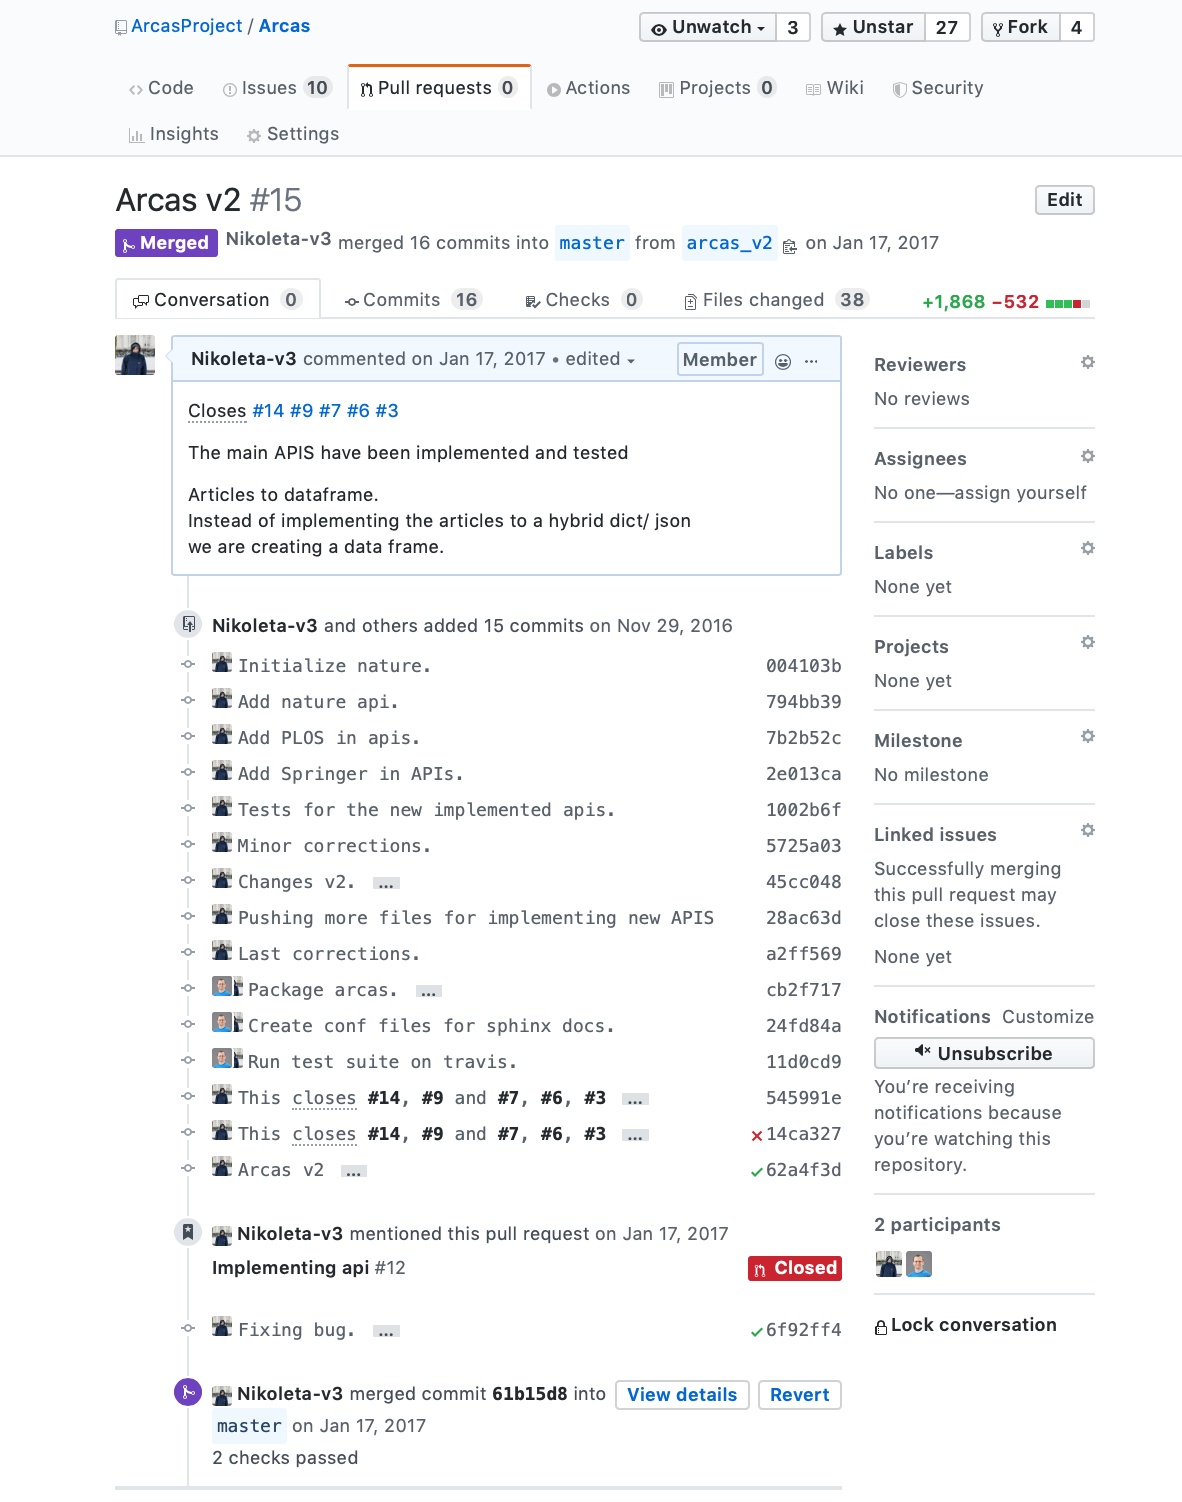
\includegraphics[width=.8\textwidth]{src/chapters/01/img/GitHub_discussion}
    \caption{An example of a pull request on GitHub.}\label{fig:pull_request_github}
\end{figure}

The code for Chapters'~\ref{chapter:bibliometric_study}-\ref{chapter:lstm} is
hosted on individual GitHub repositories,
Table~\ref{table:source_code_data_citations}. The source code for each
repository has been packaged and has been archived on Zenodo~\cite{zenodo}.  % TODO Add a sentence or two here saying what/why archive?

\subsection{Virtual environments}

The source code of each repository has Python libraries as dependencies. Though
several of these projects use the same libraries, the versions of these
libraries can differ. Tracking software dependencies is of paramount importance
in order to ensure the reproducibility of computer code.

There are several tools for keeping dependencies required by different projects
separated. The tool used here are Python \textit{virtual environments}. More
specifically, the Anaconda virtual environments which integrate easily with the
programming language Python. Anaconda~\cite{anaconda} is a free and open-source distribution of
the Python and R programming languages for scientific computing, that aims to
simplify package management and deployment. Package versions are managed by the
package management system conda.

The Anaconda
distribution manager: conda allows users to create, export, list, remove, and update environments that
have different versions of Python and/or packages installed in them. Switching
or moving between environments is called activating the environment. An environment
can be shared and kept under version control as a file. An example of
such as file is given by Figure~\ref{fig:environment_file}.

\begin{figure}
\begin{shell}
name: opt-mo
channels:
  - defaults
dependencies:
  - python=3.6.7
  - numpy=1.15.4
  - pandas=0.23.4
  - pip:
    - attrs==19.1.0
    - axelrod==4.4.0
    - black==18.9b0
    - sympy==1.2.0
    - scikit-optimize==0.5.2
    - jupyter==1.0.0
    - jupyter-console==5.2.0
    - ipython==6.4.0
    - pytest==4.0.1
    - pytest-cov==2.7.1
    - sqlalchemy==1.2.17
    - fsspec==0.3.3
\end{shell}
\caption{An example of an environment file. The name of the specific environment is called
\mintinline{shell}{opt-mo} and it corresponds to the environment associated with
Chapter~\ref{chapter:memory_one}.}\label{fig:environment_file}
\end{figure}

Each chapter of the thesis includes an environment file detailing the dependencies
of the source code and their versions.

\subsection{Automated testing}

Testing code is of considerable importance in order to ensure the robustness,
correctness and sustainability of the computer code. The standard method of testing code is through
\textit{automated testing} using test suits that run parts of the code and
assert whether they are behaving as expected.

Two types of tests are described in~\cite{Percival2014}, \textit{functional
tests} that assert the code's functionality, and \textit{unit tests} that help
ensure the code is clean and free of bugs.

Functional tests aim to test how the whole application functions from the
perspective of the outside user. They feed in basic input and test whether the
end product/final behaviour is as expected. Unit tests assert that small chunks
of code behave as expected, and the test the application from the point of the
programmer. Unit tests are isolated from the rest of the code and are modular.
There are two types of unit tests: \textit{pure} and \textit{integrated} tests.

Pure unit tests are written to test only one function or method. Thus, if a pure
unit test was to fail then it should be due to problems with the specific part
of the code it is testing only, and not any other bit of code. Pure unit tests
are fast and readable, however they do not test how well functions and methods
integrate with one another. In order to test these, unit tests must be written
that rely on other parts of the code that are not explicitly being tested. This
type of test is called integrated tests.

The automated tests, which include functional and unit tests, of the
repositories associated with the thesis have been implemented using the Python
library \mintinline{python}{pytest}. The \mintinline{python}{pytest} framework
makes it easy to write automated tests in a few lines. A plugin to
\mintinline{python}{pytest} is that of \mintinline{python}{pytest-cov}. The plugin
allows for coverage checks. Coverage is a measure used to describe how much of
the code is executed (covered) by the testing suite.

To regularly test code which aims to be merged back into the original codebase
continuous integration (CI) systems are used. CIs perform the tests suite and
the coverage check every time a new version of the codebase is made available
(``pushed'') on GitHub. The benefits of using a CI are identifying bugs quickly,
reducing problems when merging in contributions from collaborators, and adding
transparency to the development process. There are two CIs that have been used
in the repositories listed in Table~\ref{table:source_code_data_citations}.
These are Travis~\cite{travis} and GitHub Actions~\cite{github_actions}.

\subsection{Documentation}

Software \textit{documentation} is written text or illustration that accompanies
computer software or is embedded in the source code. The documentation either
explains how the software operates or how to use it.

Each repository associated with the thesis includes a detailed README file.
These contain installation instructions for corresponding packaged source code
and demonstrate how to run the associated test suite. The source code for each
repository has been written in a modular way and meaningful names have been
given to all variables, functions, methods and classes. Each function, method
and class includes a \text{docstring}. A docstring is a series of sentences used
to document a specific segment of code.

The repositories also include a series of Jupyter Notebooks~\cite{jupyter} that
are used to carry out the analysis of each Chapter, and serve as demonstration
of the source code's usage.

\subsection{Summary of software written}

As previously stated the source code for
Chapters~\ref{chapter:bibliometric_study}-\ref{chapter:lstm} have been written
following best practices, have been packaged, are available on GitHub and have
been archived on Zenodo. These practices have been followed to reassure the the
correctness, reproducibility and sustainability of the source code and research
described throughout the thesis.

To ensure the reproducibility of the work the data sets used in several of
the following Chapters have also been archived and are available online. The details
for the source code and data sets for each Chapter are summarised in
Table~\ref{table:source_code_data_citations}.

\begin{table}[htbp]
    \centering
    \resizebox{\textwidth}{!}{
    \begin{tabular}{clcc}
        \toprule
        {} & GitHub url & Source code citation & Data citation \\
        \midrule
        Chapter~\ref{chapter:bibliometric_study}    & \url{https://github.com/Nikoleta-v3/bibliometric-study-of-the-prisoners-dilemma} &
        \cite{nikoleta_2017} &  \cite{auction_data_2018, anarchy_data_2018, pd_data_2018}\\
        Chapter~\ref{chapter:meta_tournaments}      & \url{https://github.com/Nikoleta-v3/meta-analysis-of-prisoners-dilemma-tournaments} &
        & \cite{data} \\
        Chapter~\ref{chapter:memory_one}            & \url{https://github.com/Nikoleta-v3/Memory-size-in-the-prisoners-dilemma}  & \cite{Glynatsi2019_opt_mo} & \cite{glynatsi2019} \\
        Chapter~\ref{chapter:best_response_sequence}
        \&~\ref{chapter:lstm}                       & \url{https://github.com/Nikoleta-v3/Training-IPD-strategies-with-RNN}   &  & \cite{Glynatsi2020_sequences} \\
        \bottomrule
    \end{tabular}}
    \caption{Citations and GitHub url for source code and data used in the thesis.}
    \label{table:source_code_data_citations}
\end{table}

Throughout the thesis, parts of the source code and examples of it's usage are
going to be presented in the corresponding Chapters. Two types of code snippets
are used in this thesis to present code. Code snippets that demonstrate the
source code of a specific piece of software, Figure~\ref{figure:source_code_example}, and
code snippets that demonstrate the usage,
Figure~\ref{figure:usage_code_example}. These can be distinguish by the three arrows,
\mintinline{python}{>>>}, which are only found in the usage code snippets.
The three arrows are followed by a command. It
demonstrates that the command is executed in a Python interpreter, and the result of executing the command
is the one in the following lines without the arrows.
The code snippets can also be distinguish by their background color. The usage
snippets have a darker background.

\begin{figure}[htbp]
\begin{sourcepy}
import axelrod as axl

def simulate_match_utility(player, opponent, turns=500, repetitions=200):
    """
    Returns the simulated utility of a memory one player against a single opponent.
    """
    total = 0
    players = [axl.MemoryOnePlayer(vector) for vector in [player, opponent]]
    for rep in range(repetitions):
        match = axl.Match(players=players, turns=turns)
        _ = match.play()

        total += match.final_score_per_turn()[0]

    return total / repetitions
\end{sourcepy}
\caption{Example of a function implemented withing the package
\mintinline{python}{opt_mo} which is the package that has been developed to
carry out the research of Chapter~\ref{chapter:memory_one}.}\label{figure:source_code_example}
\end{figure}

\begin{figure}[htbp]
\begin{usagepy}
>>> import opt_mo
>>> opt_mo.utility.simulate_match_utility([1, 0, 1, 0], [1, 1, 1, 1])
3.0

\end{usagepy}
\caption{An example of using the function \mintinline{python}{simulate_match_utility}
given by Figure~\ref{figure:source_code_example}.}\label{figure:usage_code_example}
\end{figure}

The results of this thesis heavily rely not only on the projects of
Table~\ref{table:source_code_data_citations} but also on the open source package
Axelrod-Python library (APL). APL~\cite{axelrodproject} is an open source
project for simulating rounds of the IPD which contains a large collections of
strategies. APL has several capabilities which include performing different
types of tournaments. Its documentation is found at
\url{http://axelrod.readthedocs.io/}. The specific version of APL used at each
Chapter will be mentioned at the start of each Chapter.

This thesis itself is hosted on a GitHub repository at
\url{https://github.com/Nikoleta-v3/Thesis}. It is written in the document
preparation system \LaTeX, and automated tests have been setup to test
that the document compiles, spelling is correct, every time
an updated version of the document is pushed to GitHub. The usage code examples
of this thesis are also automatically tested. Each command beginning with the
symbol \mintinline{python}{>>>} is executed each time the document is pushed to GitHub.
The test executes the commands and checks that the outcome is the
same as the one following the command in the code snippets.

\section{Chapter Summary}

This Chapter has introduced the Iterated Prisoner's Dilemma which is the
strategic game used in this thesis. It has presented a review of the Axelrod's
tournaments in the 1980s, and presented a list of tournaments that have been
performed ever since.

The research questions of this thesis and how each Chapter contributes to these
questions have been outlined. The research of this thesis heavily reliefs on
software. The software include already established packages and packages that
have been developed specifically for this thesis. These have been developed
following best practices. A number of best practices were introduced in
section~\ref{section:introduction_software_development}.

The software packages and the data sets used in the following Chapters have been
archived and made available online. This reassures that all the results
presented in the following Chapters are reproducible. The developed packages as
well as this thesis are being hosted on GitHub repositories and are being tested
using automated tests.

\chapter{A systematic literature review of the Prisoner's Dilemma.}\label{chapter:literature_review}

\section{Introduction}

Chapter~\ref{chapter:introduction} introduced the Prisoner's Dilemma as the main
game theoretic model that will be used throughout this thesis, and presented a
brief literature review of the research this thesis is building upon. This
Chapter provides a more detailed systematic literature on the Prisoner's
Dilemma. The aim of this Chapter is to provide a concrete summary of the
existing literature and to identify research topics in the field of the PD. This is
achieved by partitioning the literature in five different sections each
reviewing a different aspect of research. The Chapter is structured as follows:

\begin{itemize}
    \item section~\ref{section:origin} presents the origin of the PD
    and reviews the early publications in the field and the use of
    human subject research.
    \item section~\ref{section:intelligent_design} presents the pioneering computer
    tournaments of Robert Axelrod and reviews IPD strategies of intelligent design.
    \item section~\ref{section:evolutionary_dynamics} discusses
    the emergence, or not, of cooperative behaviour in evolutionary dynamics.
    \item section~\ref{section:structured_strategies} defines structured
    strategies in the IPD, the notion of training and discusses related papers.
    \item section~\ref{section:software} reports on educational and research software
    used for simulating the PD game.
\end{itemize}

\section{Origins of the prisoner's dilemma}\label{section:origin}

The origin of the PD goes back to the 1950s in early experiments conducted at
RAND~\cite{Flood1958} to test the applicability of games described
in~\cite{VonNeumann1944}. The game received its name later the same year.
According to~\cite{Tucker1983}, Albert W. Tucker (the PhD supervisor of John
Nash~\cite{Nash1951}), in an attempt to deliver the game with a story during a
talk described the players as prisoners and the game has been known as the
Prisoner's Dilemma ever since.

The early research on the IPD was limited. The only source of
experimental results was through human subject research where pairs of
participants simulated plays of the game, and human subject research had
disadvantages. Humans could behave randomly and in several experiments both the
size and the background of the individuals were different, thus comparing
results of two or more studies became difficult.

The main aim of these early research experiments was to understand how
conditions such as the gender of the participants~\cite{Evans1966, Lutzker1961,
Mack1971}, the physical distance between the participants~\cite{Sensenig1972}, the
effect of their opening moves~\cite{Tedeschi1968} and even how the experimenter, by varying
the tone of their voice and facial expressions~\cite{Gallo1968}, could influence
the outcomes and subsequently the emergence of cooperation. An early figure that
sought out to understand several of these conditions was the mathematical
psychologist Anatol Rapoport. The results of his work are summarised
in \cite{rapoport1965}.

Rapoport was also interested in conceptualising strategies that could promote
international cooperation. Decades later he would submit the winning strategy
(Tit for Tat) of the first computer tournament, run by Robert Axelrod.
These tournaments and several strategies that were designed by researchers, such
as Rapoport, are introduced in the following section.

\section{Axelrod's tournaments and intelligently designed strategies}
\label{section:intelligent_design}

As discussed in Section~\ref{section:origin}, before 1980 a great deal of
research was done in the field, however, as described in~\cite{Axelrod2012}, the
political scientist Robert Axelrod believed that there was no clear answer to the
question of how to avoid conflict, or even how an individual should play the
game. Combining his interest in artificial intelligence and political science
Axelrod created a framework for exploring these questions using computer
tournaments and made the study of cooperation of critical interest. As
described in~\cite{Rapoport2015}, ``Axelrod's new approach has been extremely
successful and immensely influential in casting light on the conflict between an
individual and the collective rationality reflected in the choices of a
population whose members are unknown and its size unspecified, thereby opening a
new avenue of research''.

% In a collaboration with a colleague, Douglas Dion,
% Axelrod in~\cite{Axelrod1988} summarized a number of works that were immediately
% inspired from the ``Evolution of Cooperation''

The first reported computer tournament took place in 1980~\cite{Axelrod1980a}. 
Axelrod asked researchers to design a strategy with the purpose of winning an IPD
tournament. A
total of 13 strategies were submitted, written in the programming languages
Fortran or Basic. Each competed in a 200 turn match against all 12 opponents,
itself and a player that played randomly (called \textit{Random}). This type of
tournament is referred to as a \textit{round robin}. The tournament was repeated 5 times
to get a more stable estimate of the scores for each pair of play.
Each participant knew the exact number of turns and had access to the full
history of each match. Furthermore, Axelrod performed a preliminary tournament
and the results were known to the participants. This preliminary tournament is
mentioned in~\cite{Axelrod1980a} but no details were given.

The winner of the tournament was determined by the total average score and not
by the number of matches won. The strategy that was announced the winner was the
strategy submitted by Rapoport, \textit{Tit For Tat}. The success of Tit for Tat
came as a surprise. It was not only the simplest submitted strategy, it would
always cooperates on the first round and then mimic the opponent's previous
move, but it had also won the tournament even though it could never beat
any player it was interacting with.

In order to further test the results Axelrod performed a second tournament
in 1980~\cite{Axelrod1980b}. The second tournament received much more attention
and had a total of 62 entries. The participants knew the results of the previous
tournament and the rules were similar with only a few alterations. The
tournament was repeated 5 times and the length of each match was not known to
the participants. Axelrod intended to use a fixed probability (refereed to as
`shadow of the future'~\cite{Axelrod1988}) of the game ending on the next move.
However, 5 different number of turns were selected for each match 63, 77, 151,
308 and 401, such that the average length would be around 200 turns.

Nine of the original participants competed again in the second tournament. Two
strategies that remained the same were Tit For Tat and \textit{Grudger}. Grudger
is a strategy that will cooperate as long as the opponent does not defect,
submitted by James W. Friedman. The name Grudger was give to the strategy
in~\cite{Li20141}, though the strategy goes by many names in the literature such
as, Spite~\cite{Beaufils1997}, Grim Trigger~\cite{Banks1990} and
Grim~\cite{Van2015}. New entries in the second tournament included \textit{Tit
for Two Tats} submitted by John Maynard Smith and \textit{KPavlovC}. KPavlovC,
is also known as Simpleton~\cite{rapoport1965}, introduced by Rapoport or just
Pavlov~\cite{Nowak1993}. The strategy is based on the fundamental behavioural
mechanism win-stay, lose-shift. Pavlov is heavily studied in the literature and
similarly to Tit for Tat it is used in tournaments today and has
had many variants trying to build upon it's success, for example
\textit{PavlovD} and \textit{Adaptive Pavlov}~\cite{Li2007}.

Despite the larger size of the second tournament none of the new entries managed
to outperform the simpler designed strategy. The winner was once again Tit for
Tat. Axelrod deduced the following guidelines for a strategy to perform well:

\begin{itemize}
    \item The strategy would start of by cooperating.
    \item It would forgive it's opponent after a defection.
    \item It would always be provoked by a defection no matter the history.
    \item It was simple.
\end{itemize}

The success of Tit for Tat, however, was not unquestionable. Several papers
showed that stochastic uncertainties severely undercut the effectiveness of
reciprocating strategies and such stochastic uncertainties have to be expected
in real life situations~\cite{Milinski1987}. For example, in~\cite{Molander1985}
it is
proven that in an environment where \textit{noise} (a probability that a
player's move will be flipped) is introduced two strategies playing Tit for Tat
receive the same average payoff as two Random players.
Hammerstein, pointed out that if by mistake, one of two
Tit for Tat players makes a wrong move, this locks the two opponents into a
hopeless sequence of alternating defections and cooperations~\cite{Hammerstein1984}.
The poor performance of the strategy in noisy environments was also demonstrated
in tournaments. In~\cite{Bendor1991, Donninger1986} round robin
tournaments with noise were performed, and Tit For Tat did not win.
The authors concluded that to overcome the noise more generous strategies
than Tit For Tat were needed. They introduced the strategies \textit{Nice and Forgiving}
and \textit{OmegaTFT} respectively.
A second type of stochastic uncertainty is
misperception, where a player's action is made correctly but it is recorded
incorrectly by the opponent. In~\cite{Wu1995}, a strategy
called~\textit{Contrite Tit for Tat} was introduced that was more successful than Tit for Tat
in such environments. The difference between the strategies was that Contrite
Tit for Tat was not so fast to retaliate against a defection.

Several works extended the reciprocity based approach which has led to new
strategies. For example Gradual~\cite{Beaufils1997} which was constructed to
have the same qualities as those of Tit for Tat except one,
\textit{Gradual} had a memory of the game since the beginning of it. Gradual
recorded the number of defections by the opponent and punished them with a
growing number of defections. It would then enter a calming state in which it
would cooperates for two rounds. In a tournament of 12 strategies, including
both Tit for Tat and Pavlov, Gradual managed to outperformed them all. A
strategy with the same intuition as Gradual is \textit{Adaptive Tit for
Tat}~\cite{tzafestas-2000a}. Adaptive Tit for Tat does not keep a permanent
count of past defections, it maintains a continually updated estimate of the
opponent’s behaviour, and uses this estimate to condition its future actions. In
the exact same tournament as in~\cite{Beaufils1997} with now 13 strategies Adaptive
Tit for Tat ranked first.

Another extension of strategies was that of teams of
strategies~\cite{J.P.Delahaye1993Lp, J.P.Delahaye1995LIeP, A.Rogers2007Ctpw}
that collude to increase one member's score. In 2004 Graham Kendall led the
Anniversary Iterated Prisoner's Dilemma Tournament with a total of 223 entries.
In this tournament participants were allowed to submit multiple strategies. A
team from the University of Southampton submitted a total of 60
strategies~\cite{A.Rogers2007Ctpw}. All these were strategies that had been
programmed with a recognition mechanism by default. Once the strategies
recognised one another, one would act as leader and the other as a follower. The
follower plays as a \textit{Cooperator}, cooperates unconditionally and the
leader would play as a \textit{Defector} gaining the highest achievable score.
The followers would defect unconditionally against other strategies to lower
their score and help the leader. The result was that Southampton had the top
three performers. Nick Jennings, who was part of the team, said that ``We
developed ways of looking at the Prisoner's Dilemma in a more realistic
environment and we devised a way for computer agents to recognise and collude
with one another despite the noise. Our solution beats the standard Tit For Tat
strategy"~\cite{southampton_blog}.

\subsection{Memory-one Strategies}\label{section:memory_one}

A set of strategies that have received a lot of attention in
the literature are \textit{memory-one} strategies. In~\cite{Nowak1989},
Nowak and Sigmund proposed a structure for studying simple strategies that
remembered only the previous turn, and moreover, only recorded the move of the
opponent. These are called \textit{reactive} strategies and they can be
represented by using three parameters \((y, p_1, p_2)\), where \(y\) is the
probability to cooperate in the first move, and \(p_1\) and \(p_2\) are the
conditional probabilities to cooperate given that the opponent's last move was
a cooperation or a defection. For example Tit For Tat is a reactive strategy and
it can be written as \((1, 1, 0)\). Another reactive strategy well known in
the literature is \textit{Generous Tit for Tat}~\cite{Nowak1992} (\(1, 1, \frac{1}{3}\)).

In~\cite{Nowak1990}, Nowak and Sigmund extended
their work to include strategies which consider the entire history of the previous turn to make a decision.
These are called memory-one strategies.
If only a single turn of the game is taken into account and depending on the
simultaneous moves of the two players there are only four possible states that
the players could be in. These are:

\begin{itemize}
    \item Both players cooperated, denoted as \(CC\).
    \item First player cooperated while the second one defected, denoted as \(CD\).
    \item First player defected while the second one cooperated, denoted as \(DC\).
    \item Both players defected, denoted as \(DD\).
\end{itemize}

Thus, a memory-one strategy can be denoted by the probabilities of cooperating
after each state and the probability of cooperating in the first round, \((y,
p_1, p_2, p_3, p_4)\). For example Pavlov's memory-one representation is \((1,
1, 0, 0, 1)\). Though reactive and memory-one strategies have to specify their
move in the first round, the opening move is a transient effect and has no affect
on the game in long run~\cite{sigmund2010calculus}. Consequently, reactive strategies
can be described as elements \(p \in R^2\) and memory-one strategies as \(p \in R^4\).

Memory-one strategies made an impact when a specific subset of memory-one
strategies were introduced called \textit{Zero-determinant} strategies
(ZDs)~\cite{Press2012}. The American Mathematical Society's news section~\cite{Hilbe2015}
stated that ``the world of game theory is currently on fire'' and in~\cite{Stewart2012}
it was stated that
``Press and Dyson have fundamentally changed the viewpoint on the Prisoner's Dilemma''.
ZDs are a set of
extortionate strategies that can force a linear relationship between
the long-run scores of both themselves and the opponent, therefore ensuring that the
opponent will never do better than them. Press and Dyson's suggested that the ZDs
were the dominant set of strategies in the
IPD, and as memory did not benefit them then they argued that memory is not beneficial for any strategy. In~\cite{Adami2013, Knight2017,
Hilbe2013, Hilbe2013b, Hilbe2015, KnightHGC17, Knight2019, Lee2015, Stewart2012} the
effectiveness of ZDs is questioned. Namely,~\cite{Stewart2013, Stewart2016}
showed that memory-one strategies must be forgiving to be evolutionarily stable
and~\cite{Knight2017, Hilbe2017, KnightHGC17, Knight2019, Lee2015, Pan2015} demonstrated
that longer-memory strategies have an advantage over short memory
strategies. Chapter~\ref{chapter:memory_one}, studies the set of memory-one strategies,
and more specifically, best response memory-one strategies and reinforces the
discussion that the best action is adaptability and not manipulation, and short
memory can be limiting.

This section of the literature covered the original computer tournaments of
Axelrod, the early success of Tit For Tat in these tournaments and excessive
amounts of IPD strategies. Though Tit For Tat was
considered to be the most robust basic strategy, reciprocity was found to not
be enough in environments with uncertainties. There are at least two properties,
that have been discussed in this section, for coping with such uncertainties;
generosity and contrition. Generosity is letting a percentage of defections go
unpunished, and contrition is lowering a strategy's readiness to defect
following an opponent's defection. The strategies covered in this section are all
strategies of intelligent design. They have been designed by researchers and
not surfaced from an indirect process, such strategies are covered in
section~\ref{section:structured_strategies}.

In the later part of this section a series of new strategies which were built on
the basic reciprocal approaches were presented, followed by the infamous memory-one
strategies, the zero-determinant strategies. Though the ZDs can be proven to be robust
in pairwise interactions they were found to be lacking in evolutionary settings
and in computer tournaments. Evolutionary settings and the emergence
of cooperation under natural selection are covered in the next section.

\section{Evolutionary dynamics}\label{section:evolutionary_dynamics}

As yet, the emergence of cooperation has been discussed in the contexts of the
one shot PD game (Chapter~\ref{chapter:introduction}) and the IPD round robin
tournaments (Sections~\ref{section:intelligent_design}). In the PD it is
known that cooperation will not emerge, furthermore, in a series of influential works
Axelrod demonstrated that reciprocal behaviour favours cooperation when
individuals interact repeatedly. But does natural selection favour cooperation?
Understanding the conditions under which natural selection can favour
cooperative behaviour is important in understanding social behaviour amongst
intelligent agents~\cite{Boyd1987}.

Imagine a mixed population of cooperators and defectors where every
time two individuals meet they play a game of PD. In such population the average
payoff for defectors is always higher than cooperators. Under natural selection
the frequency of defectors will steadily increase until cooperators become
extinct. Thus natural selection favours defection in the PD
(Figure~\ref{fig:natural_selection_diagram}), however, there are several mechanisms
that allow the emergence of cooperation in an evolutionary context which will be
covered in this section.

\begin{figure}[!hbtp]
    \centering
    \includestandalone{src/chapters/02/tex/natural_selection}
    \caption{Natural selection favours defection in a mixed population of Cooperators
    and Defectors.}\label{fig:natural_selection_diagram}
\end{figure}

In the later sections of~\cite{Axelrod1980b}, Axelrod discusses an
ecological tournament that he performed using the 62 strategies of the second
tournament to understand the reproductive success of Tit for Tat. In an
ecological tournament the prevalence of each type of strategy in each round was
determined by that strategy's success in the previous round. The competition in
each round would become stronger as weaker performers were reduced and
eliminated. The ecological simulation concluded with a handful of nice
strategies dominating the population whilst exploitative strategies had died off.
That was because the weaker strategies which were being exploitative were becoming
extinct, and exploitative strategies were loosing their prey.

This new result led Axelrod to
study the IPD in an evolutionary context based on several of the approaches
established by the biologist John M. Smith~\cite{Smith1974,
Smith1979, Smith1973}. John M. Smith was a fundamental figure in evolutionary game theory and a
participant of Axelrod's second tournament. The biological applications of the
new evolutionary approach~\cite{Axelrod1981} won Axelrod and his co-author William
Donald Hamilton the
Newcomb-Cleveland prize of the American Association for the Advancement of
Science.
In~\cite{Axelrod1981} pairs of individuals from a
population played the IPD. The number of interactions between the pairs were
not fixed, but there was a probability defined \(w\), where \(0 < w < 1\), that the pair would interact again. This was referred to as the \textit{importance of the future}
of the game. It
was shown that for
a sufficient high \(w\) Tit For Tat strategies
would become common and remain common because they were ``collectively stable".
Axelrod argued that collective stability implied evolutionary stability (ESS)
and that when a collectively stable strategy is common in a population and
individuals are paired randomly, no other rare strategy can invade. However,
Boyd and Lorderbaum in~\cite{Boyd1987} proved that if \(w\), the importance of the
future of the game, is large enough then no pure strategy is ESS because it can
always be invaded by any pair of other strategies. This was also independently
proven in~\cite{Pudaite1987}.

All these conclusions were made in populations where the individuals could all
interact with each other. In 1992, Nowak and May, considered a structured population
where an individual's interactions were limited to its neighbours.
More specifically, in~\cite{Nowak1992b} they explored how local interaction
alone can facilitate population wide cooperation in a one shot PD game. The two
deterministic strategies Defector and Cooperator, were placed onto a two
dimensional square array where the individuals could interact only with the
immediate neighbours. The number of immediate neighbours could be either,
fourth, six or eight, as shown in Figure~\ref{fig:topologies}, where each node
represents a player and the edges denote whether two players will interact. This
topology is refereed to as \textit{spatial topology}. Each cell of the lattice is
occupied by a Cooperator or a Defector and at each generation step each cell owner
interacts with its immediate neighbours. The score of each player is calculated
as the sum of all the scores the player achieved at each generation. At the
start of the next generation, each lattice cell is occupied by the player with
the highest score among the previous owner and their immediate neighbours.

\begin{figure}[!hbtp]
    \centering
        \begin{subfigure}{.25\textwidth}
            \includestandalone[width=\textwidth]{src/chapters/02/tex/square_lattice}
        \end{subfigure}
        \begin{subfigure}{.25\textwidth}\centering
            \includestandalone[width=\textwidth]{src/chapters/02/tex/hexagonal_lattice}
         \end{subfigure}
         \begin{subfigure}{.25\textwidth}\centering
            \includestandalone[width=\textwidth]{src/chapters/02/tex/square_lattice_eight}
         \end{subfigure}
         \caption{Spatial neighbourhoods}\label{fig:topologies}
\end{figure}

Limited/Local interactions proved that as long as small clusters of cooperators form, where
they can benefit from interactions with other cooperators while avoiding
interactions with defectors, global cooperation will continue. Thus, local
interactions proved that even for the PD cooperation can emerge. Moreover in
\cite{Ohtsuki2006}, whilst using the donation game (
Equation~(\ref{eq:donation_game})), it was shown that cooperation will
evolve in a structured population as long as the benefit to cost ratio \(b / c\)
is higher than the number of neighbours.

In structured populations local interactions that can dynamically change were
considered in~\cite{Perc2011}. Graphs with a probability of rewiring 
connections were considered, and the rewire could be with any given node in the
graphs and not just with immediate neighbours. Perc et al. concluded that
``making new friends'' may be an important activity for the successful evolution
of cooperation, but also they must be selected carefully and one should keep
their number limited.

Another approach for increasing the likelihood of cooperation by increasing of
assortative interactions among cooperative agents, include partner identification
methods such as reputation~\cite{Janssen2006, Nowak1998, Suzuki2005},
communication tokens~\cite{Miller2002} and tags~\cite{Choi2006, Hales2000,
Miller2002, Riolo2001}.

This section considered papers on evolutionary dynamics and mechanisms that ensure
the emergence, or not, of cooperation. The following section focuses on strategy
archetypes, training methods and strategies obtained from training.

\section{Structured strategies and training}
\label{section:structured_strategies}

This section covers strategies that are different to that of intelligent design discussed
in Section~\ref{section:intelligent_design}. These are strategies that have
been through a \textit{training process} using generic strategy archetypes. For example,
in~\cite{Axelrod1987} Axelrod explored deterministic strategies that
took into account the last 3 plays of both players. As discussed in
Section~\ref{section:memory_one}, for each turn there are 4 possible outcomes,
\(CC, CD, DC, DD\), thus for 3 turns there are a total of
\(4\times4\times4=64\) possible combinations. Therefore, the strategy can be
defined by a series of 64 C's/D's, corresponding to each combination; this type
of strategy is called a \textit{lookup table}. A graphical representation of the
look up table strategy in~\cite{Axelrod1987} is given by Figure~\ref{fig:lookup_table_diagram}.
In~\cite{Axelrod1987} lookup tables were trained using a
genetic algorithm~\cite{Koza1997}. A training process includes making random changes to
a given instant of the lookup table, Figure~\ref{fig:lookup_table_diagram_choice}.
The strategy which corresponds to the new altered
instant is evaluated in a given setting set by the experiment, and if the
utility of the strategy has increased this change is kept and its genes are passed 
on to a new generation of strategies.
A genetic algorithm is not the only heuristic method which can be used for
training strategies, realistically any heuristic method can be used.


\begin{figure}[!hbtp]
    \begin{subfigure}{.45\textwidth}\centering
        \includestandalone[width=.30\textheight]{src/chapters/02/tex/lookup_table_diagram}
        \caption{A graphical representation of a look up table player which considers
        3 plays of both players.}\label{fig:lookup_table_diagram}
    \end{subfigure}\hspace{.5cm}
    \begin{subfigure}{.45\textwidth}\centering
        \includestandalone[width=.30\textheight]{src/chapters/02/tex/lookup_table_diagram_choice}
        \caption{Training a look up table player includes making changes to the
        strategy's responses to a history.}\label{fig:lookup_table_diagram_choice}
     \end{subfigure}
     \caption{A graphical representation of the lookup table strategy described
     in~\cite{Axelrod1987}, and a demonstration of the changes a strategy exhibits
     during training.}\label{fig:lookup_table}
\end{figure}

In 1996 John Miller considered finite state automata as an
archetype~\cite{Miller1996}, more specifically, Moore
machines~\cite{moore1956}. The training process used a genetic algorithm and
the strategies were evaluated in a tournament with noise.
Miller's results showed that even a small
difference in noise (from 1\% to 3\%) significantly changed the characteristics
of the evolving strategies. The strategies he introduced were \textit{Punish
Twice}, \textit{Punish Once for Two Tats} and \textit{Punish Twice and Wait}.
A training combination of finite state automata and a genetic algorithm was
also considered in~\cite{Ashlock2006b}. In a series of experiments where the size of
the population varied, there were two strategies frequently developed by the
training process and more over they were developed only after the evolution had
gone on for many generations. These were \textit{Fortess3} and
\textit{Fortess4}.

Also, in 1996 the first structured strategies based on
neural networks that had been trained using a genetic algorithm were introduced
in~\cite{Harrald1996} by Harrald and Fogel. Harrald and Fogel considered a
single layered neural network which had 6 inputs. These were the last 3 moves of
the player and the opponent, similar to~\cite{Axelrod1987}. Neural networks have
broadly been used since 1996 to train IPD strategies~\cite{Ashlock2006a, Chong2005,
Marks1999, Franken2005} with training methods such as genetic
algorithms~\cite{Ashlock2006a, Chong2005, Marks1999, Franken2005} and particle swarm
optimization~\cite{Franken2005}. Chapter~\ref{chapter:lstm} of this thesis discusses
the training of strategies using neural network in more details, as the aim of
the chapter is to use an extension of a neural network, a
\textit{recurrent neural network}, to train an IPD strategy.

In~\cite{Knight2017, KnightHGC17} both genetic algorithm and particle swarm
optimization were used to introduce a series of structured strategies based on
lookup tables, finite state machines, neural networks, hidden Markov
models~\cite{eddy1996} and Gambler. Hidden Markov models, are a stochastic
variant of a finite state machine and Gamblers are stochastic variants of lookup
tables. The structured strategies that arised from the training were put up
against a large number of strategies in (1) a Moran process, which is an
evolutionary model of invasion and resistance across time during which high
performing individuals are more likely to be replicated and (2)
a round robin tournament. In a round robin tournament which was simulated using the
software~\cite{axelrodproject} and the 200 strategies implemented within the
software, the top spots were dominated by the trained strategies of all the
archetypes. The top three strategies were \textit{Evolved
LookUp 2 2 2}, \textit{Evolved HMM 5} and \textit{Evolved FSM 16}.
In~\cite{KnightHGC17} it was demonstrated that these trained strategies
would overtake the population in a Moran process. The strategies evolved an ability
to recognise themselves by using a handshake. This recognition mechanism allowed the strategies
to resist invasion by increasing the interactions between themselves, an approach
similar to the one described in Section~\ref{section:evolutionary_dynamics}.

Throughout the different methods of training that have been discussed in this
section, a spectrum of structured strategies can be found. Differentiating
between strategies is not always straightforward. It is not obvious looking at a
finite state diagram how a machine will behave, and many different machines, or
neural networks can represent the same strategy. For example
Figure~\ref{fig:machine_tft} shows two finite automata and both are a
representation of Tit for Tat.

\begin{figure}[!hbtp]
    \begin{subfigure}{.45\textwidth}\centering
        \includestandalone[height=.1\textheight]{src/chapters/02/tex/tit_for_tat_fsm_one}
        \caption{Tit for Tat as a finite state machine with 1 state.}\label{fig:representation_a}
    \end{subfigure}
    \begin{subfigure}{.45\textwidth}\centering
        \includestandalone[height=.1\textheight]{src/chapters/02/tex/tit_for_tat_fsm}
        \caption{Tit for Tat as a finite state machine with 2 states.}\label{fig:representation_b}
     \end{subfigure}
     \caption{Finite state machine representations of Tit for Tat. A machine
     consists of transition arrows associated with the states. Each arrow is
     labelled with \(A/R\) where \(A\) is the opponent's last action and \(R\)
     is the player's response. Finite state machines consist of a set of
     internal states. In (a) Tit for Tat finite state
     machine consists of 1 state and in (b) of 2.}\label{fig:machine_tft}
\end{figure}

To allow for identification of similar strategies a method called
\textit{fingerprinting} was introduced in~\cite{Ashlock2005} by Daniel Ashlock. The method of fingerprinting is a
technique for generating a functional signature for a
strategy~\cite{Ashlock2008}. This is achieved by computing the score of a
strategy against a spectrum of opponents. The basic method is to play the
strategy against a probe strategy with varying noise parameters.
In~\cite{Ashlock2005} Tit for Tat is used as the probe strategy. In
Figure~\ref{fig:fingerprinting} an example of Pavlov's fingerprint is given.
Fingerprinting has been studied in depth in~\cite{Ashlock2008, Ashlock2009,
Ashlock2010, Ashlock2006a}. Another type of fingerprinting is the
\textit{transitive fingerprint}~\cite{axelrodproject}.
The method represents the cooperation rate of a strategy against a set of opponents
over a number of turns. An example of a transitive fingerprint is given in
Figure~\ref{fig:transitive_fingerprinting}.

\begin{figure}[!hbtp]
    \centering
    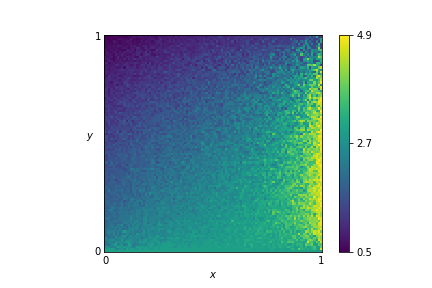
\includegraphics[height=.3\textheight]{src/chapters/02/img/Win-Stay_Lose-Shift}
    \caption{Pavlov fingerprinting with Tit for Tat used as the probe strategy.
    Figure was generated using~\cite{axelrodproject}.}
    \label{fig:fingerprinting}
\end{figure}

\begin{figure}[!hbtp]
    \centering
    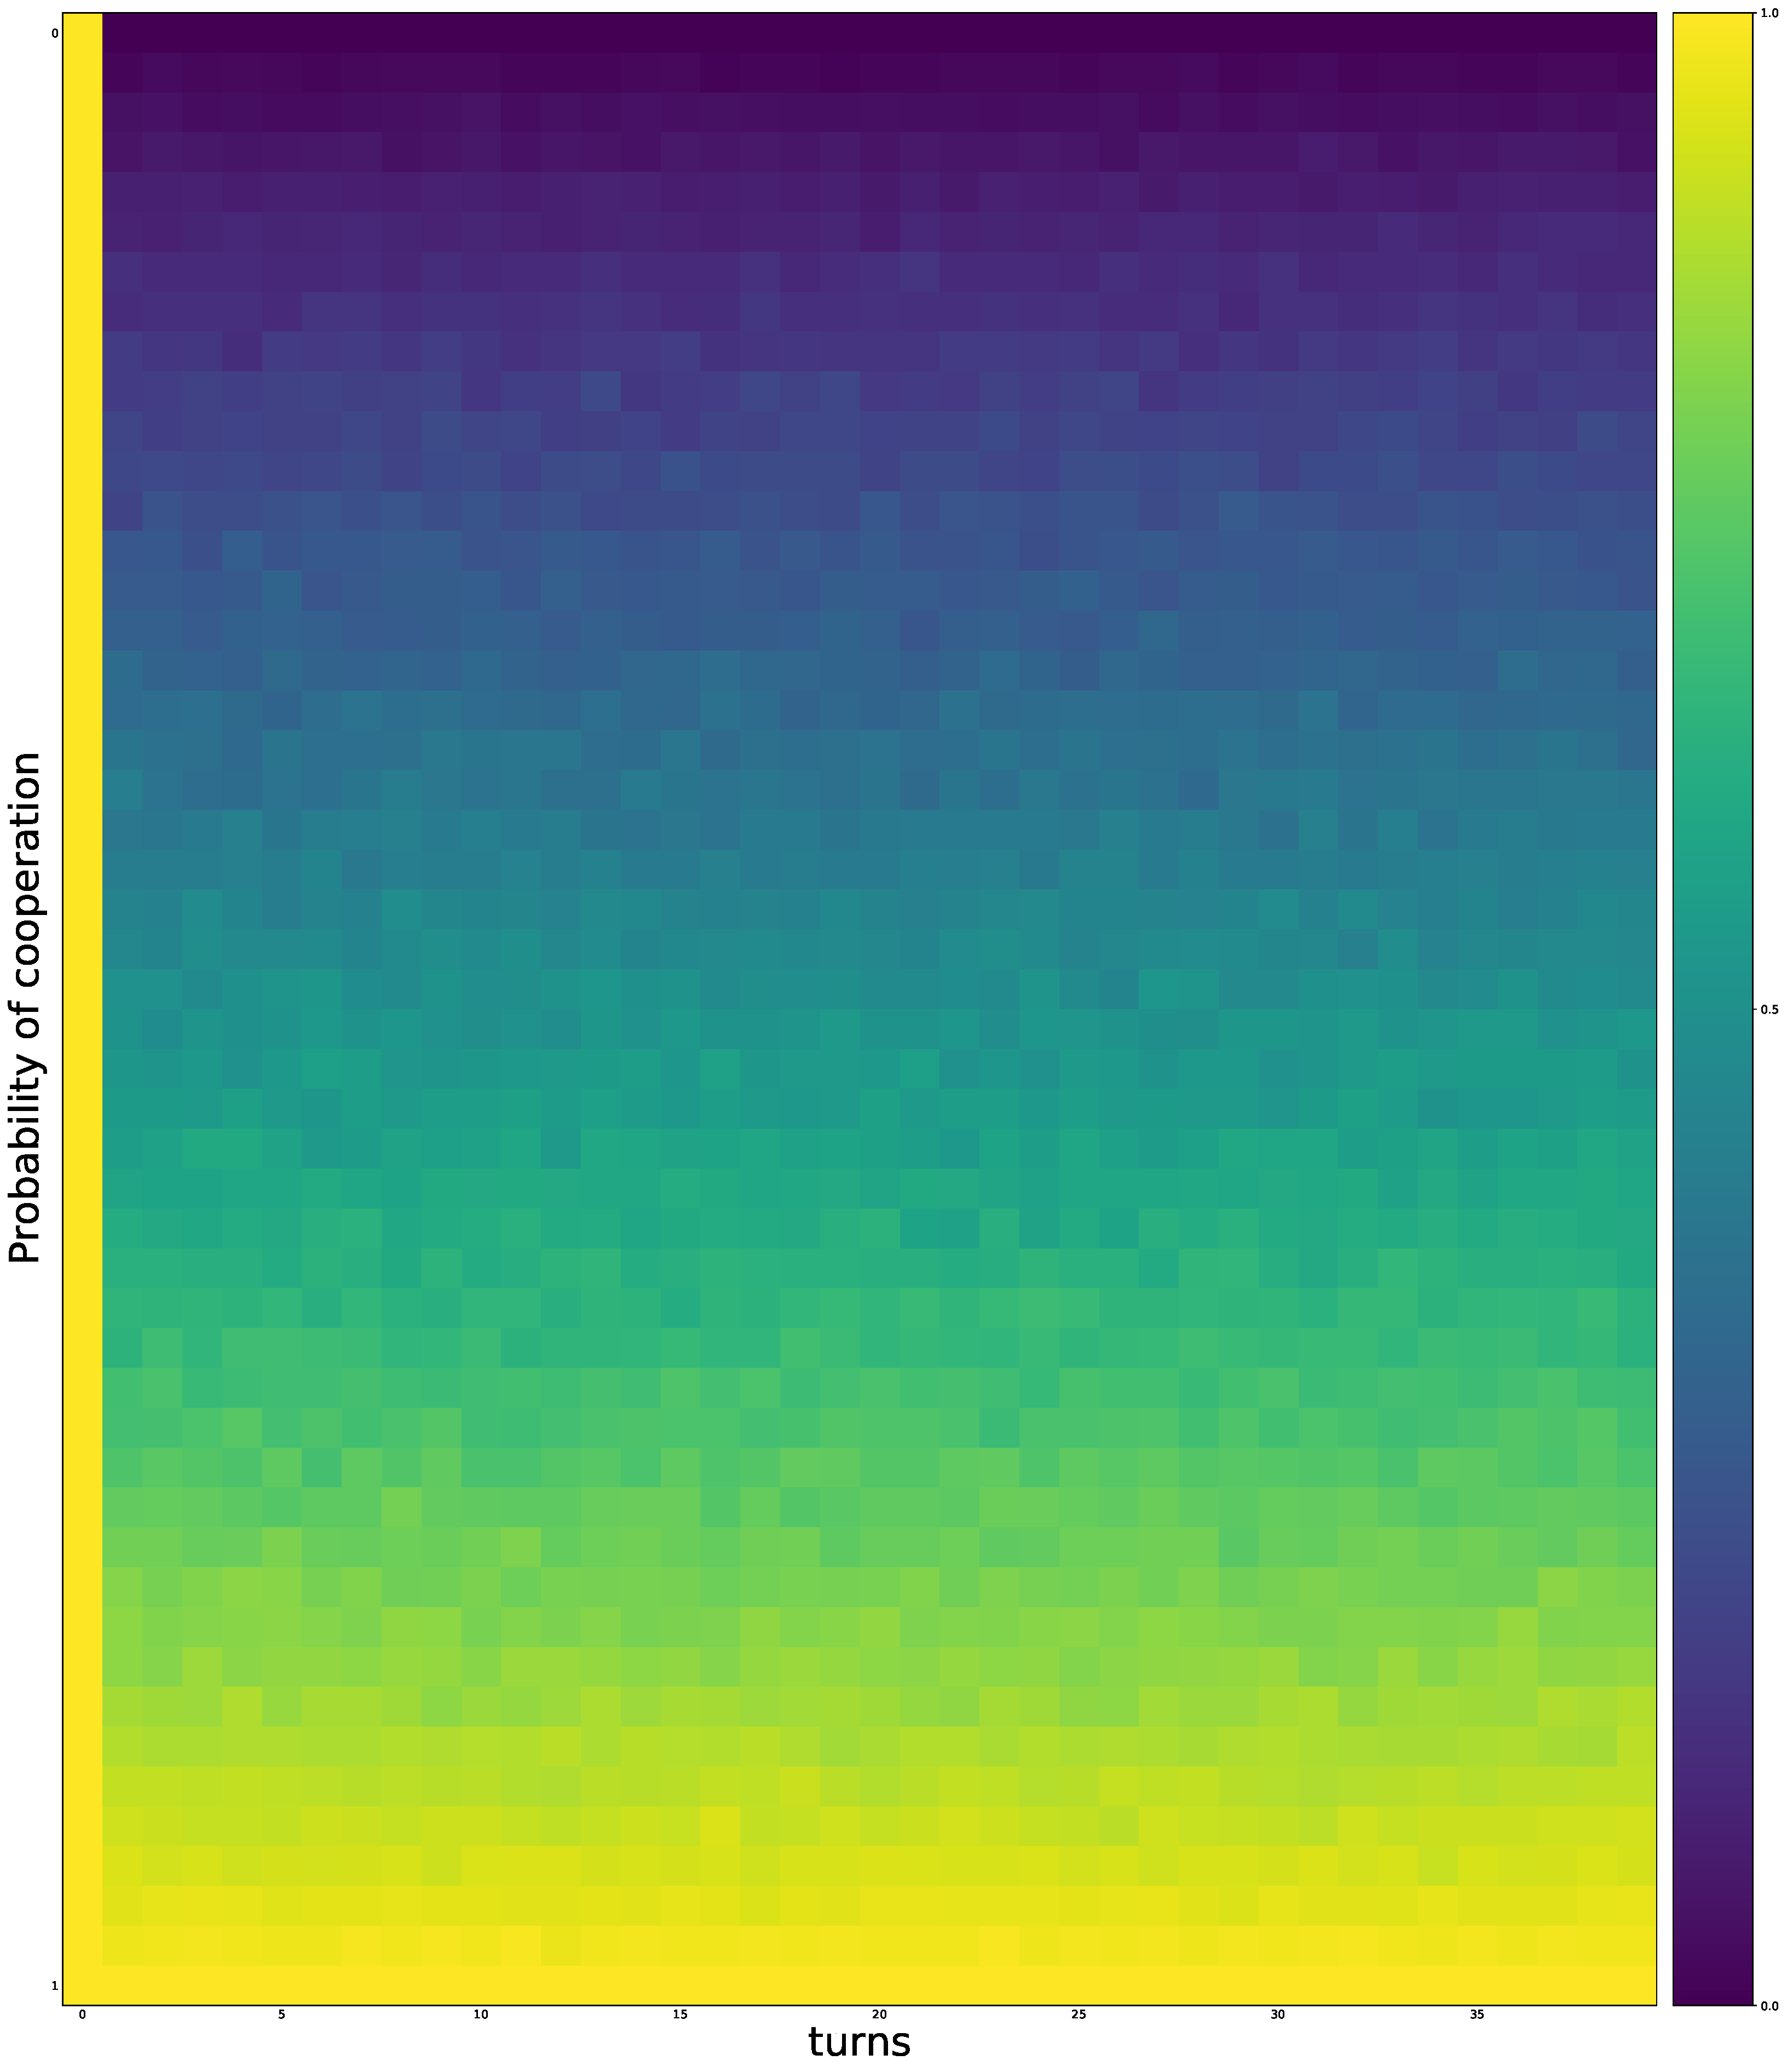
\includegraphics[height=.3\textheight]{src/chapters/02/img/Tit_for_Tat_fingerprint}
    \caption{Transitive fingerprint of Tit for Tat against a set of 50 random opponents
    with varying cooperation rate.}
    \label{fig:transitive_fingerprinting}
\end{figure}

This section covered a series of structured strategies based on different
archetypes which have been trained via different training methods. The works
discussed in this section has demonstrated that through these indirect
training processes successful IPD strategies can emerge. This thesis explores
both strategies of intelligent design (Chapter~\ref{chapter:memory_one}) and
trained strategies (Chapter~\ref{chapter:lstm})in more details. The next section
covers software that has been developed with the main aim of simulating the IPD
interactions.

\section{Software}\label{section:software}

Aside from human subject research the research of the IPD heavily relies on software.
This is to be expected as computer tournaments have become the main
means of simulating the interactions in an IPD game.
Many academic fields suffer from lack of source code availability and the IPD
is not an exception. Several of the tournaments that have been discussed so far were generated
using computer code, though not all of the source code is available.
The code for Axelrod's original tournament is known to be lost and
moreover for the second tournament the only source code available is the code
for the 62 strategies (found on Axelrod's personal website~\cite{fortan_code}).

Several projects, however, are open, available and have been used as research
tools or educational platforms over the years. Two such tools include
\cite{pd_trust} and~\cite{trust_blogb}.
The ``Game of Trust"~\cite{pd_trust} is an on-line, educational platform accessed 
through a graphical user interface,
for learning the basics of game theory, the IPD
and the notion of strategies. It attracted a lot of attention
due to being ``well-presented with scribble-y hand drawn
characters''~\cite{trust_blogb} and ``a whole heap of fun''~\cite{trust_bloga}.
Secondly,~\cite{pd_game} is a personal project written in PHP. It is a graphical user
interface that offers a big collection of strategies and allows the user to try
several matches and tournament configurations.

Open source projects used for research include~\cite{prison, axelrodproject}.
PRISON~\cite{prison} is written in the programming language Java and a
preliminary version was launched in 1998. It was used by its authors in several
publications, such as~\cite{Beaufils1997}, which introduced Gradual,
and~\cite{Beaufils1988}. The project includes a good number of strategies from
the literature, but unfortunately the last update of the project dates back to
2004. Axelrod-Python~\cite{axelrodproject} is a software used
in a number of works including~\cite{Knight2017,KnightHGC17, Goodman2018, Wang2017}. 
It is written in the
programming language Python following best practice
approaches~\cite{Aberdour2007, Benureau2018} and contains the largest collection
of strategies, known to the author. The strategy list of the project has been
cited by publications~\cite{Anastassacos2018, Hayes2017, Neumann2018}, and is
used in this thesis for Chapter~\ref{chapter:meta_tournaments} and
Chapter~\ref{chapter:best_response_sequence}.

\section{Chapter summary}

This Chapter presented a literature review of the Iterated Prisoner's
Dilemma. The opening sections focused on research trends and published works of
the field, followed by a presentation of research and educational software.
More specifically, Section~\ref{section:origin}
covered the early years of research. This was when simulating turns of the game
was only possible with human subject research.
Following the early years, the pioneering tournaments of Axelrod were introduced in
Section~\ref{section:intelligent_design}. Axelrod's work offered the field an
agent based game theoretic framework to study the IPD.
In his original papers he asked researchers to design strategies to test their
performance with the new framework. The winning strategy of both his tournaments
was Tit for Tat. The strategy however came with limitations which were explored
by other researchers, and new intelligently designed strategies were introduced in
order to surpass Tit for Tat with some contributions such as Pavlov and Gradual.

Soon researchers came to realise that strategies should not just do well in a tournament setting
but should also be evolutionary robust. Evolutionary dynamic methods were
applied to many works in the field, and factors under which cooperation
emerges were explored, as described in Section~\ref{section:evolutionary_dynamics}.
This was not done only for unstructured populations, where all strategies
in the population can interact with each other, but also in population where
interactions were limited to only strategies that were close to each other.
In such topologies it was proven that even in the one shot game, cooperation can
indeed emerge.

Evolutionary approaches can offer many insights in the study of the PD. In
evolutionary settings strategies can learn to adapt and take over population by
adjusting their actions; such algorithms can be applied so that evolutionarily
robust strategies can emerge. Algorithms and structures used to train strategies
in the literature were covered in Section~\ref{section:structured_strategies}.
From these training methods several strategies are found,
and to be able to differentiate between them fingerprinting was
introduced. The research of best play and cooperation has been going on since
the 1950s, and for simulating the game software has been developed along the
way. This software has been briefly discussed
in Section~\ref{section:software}.

The study of the PD is still an ongoing field research where new variants and
new structures of strategies are
continuously being explored~\cite{Ohtsuki2018}. The game now serves as a model
in a wide range of applications, for example in medicine and the study of cancer
cells~\cite{archetti2018, Kaznatchee2017}, as well as in social situations and
how they can be driven by rewards~\cite{Dridi2018}.
This thesis aims to contribute to the continued understanding of this well known
and widely applied game theoretic model.
Many of the papers reviewed in this Chapter have served as motivation to the
research presented in the following Chapters. In
Chapter~\ref{chapter:meta_tournaments} the performance of several of the
strategies mentioned in this Chapter is evaluated in a large number of
tournaments. Chapter~\ref{chapter:memory_one} explores the set of memory-one
strategies, and Chapters~\ref{chapter:best_response_sequence} and~\ref{chapter:lstm}
explore trained strategies based on archetypes such as sequences and recurrent
neural networks.

% \chapter{A bibliometric study of research topics, collaboration and influence in
the field of the Iterated Prisoner's Dilemma}\label{chapter:bibliometric_study}

\begin{center}
    The research reported in this Chapter has lead to a manuscript, entitled: \\
    \textbf{``A bibliometric study of research topics, collaboration and influence in the field of the Iterated Prisoner's Dilemma''} \\
    Available at: \url{arxiv.org/abs/1911.06128} \\
    Associated data set: \cite{auction_data_2018}, \cite{anarchy_data_2018}, \cite{pd_data_2018}\\ \vspace{.5cm}
    The manuscript's abstract is the following:
\end{center}

This manuscript explores the research topics and collaborative behaviour of
authors in the field of the Prisoner's Dilemma using topic modelling and a graph
theoretic analysis of the co-authorship network. The analysis identified five
research topics in the Prisoner's Dilemma which have been relevant of the course
of time. These are human subject research, biological studies, strategies,
evolutionary dynamics on networks and modelling problems as a Prisoner's Dilemma
game. Moreover, the results demonstrated the Prisoner's Dilemma is a field of
continued interest, and although it is a collaborative field, it is not
necessarily more collaborative than other scientific fields. The co-authorship
network suggests that authors are focused on their communities and not many
connections across the communities are made. The Prisoner Dilemma authors also
do not influence or gain much information by their connections, unless they are
connected to a ``main'' group of authors.

The differences between the Chapter and the manuscript include \dots.   % TODO
\newpage

\section{Introduction}\label{section:introduction}

This Chapter presents a bibliometric analysis of the data set
``Articles' meta data on the Prisoner's Dilemma''~\cite{pd_data_2018}.
Chapter~\ref{chapter:literature_review} presented a review of published works on
the PD, and manually assigned them to different topics. To accompany that
manual identification of topics this Chapter presents an automatic approach
using natural language processing. More specifically, the \totalarticles articles' metadata
in~\cite{pd_data_2018} are used to extract a list of research topics in the field.
Moreover, the list of authors in~\cite{pd_data_2018} is also used to generate a
co-authorship network and explore their collaborative behaviour.
The Chapter is structured as follows:

\begin{itemize}
    \item section~\ref{section:methodology}, covers the data collection and an introduction
    to topic modelling and co-authorship networks.
    \item section~\ref{section:preliminary}, presents a preliminary analysis of the
    data set.
    \item section~\ref{section:topics}, identifies research topics in the field using
    natural language processing.
    \item section~\ref{section:co_authorship}, evaluates the collaborative behaviour
    of the field.
\end{itemize}

\section{Methodology}\label{section:methodology}

As discussed in~\cite{youngblood2018}, bibliometrics (the statistical analysis
of published works originally described by~\cite{pritchard1969}) has been used
to support historical assumptions about the development of fields
\cite{raina1998}, identify connections between scientific growth and policy
changes \cite{das2016}, develop a quantitative understanding of author
order~\cite{sekara2018}, and investigate the collaborative structure of an
interdisciplinary field~\cite{Liu2015}. Most academic research is undertaken in
the form of collaborative effort and as~\cite{Kyvik2017} points out, it is
rational that two or more people have the potential to do better as a group
than individually. Indeed this is the very premise of the PD itself.
Collaboration in groups has a long tradition in experimental
sciences and it has be proven to be productive according
to~\cite{Etzkowitz1992}. The number of collaborations can be different
between research fields and understanding how collaborative a field is not
always an easy task. Several studies tend to consider academic citations as a
measure for these things. A blog post published by Nature~\cite{nature_blog}
argues that depending on citations can often be misleading because the true
number of citations can not be known. Citations can be missed due to data entry
errors, academics are influenced by many more papers than they actually cite and
several of the citations are superficial.

A more recent approach to measuring collaborative behaviour, and to studying the
development of a field is to use the co-authorship network, as described
in~\cite{Liu2015}. The co-authorship network has many advantages as several
graph theoretic measures can be used as proxies to explain author relationships.
For example the average degree of a node corresponds to the average number of
an authors' collaborators, and clustering coefficient corresponds to the extent that
two collaborators of an author also collaborate with each other.
In~\cite{Liu2015}, the approach was applied to analyse the development of the field
``evolution of cooperation'', and in~\cite{youngblood2018} to identify the
subdisciplines of the interdisciplinary field of ``cultural evolution'' and
investigate trends in collaboration and productivity between these subdisciplines.
This Chapter builds on the works of~\cite{Liu2015} and ~\cite{youngblood2018} 
and extends their methodology. This is described in
section~\ref{section:co_authorship_network}.

Latent Dirichlet Allocation (LDA) is a topic modelling technique proposed
in~\cite{Blei2003} as a generative probabilistic model for discovering
underlying topics in collections of data.
Applications of the technique include detection in image data~\cite{Agarwal2008,
Coelho2010} and detection in video~\cite{Niebles2008, Wang2008}. Nevertheless,
LDA has been applied by several works on publication data for identifying the
topic structure of a subject area. In~\cite{Inglis2018}, it was applied to the
publications on mathematical education of the journals ``Educational Studies in
Mathematics'' and ``Journal for Research in Mathematics Education'', in~\cite{Sugimoto2011}
to the dissertations of the North American library and Information Science and
in~\cite{Bergmann2018} to conference papers presented at EvoLang conferences.
LDA is the topic modelling technique used in this thesis. An introduction to
the technique is presented in section~\ref{section:lda_introduction}.

Several of the approaches of this Chapter have previously been carried
out in~\cite{Bergmann2018,Liu2015,Sugimoto2011, youngblood2018}. The novelty of this
thesis is the combination of these approaches and their application to a new data
set. The data sets of~\cite{Liu2015} and~\cite{youngblood2018} are from 
 a single source, the Web of Science, whereas the data set~\cite{pd_data_2018}
considered here has been collected from five sources using a bespoke open source
software. This software and the data collection process are presented in
section~\ref{section:data_collection_arcas}.

\subsection{Data Collection}\label{section:data_collection_arcas}

Academic articles are accessible through scholarly databases. Several databases
and collections today offer access through an open application protocol
interface (API). An API allows users to query directly a journal's database and
bypass the graphical user interface. Interacting with an API has two phases:
requesting and receiving. The request phase includes composing a url with the
details of the request. For example,
\url{http://export.arxiv.org/api/query?search_query=abs:prisoner's
dilemma&max_results=1} represents a request message. The first part of the
request is the address of the API. In this example the address corresponds to
the API of arXiv. The second part of the request contains the search arguments.
In this example it is requested a single article that the word `prisoners dilemma' exists within
the article's title. The format of the request message is different from API to
API. The receive phase includes receiving a number of raw metadata of articles
that satisfies the request message. The raw metadata are commonly received in
extensive markup language (xml) or Javascript object notation (json)
formats~\cite{nurseitov2009}. Similarly to the request message, the structure of
the received data differs from journal
to journal.

The data collection is crucial to this thesis. To ensure that the research
reported in this Chapter can be reproduced all code used to query the different
APIs has been packaged as a Python library called \textit{Arcas}. The source
code of the library has been made available online and the package includes
documentation of usage which is available at:
\url{http://arcas.readthedocs.io/en/latest/}. Arcas allows users to communicate
with a list of APIs by specifying a single keyword whilst not considering the
differences between the requesting and receiving phases of the APIs. Consider
the example of retrieving a single article with the word `Prisoners Dilemma' in
the title. Figure~\ref{fig:arcas_query_plos} demonstrates the Python code needed
to query the publisher PLOS and Figure~\ref{fig:arcas_query_nature} demonstrates 
code for querying the API of Nature.

The only distinction between the two code snippets is their respective line 2
where the API is specified by creating an instance of a class corresponding
to the publisher's API. The differences between querying the two APIs are visible from
lines 6 and 12-onwards. Lines 6 show the requesting message and lines 12-onwards
show the metadata of the article received by each source.

\begin{figure}[!hbtp]
\begin{minted}
    [
    bgcolor=orange!25,
    framesep=2mm,
    frame=lines,
    baselinestretch=1.2,
    fontsize=\footnotesize,
    linenos
    ]
    {python}
>>> import arcas
>>> api = arcas.Plos()
>>> parameters = api.parameters_fix(title="Prisoner's Dilemma", records=1)
>>> url = api.create_url_search(parameters)
>>> url
http://api.plos.org/search?q=title:"Prisoner\'s Dilemma"&rows=1

>>> request = api.make_request(url)
>>> root = api.get_root(request)
>>> article = api.parse(root)
>>> article
[{'id': '10.1371/journal.pone.0028576',
'journal': 'PLoS ONE',
'eissn': '1932-6203',
'publication_date': '2011-12-14T00:00:00Z',
'article_type': 'Research Article',
'author_display': ['Irina Kareva'],
'abstract': ["As tumors outgrow their ..."],
'title_display': "Prisoner's Dilemma in Cancer Metabolism",
'score': 21,
'author': ['Irina Kareva'],
'date': 2011,
'provenance': 'PLOS',
'doi': '10.1371/journal.pone.0028576',
'url': 'https://doi.org/10.1371/journal.pone.0028576',
'title': "Prisoner's Dilemma in Cancer Metabolism",
'key': 'Kareva2011',
'unique_key': '0d56101113057d99fc6d83095812735a',
'category': 'Not available',
'open_access': 'Not available'}]
\end{minted}
\caption{Example of using the library Arcas to communicate the API of the publisher
PLOS. The query is for a single article with the word `prisoners dilemma' in
the title.}\label{fig:arcas_query_plos}
\end{figure}

\begin{figure}[!hbtp]
    \begin{minted}
        [
        bgcolor=orange!25,
        framesep=2mm,
        frame=lines,
        baselinestretch=1.2,
        fontsize=\footnotesize,
        linenos
        ]
        {python}
>>> import arcas
>>> api = arcas.Nature()
>>> parameters = api.parameters_fix(title="Prisoner's Dilemma", records=1)
>>> url = api.create_url_search(parameters)
>>> url
http://www.nature.com/opensearch/request?&query=dc.title adj Prisoner's Dilemma&maximumRecords=1

>>> request = api.make_request(url)
>>> root = api.get_root(request)
>>> article = api.parse(root)
>>> article
[{'records': None,
'record': None,
'recordSchema': 'info:srw/schema/11/pam-v2.1',
'recordPacking': 'packed',
'recordData': None,
'message': None,
'article': None,
'head': None,
'identifier': 'doi:10.1057/ces.1994.6',
'title': """Survey Article: Cooperate or Defect? Russian and American Students
in a Prisoner's Dilemma""",
'creator': 'Michael Hemesath',
'productCode': 'ces',
'publicationName': 'Comparative Economic Studies',
'issn': '0888-7233',
'eIssn': '1478-3320',
'doi': '10.1057/ces.1994.6',
'publisher': 'Palgrave Macmillan',
'publicationDate': '1994-04',
'volume': '36',
'number': '1',
'startingPage': '83',
'endingPage': '93',
'url': 'http://dx.doi.org/10.1057/ces.1994.6',
'genre': 'Research',
'description': "<p>Do assumptions underlying the models of ...",
'copyright': '© 1994 Palgrave Macmillan Ltd',
'aggregationType': 'issue'}]
    \end{minted}
    \caption{Example of using the library Arcas to communicate the API of the publisher
    Nature. The query is for a single article with the word `prisoners dilemma' in
    the title.}\label{fig:arcas_query_nature}
\end{figure}

There are differences and similarities between the retrievable metadata of each API. Arcas
includes a function which standarises the format of querying results. Figure~\ref{fig:arcas_to_dataframe}
demonstrates the usage of the function.

\begin{figure}[!hbtp]
    \begin{minted}
        [
        bgcolor=orange!25,
        framesep=2mm,
        frame=lines,
        baselinestretch=1.2,
        fontsize=\footnotesize,
        ]
        {python}
>>> meta_data = api.to_dataframe(article[0])
>>> meta_data.columns
Index(['url', 'key', 'unique_key', 'title', 'author', 'abstract', 'doi',
'date', 'journal', 'provenance', 'category', 'score', 'open_access'],
dtype='object')
\end{minted}
\caption{Python Code. Arcas includes a function which standarises the results of
the queries regarding the API.}\label{fig:arcas_to_dataframe}
\end{figure}

There are a total of five different APIs implemented within the project. These
five include APIs of four prominent publishers in the field and a preprint
server. Namely these are:

\begin{multicols}{2}
    \begin{itemize}
        \item arXiv~\cite{mckiernan2000}; a repository of electronic preprints.
        It consists of scientific
        papers in the fields of mathematics, physics, astronomy, electrical engineering,
        computer science, quantitative biology, statistics, and quantitative finance,
        which all can be accessed online.
        \item PLOS~\cite{plos}; a library of open access journals and other scientific literature
        under an open content license. It launched its first journal, PLOS Biology,
        in October 2003 and publishes seven journals, as of October 2015.
        \item IEEE Xplore Digital Library (IEEE)~\cite{ieee}; a research database for discovery
        and access to journal articles, conference proceedings, technical standards,
        and related materials on computer science, electrical engineering and electronics,
        and allied fields. It contains material published mainly by the Institute of
        Electrical and Electronics Engineers and other partner publishers. 
        \item Nature~\cite{nature}; a multidisciplinary scientific journal,
        first published on 4 November 1869. It was ranked the world's most cited
        scientific journal by the Science Edition of the 2010 Journal Citation Reports
        and is ascribed an impact factor of 40.137, making it one of the world's
        top academic journals.
        \item Springer~\cite{springer}; a leading global scientific publisher of
        books and journals. It publishes close to 500 academic and professional
        society journals.
    \end{itemize}
\end{multicols}

Each APIs has a corresponding class implemented in Arcas. The classes include
a series of methods which allow Arcas to communicate with the APIs. A example
of an API class is given by both Figure~\ref{fig:arcas_arxiv} and Figure~\ref{fig:arcas_ieee}.
These include the classes for the APIs of arXiv and IEEE. Note that IEEE is
an example of an API which requires a user to have an access key
(line 7 in Figure~\ref{fig:arcas_ieee}). An access key can be required from the
publishers website and for the APIs of this work they can acquired for free.

\begin{figure}[!hbtp]
    \begin{minted}
        [
        bgcolor=orange!5,
        framesep=2mm,
        frame=lines,
        baselinestretch=1.2,
        fontsize=\scriptsize,
        linenos
        ]
        {python}
class Arxiv(Api):
    def __init__(self):
        self.standard = 'http://export.arxiv.org/api/query?search_query='

    def to_dataframe(self, raw_article):
        """A function which takes a dictionary with structure of the arXiv results,
        transforms it to a standardized format and returns a dataframe."""
        raw_article['url'] = raw_article.get('id', None)

        for key_one, key_two in [['author', 'name'], ['category', 'category']]:
            raw_article[key_one] = raw_article.get(key_two, None)
            if raw_article[key_one] is not None:
                raw_article[key_one] = raw_article[key_one].split(',')

        raw_article['abstract'] = raw_article.get('summary', None)
        raw_article['date'] = int(raw_article.get('published', '0').split('-')[0])
        raw_article['journal'] = raw_article.get('journal_ref', None)
        if raw_article['journal'] is None:
            raw_article['journal'] = "arXiv"

        raw_article['provenance'] = 'arXiv'
        raw_article['title'] = raw_article.get('title', None)
        raw_article['doi'] = raw_article.get('doi', None)
        raw_article['key'], raw_article['unique_key'] = self.create_keys(raw_article)

        raw_article['open_access'] = True
        raw_article['score'] = 'Not available'
        return self.dict_to_dataframe(raw_article)

    def parse(self, root):
        """Removing unwanted branches."""
        branches = root.getchildren()
        raw_articles = []
        for record in branches:
            if 'entry' in record.tag:
                raw_articles.append(self.xml_to_dict(record))
        if not raw_articles:
            raw_articles = False
        return raw_articles

    @staticmethod
    def parameters_fix(author=None, title=None, abstract=None, year=None, records=None,
                       start=None, category=None, journal=None, keyword=None):
        parameters = []
        if author is not None:
            parameters.append('au:{}'.format(author))
        if title is not None:
            parameters.append('ti:{}'.format(title))
        if abstract is not None:
            parameters.append('abs:{}'.format(abstract))
        if category is not None:
            parameters.append('cat:{}'.format(category))
        if journal is not None:
            parameters.append('jr:{}'.format(journal))
        if keyword is not None:
            parameters.append('all:{}'.format(keyword))
        if records is not None:
            parameters.append('max_results={}'.format(records))
        if start is not None:
            parameters.append('start={}'.format(start))
        if year is not None:
            print('ArXiv does not support argument year.')

        return parameters

    @staticmethod
    def get_root(response):
        root = ElementTree.fromstring(response.text)
        return root
\end{minted}
\caption{Class Arxiv is implemented in Arcas. It includes the code necessary for Arcas
to query the API of arXiv.}\label{fig:arcas_arxiv}
\end{figure}

\begin{figure}[!hbtp]
    \begin{minted}
        [
        bgcolor=orange!5,
        framesep=2mm,
        frame=lines,
        baselinestretch=1.2,
        fontsize=\scriptsize,
        linenos
        ]
        {python}
class Ieee(Api):
    """
        API argument is 'ieee'.
    """
    def __init__(self):
        self.standard = 'https://ieeexploreapi.ieee.org/api/v1/search/articles?'
        self.key_api = api_key

    def create_url_search(self, parameters):
        """Creates the search url, combining the standard url and various
        search parameters."""
        url = self.standard
        url += parameters[0]
        for i in parameters[1:]:
            url += '&{}'.format(i)
        url += '&apikey={}'.format(self.key_api)
        return url

    @staticmethod
    @ratelimit.rate_limited(3)
    def make_request(url):
        """Request from an API and returns response."""
        response = requests.get(url, stream=True, verify=False)
        if response.status_code != 200:
            raise APIError(response.status_code)
        return response

    def parse(self, root):
        """Parsing the xml file"""
        if root['total_records'] == 0:
            return False
        return root['articles']

    @staticmethod
    def parameters_fix(author=None, title=None, abstract=None, year=None,
                        records=None, start=None, category=None, journal=None,
                        keyword=None):
        parameters = []
        if author is not None:
            parameters.append('author={}'.format(author))
        if title is not None:
            parameters.append('article_title={}'.format(title))
        if abstract is not None:
            parameters.append('abstract={}'.format(abstract))
        if year is not None:
            parameters.append('publication_year={}'.format(year))
        if category is not None:
            parameters.append('index_terms={}'.format(category))
        if journal is not None:
            parameters.append('publication_title={}'.format(journal))
        if keyword is not None:
            parameters.append('querytext={}'.format(keyword))
        if records is not None:
            parameters.append('max_records={}'.format(records))
        if start is not None:
            parameters.append('start_record={}'.format(start))

        return parameters

    @staticmethod
    def get_root(response):
        root = response.json()
        return root
    
\end{minted}
\caption{Class Ieee is implemented in Arcas. It includes the code necessary for Arcas
to query the API of IEEE.}\label{fig:arcas_ieee}
\end{figure}

As mentioned in Chapter~\ref{chapter:introduction} the source code associated
with the research projects of this thesis have been written following a set of
best practices. These best practices include unit testing. There are a series of
unit tests that test the functionality and correctness of each API class.
For example, Figure~\ref{fig:test_arxiv} displays a test case for the
method \mintinline{python}{to_dataframe} of the class Arxiv. Moreover, Figure
\ref{fig:test_ieee} shows several unit tests which ensure that the request
url for IEEE, with different search arguments, is being generated correctly.

\begin{figure}[!hbtp]
    \begin{minted}
        [
        bgcolor=orange!5,
        framesep=2mm,
        frame=lines,
        baselinestretch=1.2,
        fontsize=\scriptsize,
        linenos
        ]
        {python}
import arcas

def test_to_dataframe():
    dummy_article = {'entry': '\n', 'id': 'http://arxiv.org/abs/0000',
                     'updated': '2011', 'published': '2010', 'title': 'Title',
                     'summary': "Abstract", 'author': '\n', 'name': 'E Glynatsi, V Knight',
                     'doi': '10.0000', 'comment': 'This is a comment.',
                     'journal_ref': 'Awesome Journal', 'primary_category': 'Dummy',
                     'category': None}
    api = arcas.Arxiv()
    article = api.to_dataframe(dummy_article)

    assert isinstance(article, pandas.core.frame.DataFrame)
    assert list(article.columns) == api.keys()
    assert len(article['url']) == 2

    assert article['url'].unique()[0] == 'http://arxiv.org/abs/0000'
    assert article['key'].unique()[0] == 'Glynatsi2010'
    assert article['title'].unique()[0] == 'Title'
    assert article['abstract'].unique()[0] == 'Abstract'
    assert article['journal'].unique()[0] == 'Awesome Journal'
    assert article['primary_category'].unique()[0] == 'Dummy'
    assert article['category'].unique()[0] == None
    assert article['score'].unique()[0] == 'Not available'
    assert article['open_access'].unique()[0] == True
\end{minted}
\caption{Unit tests for class Arxiv. Tests the functionality of the method \mintinline{python}{to_dataframe}.}\label{fig:test_arxiv}
\end{figure}

\begin{figure}[!hbtp]
        \begin{minted}
            [
            bgcolor=orange!5,
            framesep=2mm,
            frame=lines,
            baselinestretch=1.2,
            fontsize=\scriptsize,
            linenos
            ]
            {python}
import arcas

def test_setup():
    api = arcas.Ieee()
    assert api.standard == 'https://ieeexploreapi.ieee.org/api/v1/search/articles?'

def test_parameters_and_url_author():
    api = arcas.Ieee()
    parameters = api.parameters_fix(author='Glynatsi')
    assert parameters == ['author=Glynatsi']

    url = api.create_url_search(parameters)
    assert url == 'https://ieeexploreapi.ieee.org/api/v1/search/articles?author=Glynatsi&apikey=Your key here'

def test_parameters_and_url_title():
    api = arcas.Ieee()
    parameters = api.parameters_fix(title='Game')
    assert parameters == ['article_title=Game']

    url = api.create_url_search(parameters)
    assert url == 'https://ieeexploreapi.ieee.org/api/v1/search/articles?article_title=Game&apikey=Your key here'
\end{minted}
\caption{Unit tests for class Ieee.}\label{fig:test_ieee}
\end{figure}


The \totalarticles articles metadata~\cite{pd_data_2018} explored in this Chapter has been collected
using Arcas. More specifically, articles for which any of the terms
``prisoner's dilemma'', ``prisoners dilemma'', ``prisoner dilemma'', ``prisoners
evolution'', ``prisoner game theory'' existed within the title, the abstract or
the text are included in the analysis. The data set has been archived and is
available at~\cite{pd_data_2018}. Note that the latest data collection was
performed on the \(30^{\text{th}}\) November 2018.

\subsection{Co-authorship Network}\label{section:co_authorship_network}

The relationship between the authors within a field will be modelled as a graph
\(G = (V_G, E_G)\) where \(V_G\) is the set of nodes and \(E_G\)  is the set of
edges. The set \(V_G\) represents the authors and an edge connects two authors
if and only if those authors have written together. This co-authorship network is
constructed using the data set~\cite{pd_data_2018} and the open source package
\cite{networkx}. The PD network is denoted as \(G\) where the
number of unique authors \(|V(G)|\) is \authors and \(|E(G)|\) is \edges.
All authors' names were formatted as their first name and last name (i.e.
Martin A. Nowak to Martin Nowak). This was done to avoid errors such as Martin
A. Nowak and Martin Nowak being treated as a different person. There are some
authors for which only their first initial was found. These entries are left as
such.

The collaborativeness of the authors will be analysed using measures such as, isolated nodes,
connected components, clustering coefficient, communities, modularity and average degree.
These measures show the number of connections authors can have
and how strongly connected these people are. The number of isolated nodes is the
number of nodes that are not connected to another node, thus the
number of authors that have published alone. The average degree denotes the average
number of neighbours for each nodes, i.e. the average number of collaborations
between the authors.
A connected component is a maximal set of nodes such that each pair of nodes is
connected by a path~\cite{Easley2010}. The number of connected components as well as the size of the
largest connected component in the network are reported.
The size of the largest connected component represents the scale of the central cluster
of the entire network, as will be discussed in later parts.
Clustering coefficient and modularity are also calculated. The clustering
coefficient, defined as 3 times the number of triangles on the graph divided
by the number of connected triples of nodes, is a local measure of the degree to
which nodes in a graph tend to cluster together
in a clique~\cite{Easley2010}. It shows to which extent the collaborators
of an author also write together.

In comparison, modularity is a global measure designed to measure the strength of
division of a network into communities. The number of communities will be reported
using the Clauset-Newman-Moore method~\cite{clauset2004}. Also the modularity index
is calculated using the Louvain method described in~\cite{Blondel2008}. The value
of the modularity index can vary between \([-1, 1]\), a high value of modularity
corresponds to a structure where there are dense connections between the nodes within
communities but sparse connections between nodes in different communities.
That means that there are many sub communities of authors that write together
but not across communities.

Two further points are aimed to be explored in this thesis, (1) which people control the flow
of information;
as in which people influence the field the most and (2) which are the authors that
gain the most from the influence of the field. To measure these concepts
centrality measures are going to be used.
Centrality measures are often used to understand different
aspects of social networks~\cite{Landherr2010}. The two centrality measures chosen
here are closeness and betweenness centrality.

\begin{enumerate}
    \item In networks some nodes have a short distance to a lot of nodes and
    consequently are able to spread information on the network very effectively.
    A representative of this idea is \textbf{closeness centrality}, where a node
    is seen as centrally involved in the network if it requires only few
    intermediaries to contact others and thus is structurally relatively
    independent. Closeness centrality is interpreted as influence. Authors with a high
    value of closeness centrality, are the authors that spread scientific
    knowledge easier on the network and they have high influence.
    \item Another centrality measure is the \textbf{betweenness centrality},
    where the determination of an author's centrality is based on the quotient
    of the number of all shortest paths between nodes in the network that
    include the node in question and the number of all shortest paths in the
    network. In betweenness centrality the position of the node matters. Nodes
    with a higher value of betweenness centrality are located in positions that
    a lot of information pass through, this is interpreted as the gain from
    the influence, thus these authors gain the most from their networks.
\end{enumerate}

\subsection{Topic Modelling}\label{section:lda_introduction}

The articles contained in the data set will be classified
into research topics using LDA, a topic modelling technique
designed to summarize large collections of documents by a small number of
conceptually connected topics or themes~\cite{Blei2003, Grimmer2013}. LDA is
carried out using~\cite{rehurek_lrec}.

The input to an LDA is a collection of documents, and the collection of
documents considered here are the articles' abstracts. The output of an LDA is
an \(N \times n\) matrix - \(N\) rows for \(N\) abstracts and \(n\) columns for
\(n\) topics. The cells contain the percentage contributions for each topic for
each abstract, \(c_i^ j\) for \(i \in \{1, 2, \dots, n\}\) for \(j \in \{1, 2,
\dots, N\}\). Thus each document/abstract is represented by a distribution over
topics, and the topics themselves are represented by a distribution over words.
More specifically, each topics is described by weights associated with words.
For example assume two topics A and B were the words and their associated weights
are:

\begin{itemize}
    \item Topic A: \(0.039 \times\)``cooperation'', \(0.028 \times\)``study'' and \(0.026 \times\)``human''.
    \item Topic B: \(0.020 \times\)``cooperation'', \(0.028 \times\)``agents'' and
    \(0.026 \times\)``strategies''.
\end{itemize}

The percentage contribution for a document with abstract ``The study of
cooperation in humans'' has a \(c_{A} = 0.039 + 0.028 + 0.026 = 0.093\) and
\(c_B = .020 + 0.0 + 0.0 = 0.020\). In essence, LDA maps every paper to a
vector. In this example the document is mapped to \([0.093, 0.020]\). Each
document has a dominant topic to which is going to be assigned in. The dominant
topic is the topic with the highest percentage contribution denoted as \(c^*\).
For the given example the dominant topic is Topic A \(c^*=c_A\).

LAD requires that the number of topics is specified in advance before running
the algorithm. The number of topics can be chosen using the coherence
value~\cite{Roder2015} or through subjective minimisation of the overlapping
keywords between two topics. Both these approaches will be used in this work.
Preceding the analysis of research topics, the next the next section presents a
preliminary analysis of the data set.

\section{Preliminary Analysis}\label{section:preliminary}

The data set~\cite{pd_data_2018} consists of \totalarticles articles with unique
titles. In case of duplicates the preprint version of an article (collected from
arXiv) was dropped. Similarly to~\cite{Liu2015}, \manual articles have been manually
added throughout the writing of Chapter~\ref{chapter:literature_review} because
they were of specific interest. These papers include~\cite{Flood1958} the first
publication on the PD,~\cite{Ohtsuki2006, Stewart2012} two well cited
articles in the field, and a series of works from Robert Axelrod
~\cite{Axelrod1980a, Axelrod1980b, Axelrod1987, Axelrod1981, Riolo2001}.

A more detailed summary of the articles' provenance
is given by Table~\ref{table:preliminary_table}. Only 3\% of the data set consists of
articles that were manually added and 27\% of the articles were collected from
arXiv. The average number of publications is also included in
Table~\ref{table:preliminary_table}. Overall an average of 43 articles are published
per year on the topic. The most significant contribution to this appears to be
from arXiv with 11 articles per year, followed by Springer with 9 and PLOS with
8.

\begin{table}[!hbtp]
    \begin{center}
    \resizebox{.9\textwidth}{!}{
    \begin{tabular}{lrrrr}
\toprule
{} &  Number of Articles &  Percentage \% &  Year of first publication &  Average number of publications per year\\
\midrule
IEEE     &               294 &       12.14\% &                    1973 &                             5\\
Manual   &                76 &        3.14\% &                    1951 &                             1\\
Nature   &               436 &       18.00\% &                    1959 &                             8\\
PLOS     &               477 &       19.69\% &                    2005 &                             8\\
Springer &               533 &       22.01\% &                    1966 &                             9\\
arXiv    &               654 &       27.00\% &                    1993 &                            11\\
Overall  &              2470 &      100.00\% &                    1951 &                            43\\
\bottomrule
\end{tabular}
}
    \end{center}
    \caption{Summary of~\cite{pd_data_2018} per provenance.}
    \label{table:preliminary_table}
\end{table}

The data handled  here is in fact a time series from the 1950s, the formulation
of the game, until 2018 (Figure~\ref{fig:timeseries}). Two observations can be
made from Figure~\ref{fig:timeseries}.

\begin{enumerate}
    \item There is a steady increase of the number of publications since the
    1980s and the introduction of computer tournaments~\cite{Axelrod1981}.
    \item There is a decrease in 2017-2018. This is due to our data set being
    incomplete. Articles that have been written in 2017-2018 have either not
    being published or were not retrievable by the APIs at the time of the last
    data collection.
\end{enumerate}

These observations can be confirmed by studying the time series.
Using~\cite{scipy}, an exponential distribution is fitted to the data.
The fitted model can be used to forecast the
behaviour of the field for the next 5 years. Even
though the time series has indicated a slight decrease, the model forecasts that
the number of publications will keep increasing, thus demonstrating that the
field of the PD continues to attract academic attention.

\begin{figure}[!hbtp]
    \centering
    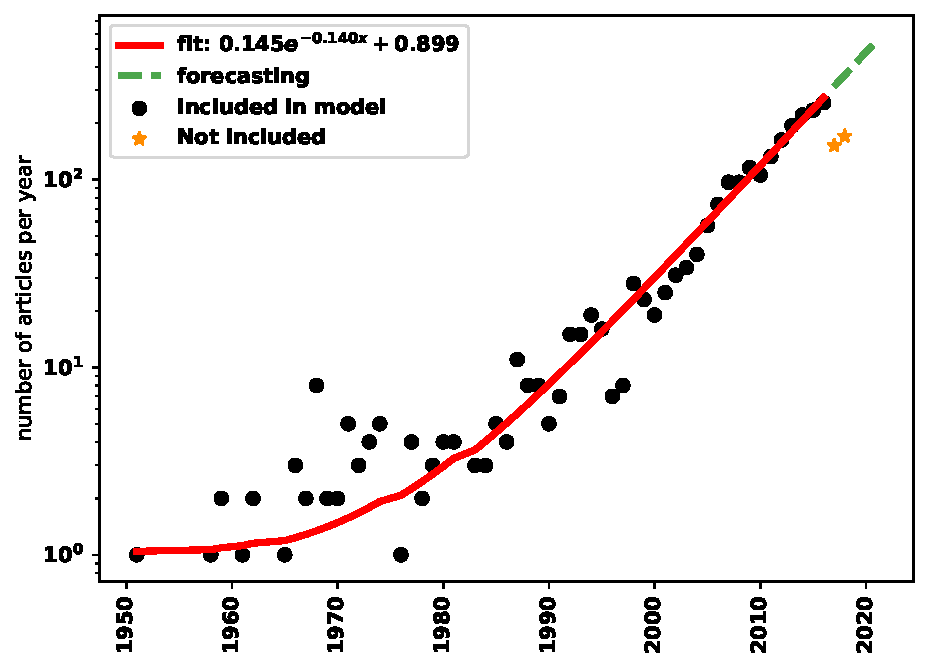
\includegraphics[width=.50\textwidth]{src/chapters/03/paper/bibliometric-study-of-the-prisoners-dilemma/assets/images/forecasting.pdf}
    \caption{Number of articles published on the PD 1951-2018 (on a log scale),
    with a fitted exponential line, and a forecast for 2017-2022.}\label{fig:timeseries}
\end{figure}

There are a total of \authors authors in the data set and several of these
authors have had multiple publications collected from the data collection process.
The highest number of articles collected for an
author is 83 publications for Matjaz Perc. The distribution of the number of
papers per author is given by Figure~\ref{fig:num_papers_per_author}, and it can
be seen that Matjaz Perc is an outlier. More specifically, most authors have
1 to 6 publications in the data set.

\begin{figure}[!hbtp]
    \centering
    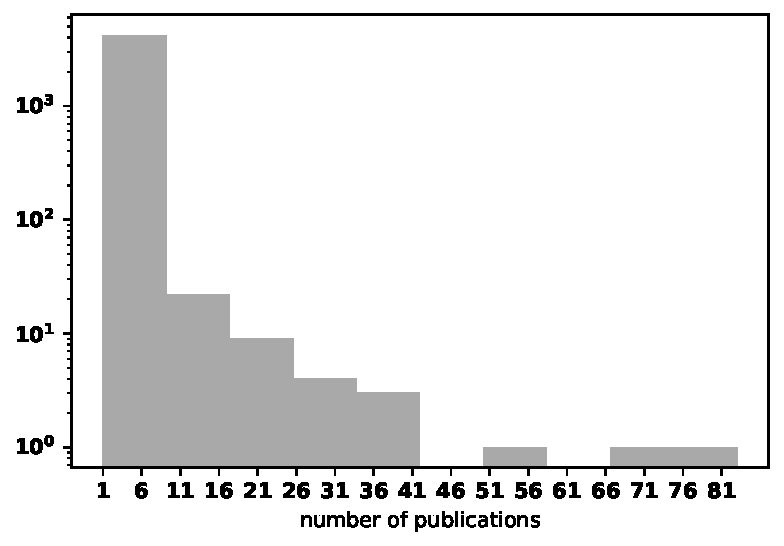
\includegraphics[width=.50\textwidth]{src/chapters/03/paper/bibliometric-study-of-the-prisoners-dilemma/assets/images/papers_per_author.pdf}
    \caption{Distribution of number of papers per author (on a log scale).}
    \label{fig:num_papers_per_author}
\end{figure}

The overall Collaboration Index (CI) or the average number of authors on
multi-authored papers is 3.2, thus on average a non single author publication in
the PD has 3 authors. This appears to be quite standard compared to other fields
such as cultural evolution~\cite{youngblood2018}, Astronomy and Astrophysics,
Genetics and Heredity, Nuclear and Particle Physics as reported
by~\cite{nature_author_blog}.
There are only a total of 545 publications with a single author, which
corresponds to the 22\% of the papers. It appears that academic publications
tend to be undertaken in the form of collaborative effort, which is in line
with the claim of~\cite{Kyvik2017}. From
Figure~\ref{fig:ci_over_time} the trend of CI over the years is given. There are
some peaks in the early years 1969 and 1980, however, a steady increase appears
to happen after 2004. This could be an effect of better communication tools
being introduced around that time which enabled more collaborations between
researchers.

\begin{figure}[!hbtp]
    \centering
    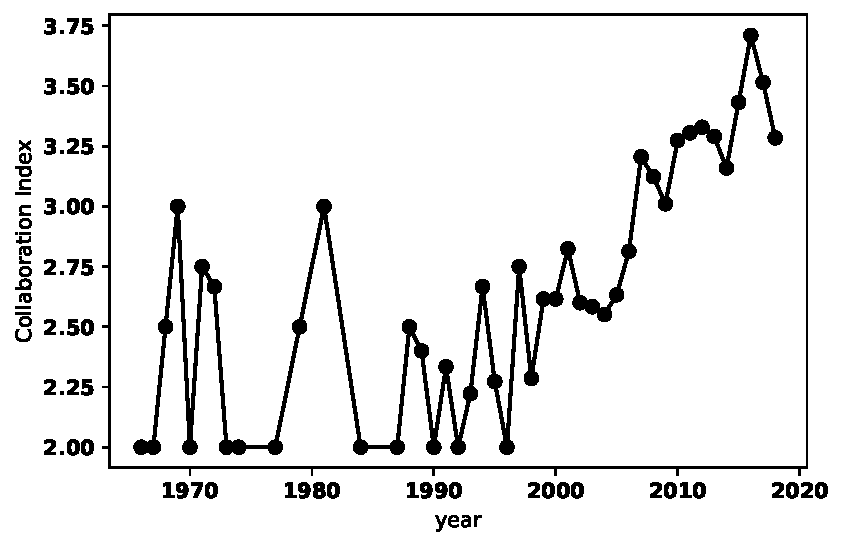
\includegraphics[width=.55\textwidth]{src/chapters/03/paper/bibliometric-study-of-the-prisoners-dilemma/assets/images/collaborative_index.pdf}
    \caption{Collaboration index over time.}\label{fig:ci_over_time}
\end{figure}

The collaborativeness of the authors is explored in more detail in
Section~\ref{section:co_authorship} using the co-authorship network. The
collaborative behaviour and relative influence of authors will also be explored
in co-authorship networks which correspond to their publications research topics.
These topics are presented in the next section.

\section{Research topics in the Prisoner's Dilemma research}\label{section:topics}

In order to identify the topics which are being discussed in the field of the
PD, the LDA algorithm implemented in~\cite{rehurek_lrec} is applied to the
abstracts of the data set. As mentioned before, the number of topics, which
will be denoted as \(n\), needs to be specified before running the algorithm.
The appropriate number of topics is chosen based on the coherence
value~\cite{Roder2015}. Figure~\ref{fig:coherence_value_over_number_of_topcis}
gives the coherence values of 18 models where \(n \in \{2, 3, \dots, 19\}\), and
it can be seen than the most appropriate number of topics is 6 with a coherence
value of 0.418.

\begin{figure}[!hbtp]
    \centering
    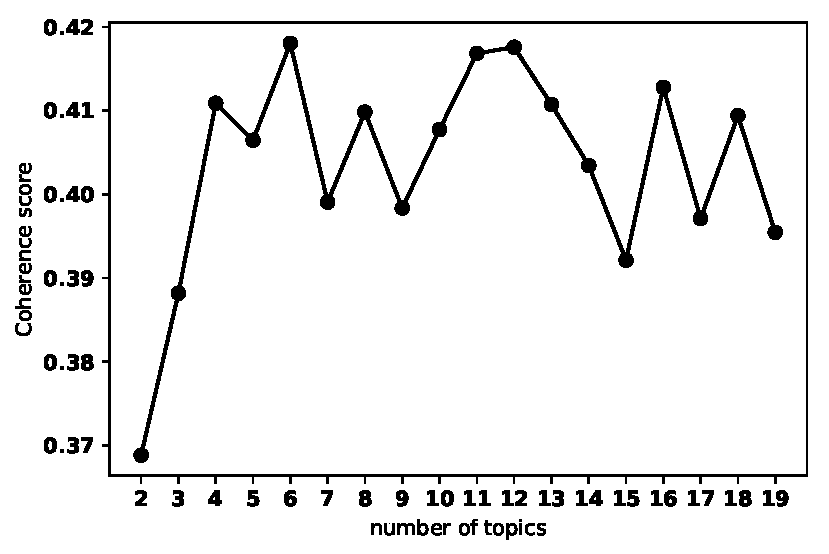
\includegraphics[width=.45\textwidth]{src/chapters/03/paper/bibliometric-study-of-the-prisoners-dilemma/assets/images/coherence_values.pdf}
    \caption{Coherence for LDA models over the number of topics.}
    \label{fig:coherence_value_over_number_of_topcis}
\end{figure}

The keywords associated with each topic for \(n=6\) are given by
Table~\ref{table:topics_keywords_n_6}. Though \(n=6\) has the highest coherence
score, from Table~\ref{table:topics_keywords_n_6} it can be observed that there
are overlapping keywords between the topics. Further manual investigation has
revealed that the seperation of topics are the most clear when an \(n\) of \(5\)
is considered. The LDA model for \(n=5\) has a coherence value 0.406 which is
close to 0.418 (the score for \(n=6\). Thus, \(n=5\) is chosen to carry out the analysis of this work.


\begin{table}[!hbtp]
    \begin{center}
    \resizebox{\textwidth}{!}{
    \begin{tabular}{lc}
\toprule
Topic & Topic Keywords \\
\midrule
A &                     model, theory, system, base, paper, problem, propose, present, approach, provide, analysis, framework, method, develop, solution \\
B &          \textcolor{red}{behavior}, \textcolor{red}{social}, human, decision, study, experiment, make, suggest, result, behaviour, effect, partner, participant, subject, experimental \\
C &                         individual, group, good, \textcolor{red}{social}, punishment, level, cost, mechanism, dilemma, cooperative, show, base, public, high, society \\
D &                          game, strategy, player, agent, play, dilemma, state, prisoner, payoff, equilibrium, result, iterate, set, probability, show \\
E &         population, evolutionary, dynamic, model, selection, result, evolution, evolve, show, process, size, \textcolor{red}{interaction}, \textcolor{red}{cooperator}, change, system \\
F &  cooperation, network, \textcolor{red}{interaction}, structure, study, evolution, find, \textcolor{red}{behavior}, cooperative, simulation, rule, spatial, \textcolor{red}{cooperator}, promote, result \\
\bottomrule
\end{tabular}
}
    \end{center}
    \caption{Keywords for each topic when \(n=6\). The highlighted keywords are overlapping keywords between topics.}
    \label{table:topics_keywords_n_6}
\end{table}

For \(n=5\) the articles are clustered and assigned to their dominant topic,
based on the highest percentage contribution. The keywords associated with a
topic, the most representative article of the topic (based on the
percentage contribution) and its academic reference are given by
Table~\ref{table:topics_and_articles}. The topics are labelled as A, B, C, D and
E, and more specifically:

\begin{itemize}
    \item Based on the keywords associated with Topic A, and the most
    representative article, Topic A appears to be about \textbf{human subject
    research}. Several publications assigned to the topic study the PD by
    setting experiments and having human participants simulate the game
    instead of computer simulations. These articles include~\cite{Matsumoto2016}
    which showed that prosocial behaviour increased with the age of the
    participants,~\cite{Li20140} which studied the difference in cooperation
    between high-functioning autistic and typically developing
    children,~\cite{Molina2013} explored the gender effect in highschool
    students and~\cite{Bell2017} explored the effect of facial expressions of
    individuals.
    \item Though it is not immediate from the keywords associated with
    Topic B, investigating the papers assigned to the topic indicate that it
    is focused on \textbf{biological studies}. Papers assigned to the topic include
    papers which apply the PD to genetics~\cite{Santorelli2008, Sistrom2015}, to
    the study of tumours~\cite{archetti2013evolutionary, sartakhti2017} and
    viruses~\cite{turner1999prisoner}. Other works include how phenotype affinity
    can affect the emergence of cooperation~\cite{wu2019phenotype} and modelling
    bacterial communities as a spatial structured social dilemma.
    \item Based on the keywords and the most representative article Topic
    C appears to include publications on PD \textbf{strategies}. Publications
    in the topic include the introduction of new strategies~\cite{stewart2013extortion},
    the search of optimality in strategies~\cite{banerjee2007reaching} and the
    training of strategies~\cite{ishibuchi2011evolution} with different
    representation methods. Moreover, publications that study the evolutionary
    stability of strategies~\cite{Adami2013} and introduced methods
    of differentiating between them~\cite{Ashlock2008} are
    also assigned to C.
    \item The keywords associated with Topic D clearly show that the topic
    is focused on \textbf{evolutionary dynamics on networks}. Publications include
    \cite{ichinose2013robustness} which explored the robustness of cooperation
    on networks,~\cite{wang2012spatial} which studied the effect of a strategy's neighbourhood
    on the emergence of cooperation and~\cite{chen2016fixation} which explored
    the fixation probabilities of any two strategies is spatial
    structures.
    \item The publication assigned to Topic E are on \textbf{modelling problems
    as a PD game}. Though Topic B is also concerned with problems being formulated
    as a PD, it includes only biological problems. In comparison, the problems
    in Topic E include decision making in
    operational research~\cite{ormerod2010or}, information sharing among members
    in a virtual team~\cite{feng2008trilateral}, the measurement of influence
    in articles based on citations~\cite{hutchins2016relative} and the price
    spikes in electric power markets~\cite{Guan2002}, and not on biological studies.
\end{itemize}

\begin{table}[!hbtp]
    \begin{center}
    \resizebox{\textwidth}{!}{
    \begin{tabularx}{1.5\textwidth}{lXXl|cc}
\toprule
Dominant Topic &                                                                                                 Topic Keywords &                                                                                                                                    Most Representative Article Title &        Reference &  \# Documents &  \% Documents \\
\midrule
A &                 social, behavior, human, study, experiment, cooperative, cooperation, suggest, find, behaviour &                                                                                      Facing Aggression: Cues Differ for Female versus Male Faces &  \cite{Geniole2012} &                496.0 &                   0.2008 \\
B &                               individual, group, good, show, high, increase, punishment, cost, result, benefit &  Genomic and Gene-Expression Comparisons among Phage-Resistant Type-IV Pilus Mutants of Pseudomonas syringae pathovar phaseolicola &  \cite{Sistrom2015} &                309.0 &                   0.1251 \\
C &                             game, strategy, player, agent, dilemma, play, payoff, state, prisoner, equilibrium &                                                            Fingerprinting: Visualization and Automatic Analysis of Prisoner's Dilemma Strategies &  \cite{Sistrom2015} &                561.0 &                   0.2271 \\
D &  cooperation, network, population, evolutionary, evolution, interaction, dynamic, structure, cooperator, study &                                                   Influence of initial distributions on robust cooperation in evolutionary  Prisoner's Dilemma &     \cite{Chen2007} &                556.0 &                   0.2251 \\
E &                           model, theory, base, system, problem, paper, propose, information, provide, approach &                                                                          Gaming and price spikes in electric power markets and possible remedies &     \cite{Guan2002} &                548.0 &                   0.2219 \\
\bottomrule
\end{tabularx}
}
    \end{center}
    \caption{Keywords for each topic and the document with the most representative article for each topic.}
    \label{table:topics_and_articles}
\end{table}

Note that the whilst for the choice of 5 topics the actual clustering is not
subjective (the algorithm is determining the output) the interpretation above is.

Thus, the five topics in the PD publications identified by the data set of using an LDA
are:

 \begin{enumerate} 
    \item human subject research, 
    \item biological studies, 
    \item strategies, 
    \item evolutionary dynamics on networks, 
    \item modelling problems as a PD.
\end{enumerate}
These topics nicely
summarise the PD research. They highlight the interdisciplinarity of the field;
how it brings together applied modelling of real world situations (Topic B and E)
and more theoretical notions such as evolutionary dynamics and optimality of
strategies.

Figure~\ref{fig:number_of_articles_per_topic} gives the number of articles
per topic over time. The topics appear to have had a similar trend over the years,
with topics B and D having a later start. Following the introduction of a topic
the publications in that topic have been increasing. There is no decreasing
trend in any of the topics. All the topics have been publishing for years and
they still attract the interest of academics. Thus, there does not
seem to be any given topic more or less in fashion.

\begin{figure}[!hbtp]
    \centering
    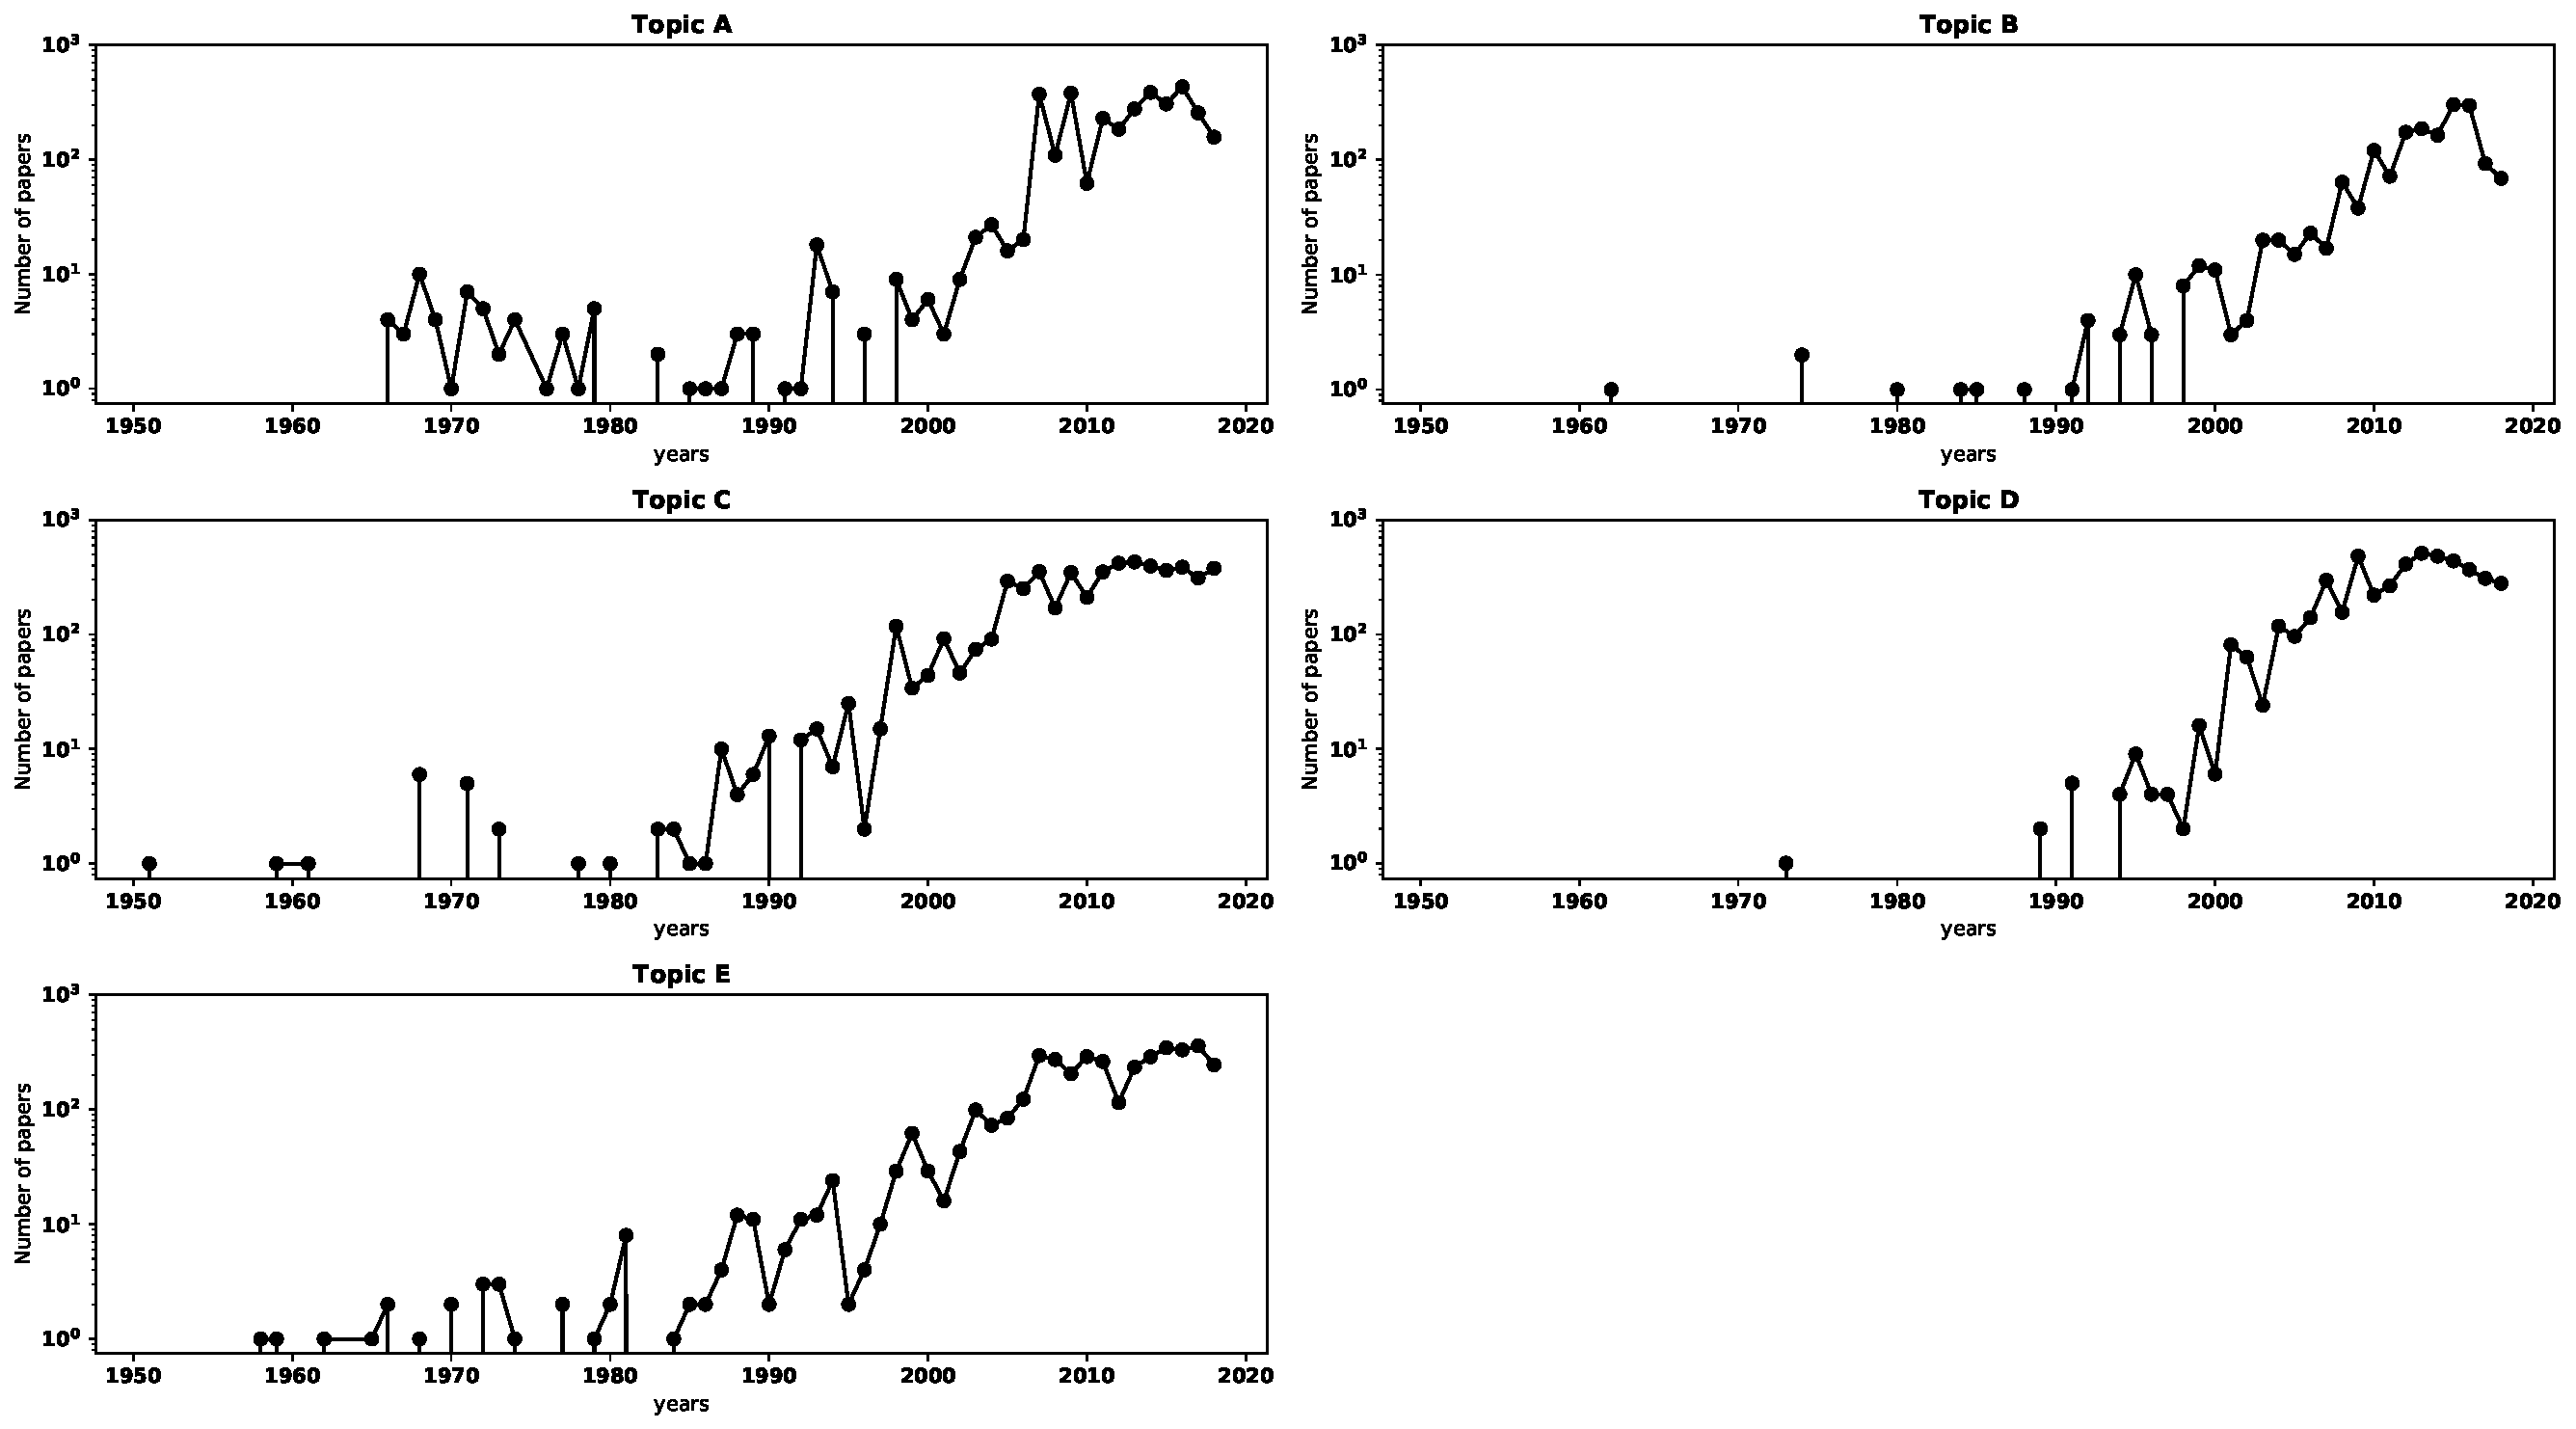
\includegraphics[width=\textwidth]{src/chapters/03/paper/bibliometric-study-of-the-prisoners-dilemma/assets/images/papers_per_topic_over_time.pdf}
    \caption{Number of articles per topic over the years (on a logged scale).}\label{fig:number_of_articles_per_topic}
\end{figure}

To gain a better understanding regarding the change in the topics over the years,
LDA is applied to the cumulative data set over 8 time periods. These periods are
1951-1965, 1951-1973, 1951-1980, 1951-1988, 1951-1995, 1951-2003, 1951-2010,
1951-2018. The number of topics for each cumulative subset is chosen based on
the coherence value and no objective approach is used. As a result, the period
1951-2018 has been assigned \(n=6\) which had the highest coherence
value instead of 5. The chosen models for each period including the
number of topics, their keywords and number of articles assigned to them are
given by Table \ref{table:topics_per_year}.

\begin{table}[!hbtp]
    \begin{center}
    \resizebox{\textwidth}{!}{
    \begin{tabular}{llccc}
\toprule
    Period &  Topic &                                                                                                Topic Keywords & Num of Documents & Percentage of Documents \\
\midrule
 1951-1965 &               1 &                 problem, technology, divert, euler, subsystem, requirement, trace, technique, system, untried &                3 &                   0.375 \\
 1951-1965 &               2 &            interpret, requirement, programme, evolution, article, increase, policy, system, trace, technology &                2 &                    0.25 \\
 1951-1965 &               3 &          equipment, agency, conjecture, development, untried, programme, trend, technology, weapon, technique &                1 &                   0.125 \\
 1951-1965 &               4 &                 variation, celebrated, trend, untried, change, involve, month, technique, subsystem, research &                1 &                   0.125 \\
 1951-1965 &               5 &                           give, good, modern, trace, technique, ambiguity, problem, trend, technology, system &                1 &                   0.125 \\
 \midrule
 1951-1973 &               1 &                           study, shock, cooperative, money, part, vary, investigate, good, receive, equipment &               12 &                  0.3243 \\
 1951-1973 &               2 &          cooperation, level, significantly, sequence, reward, provoke, descriptive, principal, display, argue &                4 &                  0.1081 \\
 1951-1973 &               3 &               player, make, effect, triad, experimental, motivation, dominate, hypothesis, instruction, trend &                3 &                  0.0811 \\
 1951-1973 &               4 &                                           ss, sex, male, female, dyad, design, suggest, college, factor, tend &                3 &                  0.0811 \\
 1951-1973 &               5 &               result, research, format, change, operational, analysis, relate, understanding, decision, money &                2 &                  0.0541 \\
 1951-1973 &               6 &                          condition, give, high, treatment, conflict, cc, real, original, replication, promote &                2 &                  0.0541 \\
 1951-1973 &               7 &              group, competitive, show, interpret, scale, compete, escalation, free, variable, individualistic &                2 &                  0.0541 \\
 1951-1973 &               8 &                        outcome, strategy, choice, type, pdg, difference, dummy, conclude, compare, consistent &                2 &                  0.0541 \\
 1951-1973 &               9 &                   game, difference, pair, approach, behavior, person, weapon, occur, advantaged, differential &                2 &                  0.0541 \\
 1951-1973 &              10 &                    response, present, dilemma, influence, cooperate, bias, point, amount, participate, factor &                2 &                  0.0541 \\
 1951-1973 &              11 &                       trial, problem, previous, involve, prisoner, experiment, follow, tit, increase, initial &                1 &                   0.027 \\
 1951-1973 &              12 &                           matrix, behavior, rational, black, model, research, broad, distance, complex, trace &                1 &                   0.027 \\
 1951-1973 &              13 &                    play, finding, individual, noncooperative, white, nature, race, ratio, represent, prisoner &                1 &                   0.027 \\
 \midrule
 1951-1980 &               1 &                                      play, trial, group, follow, white, interpret, scale, black, trend, small &               14 &                    0.25 \\
 1951-1980 &               2 &                              outcome, level, effect, type, dyad, vary, pdg, participate, understanding, arise &                9 &                  0.1607 \\
 1951-1980 &               3 &         game, strategy, cooperation, significant, difference, sentence, text, occur, differential, hypothesis &                4 &                  0.0714 \\
 1951-1980 &               4 &                        male, female, find, result, sex, subject, experimental, situation, treatment, computer &                4 &                  0.0714 \\
 1951-1980 &               5 &                         research, problem, influence, matrix, format, model, analysis, year, crime, equipment &                4 &                  0.0714 \\
 1951-1980 &               6 &                                    condition, dilemma, bias, free, attempt, book, year, dummy, prison, design &                4 &                  0.0714 \\
 1951-1980 &               7 &                    variable, result, factor, individual, ability, triad, half, migration, change, investigate &                3 &                  0.0536 \\
 1951-1980 &               8 &                 show, present, suggest, rational, compete, approach, characteristic, examine, person, conduct &                3 &                  0.0536 \\
 1951-1980 &               9 &                         behavior, high, finding, relate, obtain, assistance, ratio, good, weapon, competition &                3 &                  0.0536 \\
 1951-1980 &              10 &                               ss, shock, money, competitive, part, difference, pair, amount, man, information &                3 &                  0.0536 \\
 1951-1980 &              11 &             player, conflict, theory, decision, determine, produce, maker, cooperate, specialist, programming &                2 &                  0.0357 \\
 1951-1980 &              12 &            study, prisoner, make, response, experiment, noncooperative, standard, separate, conclude, initial &                2 &                  0.0357 \\
 1951-1980 &              13 &                       give, cooperative, choice, cognitive, real, operational, set, subject, ascribe, concern &                1 &                  0.0179 \\
 \midrule
 1951-1988 &               1 &                     trial, difference, find, choice, significant, competitive, effect, triad, interact, occur &               24 &                  0.2553 \\
 1951-1988 &               2 &                                            ss, shock, money, pair, response, part, high, tit, receive, amount &               13 &                  0.1383 \\
 1951-1988 &               3 &                         suggest, paper, case, debate, view, achieve, framework, natural, assumption, finitely &               10 &                  0.1064 \\
 1951-1988 &               4 &                     prisoner, dilemma, behavior, model, present, involve, person, increase, trust, experiment &                8 &                  0.0851 \\
 1951-1988 &               5 &                                   game, player, show, approach, repeat, previous, move, tat, related, include &                8 &                  0.0851 \\
 1951-1988 &               6 &                cooperation, level, mutual, equilibrium, standard, provide, information, human, real, question &                6 &                  0.0638 \\
 1951-1988 &               7 &                      play, result, male, subject, female, cooperative, sex, experimental, treatment, computer &                5 &                  0.0532 \\
 1951-1988 &               8 &                        research, study, variable, ability, factor, conflict, matrix, year, student, interpret &                4 &                  0.0426 \\
 1951-1988 &               9 &                                         problem, group, small, scale, social, issue, large, base, bias, party &                4 &                  0.0426 \\
 1951-1988 &              10 &                          game, strategy, outcome, type, cooperate, ethical, pdg, explain, dependent, separate &                4 &                  0.0426 \\
 1951-1988 &              11 &              give, condition, individual, major, dyad, behaviour, produce, conflict, assistance, collectively &                3 &                  0.0319 \\
 1951-1988 &              12 &                        situation, iterate, statement, rational, card, side, paradox, true, consequence, front &                2 &                  0.0213 \\
 1951-1988 &              13 &                               inflation, hypothesis, rate, run, change, demand, nominal, cost, output, growth &                2 &                  0.0213 \\
 1951-1988 &              14 &                                     theory, make, analysis, decision, system, examine, work, soft, lead, hard &                1 &                  0.0106 \\
 \midrule
 1951-1995 &               1 &                            strategy, population, evolution, iterate, tit, opponent, evolve, dynamic, set, tat &               31 &                  0.1732 \\
 1951-1995 &               2 &                 game, repeat, assumption, rule, person, equilibrium, general, finitely, indefinitely, analyze &               24 &                  0.1341 \\
 1951-1995 &               3 &                            inflation, long, rate, hypothesis, run, policy, cost, nominal, demand, programming &               20 &                  0.1117 \\
 1951-1995 &               4 &            condition, outcome, trial, find, difference, cooperation, experiment, level, significant, response &               15 &                  0.0838 \\
 1951-1995 &               5 &                     rational, result, receive, statement, money, paradox, shock, iterate, consequence, common &               14 &                  0.0782 \\
 1951-1995 &               6 &             cooperation, show, competitive, high, probability, conflict, simulation, altruism, yield, natural &               14 &                  0.0782 \\
 1951-1995 &               7 &                           prisoner, dilemma, give, point, defect, form, cooperator, increase, relate, ethical &               10 &                  0.0559 \\
 1951-1995 &               8 &                       player, give, decision, provide, cooperative, game, previous, pair, determine, interact &                9 &                  0.0503 \\
 1951-1995 &               9 &                          play, cooperate, result, male, subject, female, time, relationship, suggest, student &                8 &                  0.0447 \\
 1951-1995 &              10 &                                   problem, group, theory, good, approach, society, large, scale, issue, level &                8 &                  0.0447 \\
 1951-1995 &              11 &            study, situation, behaviour, computer, argue, change, implication, characteristic, real, associate &                8 &                  0.0447 \\
 1951-1995 &              12 &                        model, paper, behavior, examine, present, mutual, expectation, develop, type, variable &                7 &                  0.0391 \\
 1951-1995 &              13 &                                   make, research, system, analysis, choice, work, base, relation, world, wide &                6 &                  0.0335 \\
 1951-1995 &              14 &               individual, social, behavior, standard, choose, evolutionary, partner, payoff, defection, small &                5 &                  0.0279 \\
 \midrule
 1951-2003 &               1 &                                    game, player, dilemma, prisoner, theory, give, paper, make, group, problem &              151 &                  0.4266 \\
 1951-2003 &               2 &                         cooperation, result, play, show, cooperate, condition, cooperative, high, level, time &              106 &                  0.2994 \\
 1951-2003 &               3 &                  strategy, model, agent, study, behavior, individual, population, evolutionary, state, player &               97 &                   0.274 \\
 \midrule
 1951-2010 &               1 &                                  model, theory, paper, base, make, present, problem, provide, human, decision &              325 &                  0.3454 \\
 1951-2010 &               2 &                                   game, strategy, player, agent, play, dilemma, system, behavior, show, state &              322 &                  0.3422 \\
 1951-2010 &               3 &  cooperation, network, study, population, individual, evolutionary, social, evolution, interaction, structure &              294 &                  0.3124 \\
 \midrule
 1951-2018 &               1 &                              model, theory, system, base, paper, problem, propose, present, approach, provide &              556 &                  0.2251 \\
 1951-2018 &               2 &                        behavior, social, human, decision, study, experiment, make, suggest, result, behaviour &              482 &                  0.1951 \\
 1951-2018 &               3 &                     individual, group, good, social, punishment, level, cost, mechanism, dilemma, cooperative &              428 &                  0.1733 \\
 1951-2018 &               4 &                            game, strategy, player, agent, play, dilemma, state, prisoner, payoff, equilibrium &              380 &                  0.1538 \\
 1951-2018 &               5 &                 population, evolutionary, dynamic, model, selection, result, evolution, evolve, show, process &              351 &                  0.1421 \\
 1951-2018 &               6 &       cooperation, network, interaction, structure, study, evolution, find, behavior, cooperative, simulation &              273 &                  0.1105 \\
\bottomrule
\end{tabular}
}
    \end{center}
    \caption{Topic modelling result for the cumulative data set over the periods
    }\label{table:topics_per_year}
\end{table}

But how well do the five topics which were presented earlier fit the
publications over time? This is answered by comparing the performance of three
LDA models over the cumulative periods' publications. The three models are LDA
models for the entire data set for \(n\) equal to 5, 6 and the optimal number of topics over time. For
each model the \(c^*\) is estimated for each document in the cumulative data
sets. The performance of the models are then compared based on:

\begin{equation}\label{eq:ratio}
    \bar{c^*} \times n
\end{equation}

where \(\bar{c^*}\) is the median highest percentage contribution and \(n\)
is the number of topics of a given period. A model with more topics will have more
difficulty to assign papers. Thus, equation (ref{eq:ratio}) is a measure of confidence
in assigning a given paper to its topic weighted by the number of topics.
The performances are
given by Figure~\ref{fig:median_percentage_contribution_over_time}.

The five topics of the PD presented in this manuscript appear to always be
less good at fitting the publications compared to the six topics of LDA \(n=6\).
Moreover, there are less good than the topics of the optimal number of topics
from 1951 to 1995. The difference in the performance values, equation (\ref{eq:ratio}),
however are small. The relevances of the five topics has been increasing
over time, and though, the topics did not always fit the majority of published
work over time, there were still papers being published on those topics.

\begin{figure}[!hbtp]
    \centering
    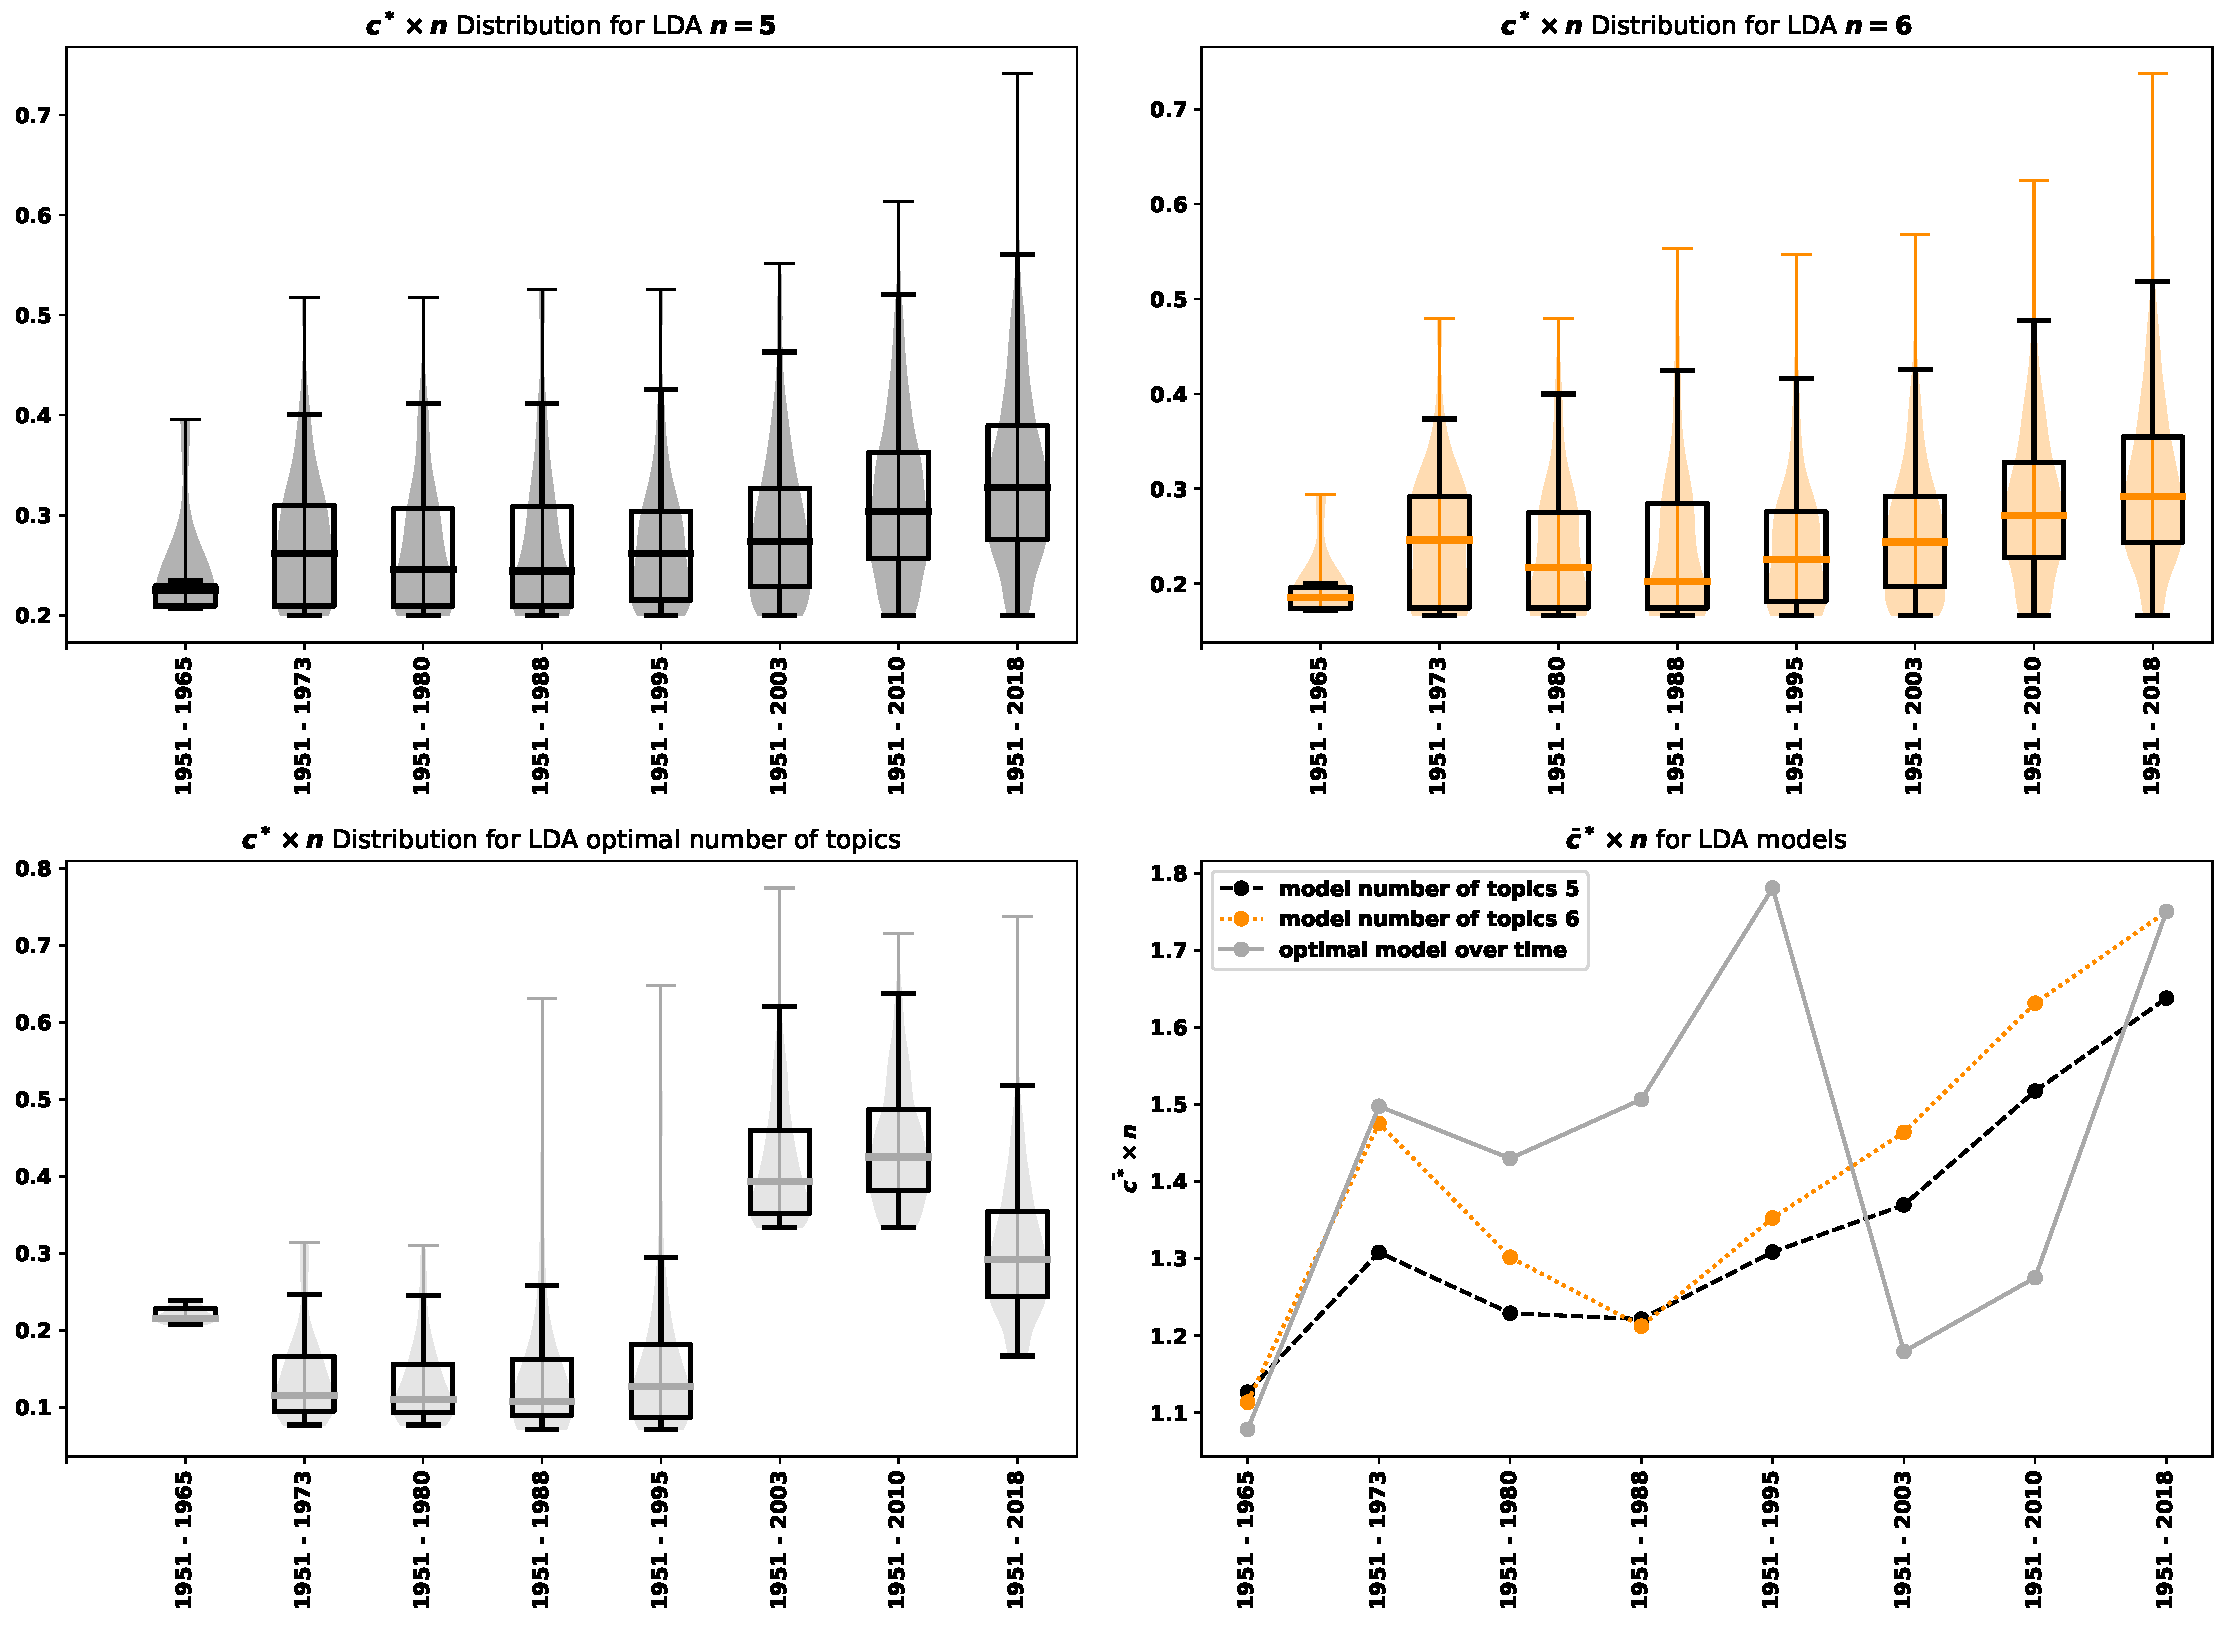
\includegraphics[width=.75\textwidth]{src/chapters/03/paper/bibliometric-study-of-the-prisoners-dilemma/assets/images/contribution_over_time.pdf}
    \caption{Maximum percentage contributions (\(c^*\)) over the time periods,
    for the LDA models for the entire data set for \(n\) equal to 5, 6
    and the optimal number of topics over time.}
    \label{fig:median_percentage_contribution_over_time}
\end{figure}

In the following section the collaborative behaviour of authors in the field,
and within the field's topics as were presented in this section, are explored
using a network theoretic approach.

\section{Analysis of co-authorship network}\label{section:co_authorship}

The collaborative behaviour of authors in the field of the PD is assessed using
the co-authorship network, which as introduced in
section~\ref{section:methodology} is denoted as \(G\). There are a total of
\connectedcomponents connected components in \(G\) and the largest component has
a size of \largestcc nodes. The largest connected component is going to be
refereed to as the main cluster of the network and is denoted as \(\bar{G}\). A
graphical representation of both networks is shown in
Figures~\ref{fig:graphical_representation_g}-\ref{fig:graphical_representation_g_bar}
and a metrics summary is given by Table~\ref{table:network_comparison.tex}.

\begin{figure}[!hbtp]
    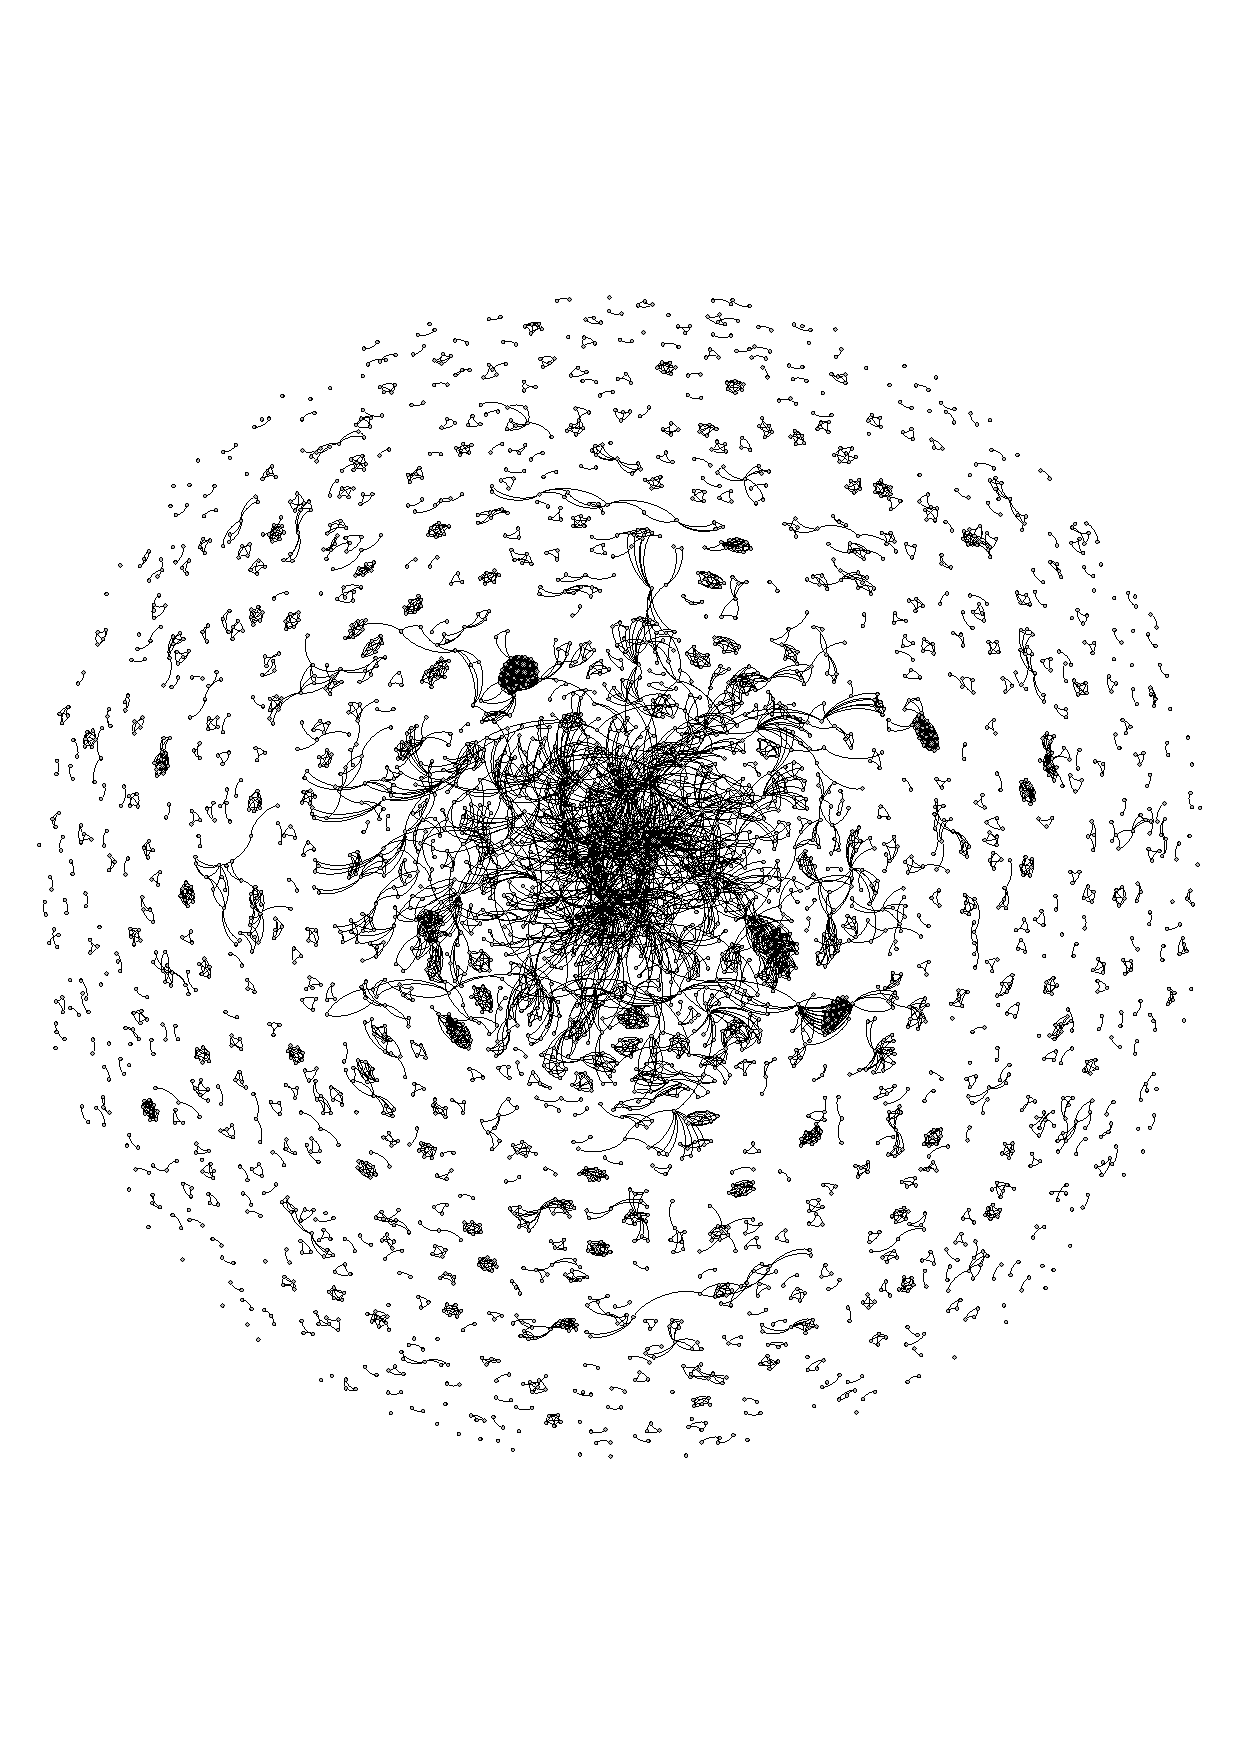
\includegraphics[width=\textwidth]{src/chapters/03/paper/bibliometric-study-of-the-prisoners-dilemma/assets/images/pd_network.pdf}
    \caption{\(G\) the co-authorship network for the IPD.}\label{fig:graphical_representation_g}
\end{figure}

\begin{figure}[!hbtp]
    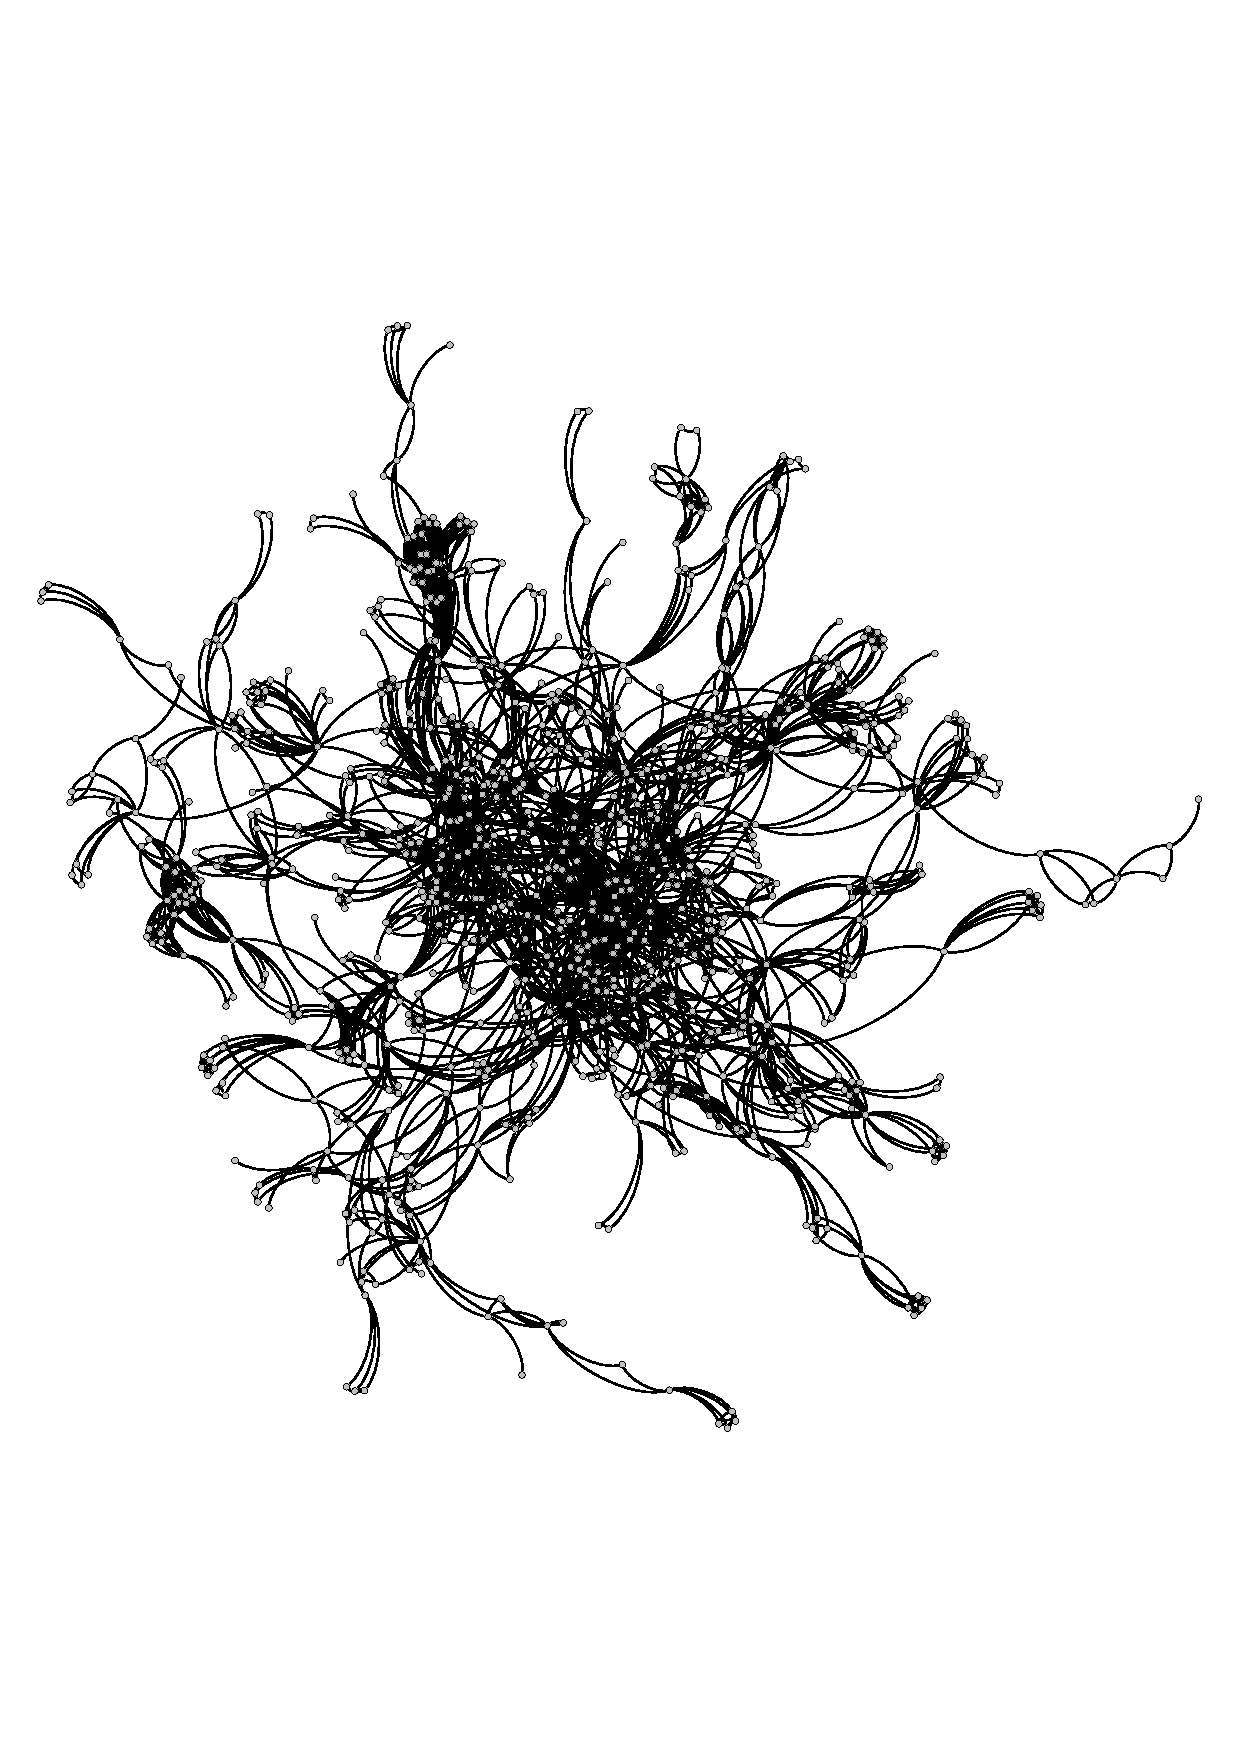
\includegraphics[width=\textwidth]{src/chapters/03/paper/bibliometric-study-of-the-prisoners-dilemma/assets/images/pd_network_cluster.pdf}
    \caption{\(\bar{G}\) the largest connected component of \(G\).}\label{fig:graphical_representation_g_bar}
\end{figure}

Based on Table~\ref{table:network_comparison.tex} an author in \(G\) has on
average 4 collaborators and a 70\% probability of collaborating with a
collaborator's co-author. An author of \(\bar{G}\) on average is 7\% more likely
to write with a collaborator's co-author and on average has 2 more
collaborators. Moreover, there are only \isolatedpercentage\% of authors in the
PD that has no connection to any other author.

\begin{table}[!hbtp]
    \centering
    \resizebox{\textwidth}{!}{
    \begin{tabular}{lrrrrrrrrrr}
\toprule
{} &  \# Nodes &  \# Edges  &  \% Isolated nodes &  \# Connected components &  Size of largest component &  Av. degree &  \# Communities &  Modularity &  Clustering coeff \\
\midrule
$G$       &     4011 &     7642 &               3.2 &                     947 &                        796 &       3.811 &            967 &     0.96491 &             0.701 \\
$\bar{G}$ &      796 &     2214 &               0.0 &                       1 &                        796 &       5.563 &             25 &     0.84406 &             0.773 \\
\bottomrule
\end{tabular}
}
    \caption{Network metrics for \(G\) and \(\bar{G}\) respectively.}
    \label{table:network_comparison.tex}
\end{table}

But how do these compare to other fields? Two more data sets for the topics
``Price of Anarchy'' and ``Auction Games'' have been collected in order to
compare the collaborative behaviour of the PD to other game theoretic fields. A
total of 3444 publications have been collected for Auction games and 748 for
Price of Anarchy. Price of Anarchy is relatively a new field, with the first
publication on the topic being~\cite{Koutsoupias1999} in 1999. This explains the
small number of articles that have been retrieved. Both data sets have been
archived and are available in~\cite{auction_data_2018, anarchy_data_2018}.
The networks for both data sets have been generated in the same way as \(G\).
A summary of the networks' metrics are given by Table~\ref{table:other_topics_network_comparison.tex}.

\begin{table}[!hbtp]
    \centering
    \resizebox{\textwidth}{!}{
    \begin{tabular}{lrrrrP{0.2\textwidth}P{0.2\textwidth}rrrrr}
\toprule
{} &  \# Nodes &  \# Edges &  \# Isolated nodes &  \% Isolated nodes &  \# Connected components &  Size of largest component &  Av. degree &  \# Communities &  Modularity &  Clustering coeff \\
\midrule
auction Games    &     5165 &     7861 &               256 &               5.0 &                    1272 &                       1348 &       3.044 &           1294 &       0.957 &             0.622 \\
price of Anarchy &     1155 &     1953 &                 4 &               0.3 &                     245 &                        222 &       3.382 &            253 &       0.965 &             0.712 \\
\bottomrule
\end{tabular}
}
    \caption{Network metrics for auction games and price of anarchy networks respectively.}
    \label{table:other_topics_network_comparison.tex}
\end{table}

The average degrees for the Price of Anarchy and for Auction games are lower
than the PD's. In Auction games an author is more likely to have no collaborators,
and in the Price of Anarchy there are almost no authors that are not connected
to someone. This could be an effect of the field being introduced in more modern
days. Overall, an author in the PD has on average more collaborators
and there are less isolated authors compared to another well established game
theoretic field. These results seem to indicate that the PD is a \textit{relatively} collaborative
field.

However, both \(G\) and \(\bar{G}\) have a high modularity (larger than 0.84) and a large number of
communities (967 and 25 respectively). A high modularity implies that authors create their own publishing
communities but not many publications from authors from different communities
occur. Thus, author tends to collaborate with authors in their communities but
not many efforts are made to create new connections to other communities and
spread the knowledge of the field across academic teams. The fields
of both Price of Anarchy and Auction games also have high modularity, and
that could indicate that is in fact how academic publications are.
Thus, the PD is indeed a collaborative field but perhaps it is not
more collaborative than other fields, as there is no effort from the authors
to write with people outside their community.

The evolution of the networks was also explored over time by constructing the
network cumulatively over 51 periods. Except from the first period 1951-1966 the
rest of the periods have a yearly interval (data for the years 1975 and 1982
were not retrieved by the collection data process). The metrics of each sub
network are given by Tables~\ref{table:cumulative_graphs} and~\ref{table:cumulative_clusters}.

\begin{table}[!hbtp]
    \centering
    \resizebox{.9\textwidth}{!}{
    \begin{tabular}{lrrrrrrrrrr}
\toprule
Period &  \# Nodes &  \# Edges &  \% Isolated nodes &  \multicolumn{1}{p{3cm}}{\centering Size of largest component} &  Av. degree &  \# Communities &  Modularity &  Clustering coeff \\
\midrule
1951 - 1966 &        2 &        1 &    0.0 &     2 &       1.000 &              1 &       0.000 &             0.000 \\
1951 - 1967 &        2 &        1 &    0.0 &     2 &       1.000 &              1 &       0.000 &             0.000 \\
1951 - 1968 &        5 &        8 &    0.0 &     5 &       3.200 &              1 &       0.000 &             0.867 \\
1951 - 2002 &        7 &       21 &    0.0 &     7 &       6.000 &              1 &       0.000 &             1.000 \\
1951 - 2003 &        7 &       21 &    0.0 &     7 &       6.000 &              1 &       0.000 &             1.000 \\
1951 - 2004 &       10 &       13 &    0.0 &    10 &       2.600 &              2 &       0.376 &             0.553 \\
1951 - 2005 &       19 &       28 &    0.0 &    19 &       2.947 &              3 &       0.544 &             0.730 \\
1951 - 2006 &       22 &       35 &    0.0 &    22 &       3.182 &              4 &       0.527 &             0.720 \\
1951 - 2007 &       25 &       39 &    0.0 &    25 &       3.120 &              5 &       0.558 &             0.686 \\
1951 - 2008 &       33 &       62 &    0.0 &    33 &       3.758 &              4 &       0.623 &             0.736 \\
1951 - 2009 &       71 &      148 &    0.0 &    71 &       4.169 &              6 &       0.697 &             0.698 \\
1951 - 2010 &      133 &      387 &    0.0 &   133 &       5.820 &              7 &       0.726 &             0.749 \\
1951 - 2011 &      157 &      465 &    0.0 &   157 &       5.924 &              8 &       0.727 &             0.725 \\
1951 - 2012 &      209 &      611 &    0.0 &   209 &       5.847 &             11 &       0.733 &             0.737 \\
1951 - 2013 &      322 &      892 &    0.0 &   322 &       5.540 &             12 &       0.780 &             0.743 \\
1951 - 2014 &      399 &     1109 &    0.0 &   399 &       5.559 &             15 &       0.794 &             0.742 \\
1951 - 2015 &      504 &     1368 &    0.0 &   504 &       5.429 &             24 &       0.811 &             0.751 \\
1951 - 2016 &      613 &     1677 &    0.0 &   613 &       5.471 &             21 &       0.819 &             0.761 \\
1951 - 2017 &      706 &     1935 &    0.0 &   706 &       5.482 &             29 &       0.830 &             0.772 \\
1951 - 2018 &      796 &     2214 &    0.0 &   796 &       5.563 &             25 &       0.845 &             0.773 \\
\bottomrule
\end{tabular}
}
    \caption{Collaborativeness metrics for cumulative graphs' main clusters, \(\tilde{G} \subseteq \bar{G}\)}\label{table:cumulative_clusters}
\end{table}

\begin{table}[!hbtp]
    \centering
    \resizebox{\textwidth}{!}{
    \begin{tabular}{lrrrrrrrrrr}
\toprule
Period &  \# Nodes &  \# Edges &  \% Isolated nodes &  \multicolumn{1}{p{3cm}}{\centering \# Connected components} &  \multicolumn{1}{p{3cm}}{\centering Size of largest component} &  Av. degree &  \# Communities &  Modularity &  Clustering coeff \\
\midrule
1951 - 1966 &        6 &        3 &    0.0 &                       3 &                          2 &       1.000 &              3 &       0.667 &             0.000 \\
1951 - 1967 &        8 &        4 &    0.0 &                       4 &                          2 &       1.000 &              4 &       0.750 &             0.000 \\
1951 - 1968 &       19 &       15 &    0.0 &                       8 &                          5 &       1.579 &              8 &       0.684 &             0.228 \\
1951 - 1969 &       20 &       17 &    0.0 &                       8 &                          6 &       1.700 &              8 &       0.630 &             0.250 \\
1951 - 1970 &       22 &       18 &    0.0 &                       9 &                          6 &       1.636 &              9 &       0.667 &             0.227 \\
1951 - 1971 &       33 &       28 &    0.0 &                      13 &                          6 &       1.697 &             13 &       0.827 &             0.424 \\
1951 - 1972 &       39 &       34 &    0.0 &                      15 &                          6 &       1.744 &             15 &       0.867 &             0.513 \\
1951 - 1973 &       42 &       35 &    2.4 &                      17 &                          6 &       1.667 &             17 &       0.873 &             0.476 \\
1951 - 1974 &       42 &       35 &    2.4 &                      17 &                          6 &       1.667 &             17 &       0.873 &             0.476 \\
1951 - 1976 &       42 &       35 &    2.4 &                      17 &                          6 &       1.667 &             17 &       0.873 &             0.476 \\
1951 - 1977 &       44 &       36 &    2.3 &                      18 &                          6 &       1.636 &             18 &       0.880 &             0.455 \\
1951 - 1978 &       44 &       36 &    2.3 &                      18 &                          6 &       1.636 &             18 &       0.880 &             0.455 \\
1951 - 1979 &       47 &       40 &    2.1 &                      18 &                          6 &       1.702 &             18 &       0.884 &             0.454 \\
1951 - 1980 &       47 &       40 &    2.1 &                      18 &                          6 &       1.702 &             18 &       0.884 &             0.454 \\
1951 - 1981 &       50 &       46 &    2.0 &                      18 &                          6 &       1.840 &             18 &       0.889 &             0.497 \\
1951 - 1983 &       51 &       46 &    3.9 &                      19 &                          6 &       1.804 &             19 &       0.889 &             0.487 \\
1951 - 1984 &       53 &       47 &    3.8 &                      20 &                          6 &       1.774 &             20 &       0.894 &             0.469 \\
1951 - 1985 &       53 &       47 &    3.8 &                      20 &                          6 &       1.774 &             20 &       0.894 &             0.469 \\
1951 - 1986 &       53 &       47 &    3.8 &                      20 &                          6 &       1.774 &             20 &       0.894 &             0.469 \\
1951 - 1987 &       56 &       48 &    5.4 &                      22 &                          6 &       1.714 &             22 &       0.898 &             0.443 \\
1951 - 1988 &       62 &       52 &    6.5 &                      25 &                          6 &       1.677 &             25 &       0.909 &             0.449 \\
1951 - 1989 &       75 &       62 &    6.7 &                      31 &                          6 &       1.653 &             31 &       0.926 &             0.424 \\
1951 - 1990 &       79 &       64 &    6.3 &                      33 &                          6 &       1.620 &             33 &       0.930 &             0.403 \\
1951 - 1991 &       87 &       69 &    6.9 &                      37 &                          6 &       1.586 &             37 &       0.937 &             0.400 \\
1951 - 1992 &       95 &       72 &   10.5 &                      42 &                          6 &       1.516 &             42 &       0.941 &             0.367 \\
1951 - 1993 &      106 &       81 &   11.3 &                      47 &                          6 &       1.528 &             47 &       0.947 &             0.366 \\
1951 - 1994 &      124 &       95 &   12.9 &                      56 &                          6 &       1.532 &             56 &       0.955 &             0.394 \\
1951 - 1995 &      135 &      102 &   12.6 &                      61 &                          6 &       1.511 &             61 &       0.960 &             0.384 \\
1951 - 1996 &      142 &      105 &   12.7 &                      65 &                          6 &       1.479 &             65 &       0.962 &             0.365 \\
1951 - 1997 &      155 &      115 &   12.9 &                      71 &                          6 &       1.484 &             71 &       0.966 &             0.392 \\
1951 - 1998 &      191 &      140 &   11.0 &                      87 &                          6 &       1.466 &             87 &       0.973 &             0.367 \\
1951 - 1999 &      221 &      169 &   11.3 &                      99 &                          6 &       1.529 &             99 &       0.977 &             0.397 \\
1951 - 2000 &      250 &      195 &   10.8 &                     110 &                          6 &       1.560 &            110 &       0.979 &             0.418 \\
1951 - 2001 &      287 &      235 &   10.5 &                     125 &                          7 &       1.638 &            125 &       0.977 &             0.419 \\
1951 - 2002 &      335 &      278 &   10.7 &                     146 &                          7 &       1.660 &            146 &       0.979 &             0.428 \\
1951 - 2003 &      381 &      310 &   10.5 &                     168 &                          7 &       1.627 &            168 &       0.982 &             0.413 \\
1951 - 2004 &      437 &      370 &    9.2 &                     185 &                         10 &       1.693 &            185 &       0.983 &             0.424 \\
1951 - 2005 &      532 &      476 &    7.7 &                     214 &                         19 &       1.789 &            214 &       0.985 &             0.458 \\
1951 - 2006 &      640 &      603 &    6.7 &                     246 &                         22 &       1.884 &            246 &       0.987 &             0.486 \\
1951 - 2007 &      793 &      877 &    5.8 &                     283 &                         25 &       2.212 &            283 &       0.985 &             0.532 \\
1951 - 2008 &      948 &     1170 &    5.3 &                     318 &                         33 &       2.468 &            319 &       0.985 &             0.558 \\
1951 - 2009 &     1108 &     1442 &    4.9 &                     356 &                         71 &       2.603 &            358 &       0.982 &             0.573 \\
1951 - 2010 &     1300 &     1936 &    5.1 &                     402 &                        133 &       2.978 &            405 &       0.965 &             0.592 \\
1951 - 2011 &     1560 &     2375 &    5.1 &                     472 &                        157 &       3.045 &            475 &       0.970 &             0.613 \\
1951 - 2012 &     1837 &     2865 &    4.4 &                     534 &                        209 &       3.119 &            537 &       0.969 &             0.634 \\
1951 - 2013 &     2149 &     3420 &    4.3 &                     603 &                        322 &       3.183 &            609 &       0.965 &             0.644 \\
1951 - 2014 &     2481 &     3971 &    4.2 &                     683 &                        399 &       3.201 &            694 &       0.962 &             0.658 \\
1951 - 2015 &     2938 &     4877 &    3.7 &                     765 &                        504 &       3.320 &            779 &       0.965 &             0.675 \\
1951 - 2016 &     3469 &     6532 &    3.3 &                     850 &                        613 &       3.766 &            863 &       0.964 &             0.696 \\
1951 - 2017 &     3735 &     7072 &    3.2 &                     895 &                        706 &       3.787 &            912 &       0.964 &             0.700 \\
1951 - 2018 &     4011 &     7642 &    3.2 &                     947 &                        796 &       3.811 &            967 &       0.966 &             0.701 \\
\bottomrule
\end{tabular}
}
    \caption{Collaborativeness metrics for cumulative graphs, \(\tilde{G} \subseteq G\)}\label{table:cumulative_graphs}
\end{table}

The results, similarly to the results of~\cite{Liu2015}, confirm that the
networks grow over time and that the networks always had a high modularity.
Since the first publications authors tend to write with people from their
communities, and that is not an effect of a specific time period.

The networks corresponding to the topics of Section~\ref{section:preliminary} have
also been generated similarly to \(G\). Note that authors with publications in
more than one topic exist, and these authors are included in all the corresponding
networks. A metrics' summary for all five topic networks is given by Table
\ref{table:topics_networks}.

\begin{table}[!hbtp]
    \centering
    \resizebox{\textwidth}{!}{
    \begin{tabular}{lrrrrrrrrrr}
\toprule
{} &  \# Nodes &  \# Edges &  \# Isolated nodes &  \% Isolated nodes &  \# Connected components &  Size of largest component &  Av. degree &  \# Communities &  Modularity &  Clustering coeff \\
\midrule
Topic A &     1124 &     2137 &                15 &               1.3 &                     264 &                         56 &       3.802 &            265 &       0.983 &             0.759 \\
Topic B &      695 &     1382 &                13 &               1.9 &                     157 &                         80 &       3.977 &            158 &       0.950 &             0.773 \\
Topic C &      900 &     1141 &                41 &               4.6 &                     281 &                         29 &       2.536 &            281 &       0.981 &             0.636 \\
Topic D &      880 &     1509 &                17 &               1.9 &                     174 &                        312 &       3.430 &            183 &       0.918 &             0.701 \\
Topic E &     1045 &     1964 &                59 &               5.6 &                     354 &                         31 &       3.759 &            354 &       0.926 &             0.664 \\
\bottomrule
\end{tabular}
}
    \caption{Network metrics for topic networks.}\label{table:topics_networks}
\end{table}

Topic B is the network with the highest average degree followed by Topic A. The
topic with the smallest average degree, 2.5, is Topic C. In topics A and B the
number of isolated nodes is very small \(less than (0.2)\) compared to Topic E where the
percentage of isolated nodes is approximately 6\%. Moreover, in topics C and E
an author is 10\% more likely to collaborate with a collaborator's co-author.
Thus, topics ``human subject research'' and ``biological studies'' tend
to be more collaborative than the topic of ``strategies'', and an authors in
these are less likely to have at least one collaborator compared to the topic of
``modelling problems as a PD''.

``Evolutionary dynamics on networks'' also appear to be a collaborative topic.
In fact the network of the topic  is a
sub graph of \(\bar{G}\), the main cluster of \(G\) and it will be demonstrated in the following section that
authors in this network are more like to gain from the influence of the network
compared to any other topic network.

The two centrality measures reported in this thesis are closeness and
betweenness centrality. Closeness centrality is a measure of how easy it is for
an author to contact others, and consequently affect them; influence them. Thus
closeness centrality is a measure of influence. Betweenness centrality is a
measure of how many paths pass through a specific node, thus the amount of
information this person has access to. Betweenness centrality is interpreted as a
measure of how much an author gains from the field. The values of the centralities
can range between 0 and 1. Influence and the amount of information
an author has access to are proxies to understand if/which authors benefit more
from their position.

For \(G\) and \(\bar{G}\) the most central authors based on closeness and
betweenness centralities are given by Table~\ref{table:central_authors}. The
most central authors in \(G\) and \(\bar{G}\) are the same. This implies that
the results on centrality heavily rely on the main cluster (as expected). Matjaz Perc is an
author with 83 publications in the data set and the most central authors based
on both centrality measures. The most central authors are fairly similar between
the two measures. The author that appear to be central based on one measure and
not the other are Martin Nowak, Franz Weissing, Jianye Hao, Angel Sanchez and
Valerio Capraro which have access to information due to their
positioning but do not influence the network as much, and the opposite is true
for Attila Szolnoki, Luo-Luo Jiang Sandro Meloni, Cheng-Yi Xia and Xiaojie Chen.

\begin{table}[!hbtp]
    \begin{center}
    \resizebox{.9\textwidth}{!}{\begin{tabular}{lgrgr|grgr}
\toprule
& \multicolumn{4}{c}{$G$} & \multicolumn{4}{c}{$\bar{G}$} \\
\midrule
{} &             Name &  Betweenness &             Name &  Closeness &             Name &  Betweenness &             Name &  Closeness \\
\midrule
1  &      Matjaz Perc &        0.015 &      Matjaz Perc &      0.066 &      Matjaz Perc &        0.373 &      Matjaz Perc &      0.330 \\
2  &        Zhen Wang &        0.011 &        Long Wang &      0.060 &        Zhen Wang &        0.279 &        Long Wang &      0.301 \\
3  &        Long Wang &        0.007 &     Yamir Moreno &      0.059 &        Long Wang &        0.170 &     Yamir Moreno &      0.299 \\
4  &     Martin Nowak &        0.006 &  Attila Szolnoki &      0.059 &     Martin Nowak &        0.159 &  Attila Szolnoki &      0.297 \\
5  &    Angel Sanchez &        0.004 &        Zhen Wang &      0.059 &    Angel Sanchez &        0.114 &        Zhen Wang &      0.296 \\
6  &     Yamir Moreno &        0.004 &    Arne Traulsen &      0.056 &     Yamir Moreno &        0.110 &    Arne Traulsen &      0.281 \\
7  &    Arne Traulsen &        0.004 &    Luo-Luo Jiang &      0.055 &    Arne Traulsen &        0.107 &    Luo-Luo Jiang &      0.280 \\
8  &   Franz Weissing &        0.004 &    Sandro Meloni &      0.055 &   Franz Weissing &        0.101 &    Sandro Meloni &      0.278 \\
9  &       Jianye Hao &        0.004 &     Cheng-Yi Xia &      0.055 &       Jianye Hao &        0.094 &     Cheng-Yi Xia &      0.276 \\
10 &  Valerio Capraro &        0.004 &     Xiaojie Chen &      0.055 &  Valerio Capraro &        0.093 &     Xiaojie Chen &      0.276 \\
\bottomrule
\end{tabular}
}
\end{center}
\caption{10 most central authors based on betweenness and closeness centralities
for \(G\) and \(\bar{G}\).}\label{table:central_authors}
\end{table}

It is obvious that in \(G\) the centrality values are low which suggests
that in the PD authors do not benefit from their positions. This could be an
effect of information not flowing from one community to another as authors tend
to write with people from their communities. Nevertheless,
there are authors that do benefit from their position, but these are
only the authors connected to the main cluster.

The centrality measures for the topic networks have also been estimated and are
given in
Tables~\ref{table:central_authors_bc_topics}-\ref{table:central_authors_cc_topics}.
If information was flowing between the communities of the research topics then
there would be an increase to the values of centralities for the sub networks.
However, the only topic where authors gain from their positions are the authors
of Topic D (topic on evolutionary dynamics on network). From the list of names it is obvious that these authors are
part of \(\bar{G}\), and that the network of Topic D is a sub network of \(\bar{G}\).
This confirms the results. The people benefiting from their position in the co-authorship networks
corresponding to research topics of the PD are only the people from the main
cluster of \(G\).

\newcolumntype{g}{>{\columncolor{Gray}}l}
\begin{table}[!hbtp]
    \begin{center}
    \resizebox{.9\textwidth}{!}{\begin{tabular}{lggllggllgg}
\toprule
& \multicolumn{2}{g}{Topic A} & \multicolumn{2}{c}{Topic B} & \multicolumn{2}{g}{Topic C} & \multicolumn{2}{c}{Topic D} & \multicolumn{2}{g}{Topic E}\\
\midrule
{} &                 Name &  Betweeness &             Name &  Betweeness &             Name &  Betweeness &              Name &  Betweeness &                  Name &  Betweeness \\
\midrule
1  &           David Rand &       0.002 &        Long Wang &       0.006 &   Daniel Ashlock &       0.001 &       Matjaz Perc &       0.064 &             Zengru Di &         0.0 \\
2  &      Valerio Capraro &       0.001 &    Luo-Luo Jiang &       0.005 &      Matjaz Perc &       0.000 &     Luo-Luo Jiang &       0.037 &             Jian Yang &         0.0 \\
3  &        Angel Sanchez &       0.001 &     Martin Nowak &       0.004 &       Karl Tuyls &       0.000 &      Yamir Moreno &       0.031 &  Yevgeniy Vorobeychik &         0.0 \\
4  &              Feng Fu &       0.001 &      Matjaz Perc &       0.003 &  Philip Hingston &       0.000 &  Christoph Hauert &       0.027 &       Otavio Teixeira &         0.0 \\
5  &         Martin Nowak &       0.000 &  Attila Szolnoki &       0.003 &     Eun-Youn Kim &       0.000 &         Long Wang &       0.024 &      Roberto Oliveira &         0.0 \\
6  &  Nicholas Christakis &       0.000 &  Christian Hilbe &       0.002 &    Wendy Ashlock &       0.000 &         Zhen Wang &       0.024 &              M. Nowak &         0.0 \\
7  &   Pablo Branas-Garza &       0.000 &     Yamir Moreno &       0.002 &  Attila Szolnoki &       0.000 &      Han-Xin Yang &       0.023 &             M. Harper &         0.0 \\
8  &     Toshio Yamagishi &       0.000 &     Xiaojie Chen &       0.002 &       Seung Baek &       0.000 &      Martin Nowak &       0.020 &              Xiao Han &         0.0 \\
9  &         James Fowler &       0.000 &    Arne Traulsen &       0.002 &     Martin Nowak &       0.000 &     Angel Sanchez &       0.017 &            Zhesi Shen &         0.0 \\
10 &            Long Wang &       0.000 &        Zhen Wang &       0.002 &    Thore Graepel &       0.000 &       Zhihai Rong &       0.016 &           Wen-Xu Wang &         0.0 \\
\bottomrule
\end{tabular}
}
\end{center}
\caption{10 most central authors based on betweenness centrality
for topics' networks.}\label{table:central_authors_bc_topics}
\end{table}

\newcolumntype{g}{>{\columncolor{Gray}}l}
\begin{table}[!hbtp]
    \begin{center}
    \resizebox{.9\textwidth}{!}{\begin{tabular}{lggllggllgg}
\toprule
& \multicolumn{2}{g}{Topic A} & \multicolumn{2}{c}{Topic B} & \multicolumn{2}{g}{Topic C} & \multicolumn{2}{c}{Topic D} & \multicolumn{2}{g}{Topic E}\\
\midrule
{} &                 Name &  Closeness &               Name &  Closeness &                 Name &  Closeness &             Name &  Closeness &             Name &  Closeness \\
\midrule
1  &           David Rand &      0.027 &          Long Wang &      0.043 &           Karl Tuyls &      0.022 &      Matjaz Perc &      0.123 &  Stefanie Widder &      0.029 \\
2  &      Valerio Capraro &      0.023 &        Matjaz Perc &      0.041 &        Thore Graepel &      0.019 &        Zhen Wang &      0.109 &   Rosalind Allen &      0.029 \\
3  &       Jillian Jordan &      0.022 &    Attila Szolnoki &      0.040 &           Joel Leibo &      0.018 &        Long Wang &      0.107 &  Thomas Pfeiffer &      0.029 \\
4  &  Nicholas Christakis &      0.021 &       Martin Nowak &      0.040 &        Edward Hughes &      0.017 &     Yamir Moreno &      0.105 &    Thomas Curtis &      0.029 \\
5  &         James Fowler &      0.020 &  Olivier Tenaillon &      0.038 &     Matthew Phillips &      0.017 &    Luo-Luo Jiang &      0.104 &     Carsten Wiuf &      0.029 \\
6  &         Martin Nowak &      0.020 &       Xiaojie Chen &      0.038 &  Edgar Duenez-Guzman &      0.017 &  Attila Szolnoki &      0.103 &    William Sloan &      0.029 \\
7  &        Angel Sanchez &      0.019 &             Bin Wu &      0.038 &    Antonio Castaneda &      0.017 &     Gyorgy Szabo &      0.102 &     Otto Cordero &      0.029 \\
8  &    Gordon Kraft-Todd &      0.019 &      Yanling Zhang &      0.037 &         Iain Dunning &      0.017 &     Xiaojie Chen &      0.102 &        Sam Brown &      0.029 \\
9  &        Akihiro Nishi &      0.019 &            Feng Fu &      0.037 &             Tina Zhu &      0.017 &    Guangming Xie &      0.101 &     Babak Momeni &      0.029 \\
10 &        Anthony Evans &      0.019 &         David Rand &      0.037 &          Kevin Mckee &      0.017 &     Lucas Wardil &      0.101 &     Wenying Shou &      0.029 \\
\bottomrule
\end{tabular}
}
\end{center}
\caption{10 most central authors based on closeness centrality
for topics' networks.}\label{table:central_authors_cc_topics}
\end{table}

The fact that most authors of the main cluster are primarily publishing in
evolutionary dynamics on networks indicates that publishing in this specific
topic differs from the other topics covered in this manuscript. There appears to
be more collaboration and influence in the publications on evolutionary
dynamics and authors are more likely to gain from their position,
though it is not clear as to why.

The distributions of both centrality measures for all the networks of this
work are given in the Appendix~\ref{appendix:distributions}.

\section{Chapter summary}\label{section:conclusion}

This Chapter explored the research topics from a collection of \totalarticles publications of the
Iterated Prisoner's Dilemma, and moreover, the authors' collaborative behaviour
and their influence in the research field. This was achieved by
applying network theoretic approaches and a LDA algorithm to the collection of publications.
Both the software~\cite{nikoleta_2017} and the main data set associated with the Chapter~\cite{nikoleta_2017}
have been archived and are available to be used by other researchers. In
fact Arcas has been used by~\cite{brane} and~\cite{arcas_blog}.

Arcas, it's development and the data collection were covered in section~\ref{section:methodology},
as well as an introduction to the co-authorship network and to LDA.
section~\ref{section:preliminary} covered an initial analysis of the data set
which demonstrated that the PD is a field that continues to attract academic
attention and publications. In Section~\ref{section:topics} LDA was
applied to the data set to identify topics on which researchers have been
publishing. The LDA analysis showed that the data could be classified into 5
topics associated with human subject research, biological studies, strategies,
evolutionary dynamics on networks and modelling
problems as a PD. These topics summarize the field of the PD well, as they
demonstrate its interdisciplinarity and applications to a variety of problems. A
temporal analysis explored how relevant these topics have been over the course
of time, and it revealed that even though there were not the necessarily always
the most discussed topics they were still being explored by researchers.

The collaborative behaviour of the field was explored in
section~\ref{section:co_authorship} by constructing the co-authorship network.
It was concluded that the field is a collaborative field, where authors are
likely to write with a collaborator's co-authors and on average an author has 4
co-authors, however it not necessarily more collaborative than other fields. The
authors tend to collaborate with authors from one community, but not many
authors are involved in multiple communities. This however
might be an effect of academic research, and it might not be true just for the
field of the PD. Exploring the influence of authors and their gain from being in
the network of the field demonstrated that authors do not gain much, and the
authors with influence are only the ones connected to the main cluster, to a
``main'' group of authors. This `main'' group of authors consists of authors
publishing in evolutionary dynamics on networks. Thus, an author would be aiming
to publish on this topic if they were interested in gaining from their position
in the publications of the PD.

The study of the PD is the study of cooperation and investigating the
cooperative behaviours of authors is what this Chapter has aimed to achieve. The
following Chapters focus on best responses in changing environments of the PD,
and more specifically Chapter~\ref{chapter:meta_tournaments} studies best
responses from a collection of strategies in a large number of IPD tournaments.

% \chapter{A meta analysis of tournaments and an evaluation of performance in the
Iterated Prisoner's Dilemma.}\label{chapter:meta_tournaments}

\begin{center}
    The research reported in this Chapter has lead in a manuscript, entitled: \\
    \textbf{``Properties of winning Iterated Prisoner's Dilemma strategies''} \\
    Available at: \url{https://arxiv.org/abs/2001.05911} \\
    Associated data sets: \cite{Glynatsi2019_meta, Glynatsi2019_meta_raw_data} \\
    Associated codebase: \cite{Glynatsi_2020_meta_repo} \\
    Axelrod-Python library version: 3.0.0 \\ \vspace{.5cm}
    The manuscript's abstract is the following:
\end{center}

Researchers have explored the performance of Iterated Prisoner's Dilemma strategies
for decades: from the celebrated performance of \TitForTat, to the
introduction of the zero-determinant strategies, to the use of sophisticated learning
structures such as neural networks, many new strategies have been introduced and tested
in a variety of tournaments and population dynamics. Typical results in the literature,
however, rely on performance against a small number of somewhat arbitrarily selected
strategies in a small number of tournaments, casting doubt on the generalisability
of conclusions. We analyse a large collection of \numberofstrategies
strategies in \numberofalltournaments tournaments, present the top performing strategies across multiple
tournament types, and distill their salient features.
The results show that there is not yet a single
strategy that performs well in diverse Iterated Prisoner's Dilemma scenarios,
nevertheless there are several properties that heavily influence the best performing
strategies. This refines the properties described by R. Axelrod in light of
recent and more diverse opponent populations to: be nice, be provocable and generous,
be a little envious, be clever, and adapt to the environment. More precisely,
we find that strategies perform best when their probability of cooperation
matches the total tournament population's aggregate cooperation probabilities,
or a proportion thereof in the case of noisy and probabilistically ending tournaments,
and that the manner in which a strategy achieves the ideal cooperation rate is crucial.
The features of high performing strategies help cast some light on why strategies such as \TitForTat
performed historically well in tournaments and why zero-determinant strategies
typically do not fare well in tournament settings.

\hrulefill

The differences between the Chapter and the manuscript include the introduction
to the PD and the previous literature. The introduction to the game has been
removed from the Chapter as it is given in Chapter~\ref{chapter:introduction}
and the literature in Chapter~\ref{chapter:literature_review}.

\section{Introduction}

As stated in Chapter~\ref{chapter:introduction} conceptualising strategies and
understanding the best way of playing the game has been of interest to the
scientific community since the formulation of the game. In
Chapter~\ref{chapter:literature_review} it was established that following the
computer tournaments of Axelrod in the 1980's, a strategy's performance in a
round robin computer tournament became a common evaluation technique for newly
designed strategies. A large collection of works were discussed in
Chapter~\ref{chapter:literature_review} which introduced a broad collection of
strategies, and new strategies and competitions are published frequently,
as established in Chapter~\ref{chapter:bibliometric_study}. The question,
however, still remains the same: what is the best way to play the game?

Compared to the works reviewed in Chapter~\ref{chapter:literature_review}, where
typically a few selected or introduced strategies are evaluated on a small
number of tournaments and/or small number of opponents, this Chapter evaluates
the performance of \numberofstrategies strategies in \numberofalltournaments
tournaments. Furthermore, a large portion of these strategies are drawn from the
known and named strategies in IPD literature, including many previous tournament
winners, in contrast to other work that may have randomly generated many
essentially arbitrary strategies (typically restrained to a class such as
memory-one strategies, or those of a certain structural form such as finite
state machines or deterministic memory two strategies). Additionally, the
analysis of this Chapter considers tournament variations including standard
tournaments, tournaments with noise, probabilistic match length, and both noise
and probabilistic match length. This diversity of strategies and tournament
types yields new insights and tests earlier claims in alternative settings
against known powerful strategies.

The later part of the Chapter evaluates the impact of features on the
performance of the strategies using modern machine learning techniques. These
features include measures regarding a strategy's behaviour as well as measures
regarding the tournaments. The outcomes reinforce the discussion started by
Axelrod on properties of successful strategies (as presented in
section~\ref{section:intelligent_design}), and conclude that the properties are:

\begin{itemize}
    \item \st{Do not be envious} Be a little bit envious
    \item Be ``nice'' in non-noisy environments or when game lengths are longer
    \item Reciprocate both cooperation and defection appropriately;
    Be provocable in tournaments with short matches, and generous when matches are longer
    \item \st{Do not be too clever} It is okay to be clever
    \item Adapt to the environment; Adjust to the mean population cooperation
\end{itemize}

The rest of the Chapter is structured as follows:

\begin{itemize}
    \item section~\ref{section:data_collection} covers the different tournament
    types and the data collection which are made possible due to APL.
    \item section~\ref{section:top_performances} focuses on the best performing
    strategies for each type of tournament and overall.
    \item section~\ref{section:evaluation_of_performance}, explores the traits
    which contribute to a good performance.
\end{itemize}

\section{Data collection}\label{section:data_collection}

The data set generated for this Chapter was created with APL version 3.0.0.
APL allows for different types of IPD computer
tournaments to be simulated and contains a large list of strategies.
Most of these are strategies described in the literature with a few exceptions
of strategies that have been contributed specifically to the package. A
list of the strategies is given in the Appendix~\ref{app:list_of_players}.
Although APL features several tournament types, only
standard, noisy, probabilistic ending, and noisy probabilistic ending
tournaments are considered here.

\textit{Standard tournaments} are tournaments similar to that of Axelrod's
tournaments~\cite{Axelrod1980a}. There are \(N\) strategies which all play an iterated
game of \(n\) number of turns against each other. Note that self-interactions
are not included. Similarly, \textit{noisy
tournaments} have \(N\) strategies and \(n\) number of turns, but at each turn
there is a probability \(p_n\) that a player's action will be flipped.
\textit{Probabilistic ending tournaments}, are of size \(N\) and after each turn
a match between strategies ends with a given probability \(p_e\). Finally,
\textit{noisy probabilistic ending} tournaments have both a noise probability
\(p_n\) and an ending probability \(p_e\). For smoothing the simulated results a
tournament is repeated for \(k\) number of times. This was allowed to vary
in order to evaluate the effect of smoothing. The winner of each tournament
is based on the median score a strategy achieved and not by the number of wins.

The process of collecting tournament results is described by
Algorithm~\ref{algorithm:data_generation}. For each trial a random size \(N\) is
selected, and from the \numberofstrategies strategies a random list of \(N\) strategies is
chosen. For the given list of strategies a standard, a noisy, a probabilistic
ending and a noisy probabilistic ending tournament are performed and repeated
\(k\) times. The parameters for the tournaments, as well as the number of
repetitions, are selected once for each trial. The parameters and their
respective minimum and maximum values are given by
Table~\ref{table:parameters_values}.

\begin{table}[!htbp]
    \begin{center}
        \resizebox{.6\textwidth}{!}{
        \begin{tabular}{lcccc}
    \toprule
    parameter & parameter explanation &   min value & max value \\
    \midrule
    $N$ & number of strategies  & 3 & 195 \\
    $k$ & number of repetitions  & 10 & 100 \\
    $n$ & number of turns      & 1 & 200 \\
    $p_n$ & probability of flipping action at each turn  & 0 & 1   \\
    $p_e$ & probability of match ending in the next turn & 0 & 1   \\
    \bottomrule
        \end{tabular}}
    \end{center}
    \caption{Data collection; parameters' values}
    \label{table:parameters_values}
\end{table}

\begin{algorithm}[!htbp]
    \setstretch{1.35}
    \ForEach{\text{seed} $\in [0, 11420]$}{
        $N \gets \text{randomly select integer}\in [N_{min}, N_{max}]$\;
        $\text{players} \gets  \text{randomly select $N$ players}$\;
        $k \gets  \text{randomly select integer}\in [k_{min}, k_{max}]$\;
        $n \gets  \text{randomly select integer}\in [n_{min}, n_{max}]$\;
        $p_n \gets  \text{randomly select float}\in [p_{n\, min}, p_{n\, max}]$\;
        $p_e \gets   \text{randomly select float}\in [p_{e\, min}, p_{e\, max}]$\;
        \vspace{0.4cm}
        $\text{result standard}$ $\gets$ Axelrod.tournament$(\text{players}, n, k)$\;
        $\text{result noisy}$ $\gets$ Axelrod.tournament$(\text{players}, n, p_n, k)$\;
        $\text{result probabilistic ending}$ $\gets$ Axelrod.tournament$(\text{players}, p_e, k)$\;
        $\text{result noisy probabilistic ending}$ $\gets$ Axelrod.tournament$(\text{players}, p_n, p_e, k)$\;

    }
    \KwRet{result standard, result noisy, result probabilistic ending,
    result noisy probabilistic ending}\;
    \caption{Data collection Algorithm}
    \label{algorithm:data_generation}
\end{algorithm}

A total of \uniquenumberofseeds trials of Algorithm~\ref{algorithm:data_generation} have been
run. For each trial the results for 4 different tournaments were collected,
thus a total of \numberofalltournaments $(\uniquenumberofseeds \times 4)$ tournament results have been
retrieved. Each tournament outputs a result summary in the form of
Table~\ref{table:output_result}. Each strategy has participated on average in
5154 tournaments of each type. The strategy with the maximum participation in each
tournament type is \InversePunisher with 5639 entries. The strategy with the
minimum entries is \EvolvedLookerUpOneOneOne which was selected in 4693 trials.

A result summary (Table~\ref{table:output_result}) has \(N\) rows
because each row contains information for each strategy that participated in the
tournament. The information includes the strategy's rank, median score, the rate
with which the strategy cooperated $(C_r)$, its match win count, and the
probability that the strategy cooperated in the opening move. Moreover, the
probabilities of a strategy being in any of the four states ($CC, CD, DC, DD$),
and the rate of which the strategy cooperated after each state. The \textit{normalised rank}
is a feature that has been manually added to the result summary. The rank \(R\) of a given
strategy can vary between 0 (first) and \(N-1\) (last), and thus the normalised rank,
denoted as $r$, is calculated as a strategy's rank divided by \(N - 1\).

\newcolumntype{g}{>{\columncolor{Gray}}c}
\begin{table}[!htbp]
    \begin{center}
    \resizebox{\textwidth}{!}{
    \begin{tabular}{ccccccgcgcgcgcg}
    \toprule
    & & & & & &   \multicolumn{8}{g}{Rates}  \\
    Rank & Name & Median score & Cooperation rating $(C_r)$ & Win & Initial C &
    CC & CD & DC & DD & CC to C & CD to C & DC to C & DD to C \\
    0 &  EvolvedLookerUp2 2 2 & 2.97 & 0.705 & 28.0 & 1.0 & 0.639 & 0.066 & 0.189 &
    0.106 & 0.836 & 0.481 & 0.568 & 0.8 \\
    1 &   Evolved FSMSix 16 Noise 05 & 2.875 & 0.697 & 21.0 & 1.0 & 0.676 &
    0.020 & 0.135 & 0.168 & 0.985 & 0.571 & 0.392 & 0.07 \\
    2 & PSO Gambler 1 1 1 & 2.874 & 0.684 &  23.0 &     1.0 &    0.651 &    0.034 &    0.152 &    0.164
    & 1.000 & 0.283 & 0.000 & 0.136 \\
    3 &  PSO Gambler Mem1 &  2.861 &        0.706 &  23.0 &      1.0 &    0.663
    &    0.042 &    0.145 &    0.150 &  1.000 &  0.510 &  0.000 &  0.122 \\
    4 &          Winner12 &  2.835 &        0.682 &  20.0 &      1.0 &
    0.651 &    0.031 &    0.141 &    0.177 &  1.000 &  0.441 &  0.000 &  0.462 \\
    $\dots$ & $\dots$ & $\dots$ & $\dots$ & $\dots$ & $\dots$ & $\dots$ & $\dots$ &
    $\dots$ & $\dots$ & $\dots$ & $\dots$ & $\dots$ & $\dots$ \\
    \bottomrule
    \end{tabular}}
\end{center}
\caption{Output result of a single tournament.}\label{table:output_result}
\end{table}

\section{Top ranked strategies}\label{section:top_performances}

The performance of each strategy is evaluated in four tournament types, as
presented in section \ref{section:data_collection}, followed by an
evaluation of their performance over all the \numberofalltournaments simulated
tournaments. Each strategy participated in multiple tournaments of
the same type (on average 5154). For example \TitForTat participated in a
total of 5114 tournaments of each type. The strategy's normalised rank
distribution in these is given in Figure~\ref{fig:tit_for_tat_r_distribution}. A
value of \(r = 0\) corresponds to a strategy winning the tournament where a
value of \(r = 1\) corresponds to the strategy coming last. Because of the
strategies' multiple entries their performance is evaluated based on the
\textit{median normalised rank} denoted as \(\bar{r}\).

\begin{figure}[!htbp]
    \centering
    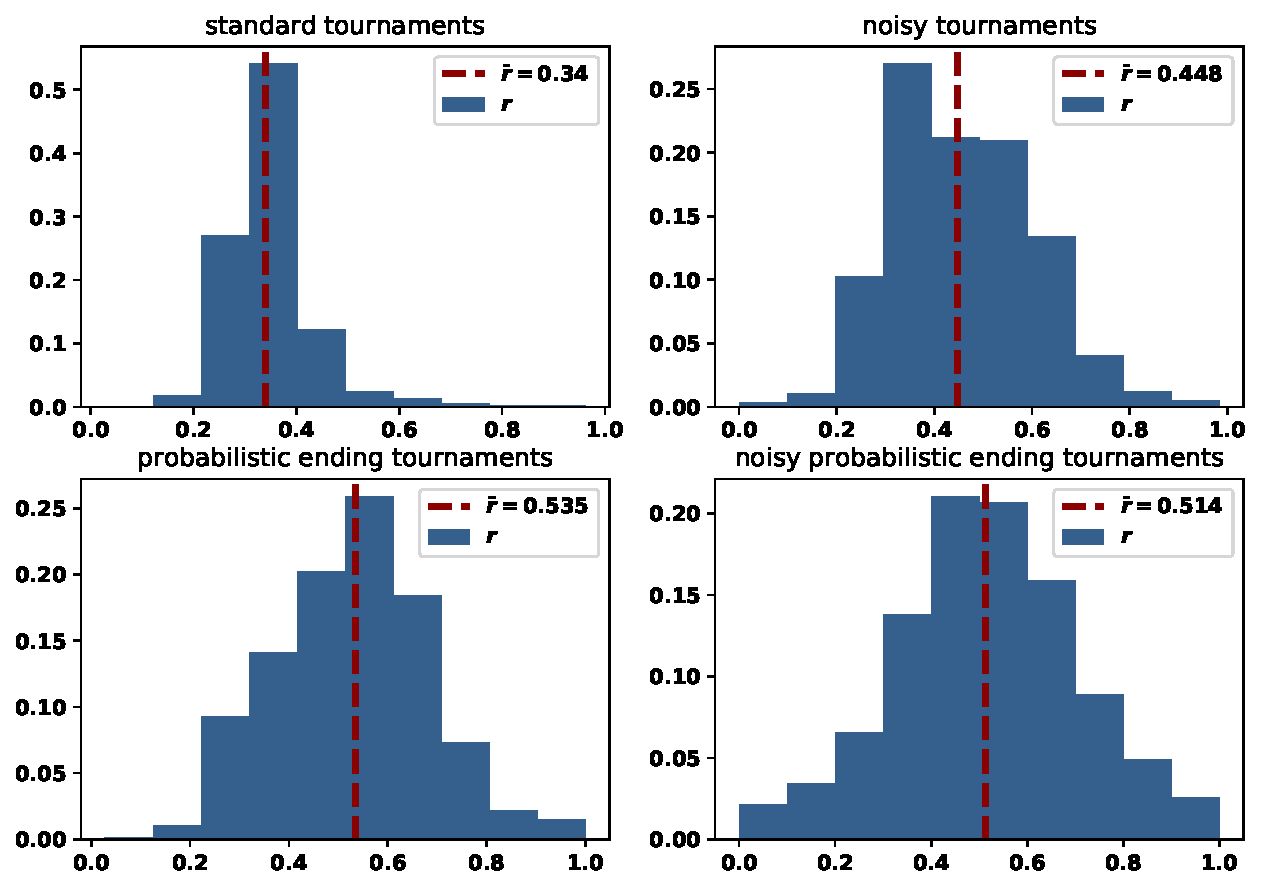
\includegraphics[width=.60\textwidth]{src/chapters/04/paper/meta-analysis-of-prisoners-dilemma-tournaments/images/tit_for_tat_r_distributions.pdf}
    \caption{\TitForTat's $r$ distribution in tournaments. Lower values of \(r\)
    correspond to better performances. The best performance
    of the strategy has been in standard tournaments where it achieved a $\bar{r}$
    of 0.34.}
    \label{fig:tit_for_tat_r_distribution}
\end{figure}

The top 15 strategies for each tournament type based on \(\bar{r}\) are given in
Table~\ref{table:top_performances}. The data collection process was designed such
that the probabilities of noise and ending of the match varied between 0 and
1. However, commonly used values for these probabilities are values less than 0.1.
Thus,
Table~\ref{table:top_performances} also includes the top 15 strategies in noisy
tournaments with \(p_n < 0.1\) and probabilistic ending tournaments with \(p_e <
0.1\). The \(r\) distributions for the top ranked strategies of Table~\ref{table:top_performances}
are given by Figure~\ref{fig:r_distributions}.

\newcolumntype{g}{>{\columncolor{Gray}}l}
\begin{table}[!htbp]
    \begin{center}
    \resizebox{\textwidth}{!}{
        \begin{tabular}{lggllggllr}
\toprule
& \multicolumn{2}{g}{Standard} & \multicolumn{2}{c}{Noisy} & \multicolumn{2}{g}{Probabilistic ending} &  \multicolumn{2}{c}{Noisy probabilistic ending} \\
\midrule
& Name & $\bar{r}$ &                 Name & $\bar{r}$ &               Name & $\bar{r}$ &                 Name & $\bar{r}$ \\
\midrule
0  &            Evolved HMM 5 &   0.00667 &                 Grumpy &   0.14020 &          Fortress4 &   0.01266 &           Alternator &   0.30370 \\
1  &           Evolved FSM 16 &   0.00995 &                    $e$ &   0.19388 &           Defector &   0.01429 &               $\phi$ &   0.30978 \\
2  &     EvolvedLookerUp2 2 2 &   0.01064 &         Tit For 2 Tats &   0.20617 &  Better and Better &   0.01587 &                  $e$ &   0.31250 \\
3  &  Evolved FSM 16 Noise 05 &   0.01667 &  Slow Tit For Two Tats &   0.20962 &    Tricky Defector &   0.01875 &                $\pi$ &   0.31686 \\
4  &        PSO Gambler 2 2 2 &   0.02143 &           Cycle Hunter &   0.21538 &          Fortress3 &   0.02174 &    Limited Retaliate &   0.35263 \\
5  &              Evolved ANN &   0.02878 &         Risky QLearner &   0.22222 &     Gradual Killer &   0.02532 &     Anti Tit For Tat &   0.35431 \\
6  &            Evolved ANN 5 &   0.03390 &            Retaliate 3 &   0.22887 &         Aggravater &   0.02778 &          Retaliate 3 &   0.35563 \\
7  &        PSO Gambler 1 1 1 &   0.03704 &          Cycler CCCCCD &   0.23507 &             Raider &   0.03077 &  Limited Retaliate 3 &   0.35563 \\
8  &            Evolved FSM 4 &   0.04891 &            Retaliate 2 &   0.23913 &         Cycler DDC &   0.04545 &            Retaliate &   0.35714 \\
9  &         PSO Gambler Mem1 &   0.05036 &        Defector Hunter &   0.24038 &        Hard Prober &   0.05128 &          Retaliate 2 &   0.35767 \\
10 &                 Winner12 &   0.06011 &              Retaliate &   0.24177 &         SolutionB1 &   0.06024 &  Limited Retaliate 2 &   0.36134 \\
11 &             Fool Me Once &   0.06140 &    Hard Tit For 2 Tats &   0.25000 &      Meta Minority &   0.06077 &             Hopeless &   0.36842 \\
12 &                      DBS &   0.07143 &               ShortMem &   0.25286 &              Bully &   0.06081 &    Arrogant QLearner &   0.40651 \\
13 &            DoubleCrosser &   0.07200 &    Limited Retaliate 3 &   0.25316 &    Fool Me Forever &   0.07080 &    Cautious QLearner &   0.40909 \\
14 &              BackStabber &   0.07519 &      Limited Retaliate &   0.25706 &             EasyGo &   0.07101 &      Fool Me Forever &   0.41764 \\
\bottomrule
    \end{tabular}
    
    }
\end{center}
\caption{Top performances for each tournament type based on $\bar{r}$. The
results of each type are based on 11420 unique tournaments. The
results for noisy tournaments with \(p_n < 0.1\) are based on 1151 tournaments,
and for probabilistic ending tournaments with \(p_e < 0.1\) on 1139. The top
ranks indicate that trained strategies perform well in a variety of
environments, but so do simple deterministic strategies. The normalised medians
are close to 0 for most environments, except environments with noise not
restricted to 0.1 regardless of the number of turns. Noisy and noisy probabilistic
ending tournaments have the highest medians.}
\label{table:top_performances}
\end{table}

\begin{figure*}[!htbp]
    \centering
    \begin{subfigure}{0.47\textwidth}
        \centering
        \includegraphics[width=\textwidth]{src/chapters/04/paper/meta-analysis-of-prisoners-dilemma-tournaments/images/r_distribution_standard.pdf}
        \caption{$r$ distributions of top 15 strategies in standard tournaments.}\label{fig:std_results}
    \end{subfigure}
    \hfill
    \begin{subfigure}{0.47\textwidth}
        \centering
        \includegraphics[width=\textwidth]{src/chapters/04/paper/meta-analysis-of-prisoners-dilemma-tournaments/images/r_distribution_noise_subset.pdf}
        \caption{$r$ distributions of top 15 strategies in noisy tournaments with \(p_n < 0.1\).}\label{fig:noise_subset_results}
    \end{subfigure}
    \vskip\baselineskip
    \begin{subfigure}{0.47\textwidth}
        \centering
        \includegraphics[width=\textwidth]{src/chapters/04/paper/meta-analysis-of-prisoners-dilemma-tournaments/images/r_distribution_noise.pdf}
        \caption{$r$ distributions of top 15 strategies in noisy tournaments.}\label{fig:noise_results}
    \end{subfigure}
    \quad
    \begin{subfigure}{0.47\textwidth}
        \centering
        \includegraphics[width=\textwidth]{src/chapters/04/paper/meta-analysis-of-prisoners-dilemma-tournaments/images/r_distribution_probend_subset.pdf}
        \caption{\(r\) distributions of top 15 strategies in 1139 probabilistic ending
        tournaments with \(p_e < 0.1\).}
        \label{fig:probend_subset_results}
    \end{subfigure}
    \vskip\baselineskip
    \begin{subfigure}{0.47\textwidth}
        \centering
        \includegraphics[width=\textwidth]{src/chapters/04/paper/meta-analysis-of-prisoners-dilemma-tournaments/images/r_distribution_probend.pdf}
        \caption{$r$ distributions of top 15 strategies in probabilistic ending tournaments.}\label{fig:probend_results}
    \end{subfigure}
    \quad
    \begin{subfigure}{0.47\textwidth}
        \centering
        \includegraphics[width=\textwidth]{src/chapters/04/paper/meta-analysis-of-prisoners-dilemma-tournaments/images/r_distribution_probend_noise.pdf}
        \caption{$r$ distributions of top 15 strategies in noisy probabilistic ending tournaments.}
        \label{fig:probend_noise_results}
    \end{subfigure}
    \caption{\(r\) distributions of the top 15 strategies in different
    environments. A lower value of \(\bar{r}\) corresponds to a more successful
    performance. A strategy's \(r\) distribution skewed towards zero indicates
    that the strategy ranked highly in most tournaments it participated in. Most
    distributions are skewed towards zero except the distributions with
    unrestricted noise, supporting the conclusions from
    Table~\ref{table:top_performances}.}\label{fig:r_distributions}
\end{figure*}

In standard tournaments 10 out of the 15 top strategies were introduced
in~\cite{Harper2017}. These are strategies based on finite state automata (FSM),
hidden Markov models (HMM), artificial neural networks (ANN), lookup tables
(LookerUp) and stochastic lookup tables (Gambler) that have been trained using
reinforcement learning algorithms (evolutionary and particle swarm algorithms).
They have been trained to perform well against a subset of the strategies
in APL in a standard tournament, thus their performance in the
specific setting was anticipated although still noteworthy given the random
sampling of tournament participants. \DoubleCrosser, \BackStabber and \FoolMeOnce, are
strategies not from the literature but from the APL. \DoubleCrosser is an extension
of \BackStabber and both strategies make use of the number of turns because they are
set to defect on the last two rounds. It should be noted that these
strategies can be characterised as ``cheaters'' because the source code of the strategies
allows them to know the number of turns in a match (unless the match has a probabilistic ending). These strategies were expected to not perform as well in
tournaments where the number of turns is not specified. Finally, \WinnerTwelve~\cite{mathieu2017}
and \DBS~\cite{Au2006} are both from the literature.
\DBS is a strategy specifically designed for noisy environments, however, it ranks
highly in standard tournaments as well. Similarly the fourth ranked player,
\EvolvedFSMSixTeenNoiseZeroFive, was
trained for noisy tournaments yet performs well in standard tournaments.
Figure~\ref{fig:std_results} shows that these strategies typically perform
well in any standard tournament in which they participate.

In the case of noisy tournaments with smaller noise \(p_n < 0.1\) the top
performing strategies
include strategies specifically designed for noisy tournaments. These are \DBS,
\EvolvedFSMSixTeenNoiseZeroFive, \EvolvedANNFiveNoiseZeroFive, \PSOGamblerTwoTwoTwoNoiseZeroFive and
\OmegaTFT~\cite{kendall2007iterated}. \OmegaTFT, another strategy designed
to break the deadlocking cycles of \(CD\) and \(DC\) that \TitForTat can fall into in noisy
environments, places 10th. The rest of the top ranks are
occupied by strategies which performed well in standard tournaments and
deterministic strategies such as \SpitefulTitForTat~\cite{prison},
\LevelPunisher~\cite{Eckhart2015}, \EugineNier~\cite{lesswrong}.

In contrast, the performance of the top ranked strategies in noisy environments
when \(p_n\in [0, 1]\) is bimodal. The top strategies include strategies which
decide their actions based on the cooperation to defection ratio, such as
\ShortMem~\cite{Andre2013}, \Grumpy~\cite{axelrodproject} and
\e~\cite{axelrodproject}, and the \Retaliate strategies which are designed to
defect if the opponent has tricked them more often than a given percentage of the times that
they have done the same. The bimodality of the \(r\) distributions is explained
by Figure~\ref{fig:effect_of_noise} which demonstrates that the top 6 strategies
were highly ranked due to the their performance in tournaments with \(p_n>0.5\),
and that in tournaments with \(p_n<0.5\) they
performed poorly. At a noisy level of \(0.5\) or greater, mostly cooperative strategies
become mostly defectors and vice versa.

\begin{figure}[!htbp]
    \centering
    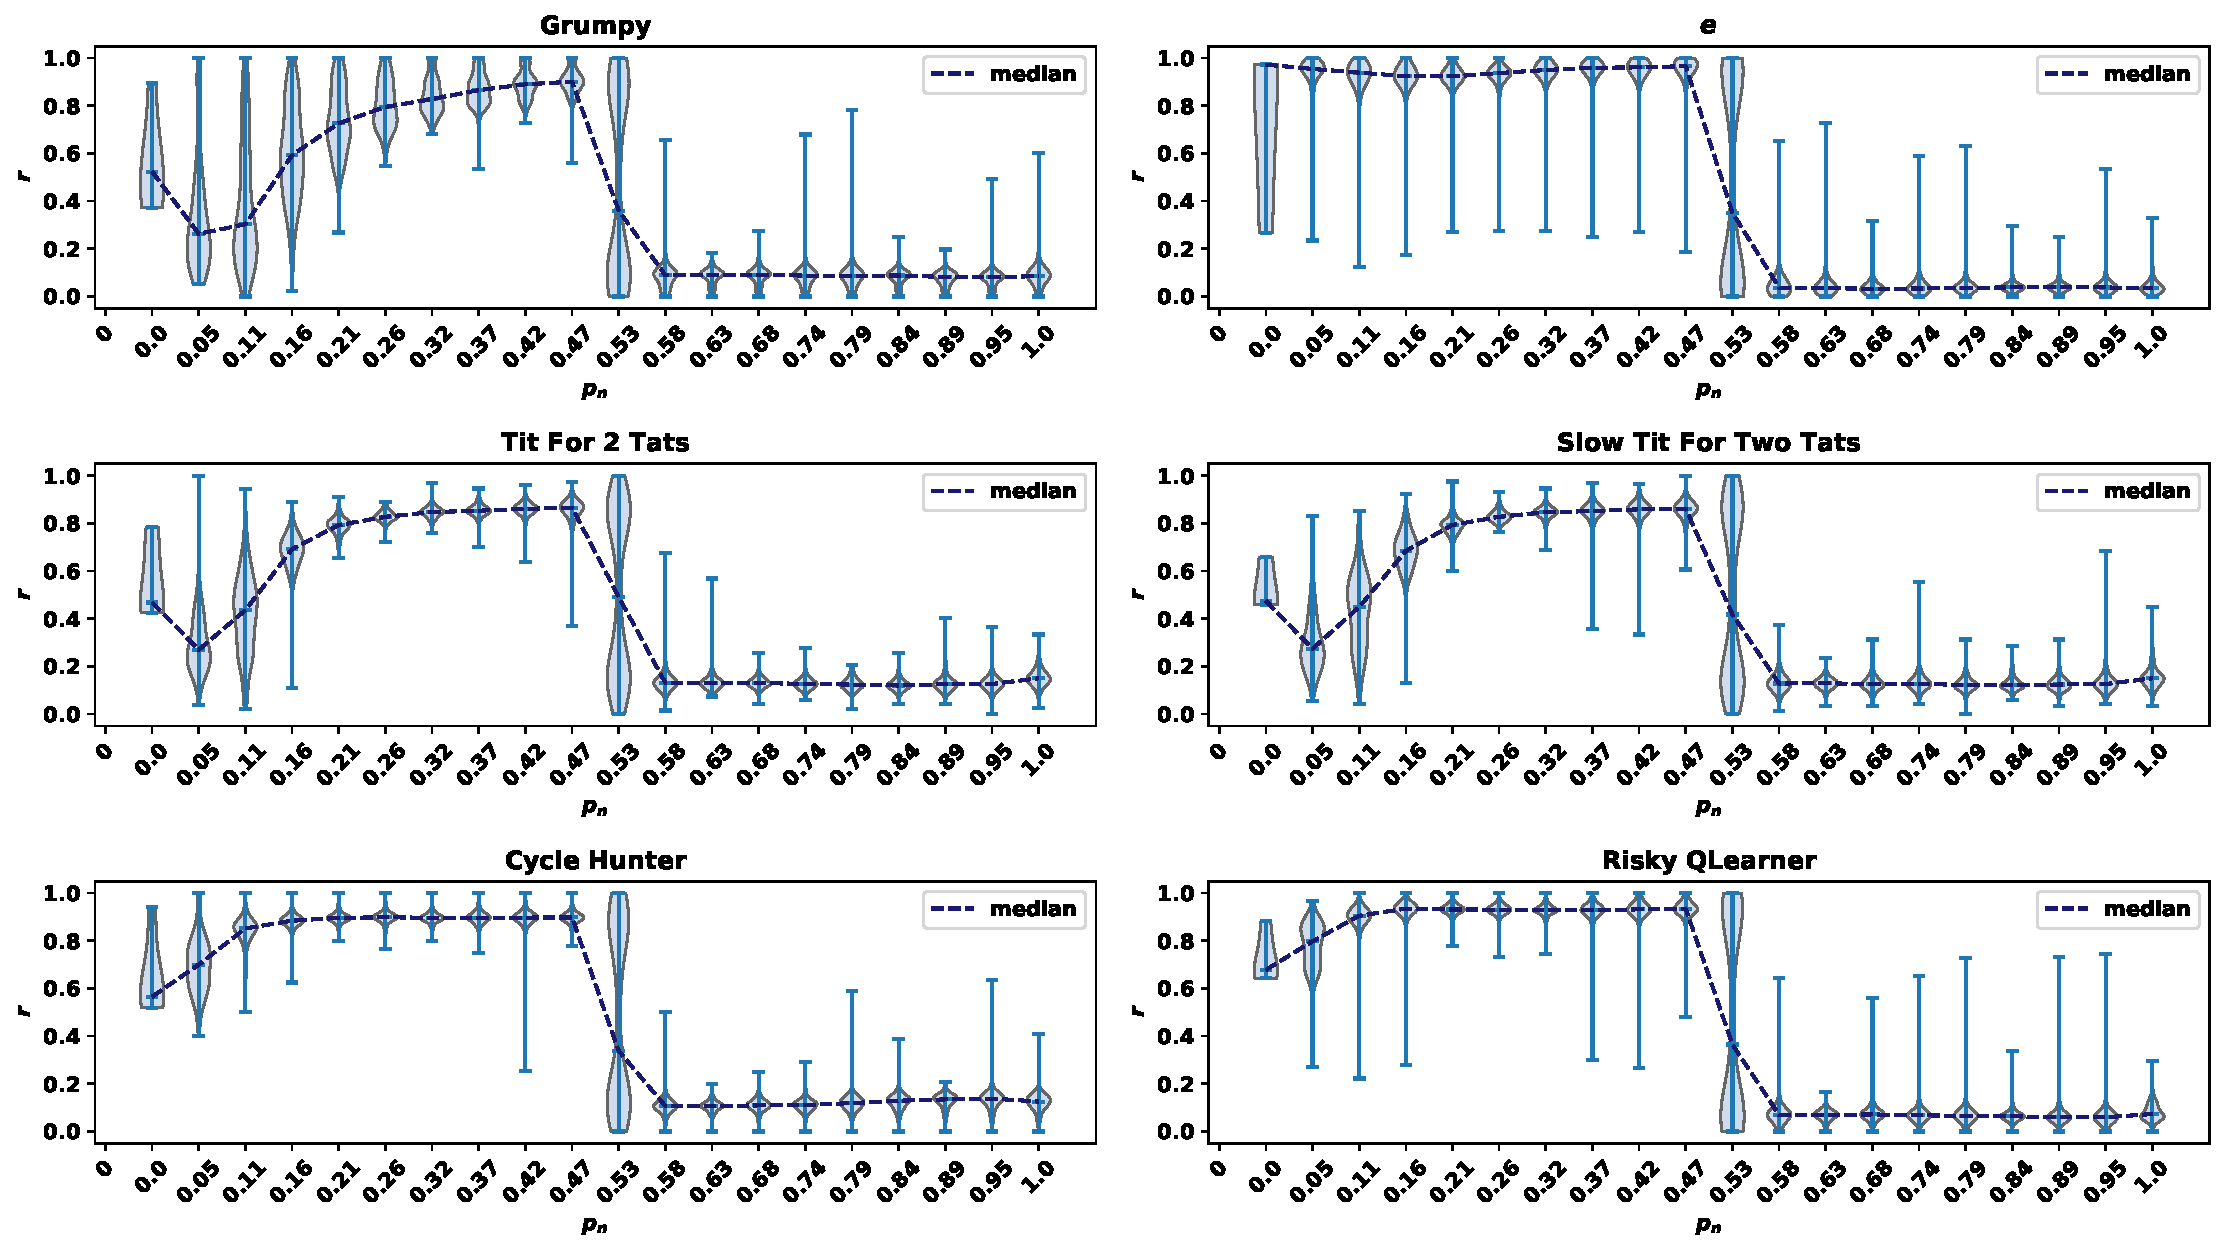
\includegraphics[width=\textwidth]{src/chapters/04/paper/meta-analysis-of-prisoners-dilemma-tournaments/images/noise_effect.pdf}
    \caption{Normalised rank \(r\) distributions for top 6 strategies in noisy tournaments over
    the probability of noisy ($p_n$).}
    \label{fig:effect_of_noise}
\end{figure}

The most effective strategies in probabilistic ending
tournaments with \(p_e< 0.1\) are a series of ensemble Meta strategies, trained strategies
which performed well
in standard tournaments, and \Grudger~\cite{axelrodproject} and \SpitefulTitForTat~\cite{prison}.
The Meta strategies~\cite{axelrodproject} utilise a team of
strategies and aggregate the potential actions of the team members into a single action
in various ways. Figure~\ref{fig:probend_subset_results} indicates that these strategies
performed well in any probabilistic ending tournament.

In probabilistic ending tournaments with \(p_e \in [0, 1]\) the top ranks are
mostly occupied by defecting strategies such as \BetterandBetter, \GradualKiller,
\HardProber (all from~\cite{axelrodproject}), \Bully (\ReverseTitForTat)~\cite{Nachbar1992}
and \Defector, and a series of strategies based on finite
state automata introduced by Daniel Ashlock and Wendy Ashlock: \FortressThree,
\FortressFour (both introduced in~\cite{Ashlock2006}), \Raider~\cite{Ashlock2014}
and \SolutionBOne~\cite{Ashlock2014}. The success of defecting strategies in
probabilistic ending tournaments is due to larger values of
\(p_e\) which lead to shorter matches (the expected number of rounds is \(1 / p_e\)), so the
impact of the PD being iterated is subdued. This is captured by the Folk
Theorem~\cite{Fudenberg2009} as defecting strategies do better when the likelihood
of the game ending in the next turn increases.
This is demonstrated by Figure~\ref{fig:effect_of_probend}, which gives the
distributions of \(r\) for the top 6 strategies in probabilistic ending tournaments
over \(p_e\).

\begin{figure}[!htbp]
    \centering
    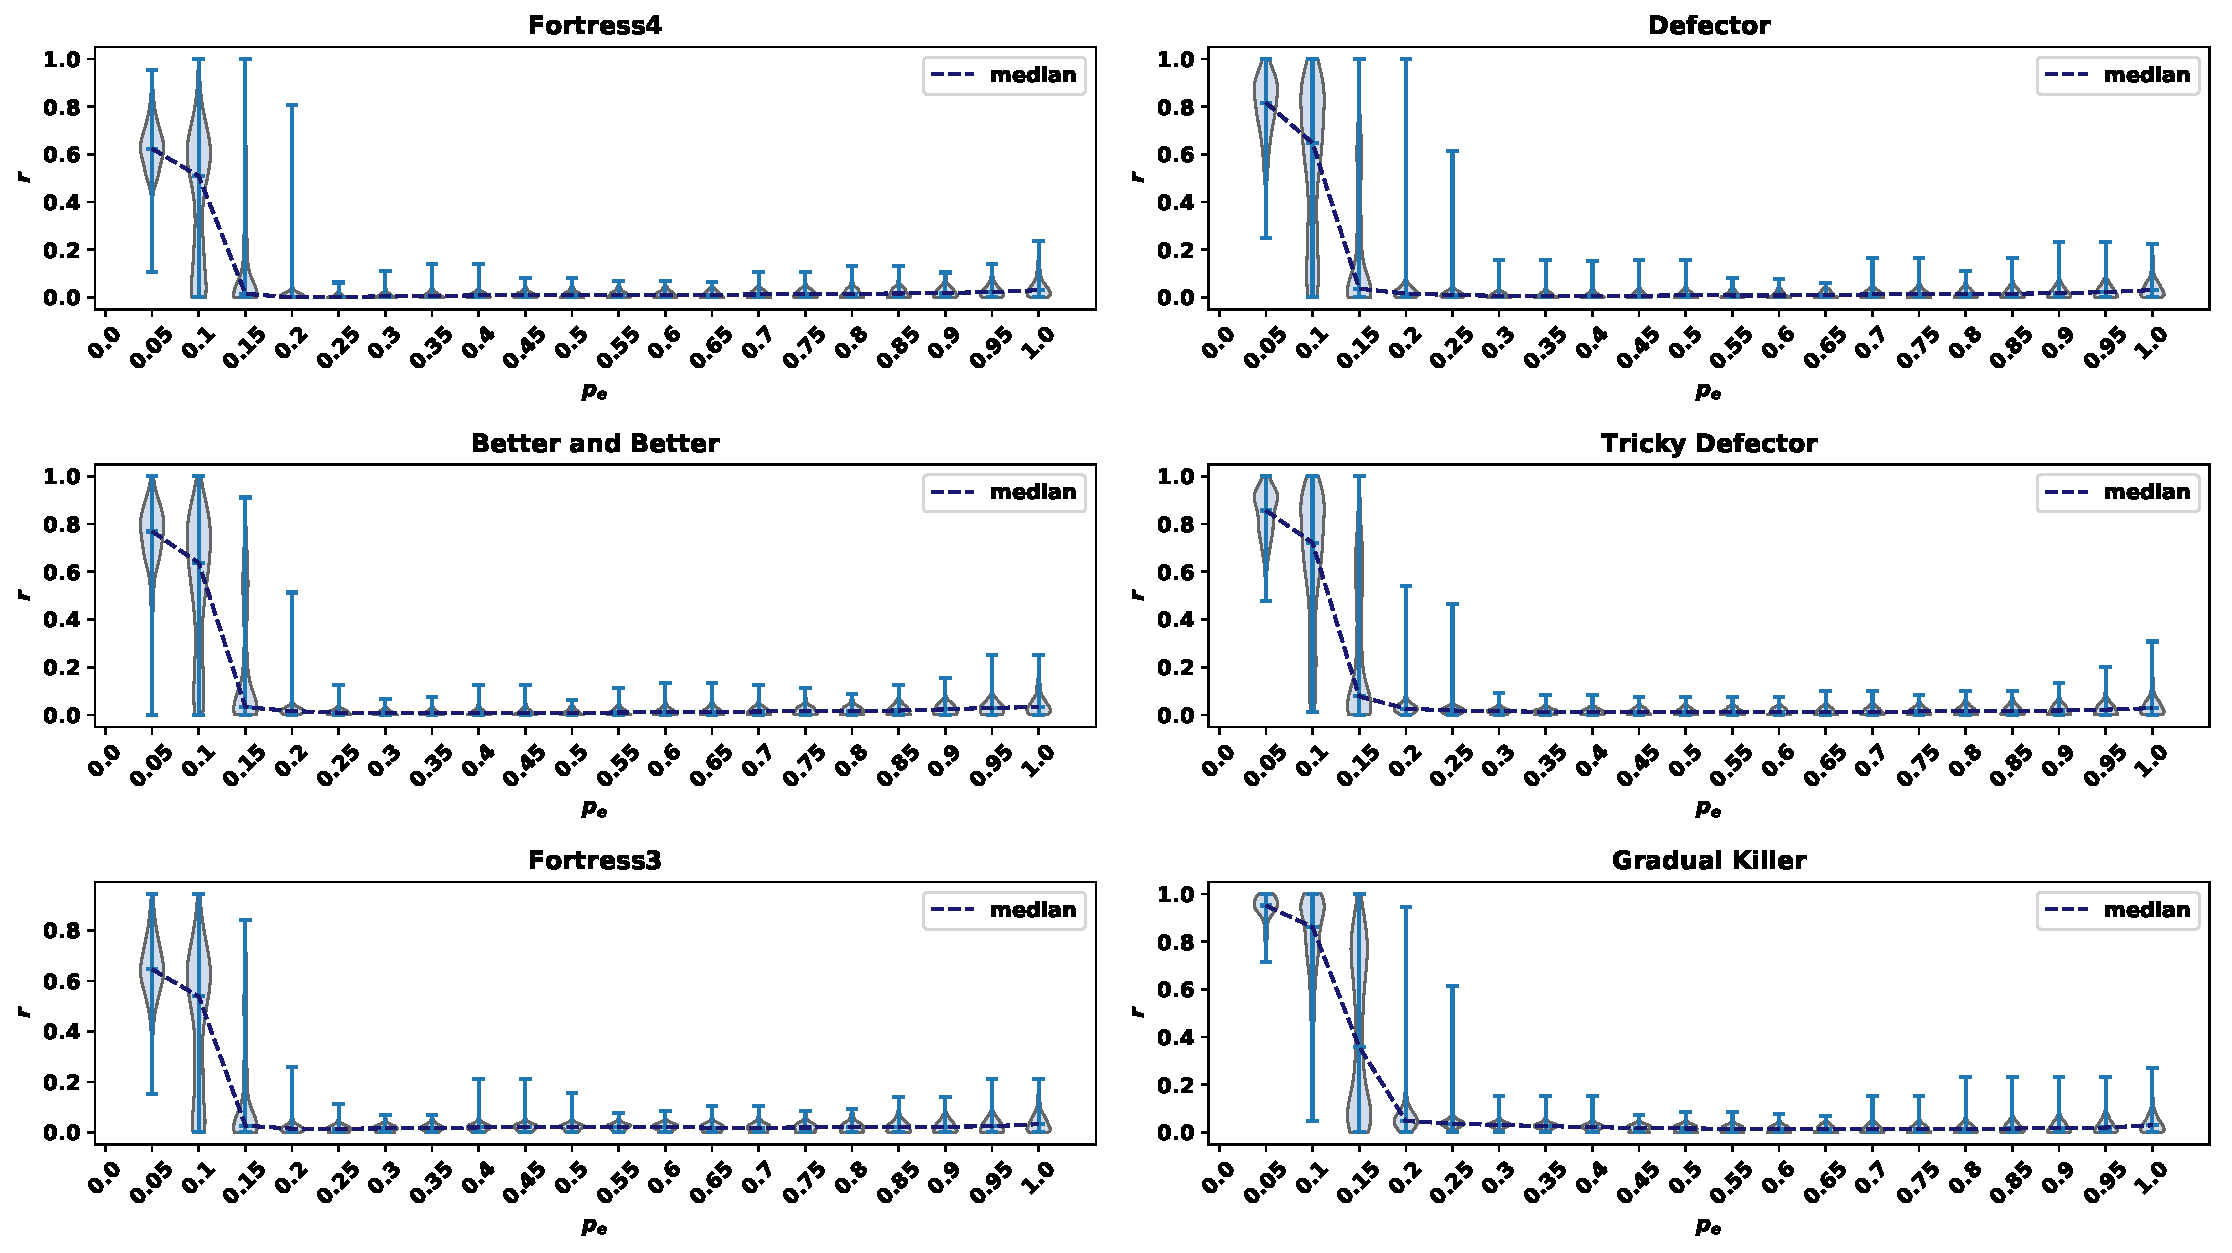
\includegraphics[width=\textwidth]{src/chapters/04/paper/meta-analysis-of-prisoners-dilemma-tournaments/images/folk_theorem.pdf}
    \caption{Normalised rank \(r\) distributions for top 6 strategies in probabilistic ending tournaments
    over $p_e$. The 6 strategies start of with a high median rank,
    however, their ranked decreased as the the probability of the game ending
    increased and at the point of \(p_e = 0.1\).}
    \label{fig:effect_of_probend}
\end{figure}

The top performances in tournaments with both noise and a probabilistic ending
and the top performances over the entire data set have the largest median values
compared to the top rank strategies of the other tournament types,
Figure~\ref{fig:probend_noise_results} and Figure~\ref{fig:overall_results}. The
\(\bar{r}\) for the top strategy is approximately at 0.3, indicating that the
most successful strategy can on average just place in the top 30\% of the
competition.

\begin{table}[!htbp]
    \centering
    \resizebox{.3\textwidth}{!}{
    \begin{tabular}{lr}
\toprule
Name                       &     \(\bar{r}\) \\
\midrule
Limited Retaliate 3        &            0.286 \\
Retaliate 3                &            0.297 \\
Retaliate 2                &            0.302 \\
Limited Retaliate 2        &            0.304 \\
Limited Retaliate          &            0.311 \\
Retaliate                  &            0.317 \\
BackStabber                &            0.324 \\
DoubleCrosser              &            0.331 \\
Nice Meta Winner           &            0.350 \\
PSO Gambler 2 2 2 Noise 05 &            0.351 \\
Grudger                    &            0.352 \\
NMWE Memory One            &            0.357 \\
Evolved HMM 5              &            0.358 \\
Nice Meta Winner Ensemble  &            0.359 \\
Forgetful Fool Me Once     &            0.359 \\
\bottomrule
\end{tabular}
}
    \caption{Top performances over all the tournaments. The top ranks include
    strategies that have been previously mentioned. The set of \Retaliate
    strategies occupy the top spots followed by \BackStabber and \DoubleCrosser.
    The distributions of the \Retaliate strategies have no statistical
    difference. PSO Gambler and \EvolvedHMMFive are trained strategies introduced
    in~\cite{Harper2017} and \NiceMetaWinner and \NMWEMemoryOne are strategies
    based on teams. \Grudger is a strategy from Axelrod's original tournament and
    Forgetful \FoolMeOnce is based on the same approach as
    \Grudger.}\label{table:overall_results}
\end{table}

\begin{figure}[!htbp]
        \centering
        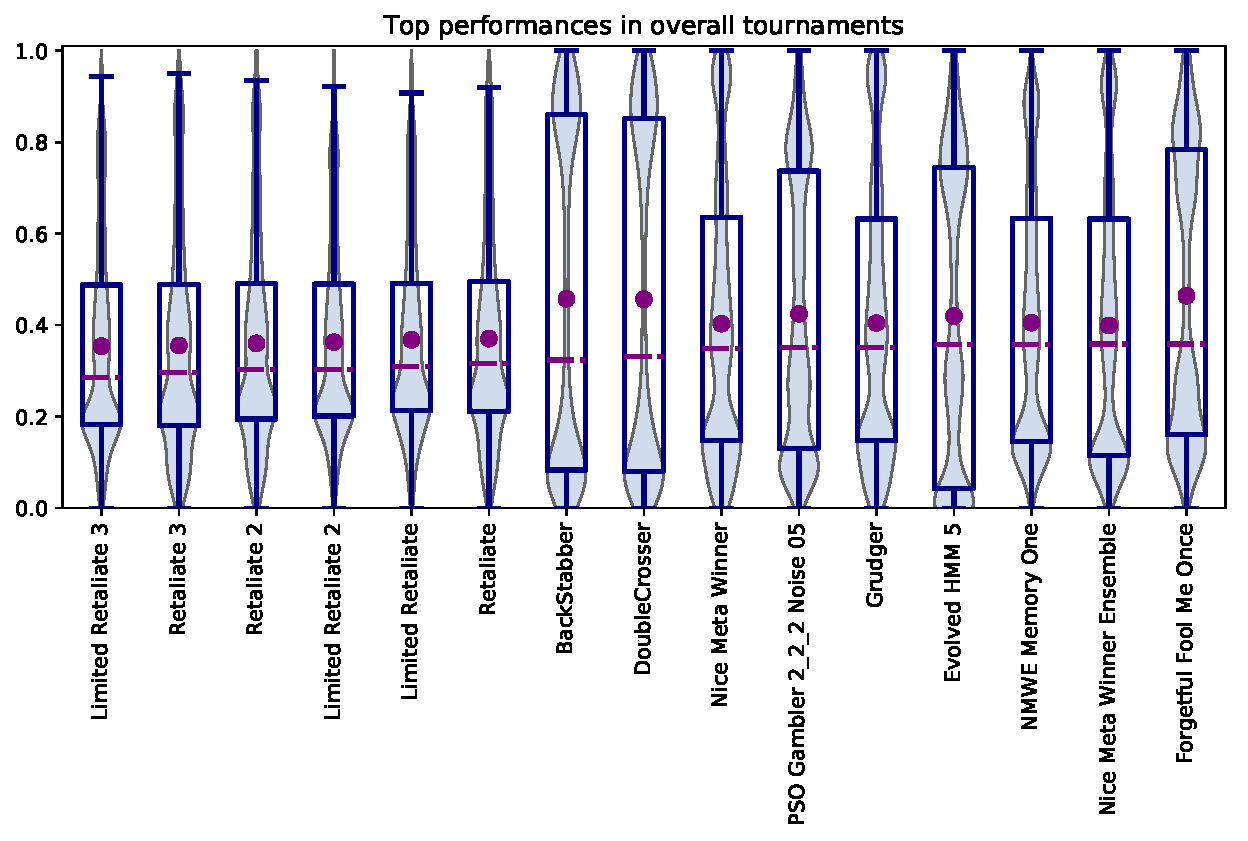
\includegraphics[width=.65\textwidth]{src/chapters/04/paper/meta-analysis-of-prisoners-dilemma-tournaments/images/performance_merged.pdf}
        \caption{\(r\) distributions for best performed strategies in the data set~\cite{Glynatsi2019_meta}.
        A lower value of \(\bar{r}\) corresponds to a more successful
        performance.}
        \label{fig:overall_results}
\end{figure}

On the whole, the analysis of this section has shown that:

\begin{itemize}
    \item In standard tournaments the dominating strategies were
    strategies that had been trained using reinforcement learning techniques.
    \item In noisy environments where the noise probability strictly less than
    0.1 was considered, the successful strategies were strategies specifically
    designed or trained for noisy environments.
    \item In probabilistic ending tournaments most of the highly ranked
    strategies were defecting strategies and trained finite state automata, all
    by the authors of~\cite{Ashlock2006, Ashlock2014}. These strategies ranked
    high due to their performance in tournaments where the probability of the
    game ending after each turn was bigger than 0.1.
    \item In probabilistic tournaments with \(p_e\) less than 0.1 the highly
    ranked strategies were strategies based on the behaviour of others.
    \item From the collection of strategies considered here,  no strategy can be
    consistently successful in noisy environments, except if the value of noise
    is constrained to less than a 0.1.
\end{itemize}

Though there is not a single strategy that repeatably outranks all others in any
of the distinct tournament types, or even across the tournament types, there
are specific types of strategies have been repeatably ranked in the top ranks.
These have been strategies that have been trained, strategies that retaliate,
and strategies that would adapt their behaviour based on preassigned rules
to achieve the highest outcome. These results contradict some of Axelrod's suggestions,
and more specifically, the suggestions `Do not be clever' and `Do not be envious'.
The features and properties contributing a strategy's success are further
explored in section~\ref{section:evaluation_of_performance}.

\section{Evaluation of performance}\label{section:evaluation_of_performance}

This section examines the performance of the strategies based on features of strategies described in
Table~\ref{table:manual_features}. These features are measures regarding a
strategy's behaviour from the tournaments the strategies competed in as well as
intrinsic properties such as whether a strategy is deterministic or stochastic.

\newcolumntype{g}{>{\columncolor{Gray}}c}
\begin{table}[!htbp]
    \begin{center}
    \resizebox{.99\textwidth}{!}{
    \begin{tabular}{gcgcgc}
    \toprule
    feature & feature explanation &  source & value type & min value & max value \\
    \midrule
stochastic  &  If a strategy is stochastic & strategy classifier from APL & boolean  & Na &  Na \\
makes use of game &  If a strategy makes used of the game information & strategy classifier from APL & boolean  & Na &  Na \\
makes use of length &  If a strategy makes used of the number of turns & strategy classifier from APL & boolean  & Na &  Na \\
memory usage &  The memory size of a strategy divided by the number of turns & memory size from APL & float & 0 &  1 \\
SSE & A measure of how far a strategy is from ZD behaviour & method described in~\cite{Knight2019} & float & 0 & 1 \\
max cooperating rate $(C_{\text{max}})$  & The biggest cooperating rate in a given tournament  & result summary  & float & 0 & 1\\
min cooperating rate $(C_{\text{min}})$ & The smallest cooperating rate in a given tournament  & result summary  & float & 0 & 1\\
median cooperating rate $(C_{\text{median}})$ & The median cooperating rate in a given tournament  & result summary  & float & 0 & 1\\
mean cooperating rate $(C_{\text{mean}})$ & The mean cooperating rate in a given tournament  & result summary  & float & 0 & 1 \\
$C_r$ / $C_{\text{max}}$ & A strategy's cooperating rate divided by the maximum & result summary  & float & 0 & 1 \\
$C_{\text{min}}$ / $C_r$ & A strategy's cooperating rate divided by the minimum & result summary  & float & 0 & 1 \\
$C_r$ / $C_{\text{median}}$ & A strategy's cooperating rate divided by the median  & result summary  & float & 0 & 1\\
$C_r$ / $C_{\text{mean}}$ & A strategy's cooperating rate divided by the mean & result summary  & float & 0 & 1 \\
$C_r$ & The cooperating ratio of a strategy & result summary  & float & 0 & 1 \\
$CC$ to $C$ rate & The probability a strategy will cooperate after a mutual cooperation & result summary  & float & 0 & 1\\
$CD$ to $C$ rate & The probability a strategy will cooperate after being betrayed by the opponent & result summary  & float & 0 & 1 \\
$DC$ to $C$ rate & The probability a strategy will cooperate after betraying the opponent & result summary  & float & 0 & 1 \\
$DD$ to $C$ rate & The probability a strategy will cooperate after a mutual defection & result summary  & float & 0 & 1 \\
$p_n$ & The probability of a player's action being flip at each interaction & trial summary & float & 0 & 1 \\
$n$ & The number of turns & trial summary & integer & 1 & 200 \\
$p_e$ & The probability of a match ending in the next turn & trial summary & float & 0 & 1 \\
$N$ & The number of strategies in the tournament & trial summary & integer & 3 & 195 \\
$k$ & The number of repetitions of a given tournament & trial summary & integer & 10 & 100 \\
    \bottomrule
        \end{tabular}}
    \end{center}
    \caption{The features which are included in the performance evaluation
    analysis. Stochastic, makes use of length and makes use of game are APL
    classifiers that determine whether a strategy is stochastic or deterministic,
    whether it makes use of the number of turns or the game's payoffs. The
    memory usage is calculated as the number of turns the strategy considers to
    make an action (which is specified in the APL) divided by the number of
    turns. The SSE (introduced in~\cite{Knight2019}) shows how close a strategy
    is to behaving as a ZDs, and subsequently, in an extortionate way. The
    method identifies the ZDs closest to a given strategy and calculates the
    algebraic distance between them, defined as SSE. More details on the measure
    are presented in Chapter~\ref{chapter:memory_one}. A SSE value of 1 indicates
    no extortionate behaviour at all whereas a value of 0 indicates that a
    strategy is behaving as a ZDs. The rest of the features considered are the $CC$
    to $C$, $CD$ to $C$, $DC$ to $C$, and $DD$ to $C$ rates as well as
    cooperating ratio of a strategy, the minimum (\(C_{min}\)), maximum
    (\(C_{max}\)), mean (\(C_{mean}\)) and median (\(C_{median}\)) cooperating
    ratios of each tournament.}
    \label{table:manual_features}
\end{table}

The memory usage of strategies is the number of
rounds of play used by the strategy divided by the number of turns in each match.
For example, \WinnerTwelve uses the previous two rounds of play, and if participating
in a match with 100 turns its memory usage would be 2/100.
For strategies with an infinite memory size, for example \EvolvedFSMSixTeenNoiseZeroFive,
memory usage is equal to 1.
Note that for tournaments with a probabilistic
ending the number of turns was not collected, so the memory usage feature is not
used for probabilistic ending tournaments.

The correlation coefficients between the features of
Table~\ref{table:manual_features} the median score and the median normalised
rank are given by Table~\ref{table:correlations}. The correlation coefficients
between all features of Table~\ref{table:manual_features} have been calculated
and a graphical representation can be found in the
Appendix~\ref{app:correlations}.

\newcolumntype{g}{>{\columncolor{Gray}}c}
\begin{table}[!htbp]
    \begin{center}
    \resizebox{.9\textwidth}{!}{
        \begin{tabular}{lggccggccggg}
    \toprule
    &  \multicolumn{2}{g}{Standard} & \multicolumn{2}{c}{Noisy} & \multicolumn{2}{g}{Probabilistic ending} &  \multicolumn{2}{c}{Noisy probabilistic ending} &  \multicolumn{2}{g}{Overall} \\
\midrule
{} &  $r$ &  median score &  $r$ &  median score &  $r$ &  median score &  $r$ &  median score &  $r$ &  median score\\
\midrule
$CC$ to $C$ rate     & -0.501 &  0.501 &   0.414 &  -0.504 &   0.408 &  -0.323 &   0.260 &   0.022 &  -0.501 &  0.501 \\
$CD$ to $C$ rate     &  0.226 & -0.199 &   0.456 &  -0.330 &   0.320 &  -0.017 &   0.205 &  -0.220 &   0.226 & -0.199 \\
$C_r$                & -0.323 &  0.384 &   0.711 &  -0.678 &   0.714 &  -0.832 &   0.579 &  -0.135 &  -0.323 &  0.384 \\
$C_r$ / $C_{max}$    & -0.323 &  0.381 &   0.616 &  -0.551 &   0.714 &  -0.833 &   0.536 &  -0.116 &  -0.323 &  0.381 \\
$C_r$ / $C_{mean}$   & -0.331 &  0.358 &   0.731 &  -0.740 &   0.721 &  -0.861 &   0.649 &  -0.621 &  -0.331 &  0.358 \\
$C_r$ / $C_{median}$ & -0.331 &  0.353 &   0.652 &  -0.669 &   0.712 &  -0.852 &   0.330 &  -0.466 &  -0.331 &  0.353 \\
$C_r$ / $C_{min}$    &  0.109 & -0.080 &  -0.358 &   0.250 &  -0.134 &   0.150 &  -0.368 &   0.113 &   0.109 & -0.080 \\
$C_{max}$            & -0.000 &  0.049 &   0.000 &   0.023 &  -0.000 &   0.046 &   0.000 &  -0.004 &  -0.000 &  0.049 \\
$C_{mean}$           & -0.000 &  0.229 &  -0.000 &   0.271 &   0.000 &   0.200 &   0.000 &   0.690 &  -0.000 &  0.229 \\
$C_{median}$         &  0.000 &  0.209 &  -0.000 &   0.240 &  -0.000 &   0.187 &  -0.000 &   0.673 &   0.000 &  0.209 \\
$C_{min}$            &  0.000 &  0.084 &   0.000 &  -0.017 &  -0.000 &   0.007 &  -0.000 &   0.041 &   0.000 &  0.084 \\
$DC$ to $C$ rate     &  0.127 & -0.100 &   0.509 &  -0.504 &  -0.018 &   0.033 &   0.341 &  -0.016 &   0.127 & -0.100 \\
$DD$ to $C$ rate     &  0.412 & -0.396 &   0.533 &  -0.436 &  -0.103 &   0.176 &   0.378 &  -0.263 &   0.412 & -0.396 \\
$N$                  &  0.000 & -0.009 &  -0.000 &   0.002 &  -0.000 &   0.003 &  -0.000 &   0.001 &   0.000 & -0.009 \\
$k$                  &  0.000 & -0.002 &  -0.000 &   0.003 &  -0.000 &   0.001 &  -0.000 &  -0.008 &   0.000 & -0.002 \\
$n$                  &  0.000 & -0.125 &  -0.000 &  -0.024 &       - &       - &       - &       - &   0.000 & -0.125 \\
$p_e$                &      - &      - &        - &     - &    0.000 &   0.165 &   0.000 &  -0.058 &  -0.001 &  0.001 \\
$p_n$                &      - &      - &  -0.000 &   0.207 &       - &       - &  -0.000 &  -0.650 &   0.002 & -0.000 \\
Make use of game     & -0.003 & -0.022 &   0.025 &  -0.082 &  -0.053 &  -0.108 &   0.013 &  -0.016 &  -0.003 & -0.022 \\
Make use of length   & -0.158 &  0.124 &   0.005 &  -0.123 &  -0.025 &  -0.090 &   0.014 &  -0.016 &  -0.154 &  0.117 \\
SSE                  &  0.473 & -0.452 &   0.463 &  -0.337 &  -0.156 &   0.223 &   0.305 &  -0.259 &   0.473 & -0.452 \\
memory usage         & -0.082 &  0.095 &  -0.007 &  -0.017 &       - &     - &     - &           - &  -0.084 &  0.095 \\
stochastic           &  0.006 & -0.024 &   0.022 &  -0.026 &   0.002 &  -0.130 &   0.021 &  -0.013 &   0.006 & -0.024 \\
\bottomrule
\end{tabular}

    }
\end{center}
\caption{Correlations between the features of Table~\ref{table:manual_features}
and the normalised rank and the median score.}\label{table:correlations}
\end{table}

In standard tournaments the features $CC$ to $C$, $C_r$, $C_r / C_{\text{max}}$
and the cooperating ratio compared to $C_{\text{median}}$ and $C_{\text{mean}}$
have a moderately negative effect on the normalised rank (smaller rank is better), and a moderate positive
on the median score. The SSE error and the $DD$ to $C$ rate have the opposite
effects. Thus, in standard tournaments behaving cooperatively corresponds to a
more successful performance. Even though being nice generally pays off
that does not hold against defective strategies. Being more cooperative after a mutual
defection, that is not retaliating, is associated to lesser overall success in terms of normalised rank.
Figure~\ref{fig:rates_of_winners_in_standard_tournaments} confirms that the
winners of standard tournaments always cooperate after a mutual cooperation and
almost always defect after a mutual defection.

\begin{figure}[!htbp]
    \centering
    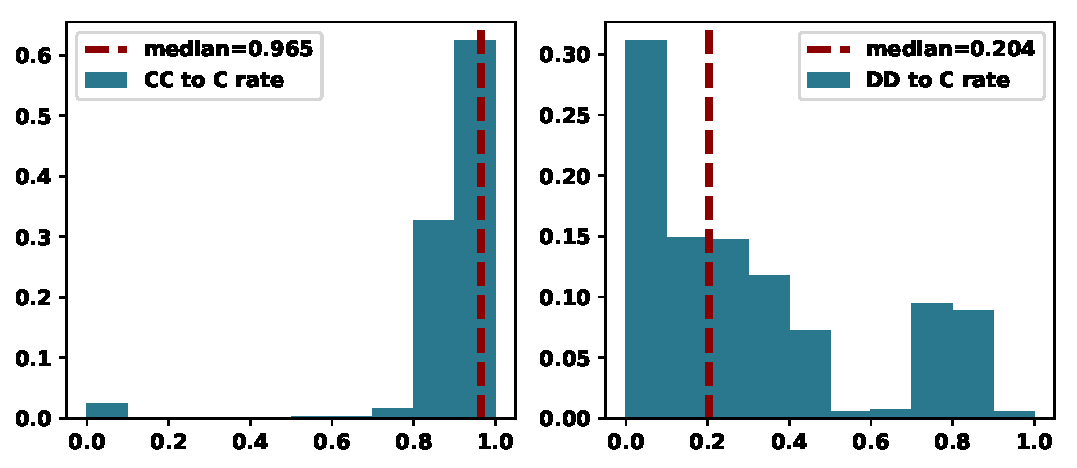
\includegraphics[width=.8\textwidth]{src/chapters/04/paper/meta-analysis-of-prisoners-dilemma-tournaments/images/rates_of_winners_in_standard_tournaments.pdf}
    \caption{Distributions of $CC$ to $C$ and $DD$ to $C$ for the winners in
    standard tournaments.}\label{fig:rates_of_winners_in_standard_tournaments}
\end{figure}

Compared to standard tournaments, in both noisy and in probabilistic ending
tournaments the higher the rates of cooperation the lower a strategy's success
and median score. A strategy would want to cooperate less than both
the mean and median cooperator in such settings. In probabilistic ending
tournaments the correlation coefficients have larger values, indicating a
stronger effect. Thus a strategy will be punished more by its cooperative
behaviour in probabilistic ending environments, supporting the results of
section~\ref{section:evaluation_of_performance}
as well. The distributions of the $C_r$ of the winners in
both tournaments are given by Figure~\ref{fig:c_r_distributions}. It confirms
that the winners in noisy tournaments cooperated less than 35\% of the time
and in probabilistic ending tournaments less than 10\%.
In noisy probabilistic ending tournaments and over all the tournaments' results,
the only features that had a moderate effect are $C_r/C_{\text{mean}},
C_r/C_{\text{max}}$ and $C_r$. In such environments cooperative behaviour
appears to be punished less than in noisy and probabilistic ending
tournaments.

\begin{figure}[!htbp]
    \centering
    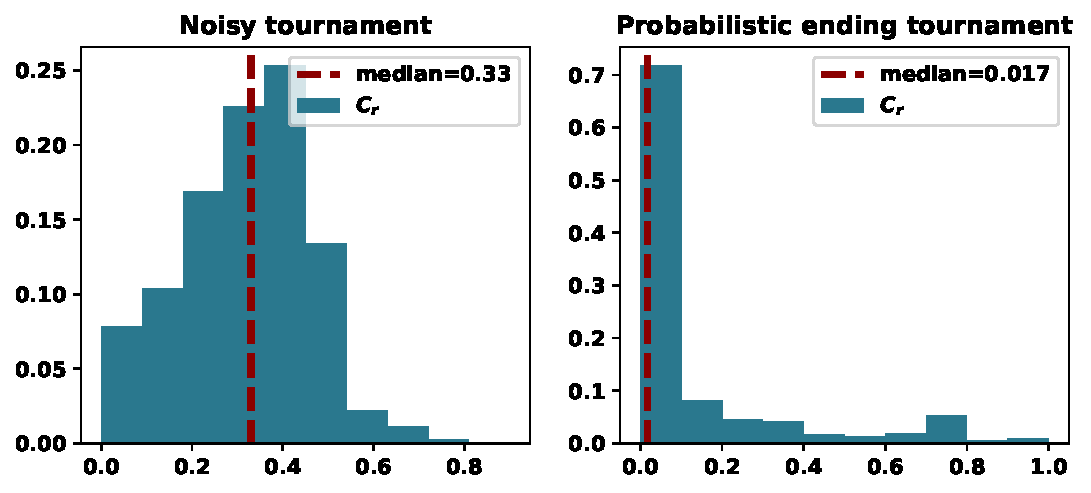
\includegraphics[width=.8\textwidth]{src/chapters/04/paper/meta-analysis-of-prisoners-dilemma-tournaments/images/c_r_winners_tournaments.pdf}
    \caption{$C_r$ distributions of the winners in noisy and in probabilistic
    ending tournaments.}\label{fig:c_r_distributions}
\end{figure}

A multivariate linear regression has been fitted to model the relationship between
the features and the normalised rank. Based on the graphical representation of
the correlation matrices given in Appendix~\ref{app:correlations} several of the
features are highly correlated and have been removed
before fitting the linear regression model. The features included are given
by Table~\ref{table:linear_regression} alongside their corresponding \(p\) values
in the distinct tournaments and their regression coefficients.

\newcolumntype{g}{>{\columncolor{Gray}}c}
\begin{table}[h]
    \begin{center}
\resizebox{\textwidth}{!}{
    \input{src/chapters/04/paper/meta-analysis-of-prisoners-dilemma-tournaments/paper/regression_table.tex}}
    \end{center}
    \caption{Results of multivariate linear regressions with \(r\) as the dependent variable.
    \(R\) squared is reported for each model.}
    \label{table:linear_regression}
\end{table}

A multivariate linear regression has also be fitted on the median score. The
coefficients and \(p\) values of the features can be found in
Appendix~\ref{app:further_regression}. The results of the two methods
are in agreement.

The feature \(C_{r} / C_{\text{mean}}\) has a statistically significant effect
across all models and a high regression coefficient. It has both a positive and
negative impact on the normalised rank depending on the environment. For
standard tournaments, Figure~\ref{fig:discussion_standard} gives the
distributions of several features for the winners of standard tournaments. The
\(C_{r} / C_{\text{mean}}\) distribution of the winner is also given in
Figure~\ref{fig:discussion_standard}. A value of \(C_r / C_{\text{mean}} = 1\)
implies that the cooperating ratio of the winner was the same as the mean
cooperating ratio of the tournament, and in standard tournaments, the median is
1. Therefore, an effective strategy in standard tournaments was the mean
cooperator of its respective tournament.

The distributions of SSE and \(CD\) to \(C\) rate for the winners of standard
tournaments are also given in Figure~\ref{fig:discussion_standard}. The SSE
distributions for the winners indicate that the strategy behaved in a ZD way in
several tournaments, however, not constantly. The winners participated in
matches where they did not try to extortionate their opponents. Furthermore, the
\(CD\) to \(C\) distribution indicates that if a strategy were to defect against
the winners the winners would reciprocate on average with a probability of 0.5.

\begin{figure}[!htbp]
    \centering
        \centering
        \includegraphics[width=\textwidth]{src/chapters/04/paper/meta-analysis-of-prisoners-dilemma-tournaments/images/standard_discussion.pdf}
        \caption{Distributions of \(C_r / C_{\text{mean}}\), SSE and \(CD\) to \(C\) ratio
        for the winners of standard tournaments. A
        value of \(C_r / C_{\text{mean}} = 1\) imply that the cooperating ratio of the
        winner was the same as the mean cooperating ratio of the tournament. An SSE distribution
        skewed towards 0 indicates a extortionate behaviour by the strategy.}
        \label{fig:discussion_standard}
\end{figure}

Similarly for the rest of the different tournaments types, and the entire data
set the distributions of \(C_r / C_{\text{mean}}\), SSE and \(CD\) to \(C\) ratio
are given by Figures~\ref{fig:discussion_noisy},~\ref{fig:discussion_probend},
\ref{fig:discussion_probend_noisy} and~\ref{fig:discussion_entire_data}.

Based on the \(C_r / C_{\text{mean}}\) distributions the successful strategies
have adapted differently to the mean cooperator depending on the tournament
type. In noisy tournaments where the median of the distribution is at 0.67, and
thereupon the winners cooperated 67\% of the time the mean cooperator did. In
tournaments with noise and a probabilistic ending the winners cooperated 60\%,
whereas in settings that the type of the tournament can vary between all the
types the winners cooperated 67\% of the time the mean cooperator did. Lastly,
in probabilistic ending tournaments above more defecting
strategies prevail (section~\ref{section:top_performances}), and this result is
reflected here.

\begin{figure}[!htbp]
    \centering
        \centering
        \includegraphics[width=\textwidth]{src/chapters/04/paper/meta-analysis-of-prisoners-dilemma-tournaments/images/noisy_discussion.pdf}
        \caption{Distributions of \(C_r / C_{\text{mean}}\), SSE and \(CD\) to \(C\) ratio
        for the winners of noisy tournaments.}
        \label{fig:discussion_noisy}
\end{figure}

The probability of noise has been observed to substantially affect optimal
behaviour.
Figure~\ref{fig:compared_to_mean_over_noise_probability} gives the ratio \(C_r /
C_{\text{mean}}\) for the winners in tournaments with noise, over the
probability of noise. From Figure~\ref{fig:noisy_discussion_over_noise} it is
clear that the cooperating only 67\% of the time the mean cooperator did is
optimal only when \(p_n \in [0.2, 0.4)\) and \(p_n \in [0.6, 0.7]\). In
environments with \(p_n < 0.1\) the winners want to be close to the mean
cooperator, similarly to standard tournaments, and as the probability of noise
is exceeding 0.5 (where the game is effectively inverted) strategies should
aim to be less and less cooperative.

Figure~\ref{fig:compared_to_mean_over_noise_probability} gives \(C_r /
C_{\text{mean}}\) for the winners over \(p_n\) in tournaments with noise and a
probabilistic ending. The optimal proportions of cooperations are different
now that the number of turns is not fixed, successful strategies
want to be more defecting that the mean cooperator, that only changes when
\(p_n\) approaches 0.5. Figure~\ref{fig:compared_to_mean_over_noise_probability}
demonstrates how the adjustments to \(C_r /C_{\text{mean}}\) change over the
noise in the to the environment, and thus supports how important adapting to
the environment is for a strategy to be successful.

\begin{figure}[!htbp]
    \centering
    \begin{subfigure}{0.485\textwidth}
        \centering
        \includegraphics[width=\textwidth]{src/chapters/04/paper/meta-analysis-of-prisoners-dilemma-tournaments/images/noisy_discussion_over_noise.pdf}
        \caption{\(C_r / C_{\text{mean}}\) distribution for winners in noisy tournaments over
        \(p_n\).}\label{fig:noisy_discussion_over_noise}
    \end{subfigure}
    \hfill
    \begin{subfigure}{0.485\textwidth}
        \centering
        \includegraphics[width=\textwidth]{src/chapters/04/paper/meta-analysis-of-prisoners-dilemma-tournaments/images/noisy_probend_discussion_over_noise.pdf}
        \caption{\(C_r / C_{\text{mean}}\) distribution for winners in noisy probabilistic ending tournaments over
        \(p_n\).}\label{fig:noisy_probend_discussion_over_noise}
    \end{subfigure}
    \caption{\(C_r / C_{\text{mean}}\) distributions over intervals of \(p_n\).
    These distributions model the optimal proportion of cooperation
    compared to \(C_{\text{mean}}\) as a function of (\(p_n\)).}
    \label{fig:compared_to_mean_over_noise_probability}
\end{figure}

The distributions of the SSE across the tournament types suggest that successful
strategies exhibit some extortionate behaviour, but not constantly.
ZDs are a set of strategies that are often envious as they try to exploit their
opponents. The winners of the tournaments considered in this work are
envious, but not as much as many ZDs.
Though the exact interactions between the matches have not been recorded here,
the work of~\cite{Harper2017} which introduced the trained strategies that
appeared in the top ranked strategies of section~\ref{section:top_performances}
did. In~\cite{Harper2017} it was shown that clever strategies managed to achieve
mutual cooperation with stronger strategies whilst exploiting the weaker
strategies. This could explain the clever winners
of this analysis, and would explain the SSE distributions. This could also
be the reason why ZDs fail to appear in the tops ranks -- they try to exploit
all opponents and cannot actively adapt back to mutual cooperation against
stronger strategies, which requires more depth of memory. Note that
ZDs also tend to perform poorly in population games for a similar reason: they
attempt to exploit other players using ZDs, failing to form a cooperative
sub population~\cite{Knight2018}. This makes them good invaders but poor resisters of invasion.

\begin{figure}[!htbp]
    \centering
        \centering
        \includegraphics[width=\textwidth]{src/chapters/04/paper/meta-analysis-of-prisoners-dilemma-tournaments/images/probend_discussion.pdf}
        \caption{Distributions of \(C_r / C_{\text{mean}}\), SSE and \(CD\) to \(C\) ratio
        for the winners of probabilistic ending tournaments.}
        \label{fig:discussion_probend}
\end{figure}

The distributions of the \(CD\) to \(C\) rate evaluate the behaviour of a
successful strategy after its opponent has defected against it. In standard
tournaments it was observed that a successful strategy reciprocates with a
probability of 0.5, and in a setting that the type
of the tournament can vary between all the examined types a winning strategy
would reciprocate on average with a probability of 0.58. In
tournaments with noise a strategy is less likely to cooperate following a
defection compared to standard tournaments, and in probabilistic ending
tournaments a strategy will reciprocate a defection.
This leads to adjusting the recommendation of being provocable to defections made
by Axelrod. A strategy should be provocable in tournaments with short matches,
but in the rest of the settings a strategy should be more generous.

\begin{figure}[!htbp]
    \centering
        \centering
        \includegraphics[width=\textwidth]{src/chapters/04/paper/meta-analysis-of-prisoners-dilemma-tournaments/images/probend_noisy_discussion.pdf}
        \caption{Distributions of \(C_r / C_{\text{mean}}\), SSE and \(CD\) to \(C\) ratio
        for the winners of noisy probabilistic ending tournaments.}
        \label{fig:discussion_probend_noisy}
\end{figure}

Further statistically significant features with strong effects include \(C_r /
C_{\text{min}}\), \(C_r / C_{\text{max}}\), \(C_{\text{min}}\) and
\(C_{\text{max}}\). These add more emphasis on how important it is for a
strategy to adapt to its environment. Finally, the features number of turns,
repetitions and the probabilities of noise and the game ending had no
significant effects based on the multivariate regression models.

\begin{figure}[!htbp]
    \centering
        \centering
        \includegraphics[width=\textwidth]{src/chapters/04/paper/meta-analysis-of-prisoners-dilemma-tournaments/images/entire_data_discussion.pdf}
        \caption{Distributions of \(C_r / C_{\text{mean}}\), SSE and \(CD\) to \(C\) ratio
        for the winners over the tournaments of the entire data set.}
        \label{fig:discussion_entire_data}
\end{figure}

A third method that evaluates the importance of the features in
Table~\ref{table:manual_features} using clustering and random forests can be found in
the Appendix~\ref{app:clustering}. The results uphold the outcomes of the
correlation and multivariate regression. It also evaluates the effects
of the classifiers stochastic, make use of game, and make use of length which
have not been evaluated by the methods above because there are binary variables.
The results imply that they have no significant effect on a strategy's
performance.

\section{Chapter summary}

This Chapter explored the performance of \numberofstrategies strategies of the
IPD in \numberofalltournaments computer tournaments. The collection of computer
tournaments presented here is the largest and most diverse collection in the
literature. The \numberofstrategies strategies are drawn from the APL and
include strategies from the IPD literature. The computer tournaments include
tournaments of four different types.

So what is the best way of playing the IPD? And is there a single dominant
strategy for the IPD? 

There was not a single strategy within the collection of the \numberofstrategies
strategies that managed to perform well in all the tournaments variations it
competed in. Even if on average a strategy ranked highly in a specific
environment this did not guarantee its success over the different tournament
types. Nevertheless, in sections~\ref{section:top_performances}
and~\ref{section:evaluation_of_performance} examined the best performing
strategies across various tournament types and analysed their salient features.
It was demonstrated that there are properties associated with the success of
strategies which in fact contradict the originally suggested properties of
Axelrod~\cite{Axelrod1981}.

It was shown that complex or clever strategies can be effective,
whether trained against a corpus of possible opponents or purposely designed to
mitigate the impact of noise such as the \DBS strategy. Moreover, it was found
that some strategies designed or trained for noisy environments were also highly
ranked in noise-free tournaments which reinforces the idea that strategies'
complexity/cleverness is not necessarily a liability, rather it can confer
adaptability to a more diverse set of environments.
It was also shown that while the type of exploitation attempted by ZDs is
not typically effective in standard tournaments, envious strategies
capable of both exploiting and not their opponents can be highly successful.
Based on the results of~\cite{Harper2017} this could be because they are
selectively exploiting weaker opponents while mutually cooperating with stronger
opponents. Highly noisy or tournaments with short matches also favoured envious
strategies. These environments mitigated the value of being nice. Uncertainty
enables exploitation, reducing the ability of maintaining or enforcing mutual
cooperation, while triggering grudging strategies to switch from typically
cooperating to typically defecting.

The feature analysis of the best performing strategies demonstrated that a
strategy should reciprocate, as suggested by Axelrod, but it should relax its
readiness to do so and be more generous. For noisy environments this is
inline with the results of~\cite{Bendor1991, Donninger1986, Molander1985,
Hammerstein1984}, however, it was also showed that generosity pays off even in
standard settings, and that in fact the only setting a strategy would want to be
too provocable is when the matches are not long. Forgiveness as defined by
Axelrod was not explored in this Chapter. This was mainly because the two round.
states were not recorded during the data collection. This could be a topic of
future work that examines the impact of considering more rounds of history. The
features analysis also concluded that there is a significant importance in
adapting to the environment, and more specifically, to the mean
cooperator. In standard tournaments a strategy would aim to be the mean
cooperator while in noisy tournaments the best performing players cooperate at a
lower rate than the tournament population on average. Moreover, the manner in
which a strategy achieves a given cooperation rate relative to the tournament
population average is important.

This could potentially explain the early success of \TitForTat. \TitForTat naturally achieves
a cooperation rate near $C_{\text{mean}}$ by virtue of copying its opponent's
last move while also minimising instances where it is exploited by an opponent
(cooperating while the opponent defects), at least in non-noisy tournaments. It
could also explain why Tit For \(N\) Tats does not fare well for $N > 1$ -- it
fails to achieve the proper cooperation ratio by tolerating too many defections.

Similarly, the results could suggest an explanation regarding the intuitively
unexpected effectiveness of memory-one strategies historically. Given that among
the important features associated with success are the relative cooperation rate
to the population average and the four memory-one probabilities of cooperating
conditional on the previous round of play, these features can be optimised by a
memory-one strategy such as \TitForTat. Usage of more history becomes valuable when
there are exploitable opponent patterns. This is indicated by the importance of
SSE as a feature, showing that the first-approximation provided by a memory-one
strategy is no longer sufficient. The limitations of memory are further explored
in Chapter~\ref{chapter:memory_one}.

Overall, the five properties successful strategies need to have in a IPD competition
based on the analysis that has been presented in this Chapter are:

\begin{itemize}
    \item Be ``nice'' in non-noisy environments or when game lengths are longer
    \item Be provocable in tournaments with short matches, and generous when matches are longer
    \item Be a little bit envious
    \item Be clever
    \item Adapt to the environment (including the population of strategies).
\end{itemize}

In this Chapter optimal behaviour was explored whilst considering a collection
of pre defined strategies. Chapter~\ref{chapter:memory_one} estimates
exact best responses to environments of memory-one opponents.

% 
\chapter{Stability of defection, optimisation of strategies and the limits of
       memory in the Prisoner's Dilemma.}\label{memory_one}


Memory-one strategies are a set of Iterated Prisoner's Dilemma strategies
that have been praised for their mathematical tractability and performance
against single opponents. This manuscript investigates \textit{best
response} memory-one strategies as a multidimensional
optimisation problem. Though extortionate memory-one strategies have gained
much attention, we demonstrate that best response memory-one strategies do not
behave in an extortionate way, and moreover, for memory one strategies to be
evolutionary robust they need to be able to behave in a forgiving way. We
also provide evidence that memory-one strategies suffer from their limited
memory in multi agent interactions and can be out performed by
longer memory strategies.

\section{Introduction}\label{section:introduction}

The Prisoner's Dilemma (PD) is a two player game used in understanding the
evolution of cooperative behaviour, formally introduced in~\cite{Flood1958}.
Each player has two options, to cooperate (C) or to defect (D). The decisions
are made simultaneously and independently. The normal form representation of the
game is given by:

\begin{equation}\label{equ:pd_definition}
    S_p =
    \begin{pmatrix}
        R & S  \\
        T & P
    \end{pmatrix}
    \quad
    S_q =
    \begin{pmatrix}
        R & T  \\
        S & P
    \end{pmatrix}
\end{equation}

where \(S_p\) represents the utilities of the row player and \(S_q\) the
utilities of the column player. The payoffs, \((R, P, S, T)\), are constrained
by equations~(\ref{eq:pd_constrain_one}) and~(\ref{eq:pd_constrain_two}).
Constraint~(\ref{eq:pd_constrain_one}) ensures that
defection dominates cooperation and constraint~(\ref{eq:pd_constrain_two})
ensures that there is a dilemma; the sum of the utilities for both players is
better when both choose to cooperate. The most common values used in the literature are
\((R, P, S, T) = (3, 1, 0, 5)\)~\cite{Axelrod1981}.


\begin{equation}\label{eq:pd_constrain_one}
    T > R > P > S
\end{equation}

\begin{equation}\label{eq:pd_constrain_two}
    2R > T + S
\end{equation}

The PD is a one shot game, however, it is commonly studied in a manner where the
history of the interactions matters. The repeated form of the game is called the
Iterated Prisoner's Dilemma (IPD) and in the 1980s, following the work
of~\cite{Axelrod1980a, Axelrod1980b} it attracted the attention of the
scientific community. In~\cite{Axelrod1980a} and~\cite{Axelrod1980b}, the first
well known computer tournaments of the IPD were performed. A total of 13 and 62
strategies were submitted respectively in the form of computer code. The
contestants competed against each other, a copy of themselves and a random
strategy, and the winner was then decided on the average score achieved (not the
total number of wins). The contestants were given access to the entire history
of a match, however, how many turns of history a strategy would incorporate,
referred to as the \textit{memory size} of a strategy, was a result of the
particular strategic decisions made by the author. The winning strategy of both
tournaments was a strategy called Tit for Tat and its success in both
tournaments came as a surprise. Tit for Tat was a simple, forgiving strategy
that opened each interaction by cooperation, and had won the tournament even
though it never scored higher than that its direct opponent. Tit for Tat provided
evidence that being nice can be advantageous and became the major paradigm for
reciprocal altruism.

Another trait of Tit for Tat is that it considers only the previous move of the
opponent. These type of strategies are called \textit{reactive} \cite{Nowak1989}
and are a subset of so called \textit{memory-one} strategies, which incorporate
both players' latests moves. Memory-one strategies have been
studied thoroughly in the literature~\cite{Nowak1990, Nowak1993}, however, they have gained
most of their attention when a certain subset of memory-one strategies was
introduced in~\cite{Press2012}, the zero-determinants. In~\cite{Stewart2012} it
was stated that ``Press and Dyson have fundamentally changed the viewpoint on
the Prisoner's Dilemma''.
Zero-determinants are a special case of memory-one and extortionate
strategies. They choose their actions so that a linear relationship is forced
between the players' score ensuring that they will always
receive at least as much as their opponents. Zero-determinants are
indeed mathematically unique and are proven to be robust in pairwise
interactions, however, their true effectiveness in tournaments and
evolutionary dynamics has been questioned~\cite{Adami2013, Hilbe2013b,
Hilbe2013, Hilbe2015, Knight2018, Harper2015}.

In a similar fashion to~\cite{Press2012} the purpose of this work is to consider
a given memory-one strategy; however, whilst~\cite{Press2012} found a way for a
player to manipulate a given opponent, this work will consider a
multidimensional optimisation approach to identify the best response to a given
group of opponents. In particular, this work presents a compact method of
identifying the best response memory-one strategy against a given set of
opponents, and evaluates whether it behaves extortionately, similar to
zero-determinants. Further theoretical and empirical results of this work
include:

\begin{enumerate}
    \item The conditions that ensure a best response memory-one strategy evolutionary
    robust.
    \item A well designed framework that allows the comparison of an optimal
          memory one strategy and a more complex strategy which has a larger
          memory and was obtained through reinforcement learning
          techniques~\cite{Harper2017}.
    \item An identification of conditions for which defection is known to be
    stable; thus identifying environments where cooperation will not
    occur.
\end{enumerate}

\section{The utility}\label{section:utility}

One specific advantage of memory-one strategies is their mathematical
tractability. They can be represented completely as an element of \(\R^{4}_{[0, 1]}\). This
originates from~\cite{Nowak1989} where it is stated that if a strategy is
concerned with only the outcome of a single turn then there are four possible
`states' the strategy could be in;

\begin{itemize}
    \item both players cooperated, denoted as \(CC\)
    \item first players cooperated whilst the second player defected, denoted as \(CD\)
    \item first players defected whilst the second player cooperated, denoted as \(DC\)
    \item both players defected, denoted as \(DD\)
\end{itemize}

Therefore, a memory-one strategy can be denoted by the probability vector of
cooperating after each of these states; \(p=(p_1, p_2, p_3, p_4) \in \R_{[0,1]}
^ 4\).

In~\cite{Nowak1989} it was shown that it is not necessary to simulate the play
of a strategy $p$ against a memory-one opponent $q$. Rather this exact behaviour
can be modelled as a stochastic process, and more specifically as a Markov chain
(Figure~\ref{fig:markov_chain}) whose corresponding transition matrix \(M\) is
given by (\ref{eq:transition_matrix}). The long run steady state probability
vector \(v\), which is the solution to \(v M = v\), can be
combined with the payoff matrices of (\ref{equ:pd_definition}) to give the expected
payoffs for each player. More specifically, the utility for a memory-one
strategy \(p\) against an opponent \(q\), denoted as \(u_q(p)\), is given by
(\ref{eq:press_dyson_utility}).

\begin{figure}
    \centering
    \includestandalone[width=.35\textwidth]{src/chapters/05/paper/Memory-size-in-the-prisoners-dilemma/tex/markov_chain}
    \caption{Markov Chain}
    \label{fig:markov_chain}
\end{figure}

\begin{equation}\label{eq:transition_matrix}
    M = \left[\begin{matrix}p_{1} q_{1} & p_{1} \left(- q_{1} + 1\right) & q_{1} \left(- p_{1} + 1\right) & \left(- p_{1} + 1\right) \left(- q_{1} + 1\right)\\p_{2} q_{3} & p_{2} \left(- q_{3} + 1\right) & q_{3} \left(- p_{2} + 1\right) & \left(- p_{2} + 1\right) \left(- q_{3} + 1\right)\\p_{3} q_{2} & p_{3} \left(- q_{2} + 1\right) & q_{2} \left(- p_{3} + 1\right) & \left(- p_{3} + 1\right) \left(- q_{2} + 1\right)\\p_{4} q_{4} & p_{4} \left(- q_{4} + 1\right) & q_{4} \left(- p_{4} + 1\right) & \left(- p_{4} + 1\right) \left(- q_{4} + 1\right)\end{matrix}\right]
\end{equation}


\begin{equation}\label{eq:press_dyson_utility}
    u_q(p) = v \cdot (R, S, T, P).
\end{equation}

This manuscript has explored the form of \(u_q(p)\), to the authors knowledge no
previous work has done this, and it proves that \(u_q(p)\) is given by a ratio
of two quadratic forms~\cite{kepner2011},
Theorem~\ref{theorem:quadratic_form_u}.

\begin{theorem}\label{theorem:quadratic_form_u}
    The expected utility of a memory-one strategy \(p\in\mathbb{R}_{[0,1]}^4\)
    against a memory-one opponent \(q\in\mathbb{R}_{[0,1]}^4\), denoted
    as \(u_q(p)\), can be written as a ratio of two quadratic forms:

    \begin{equation}\label{eq:optimisation_quadratic}
    u_q(p) = \frac{\frac{1}{2}pQp^T + cp + a}
                {\frac{1}{2}p\bar{Q}p^T + \bar{c}p + \bar{a}},
    \end{equation}
    where \(Q, \bar{Q}\) \(\in \R^{4\times4}\) are square matrices defined by the
    transition probabilities of the opponent \(q_1, q_2, q_3, q_4\) as follows:

    \begin{center}
    \begin{equation}
    \resizebox{0.9\linewidth}{!}{\arraycolsep=2.5pt%
    \boldmath\(
    Q = \left[\begin{matrix}0 & - \left(q_{1} - q_{3}\right) \left(q_{2} - 5 q_{4} - 1\right) & q_{3} \left(q_{1} - q_{2}\right) & - 5 q_{3} \left(q_{1} - q_{4}\right)\\- \left(q_{1} - q_{3}\right) \left(q_{2} - 5 q_{4} - 1\right) & 0 & \left(q_{2} - q_{3}\right) \left(q_{1} - 3 q_{4} - 1\right) & \left(q_{3} - q_{4}\right) \left(5 q_{1} - 3 q_{2} - 2\right)\\q_{3} \left(q_{1} - q_{2}\right) & \left(q_{2} - q_{3}\right) \left(q_{1} - 3 q_{4} - 1\right) & 0 & 3 q_{3} \left(q_{2} - q_{4}\right)\\- 5 q_{3} \left(q_{1} - q_{4}\right) & \left(q_{3} - q_{4}\right) \left(5 q_{1} - 3 q_{2} - 2\right) & 3 q_{3} \left(q_{2} - q_{4}\right) & 0\end{matrix}\right]\)},
    \end{equation}
    \begin{equation}\label{eq:q_bar_matrix}
    \resizebox{0.8\linewidth}{!}{\arraycolsep=2.5pt%
    \boldmath\(
    \bar{Q} =  \left[\begin{matrix}0 & - \left(q_{1} - q_{3}\right) \left(q_{2} - q_{4} - 1\right) & \left(q_{1} - q_{2}\right) \left(q_{3} - q_{4}\right) & \left(q_{1} - q_{4}\right) \left(q_{2} - q_{3} - 1\right)\\- \left(q_{1} - q_{3}\right) \left(q_{2} - q_{4} - 1\right) & 0 & \left(q_{2} - q_{3}\right) \left(q_{1} - q_{4} - 1\right) & \left(q_{1} - q_{2}\right) \left(q_{3} - q_{4}\right)\\\left(q_{1} - q_{2}\right) \left(q_{3} - q_{4}\right) & \left(q_{2} - q_{3}\right) \left(q_{1} - q_{4} - 1\right) & 0 & - \left(q_{2} - q_{4}\right) \left(q_{1} - q_{3} - 1\right)\\\left(q_{1} - q_{4}\right) \left(q_{2} - q_{3} - 1\right) & \left(q_{1} - q_{2}\right) \left(q_{3} - q_{4}\right) & - \left(q_{2} - q_{4}\right) \left(q_{1} - q_{3} - 1\right) & 0\end{matrix}\right]\)}.
    \end{equation}
    \end{center}

    \(c \text{ and } \bar{c}\) \(\in \R^{4 \times 1}\) are similarly defined by:

    \begin{equation}\label{eq:q_matrix_numerator}
    \resizebox{0.3\linewidth}{!}{\arraycolsep=2.5pt%
    \boldmath\(c = \left[\begin{matrix}q_{1} \left(q_{2} - 5 q_{4} - 1\right)\\- \left(q_{3} - 1\right) \left(q_{2} - 5 q_{4} - 1\right)\\- q_{1} q_{2} + q_{2} q_{3} + 3 q_{2} q_{4} + q_{2} - q_{3}\\5 q_{1} q_{4} - 3 q_{2} q_{4} - 5 q_{3} q_{4} + 5 q_{3} - 2 q_{4}\end{matrix}\right]\),}
    \end{equation}
    \begin{equation}\label{eq:q_matrix_denominator}
    \resizebox{0.3\linewidth}{!}{\arraycolsep=2.5pt%
    \boldmath\(\bar{c} = \left[\begin{matrix}q_{1} \left(q_{2} - q_{4} - 1\right)\\- \left(q_{3} - 1\right) \left(q_{2} - q_{4} - 1\right)\\- q_{1} q_{2} + q_{2} q_{3} + q_{2} - q_{3} + q_{4}\\q_{1} q_{4} - q_{2} - q_{3} q_{4} + q_{3} - q_{4} + 1\end{matrix}\right]\),
    }
    \end{equation}
    and the constant terms \(a, \bar{a}\) are defined as \(a = - q_{2} + 5 q_{4} + 1\) and
    \(\bar{a} = - q_{2} + q_{4} + 1\).
\end{theorem}

The proof of Theorem~\ref{theorem:quadratic_form_u} is given in
Appendix~\ref{appendix:proof_theorem_one}. Furthermore, numerical simulations
have been carried out to validate the result. The simulated utility, which is
denoted as \(U_q(p)\), has been calculated using~\cite{axelrodproject} an open
source research framework for the study of the IPD (\cite{axelrodproject} is
described in~\cite{Knight2016}). For smoothing the simulated results the utility
has been estimated in a tournament of 500 turns and 200 repetitions.
Figure~\ref{fig:analytical_simulated} shows two examples demonstrating that the
formulation of Theorem~\ref{theorem:quadratic_form_u} successfully captures the
simulated behaviour.

The source code used in this manuscript has been written in a sustainable manner.
It is open source (\url{https://github.com/Nikoleta-v3/Memory-size-in-the-prisoners-dilemma})
and tested which ensures the validity of the results. It has also been archived
and can be found at.
%TODO archive software

\begin{figure}[!htbp]
    \begin{center}
        \begin{subfigure}{0.45\textwidth}
            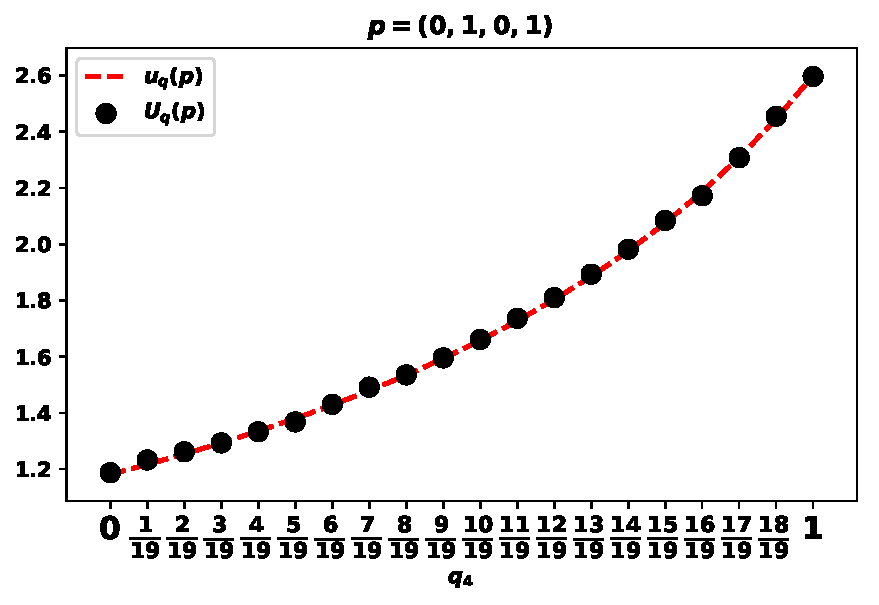
\includegraphics[width=\linewidth]{src/chapters/05/paper/Memory-size-in-the-prisoners-dilemma/img/validation_against_player_one.pdf}
        \end{subfigure}
        \begin{subfigure}{0.45\textwidth}
            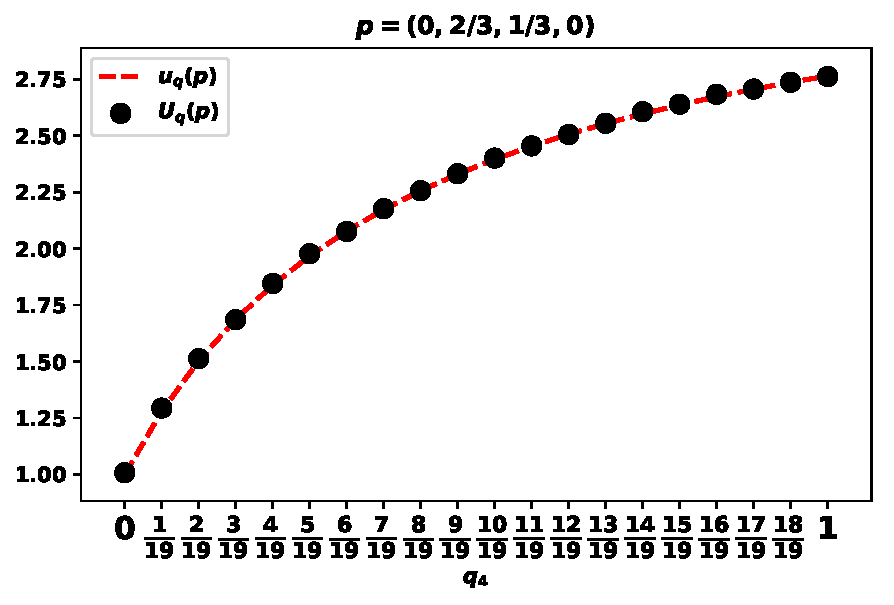
\includegraphics[width=\linewidth]{src/chapters/05/paper/Memory-size-in-the-prisoners-dilemma/img/validation_against_player_two.pdf}
        \end{subfigure}
    \end{center}
    \caption{Simulated and empirical utilities for \(p = (0, 1, 0, 1)\)
    and \(p = (0, \frac{2}{3}, \frac{1}{3}, 0)\) against \((\frac{1}{3}, \frac{1}{3}, \frac{1}{3}, q_4)\) for
    \(q_4 \in \{0,  \frac{1}{19}, \frac{2}{19}, \dots, \frac{18}{19}, 1\}\).
    \(u_q(p)\) is the theoretic value given in Theorem~\ref{theorem:quadratic_form_u},
    and \(U_q(p)\) is simulated numerically.}
    \label{fig:analytical_simulated}
\end{figure}

Theorem~\ref{theorem:quadratic_form_u} can be extended to consider multiple
opponents. The IPD is commonly studied in tournaments and/or Moran Processes
where a strategy interacts with a number of opponents. The payoff of a player in
such interactions is given by the average payoff the player received against
each opponent. More specifically the expected utility of a memory-one strategy
against a \(N\) number of opponents is given by
Theorem~\ref{theorem:tournament_utility}.

\begin{theorem}\label{theorem:tournament_utility}
    The expected utility of a memory-one strategy \(p\in\mathbb{R}_{[0,1]}^4\)
    against a group of opponents \(q^{(1)}, q^{(2)}, \dots, q^{(N)}\), denoted
    as \(\frac{1}{N} \sum\limits_{i=1} ^ {N} {u_q}^{(i)} (p)\), is given by:

    \begin{equation}\label{eq:tournament_utility}
        \frac{1}{N} \sum\limits_{i=1} ^ {N} {u_q}^{(i)} (p) = \frac{1}{N}
        \frac{\sum\limits_{i=1} ^ {N} (\frac{1}{2} pQ^{(i)} p^T + c^{(i)} p + a^ {(i)})
        \prod\limits_{\tiny\begin{array}{l} j=1 \\ j \neq i \end{array}} ^
        N (\frac{1}{2} p\bar{Q}^{(j)} p^T + \bar{c}^{(j)} p + \bar{a}^ {(j)})}
        {\prod\limits_{i=1} ^ N (\frac{1}{2} p\bar{Q}^{(i)} p^T + \bar{c}^{(i)} p + \bar{a}^ {(i)})}.
    \end{equation}
\end{theorem}

The proof of Theorem~\ref{theorem:tournament_utility} is a straightforward algebraic
manipulation.

Similar to the previous result, the formulation of
Theorem~\ref{theorem:tournament_utility} is validated using numerical
simulations where the 10 memory-one strategies described in~\cite{Stewart2012}
have been used as the opponents. Figure~\ref{fig:stewart_plotkin_results} shows
that the simulated behaviour has been captured successfully.

\begin{figure}[!htbp]
    \begin{center}
    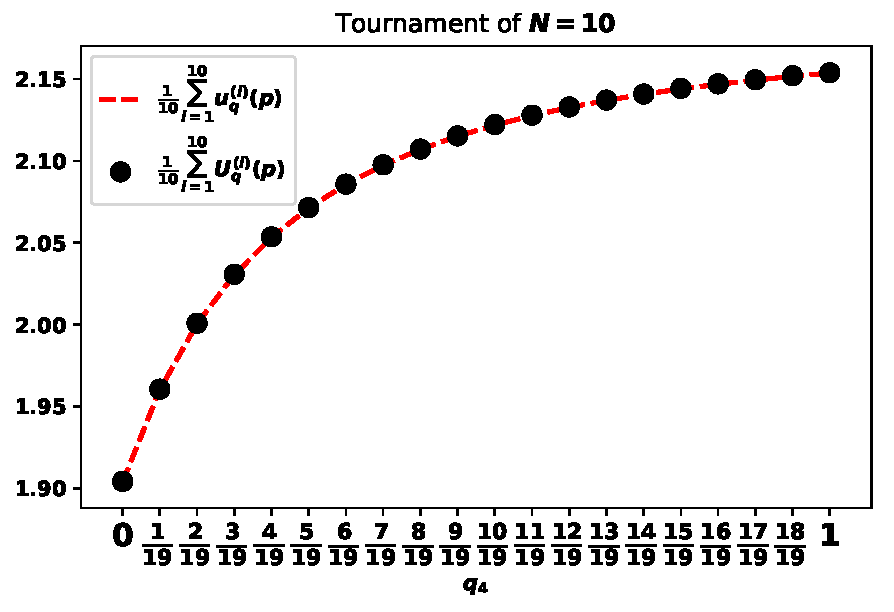
\includegraphics[width=.5\linewidth]{src/chapters/05/paper/Memory-size-in-the-prisoners-dilemma/img/Stewart_tournament_results.pdf}
    \caption{The utilities of memory-one strategies \((\frac{1}{3}, \frac{1}{3}, \frac{1}{3}, p_4)\) for
    \(p_4 \in \{0,  \frac{1}{19}, \frac{2}{19}, \dots, \frac{18}{19}, 1\}\)
    against the 10 memory-one strategies described in~\cite{Stewart2012}.
    \(\frac{1}{10} \sum^{10}_{i=1} u_q^{(i)}(p)\) is the theoretic value given in
    Theorem~\ref{theorem:quadratic_form_u},
    and \(\frac{1}{10} \sum^{10}_{i=1} U_q^{(i)}(p)\) is simulated numerically.}
    \label{fig:stewart_plotkin_results}
    \end{center}
\end{figure}

The list of strategies from~\cite{Stewart2012} was also used to check whether
the utility against a group of strategies could be captured by the utility
against the mean opponent. Thus whether condition (\ref{eq:condition}) holds.
However condition~(\ref{eq:condition}) fails, as shown in
Figure~\ref{fig:hypothesis}.

\begin{equation}\label{eq:condition}
    \frac{1}{N} \sum_{i=1} ^ {N} {u_q}^{(i)} (p) = u_{\frac {1}{N} \sum\limits_{i=1} ^ N q^{(i)}}(p),
\end{equation}

\begin{figure}[!htbp]
    \begin{center}
    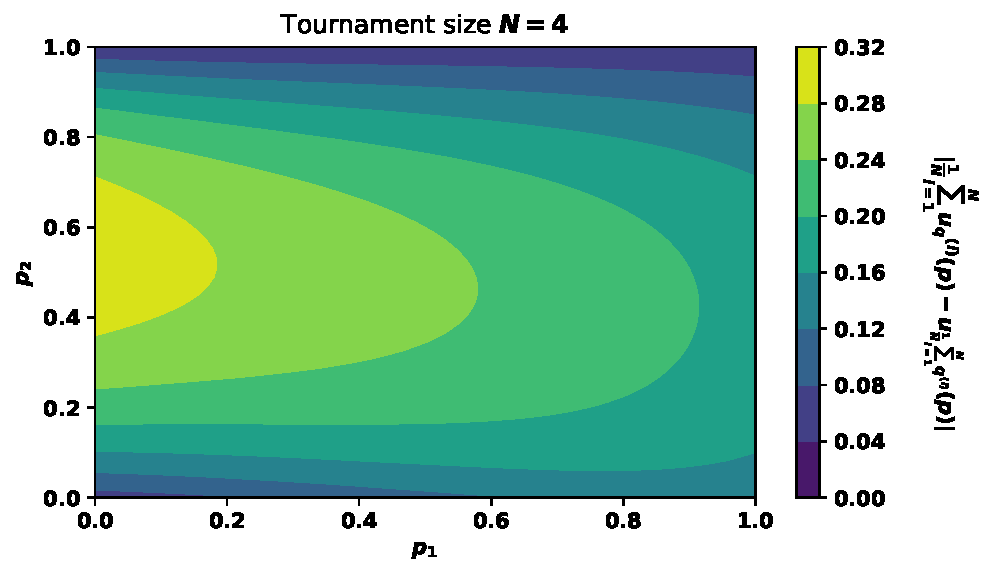
\includegraphics[width=.5\linewidth]{src/chapters/05/paper/Memory-size-in-the-prisoners-dilemma/img/mean_vs_average_heatmap.pdf}
    \end{center}
    \caption{The difference between the average utility against the opponents
    from~\cite{Stewart2012} and the utility against the average player of the
    strategies in~\cite{Stewart2012} of a player \(p=(p_1, p_2, p_1, p_2)\). A
    positive difference indicates that condition (\ref{eq:condition}) does not
    hold.}
    \label{fig:hypothesis}
\end{figure}

Theorem~\ref{theorem:tournament_utility} which allows for the utility of a
memory-one strategy against any number of opponents to be estimated without
simulating the interactions is the main result used in this manuscript. In
Section~\ref{section:best_response_mem_one} it is used to  define best response
memory-one strategies and explore the conditions under which defection dominates
cooperation.

\section{Best responses to memory-one players}\label{section:best_response_mem_one}

This section focuses on best responses and more specifically \textit{memory-one
best response} strategies. A \textit{best response} is a strategy which
corresponds to the most favourable outcome~\cite{Tadelis2013}, thus a memory-one
best response to a set of opponents \(q^{(1)}, q^{(2)}, \dots, q^{(N)}\) corresponds to a strategy \(p^*\) for which
(\ref{eq:tournament_utility}) is maximised. This is considered as a multi
dimensional optimisation problem given by:

\begin{equation}\label{eq:mo_tournament_optimisation}
    \begin{aligned}
    \max_p: & \ \sum_{i=1} ^ {N} {u_q}^{(i)} (p)
    \\
    \text{such that}: & \ p \in \R_{[0, 1]}
    \end{aligned}
\end{equation}

Optimising this particular ratio of quadratic forms is not trivial. It can be
verified empirically for the case of a single opponent that there exists at least
one point for which the definition of concavity does not hold, see Appendix~\ref{appendix:non_concave}
for an example. Some results are
known for non concave ratios of quadratic forms~\cite{Beck2009, Hongyan2014},
however, in these works it is assumed that either both the numerator and the
denominator of the fractional problem are concave or that the denominator is
greater than zero which in this case are not true
(as seen in Theorem~\ref{theorem:concavity}).

\begin{theorem}\label{theorem:concavity}
    The utility of a player \(p\) against an opponent \(q\), \(u_q (p)\), given
    by (\ref{eq:optimisation_quadratic}), is not concave. Furthermore neither
    the numerator or the denominator of (\ref{eq:optimisation_quadratic}), are
    concave or strictly greater than zero.
\end{theorem}

Proof is given in Appendix~\ref{appendix:proof_theorem_three}.

The non concavity of \(u(p)\) indicates multiple local optimal points. The
approach taken here is to introduce a compact way of constructing the candidate
set of all local optimal points, and evaluating which corresponds to the best response
strategy (maximises (\ref{eq:tournament_utility})).

The problem considered is bounded because \(p \in \R^4_{[0, 1]}\).
Therefore, the candidate solutions will exist either at the boundaries of the
feasible solution space, or within that space (the methods of Lagrange
Multipliers~\cite{bertsekas2014} and Karush-Kuhn-Tucker
conditions~\cite{Giorgi2016} are based on this). This approach allow us to
define the best response memory-one strategy to a group of opponents in the
following Lemma:

\begin{lemma}\label{lemma:memone_group_best_response}

    The optimal behaviour of a memory-one strategy player
    \(p^* \in \R_{[0, 1]} ^ 4\)
    against a set of \(N\) opponents \(\{q^{(1)}, q^{(2)}, \dots, q^{(N)} \}\)
    for \(q^{(i)} \in \R_{[0, 1]} ^ 4\) is given by:

    \[p^* = \textnormal{argmax}\sum\limits_{i=1} ^ N  u_q(p), \ p \in S_q.\]

    The set \(S_q\) is defined as all the possible combinations of:

    \begin{equation}\label{eq:s_q_set}
        S_q =
        \left\{p \in \mathbb{R} ^ 4 \left|
            \begin{aligned}
                \bullet\quad p_j \in \{0, 1\} & \quad \text{and} \quad \frac{d}{dp_k} 
                \sum\limits_{i=1} ^ N  u_q^{(i)}(p) = 0
                \quad \text{for all} \quad j \in J \quad \&  \quad k \in K  \quad \text{for all} \quad J, K \\
                & \quad \text{where} \quad J \cap K = \O \quad
                \text{and} \quad J \cup K = \{1, 2, 3, 4\}.\\
                \bullet\quad  p \in \{0, 1\} ^ 4
            \end{aligned}\right.
        \right\}.
    \end{equation}
\end{lemma}

The proof is given in Appendix~\ref{appendix:proof_lemma_four}.

Note that there is no immediate way to find the zeros of \(\frac{d}{dp} \sum\limits_{i=1} ^ N  u_q(p)\);

{\small
\begin{align}\label{eq:mo_tournament_derivative}
    \frac{d}{dp} \sum\limits_{i=1} ^ {N} {u_q}^{(i)} (p) & = \nonumber \\
    & =  \displaystyle\sum\limits_{i=1} ^ {N}
    \frac{\left(pQ^{(i)} + c^{(i)}\right) \left(\frac{1}{2} p\bar{Q}^{(i)} p^T + \bar{c}^{(i)} p + \bar{a}^ {(i)}\right)
    - \left(p\bar{Q}^{(i)} + \bar{c}^{(i)}\right) \left(\frac{1}{2} pQ^{(i)} p^T + c^{(i)} p + a^ {(i)}\right)}
    {\left(\frac{1}{2} p\bar{Q}^{(i)} p^T + \bar{c}^{(i)} p + \bar{a}^ {(i)}\right)^ 2}
\end{align}
}

For \(\frac{d}{dp} \sum\limits_{i=1} ^ N  u_q(p)\) to equal zero then:

{\scriptsize
\begin{align}\label{eq:polynomials_roots}
    \displaystyle\sum\limits_{i=1} ^ {N} \left(
    \left(pQ^{(i)} + c^{(i)}\right) \left(\frac{1}{2} p\bar{Q}^{(i)} p^T + \bar{c}^{(i)} p + \bar{a}^ {(i)}\right)
    - \left(p\bar{Q}^{(i)} + \bar{c}^{(i)}\right) \left(\frac{1}{2} pQ^{(i)} p^T + c^{(i)} p + a^ {(i)}\right)\right)
    &= 0, \quad {while} \\
    \displaystyle\sum\limits_{i=1} ^ {N} \frac{1}{2} p\bar{Q}^{(i)} p^T + \bar{c}^{(i)} p + \bar{a}^ {(i)} &\neq 0.
\end{align}}

Finding best response memory-one strategies, more specifically constructing the
subset \(S_q\), can be done analytically. The points for any or all of \(p_i \in
\{0, 1\}\) for \(i \in \{1, 2, 3, 4\}\) are trivial, and finding the
roots of the partial derivatives which are a set of polynomials of equations
(\ref{eq:polynomials_roots}) is feasible using resultant
theory~\cite{Jonsson2005}; however, for large systems building the resultant quickly becomes
intractable. As a result, a numerical method taking advantage of the structure
will be used for finding best response memory-one strategies. This will be described
in Section~\ref{section:numerical_experiments}. The rest of
the section focuses on an immediate theoretical result from
Lemma~\ref{lemma:memone_group_best_response}.

\subsection{Stability of defection}\label{subsection:stability_of_defection}

An immediate result from Lemma~\ref{lemma:memone_group_best_response} can be
obtained by evaluating the sign of the derivative
(\ref{eq:mo_tournament_derivative}) at \(p=(0, 0, 0, 0)\). If at that point the
derivative is negative, then the utility of a player only decreases if they were
to change their behaviour, and thus defection at that point is stable.

\begin{lemma}\label{lemma:stability_of_defection}
    In a tournament of \(N\) players \(\{q^{(1)}, q^{(2)}, \dots, q^{(N)} \}\)
    for \(q^{(i)} \in \R_{[0, 1]} ^ 4\)
    defection is stable if the transition probabilities of the
    opponents satisfy conditions (\ref{eq:defection_condition_one}) and (\ref{eq:defection_condition_two}).

    \begin{equation}\label{eq:defection_condition_one}
        \sum_{i=1} ^ N (c^{(i)T} \bar{a}^{(i)} - \bar{c}^{(i)T} a^{(i)}) \leq 0
    \end{equation}

    while,

    \begin{equation}\label{eq:defection_condition_two}
        \sum_{i=1} ^ N \bar{a}^{(i)} \neq 0
    \end{equation}
\end{lemma}

\begin{proof}
    For defection to be stable the derivative of the utility
    at the point \(p = (0, 0, 0, 0)\) must be negative. This would indicate that
    the utility function is only declining from that point onwards.

    Substituting \(p = (0, 0, 0, 0)\) in
    equation~(\ref{eq:mo_tournament_derivative}) gives:

    \begin{equation}
    \sum_{i=1} ^ N \frac{(c^{(i)T} \bar{a}^{(i)} - \bar{c}^{(i)T} a^{(i)})}
    {(\bar{a}^{(i)})^2}
    \end{equation}

    The sign of the numerator \( \displaystyle\sum_{i=1} ^ N (c^{(i)T} \bar{a}^{(i)} - \bar{c}^{(i)T} a^{(i)})\)
    can vary based on the transition probabilities of the opponents.
    The denominator can not be negative, and otherwise is always positive.
    Thus the sign of the derivative is negative if and only if
    \( \displaystyle\sum_{i=1} ^ N (c^{(i)T} \bar{a}^{(i)} - \bar{c}^{(i)T} a^{(i)}) \leq 0\).
\end{proof}

Consider a population for which defection is known to be stable. In that
population all the members will over time adopt the same behaviour; thus in such
population cooperation will never take over. This is demonstrated in
Figures~\ref{fig:stable_defection} and~\ref{fig:unstable_defection}.

Lemma~\ref{lemma:stability_of_defection} gives a condition under which cooperation
cannot occur and is the last theoretical result
presented in this manuscript. The following section focuses on numerical
experiments.

\begin{figure}[!htb]
    \begin{subfigure}{0.49\textwidth}
        \centering
        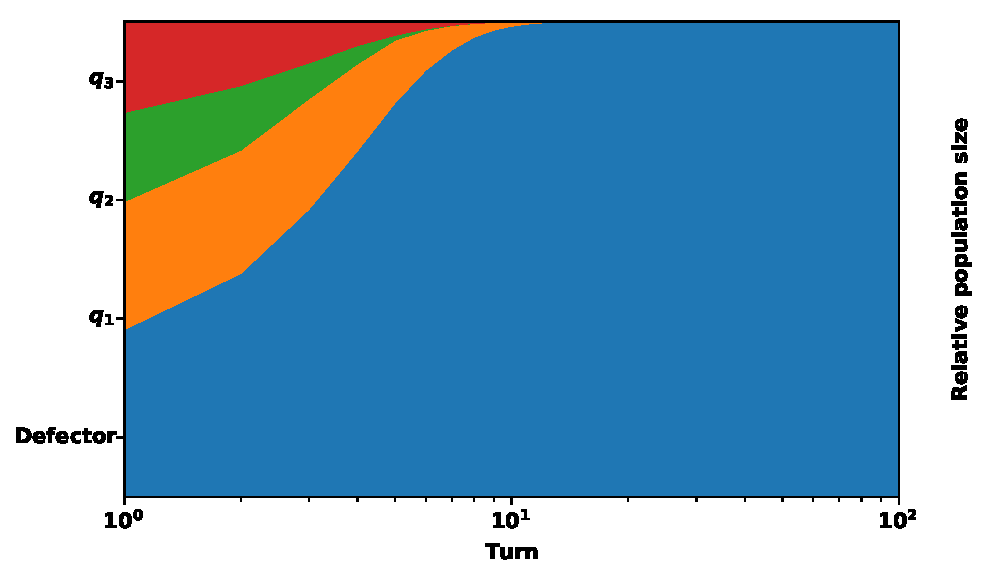
\includegraphics[width=\linewidth]{src/chapters/05/paper/Memory-size-in-the-prisoners-dilemma/img/population_defection_takes_over.pdf}
        \caption{For opponents \(q_{1}=(\frac{371}{1250},\frac{4693}{25000},\frac{4037}{50000},\frac{18461}{25000})\),
        $q_{2}=(\frac{48841}{100000},\frac{30587}{50000},\frac{76591}{100000},\frac{25921}{50000})$ and
        $q_{3}=(\frac{22199}{100000},\frac{87073}{100000},\frac{646}{3125},\frac{91861}{100000})$
        conditions (\ref{eq:defection_condition_one}) and
        (\ref{eq:defection_condition_two}) hold and Defector takes over the
        population.}
        \label{fig:stable_defection}
    \end{subfigure}\hfill
    \begin{subfigure}{0.49\textwidth}
        \centering
        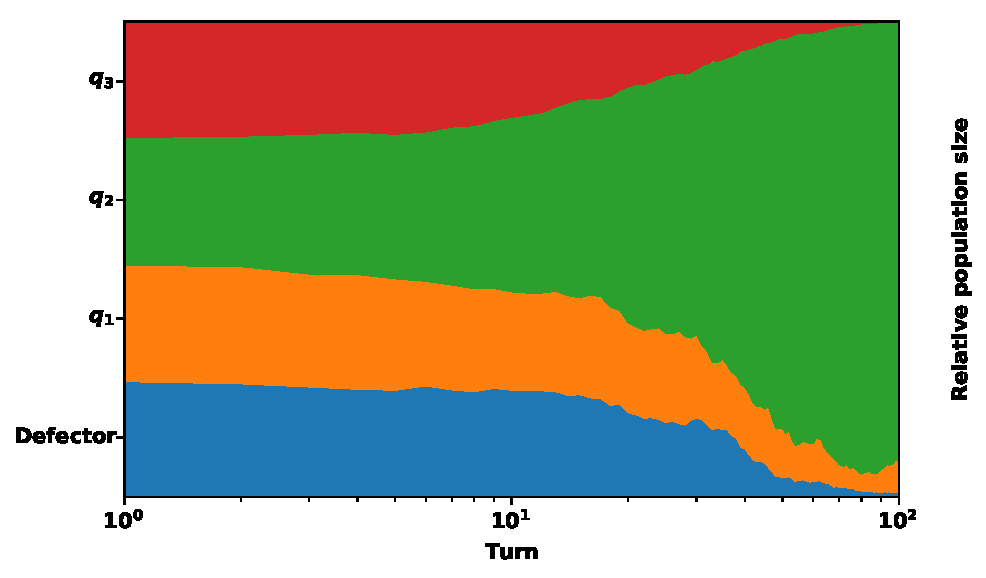
\includegraphics[width=\linewidth]{src/chapters/05/paper/Memory-size-in-the-prisoners-dilemma/img/population_defection_fails.pdf}
        \caption{For opponents $q_{1}=(\frac{69773}{100000},\frac{21609}{100000},\frac{97627}{100000},\frac{623}{100000})$,
        $q_{2}=(\frac{12649}{50000},\frac{43479}{100000},\frac{38969}{50000},\frac{19769}{100000})$ and
        $q_{3}=(\frac{96703}{100000},\frac{54723}{100000},\frac{24317}{25000},\frac{35741}{50000})$
        (\ref{eq:defection_condition_one}) fails and
        (\ref{eq:defection_condition_two}) holds and Defector does not take over
        the population.}
        \label{fig:unstable_defection}
    \end{subfigure}
\end{figure}

\section{Numerical experiments} \label{section:numerical_experiments}

The results of this section rely on estimating best response memory-one strategies, but as stated in
Section~\ref{section:best_response_mem_one}, estimating best responses
analytically can quickly become an intractable problem. As a result, best
responses will be estimated heuristically using Bayesian
optimisation~\cite{Mokus1978}. Bayesian optimisation is a global optimisation
algorithm that has proven to outperform many other popular
algorithms~\cite{Jones2001}. The algorithm builds a bayesian understanding of
the objective function which is well suited to the potential multiple local optimas in
the described search space of this work. Differential evolution~\cite{Storn1997}
was also considered, however, it was not selected due to Bayesian optimisation being
computationally more efficient.

As an example of the algorithm's usage let us consider the optimisation problem
of (\ref{eq:mo_tournament_optimisation}). Figure~\ref{bayesian_example}
illustrates the change of the utility function over iterations of the algorithm.
The algorithm is set to run for 60 iterations. After 60 iterations if the
utility has changed in the last 10\% iterations then algorithm runs for a
further 20 iterations. This is repeated until there is no change to the utility
in the last 10\% of iterations.


\begin{figure}[!htbp]
    \begin{center}
    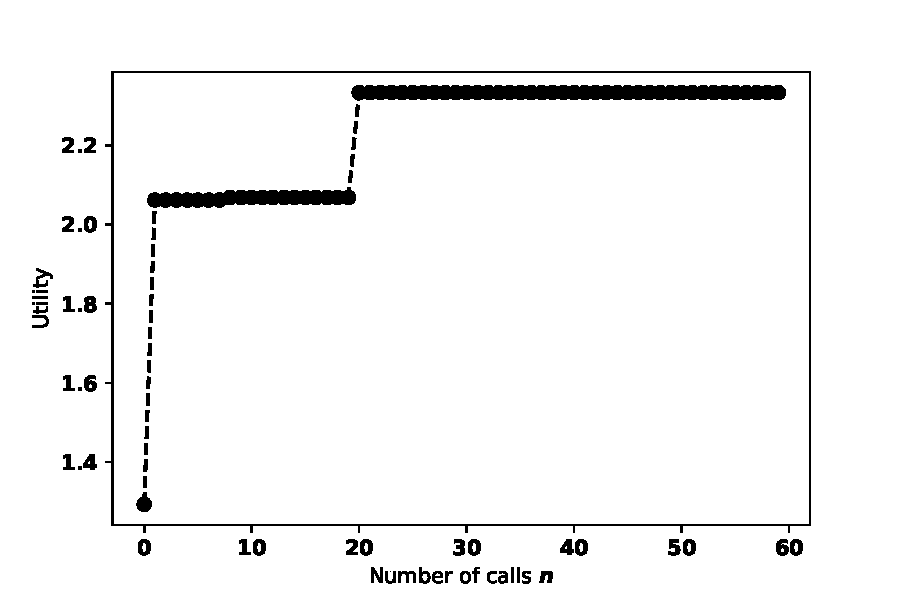
\includegraphics[width=.5\linewidth]{src/chapters/05/paper/Memory-size-in-the-prisoners-dilemma/img/bayesian_example.pdf}
    \end{center}
    \caption{Utility over time of calls using Bayesian optimisation. The
    opponents are \(q^{(1)} = (\frac{1}{3}, \frac{1}{3}, \frac{1}{3},
    \frac{1}{3})\) and \(q^{(2)} = (\frac{1}{3}, \frac{1}{3},
    \frac{1}{3}, \frac{1}{3})\). The best response obtained is \(p^* = (0, \frac{11}{50}, 0, 0)\)}
    \label{bayesian_example}
\end{figure}

The rest of the section is structured as follows. In
Section~\ref{subsection:best_response_n_2}, Bayesian optimisation is used to
generate a data set containing memory-one best responses against a number of
random opponents. The extortionate behaviour of these best responses is then
evaluated using a method introduced in~\cite{Knight2019}. In Section
\ref{subsection:best_respnse_evolutionary_setting}, a similar data set and
approach is discussed but this time the best responses are memory-one best
responses in an evolutionary setting where they also incorporate self
interactions. This has immediate applications to Moran processes.
Finally, Section~\ref{subsection:longer_memory_best_response}
compares the performances of memory-one and longer-memory best responses against
a number of opponents.

\subsection{Best response memory-one strategies for \(N=2\)}\label{subsection:best_response_n_2}

As briefly discussed in Section~\ref{section:introduction}, zero-determinants
have been praised for their robustness against a single opponent.
Zero-determinants are evidence that extortion works in pairwise interactions,
their behaviour ensures that the strategies will
never lose a game. However, this paper
argues that in multi opponent interactions, where the payoffs matter, strategies
trying to exploit their opponents will suffer.

Compared to zero-determinants, best response memory-one strategies which
have a theory of mind of their opponents, utilise their behaviour in order to
gain the most from their interactions. The question that arises then is whether
best response strategies are optimal because they behave in an extortionate
way. To estimate a strategy's extortionate
behaviour the SSE method as described in~\cite{Knight2019} is used. SSE is
defined as how far a strategy is from behaving extortionate, thus a high
SSE implies a non extortionate behaviour.

%TODO include explanation of SSE

A data set of best response memory-one strategies with \(N=2\) opponents has been
generated which is available at~\cite{glynatsi2019}. The data set contains a total of 1000 trials
corresponding to 1000 different instances of a best response strategy. For each
trial a set of 2 opponents is randomly generated and the memory-one best response
against them is found. The probabilities \(q_i\) of the opponents are
randomly generated and Figures~\ref{fig:first_opponents_probabilities} and
\ref{fig:second_opponents_probabilities}, show that they are uniformly
distributed over the trials. Thus, the full space of possible opponents has been
covered.

\begin{figure}[!htbp]
    \begin{subfigure}{0.49\textwidth}
        \centering
        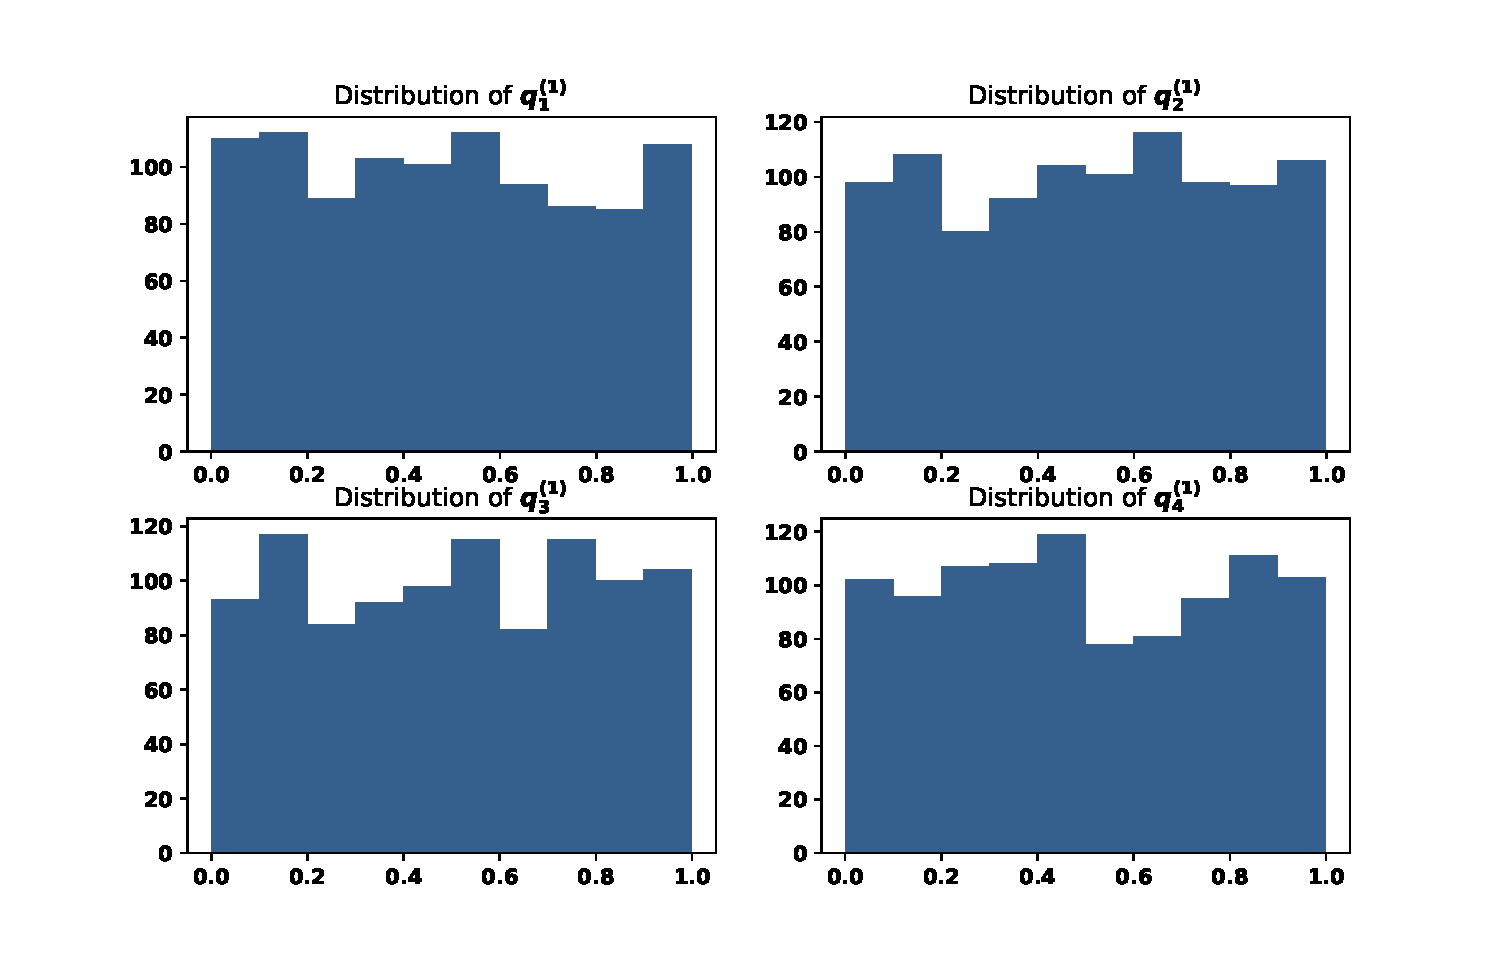
\includegraphics[width=\linewidth]{src/chapters/05/paper/Memory-size-in-the-prisoners-dilemma/img/first_opponent_probabilities.pdf}
        \subcaption{Distributions of first opponents' probabilities.}
        \label{fig:first_opponents_probabilities}
    \end{subfigure}
    \begin{subfigure}{0.49\textwidth}
        \centering
        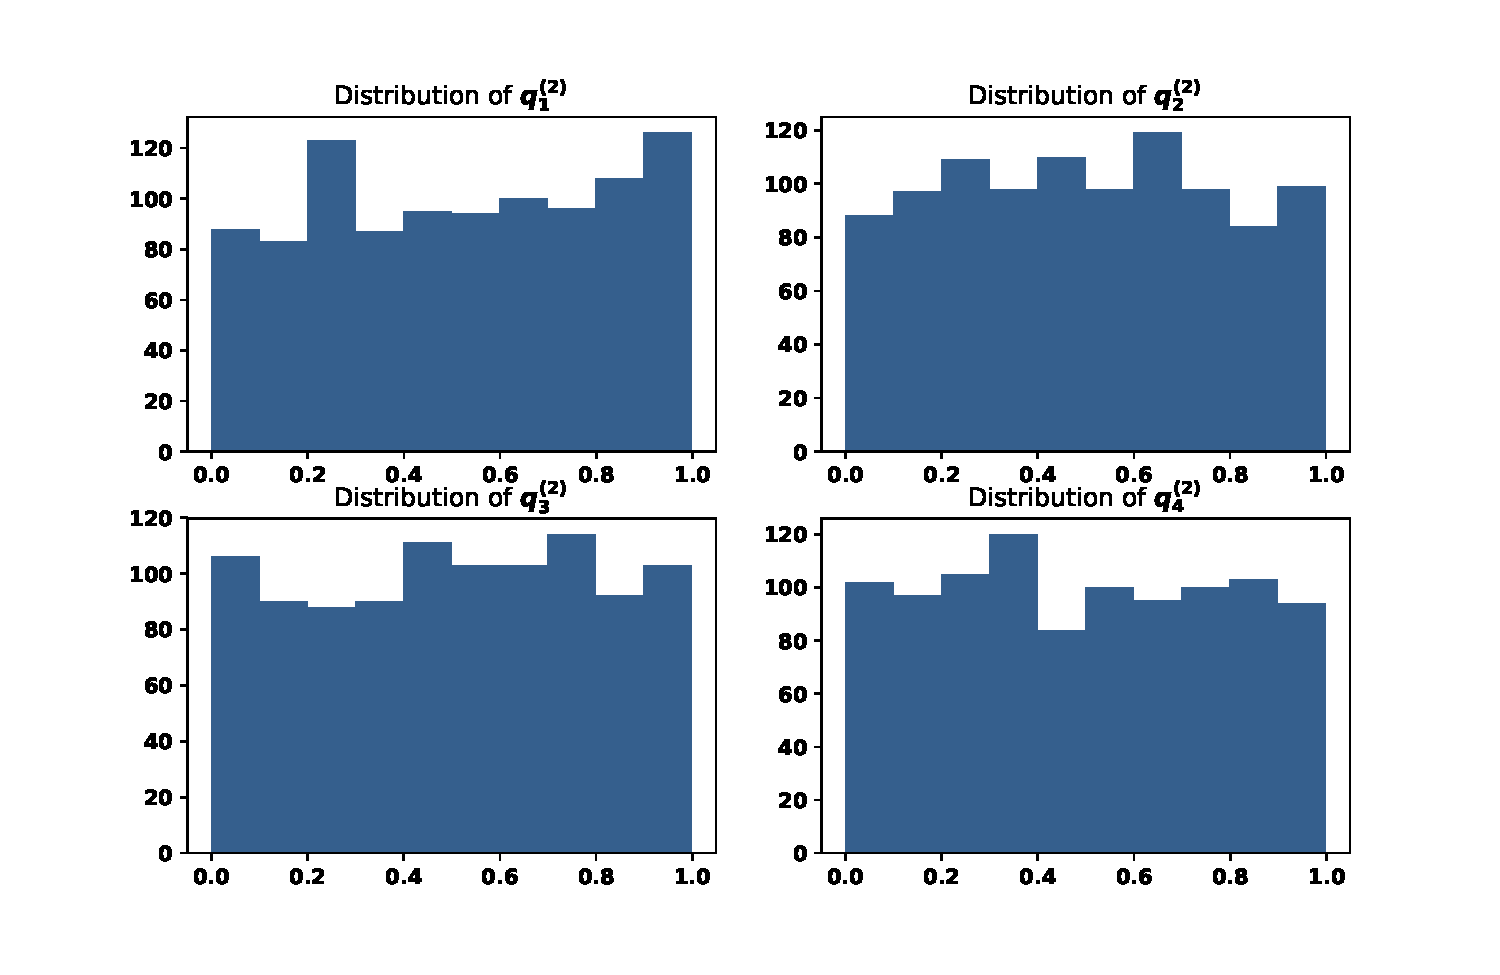
\includegraphics[width=\linewidth]{src/chapters/05/paper/Memory-size-in-the-prisoners-dilemma/img/second_opponent_probabilities.pdf}
        \subcaption{Distributions of second opponents' probabilities.}
        \label{fig:second_opponents_probabilities}
    \end{subfigure}
\end{figure}

The SSE method has been applied to the data set. The distribution of SSE for the best response is given in
Figure~\ref{fig:sserror_mem_one} and a statistics summary in
Table~\ref{table:sserror_stats}. The distribution of SSE is skewed to the left,
indicating that the best response does exhibit extortionate behaviour, however,
the best response is not uniformly extortionate. A positive measure of skewness
and kurtosis indicates a heavy tail to the right. Therefore, in several cases the
strategy is not trying to extort its the opponents.

So although the best response strategy can exhibit extortionate behaviour, its
performance is maximised by behaving in a more adaptable way than zero-determinant
strategies. This is confirms similar results such as~\cite{Knight2019}.
This analysis will now be extended to an evolutionary setting.

\begin{figure}[!htbp]
    \begin{minipage}{0.72\textwidth}
            \begin{center}
                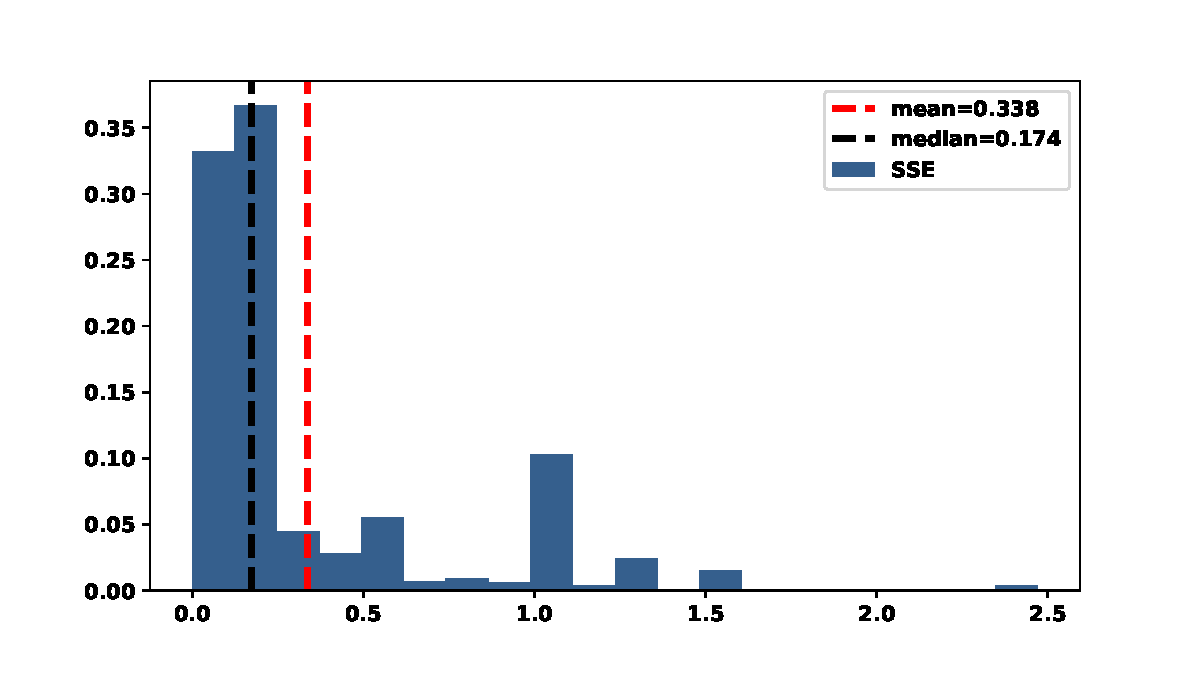
\includegraphics[width=\linewidth]{src/chapters/05/paper/Memory-size-in-the-prisoners-dilemma/img/best_respones_sserror.pdf}
            \end{center}
                \caption{Distribution of SSE for memory-one best responses, when \(N=2\).}
                \label{fig:sserror_mem_one}
    \end{minipage}\hspace{1cm}
    \begin{minipage}{0.21\textwidth}
        \centering
        \captionsetup{type=table}
        \resizebox{.85\columnwidth}{!}{%
            \begin{tabular}{lr}
\toprule
{} &     SSE \\
\midrule
count  &  1000.00000 \\
mean   &     0.33762 \\
std    &     0.39667 \\
min    &     0.00000 \\
5\%     &     0.02078 \\
25\%    &     0.07597 \\
50\%    &     0.17407 \\
95\%    &     1.05943 \\
max    &     2.47059 \\
median &     0.17407 \\
skew   &     1.87231 \\
kurt   &     3.60029 \\
\bottomrule
\end{tabular}
}
            \caption{Summary statistics SSE of best response memory one strategies included
            tournaments of \(N=2\).}
            \label{table:sserror_stats}
      \end{minipage}
\end{figure}

\subsection{Memory-one best responses in evolutionary dynamics}\label{subsection:best_respnse_evolutionary_setting}

As mentioned in Section~\ref{section:utility}, the IPD is commonly studied in
Moran processes, and generally, in evolutionary processes. In these settings self
interactions are key. This section extends the formulation of best responses
in evolutionary dynamics, more specifically, the optimisation problem of
(\ref{eq:mo_tournament_optimisation}) is extended to
include self interactions.

Self interactions can be incorporated in the formulation
that has been used so far. The utility is given by,

\begin{equation}
    \frac{1}{N} \sum\limits_{i=1} ^ {N} {u_q}^{(i)} (p) + u_p(p)
\end{equation}

and the optimisation problem of (\ref{eq:mo_tournament_optimisation}) is modified to give:

\begin{equation}\label{eq:mo_evolutionary_optimisation}
    \begin{aligned}
    \max_p: & \ \frac{1}{N} \sum\limits_{i=1} ^ {N} {u_q}^{(i)} (p) + u_p(p)
    \\
    \text{such that}: & \ p \in \R_{[0, 1]}
    \end{aligned}
\end{equation}

% Note that exact formulate are known for given evolutionary processes, however,
% for simplicity 17 is given to optimisation.
For determining the memory-one best response in an evolutionary setting,
an algorithmic approach is considered, called \textit{best
response dynamics}. Best response dynamics are commonly used in evolutionary
game theory. They represent a class of strategy updating rules, where players in
the next round are determined by their best responses to some subset of the
population. The best response dynamics approach used in this manuscript is given by
Algorithm~\ref{algo:best_response_dynamics}.

\begin{minipage}{.6\textwidth}
    \begin{algorithm}[H]
        $p^{(t)}\leftarrow (1, 1, 1, 1)$\;
        \While{$p^{(t)} \neq p ^{(t -1)}$}{
         $p^{(t + 1)} =  \text{argmax} \frac{1}{N} \sum\limits_{i=1} ^ {N} {u_q}^{(i)}
         (p^{(t + 1)}) + u_p^{(t)}(p^{(t + 1)})$\;
        }
        \caption{Best response dynamics Algorithm}
        \label{algo:best_response_dynamics}
    \end{algorithm}
\end{minipage}

The best response dynamics algorithm starts by setting an initial
solution \(p^{(1)}=(1, 1, 1, 1)\), and repeatedly finds a strategy that maximises
(\ref{eq:mo_evolutionary_optimisation}) using Bayesian optimisation. The
algorithm stops once a cycle (a sequence of iterated evaluated points) is
detected. A numerical example of the algorithm is given in Figure~\ref{fig:best_response_dynamics_results}.

\begin{figure}[!htbp]
    \centering
    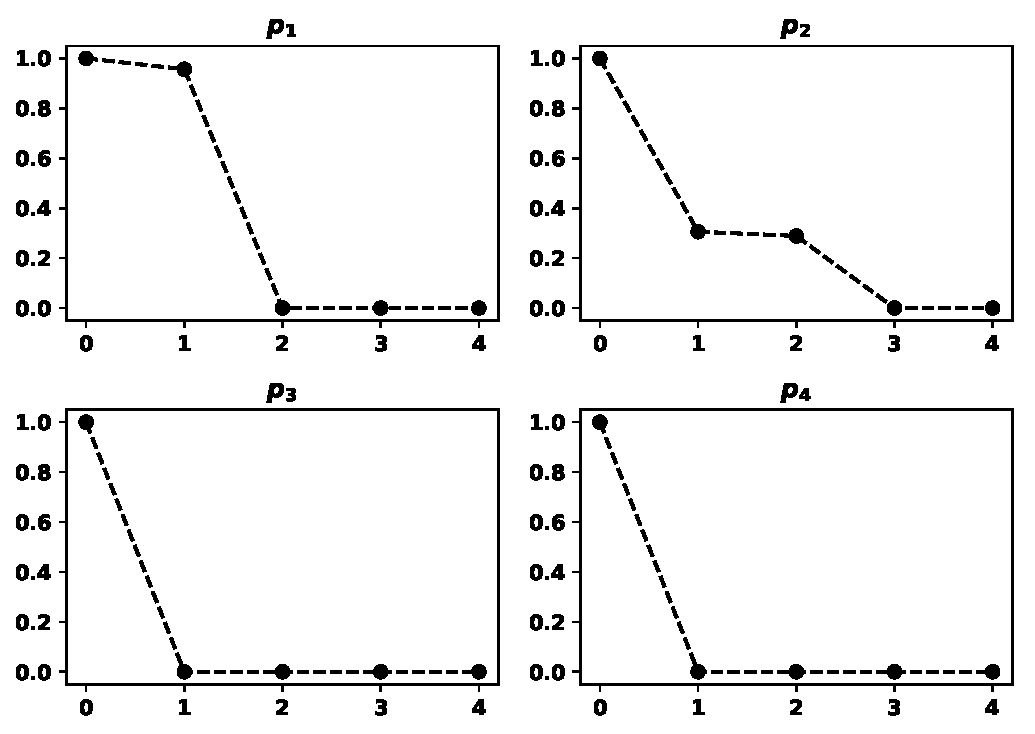
\includegraphics[width=.6\textwidth]{src/chapters/05/paper/Memory-size-in-the-prisoners-dilemma/img/evolution_example_two.pdf}
    \caption{Best response dynamics with \(N=2\). More specifically, for
    \(q ^{(1)}=(\frac{59}{250},
                \frac{1031}{10000},
                \frac{99}{250},
                \frac{1549}{10000})\) and
    \(q ^{(2)}=(\frac{133}{2000},
                \frac{803}{2000},
                \frac{9179}{10000},
                \frac{2001}{2500})\).}
\label{fig:best_response_dynamics_results}
\end{figure}

The algorithm has been used to estimate the best response in an evolutionary
setting for each of the 1000 pairs of opponents described in
Section~\ref{subsection:best_response_n_2}. These are also included in the data
set~\cite{glynatsi2019}, and moreover, the SSE method has also been applied. The
distribution of SSE is given by Figure~\ref{fig:sserror_mem_one} and a
statistical summary by Table~\ref{table:sserror_stats}.

Similarly to the results of Section~\ref{subsection:best_response_n_2}, the
evolutionary best response strategy does not behave uniformly extortionately. A
larger value of both the kurtosis and the skewness of the SSE distribution
indicates that in evolutionary settings a memory-one best response is even more
adaptable.

The difference between best responses in tournaments and in evolutionary
settings are further explored by Figure~\ref{fig:behaviour_violin_plots}.
Though, Table~\ref{table:wilcoxon_tests} details that no statistically
significant differences has been found, from
Figure~\ref{fig:behaviour_violin_plots}, it seems that evolutionary best
response has a higher $p_2$ median. Thus, they more likely to forgive after
being tricked.

\begin{figure}[!htbp]
    \begin{minipage}{0.72\textwidth}
            \begin{center}
            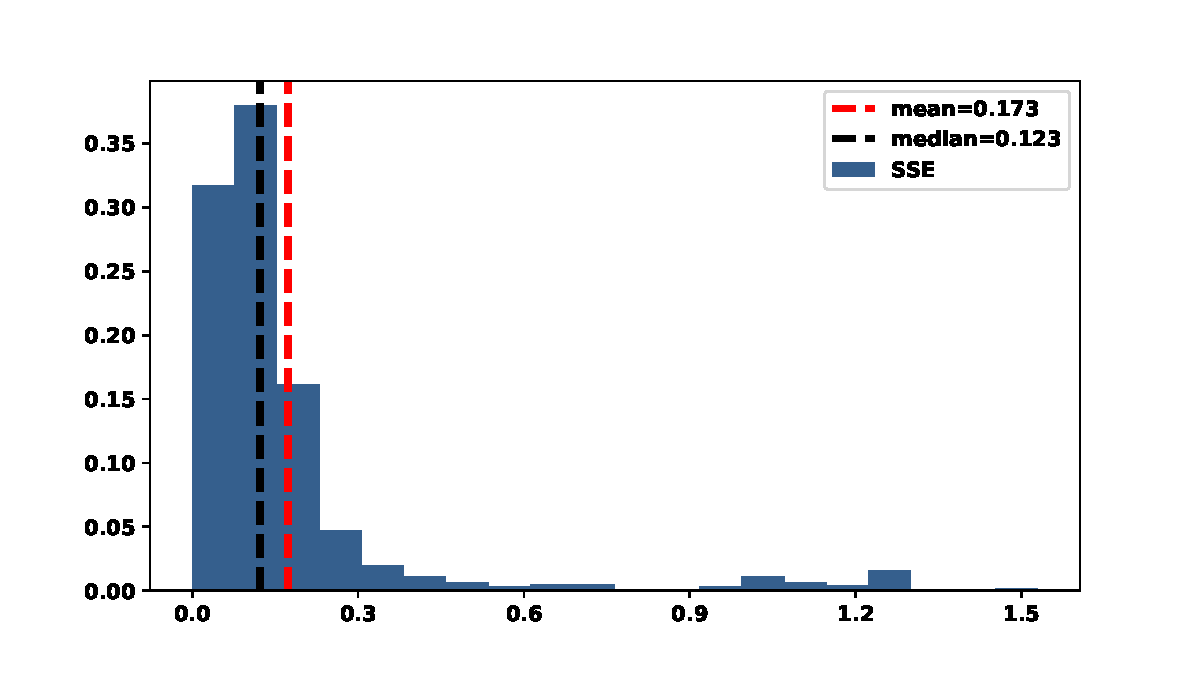
\includegraphics[width=\linewidth]{src/chapters/05/paper/Memory-size-in-the-prisoners-dilemma/img/evo_sserror.pdf}
            \end{center}
            \caption{Distribution of SSE of best response memory-one strategies in
            evolutionary settings, when \(N=2\).}
            \label{fig:sserror_mem_one}
    \end{minipage}\hspace{1cm}
    \begin{minipage}{0.21\textwidth}
        \centering
        \captionsetup{type=table}
        \resizebox{.85\columnwidth}{!}{%
            \begin{tabular}{lr}
\toprule
{} &  SSE \\
\midrule
count  &    1000.00000 \\
mean   &       0.17326 \\
std    &       0.23489 \\
min    &       0.00001 \\
5\%     &       0.01497 \\
25\%    &       0.05882 \\
50\%    &       0.12253 \\
95\%    &       0.67429 \\
max    &       1.52941 \\
median &       0.12253 \\
skew   &       3.41839 \\
kurt   &      11.92339 \\
\bottomrule
\end{tabular}
}
            \caption{Summary statistics SSE of best response memory-one strategies in
            evolutionary settings, when when \(N=2\).}
            \label{table:sserror_stats}
      \end{minipage}
\end{figure}

\begin{figure}[!htbp]
    \centering
    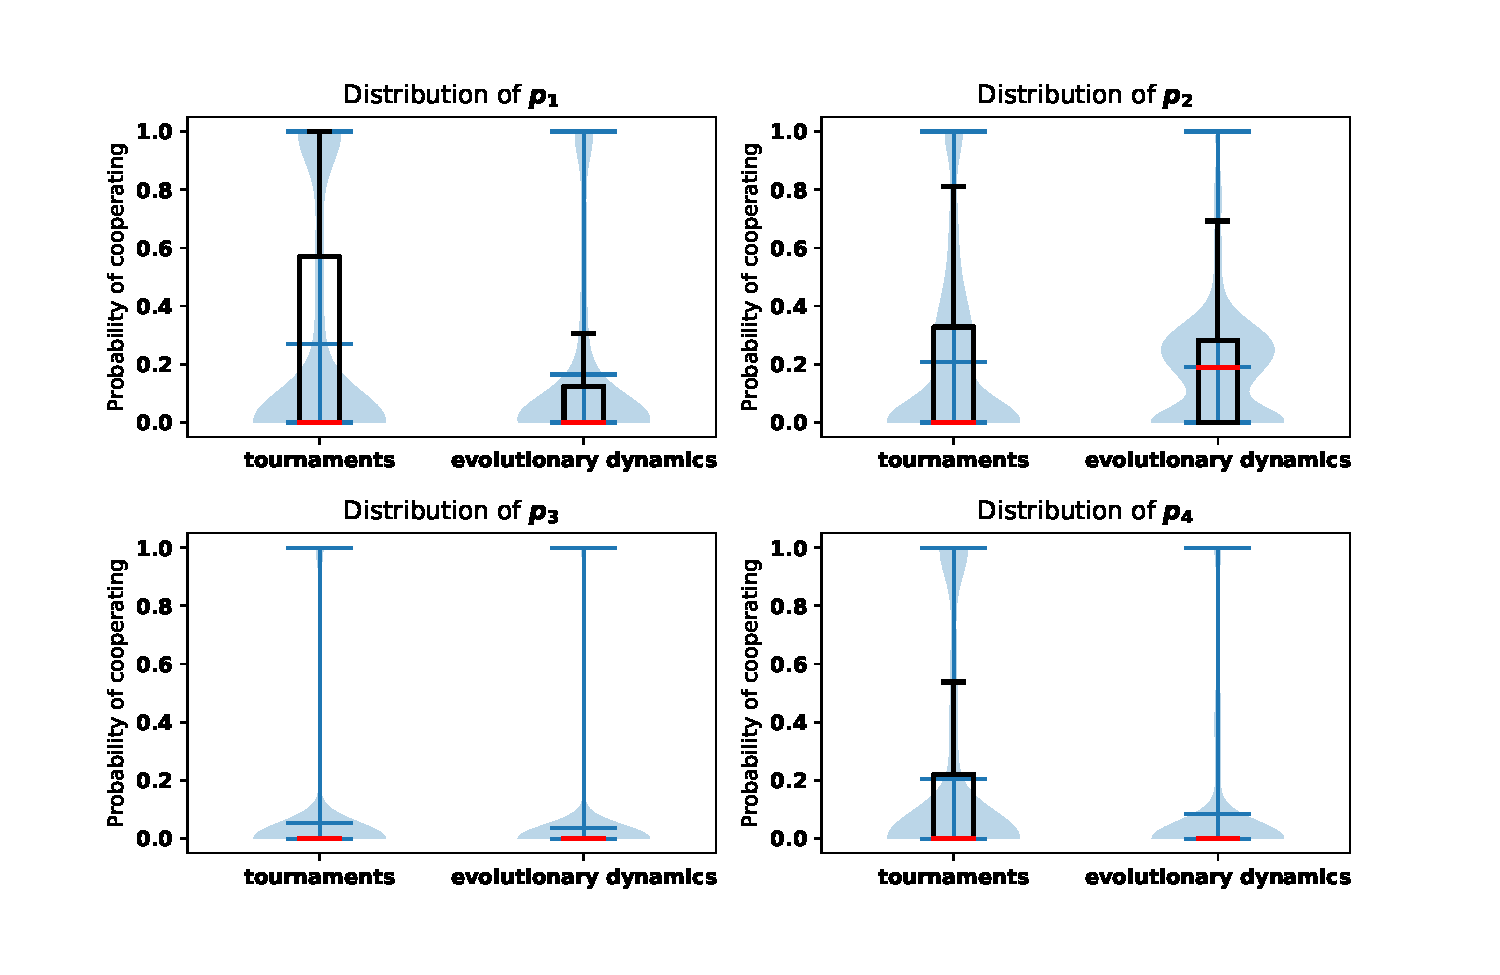
\includegraphics[width=.8\textwidth]{src/chapters/05/paper/Memory-size-in-the-prisoners-dilemma/img/behaviour_violin_plots.pdf}
    \caption{Distributions of \(p^*\) for both best response and evolutionary memory-one
    strategies.}
    \label{fig:behaviour_violin_plots}
\end{figure}

\begin{table}[!htbp]
    \centering
    \resizebox{.7\columnwidth}{!}{%
    \begin{tabular}{llrrr}
\toprule
{} & Best Response Median in: &  Tournament &  Evolutionary Settings &  p-values \\
\midrule
&       Distribution $p_1$ &         0.0 &                0.00000 &       0.0 \\
&       Distribution $p_2$ &         0.0 &                0.19847 &       0.0 \\
&       Distribution $p_3$ &         0.0 &                0.00000 &       0.0 \\
&       Distribution $p_4$ &         0.0 &                0.00000 &       0.0 \\
\bottomrule
\end{tabular}
}
    \caption{A non parametric test, Wilcoxon Rank Sum, has been performed to
    tests the difference in the median values of the cooperation probabilities
    in tournaments versus evolutionary settings. A non parametric test is used because
    is evident that the data are skewed.}\label{table:wilcoxon_tests}
\end{table}

\subsection{Longer memory best response}\label{subsection:longer_memory_best_response}

This section focuses on the memory size of strategies. The effectiveness of
memory in the IPD has been previously explored in the literature, as
discussed in Section~\ref{section:introduction}, however, none of the
previous works has compared the performance of longer-memory strategies to
memory-one best responses.

In~\cite{Harper2017}, a strategy called \textit{Gambler} which makes
probabilistic decisions based on the opponent's \(n_1\) first moves, the
opponent's \(m_1\) last moves and the player's \(m_2\) last moves was
introduced. In this manuscript Gambler with parameters: $n_1 = 2, m_1 = 1$ and $m_2 = 1$ is used
as a longer-memory strategy.

By considering the opponent's first two moves, the opponents last move and the
player's last move, there are only 16 $(4 \times 2 \times 2)$ possible outcomes
that can occur, furthermore, Gambler also makes a probabilistic decision of
cooperating in the opening move. Thus, Gambler is a function \(f: \{\text{C,
D}\} \rightarrow [0, 1]_{\R}\). This can be hard coded as an element
of \([0, 1]_{\R} ^ {16 + 1}\), one probability for each outcome plus the opening
move. Hence, compared to (\ref{eq:mo_tournament_optimisation}), finding an
optimal Gambler is a 17 dimensional problem given by:

\begin{equation}\label{eq:gambler_optimisation}
    \begin{aligned}
    \max_p: & \ \sum_{i=1} ^ {N} {U_q}^{(i)} (f)
    \\
    \text{such that}: & \ f \in \R_{[0, 1]}^{17}
    \end{aligned}
\end{equation}

Note that (\ref{eq:tournament_utility}) can not be used here for the utility
of Gambler, and actual simulated players are used. This is done using~\cite{axelrodproject}
with 500 turns and 200 repetitions, moreover, (\ref{eq:gambler_optimisation})
is solved numerically using Bayesian optimisation.

Similarly to previous sections, a large data set has been generated with
instances of an optimal Gambler and a memory-one best response, available
at~\cite{glynatsi2019}. Estimating a best response Gambler (17 dimensions) is
computational more expensive compared to a best response memory-one (4
dimensions). As a result, the analysis of this section is based on a total of
130 trials. For each trial two random opponents have been selected. The 130 pair
of opponents are a sub set of the opponents used in
Section~\ref{subsection:best_response_n_2}-
\ref{subsection:best_respnse_evolutionary_setting}. The distributions of their
transition probabilities are given in Figures
\ref{fig:first_opponents_probabilities_with_gambler} and
\ref{fig:first_opponents_probabilities_with_gambler}.

\begin{figure}[!htbp]
    \begin{subfigure}{0.49\textwidth}
        \centering
        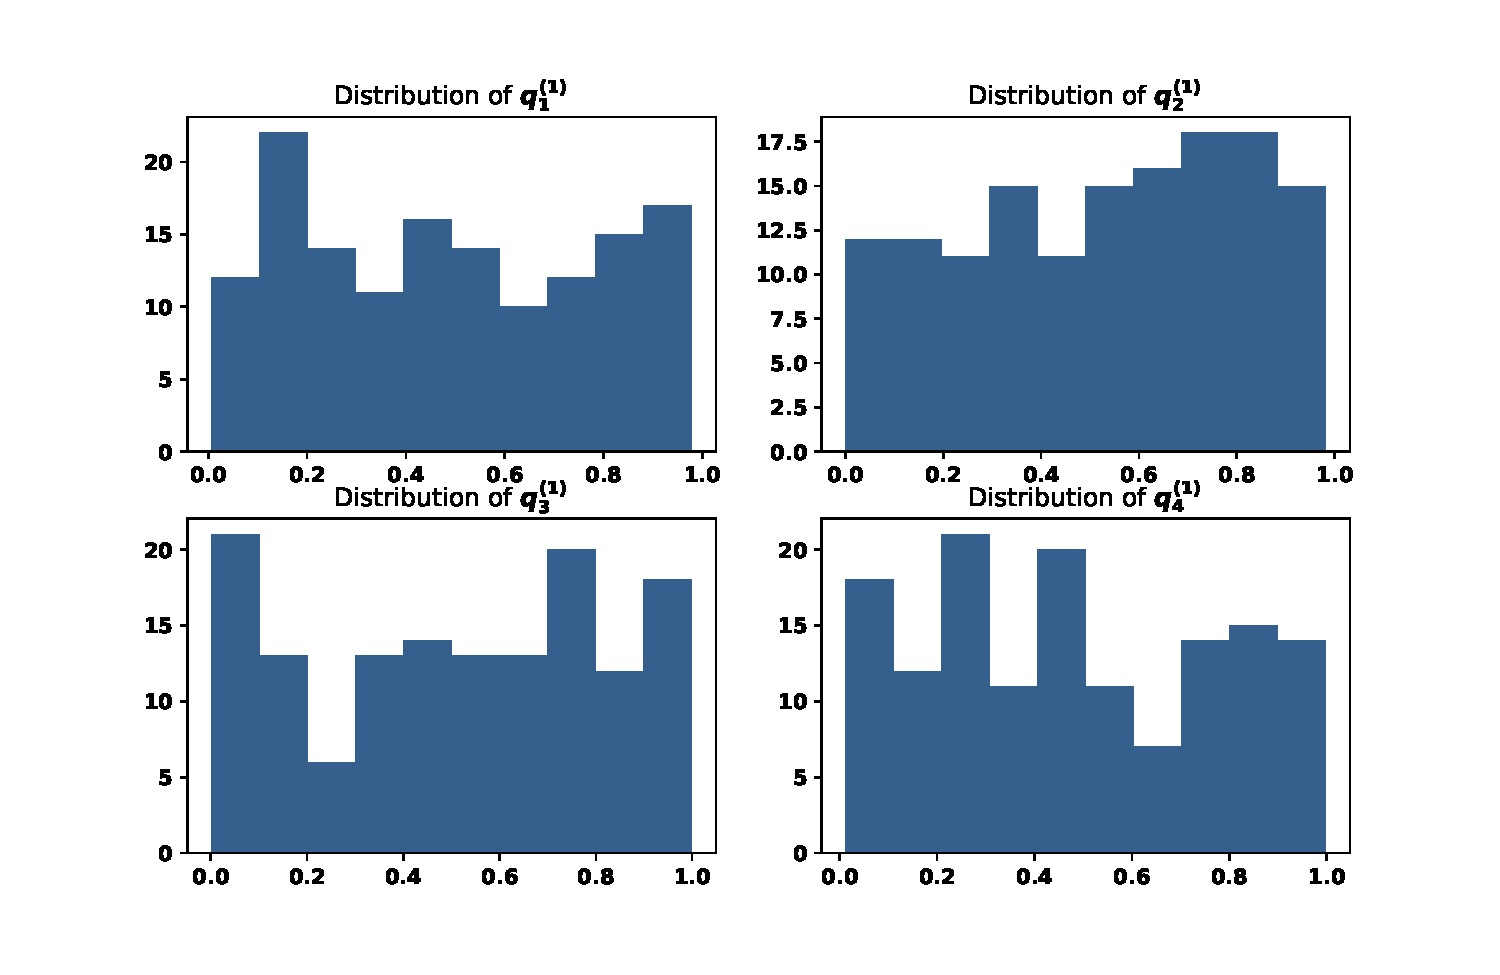
\includegraphics[width=\linewidth]{src/chapters/05/paper/Memory-size-in-the-prisoners-dilemma/img/first_opponent_probabilities_with_gambler.pdf}
        \subcaption{Distributions of first opponents' probabilities for longer memory experiment.}
        \label{fig:first_opponents_probabilities_with_gambler}
    \end{subfigure}
    \begin{subfigure}{0.49\textwidth}
        \centering
        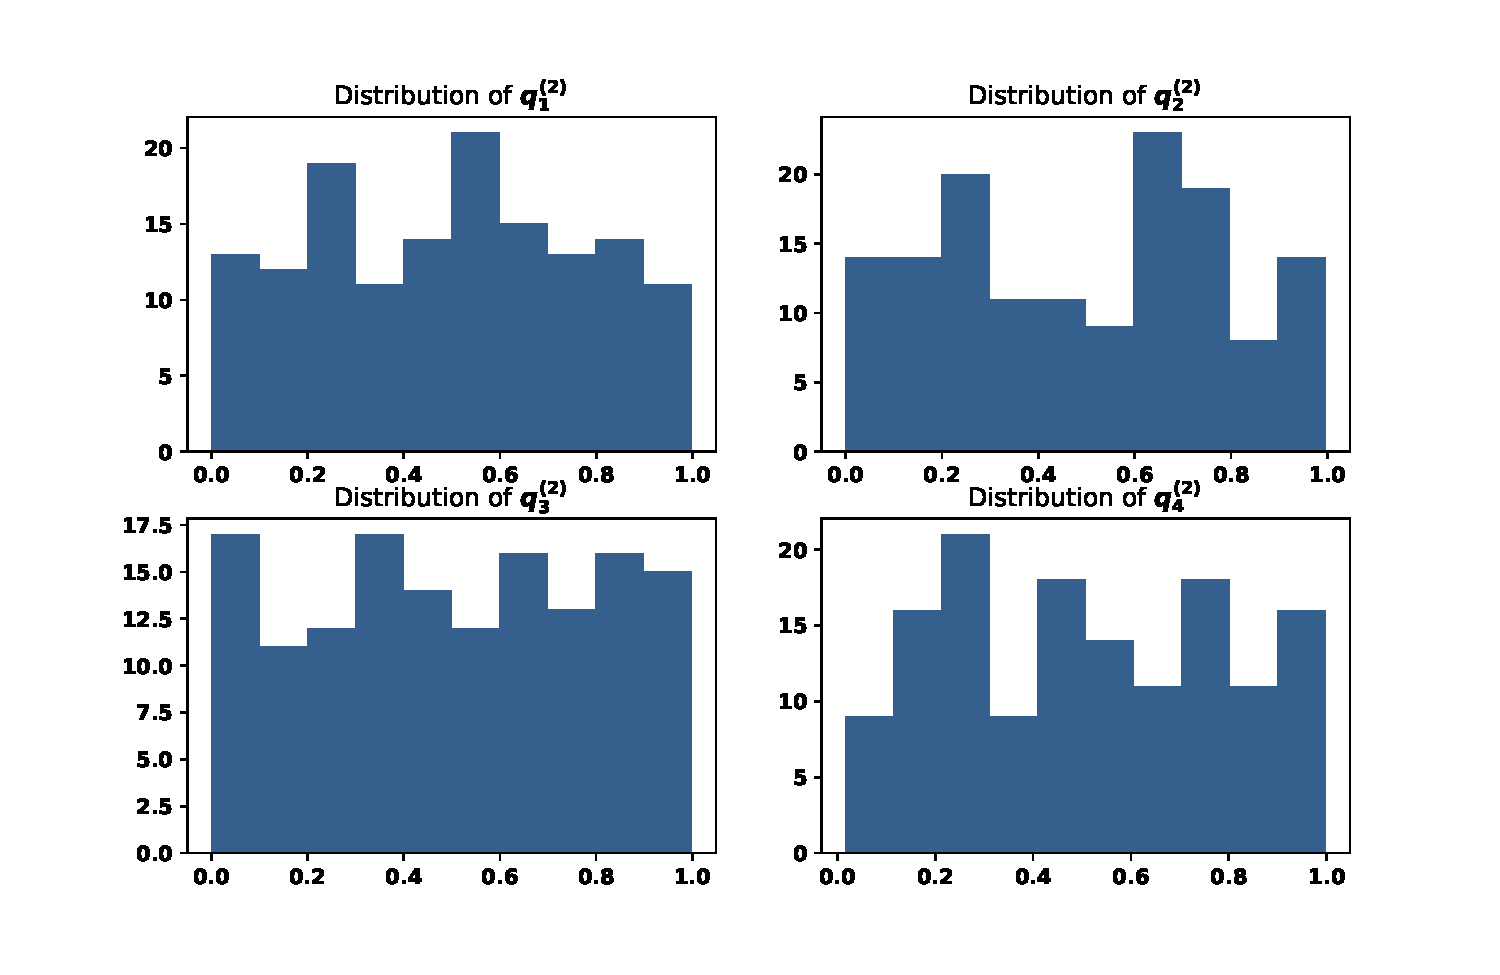
\includegraphics[width=\linewidth]{src/chapters/05/paper/Memory-size-in-the-prisoners-dilemma/img/second_opponent_probabilities_with_gambler.pdf}
        \subcaption{Distributions of second opponents' probabilities for longer memory experiment.}
        \label{fig:second_opponents_probabilities_with_gambler}
    \end{subfigure}
\end{figure}

The utilities of both strategies are plotted against each other in
Figure~\ref{fig:utilities_gambler_mem_one}. Although Gambler has an infinite
memory (in order to remember the opening moves of the opponent) the information
the strategy considers is not significantly larger than memory-one strategies.
Even so, it is evident from Figure~\ref{fig:utilities_gambler_mem_one} that
Gambler always performs as well as the best response memory-one or better. This seems to be at odd with the
result of~\cite{Press2012} that against a memory-one opponent having a longer memory
will not give a strategy any
advantage. However, against two memory-one opponents Gambler's performance is better than
the optimal memory-one strategy. This is evidence that in the case of two opponents having a
shorter memory is limiting.

\begin{figure}[!htbp]
    \centering
    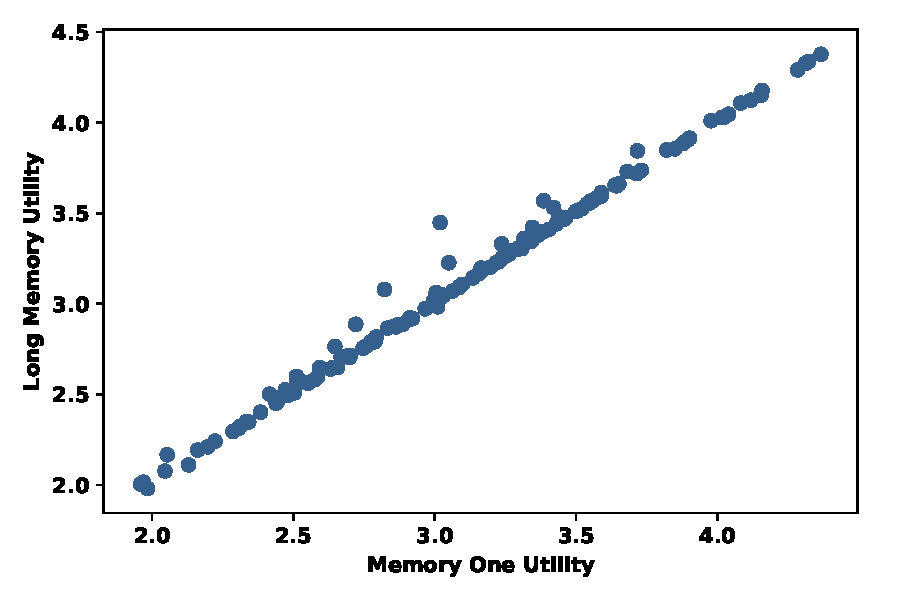
\includegraphics[width=.55\textwidth]{src/chapters/05/paper/Memory-size-in-the-prisoners-dilemma/img/gambler_performance_against_mem_one.pdf}
    \caption{Utilities of Gambler and best response memory-one strategies for
    130 different pair of opponents.}\label{fig:utilities_gambler_mem_one}
\end{figure}

\section{Conclusion}

This manuscript has considered \textit{best response} strategies in the IPD game, and
more specifically, \textit{memory-one best responses}. It has proven that there is
a compact way of identifying a memory-one best response to a group of opponents,
and moreover, that there exists a condition for which in an
environment of memory-one opponents defection is the stable choice.
The later parts of this paper focused on a series of empirical results, where it
was shown that the performance and the evolutionary stability of memory-one
strategies rely not on extortion but on adaptability. Finally, it was shown that
memory-one strategies' performance is limited by their memory in cases where
they interact with multiple opponents.

Following the work described in~\cite{Nowak1989}, where it was shown that the
utility between two memory-one strategies can be estimated by a Markov
stationary state, we proved that the utilities can be written as a ration of two
quadratic forms in $R^4$, Theorem~\ref{theorem:quadratic_form_u}. This was
extended to include multiple opponents, as the IPD is commonly studied in such
situations, Theorem~\ref{theorem:tournament_utility}.
The formulation of Theorem~\ref{theorem:tournament_utility} allowed us to introduce an approach for identifying
memory-one best responses to any number of opponents;
Lemma~\ref{lemma:memone_group_best_response}. This does not only have game
theoretic novelty, but also a mathematical novelty of solving quadratic ratio
optimisation problem where the quadratics are non concave. The results of
Lemma~\ref{lemma:memone_group_best_response} were also used to define a
condition for which defection is known to be stable.

This manuscript presented several experimental results. These results were mainly to
investigate the behaviour of memory-one strategies and their limitations. In
Sections~\ref{subsection:best_response_n_2}
and~\ref{subsection:best_respnse_evolutionary_setting}, a large data set which
contained best responses in tournaments and in evolutionary settings for $N=2$
was generated. This allowed us to investigate their respective behaviours, and
whether it was extortionate acts that made them the most favourable strategies.
However, it was shown that it was not extortion but adaptability that allowed
the strategies to gain the most from their interactions.
In evolutionary settings it was specifically shown that being adaptable and being
able to forgive after being tricked were key factors. In Section~\ref{subsection:longer_memory_best_response}, the performance of
memory-one strategies was put against the performance of a longer memory
strategy called Gambler. There were several cases where Gambler would outperform
the memory-one strategy, however, a memory-one strategy never managed to outperform
a Gambler. This result occurred whilst considering a Gambler with a sufficiently
larger memory but not a sufficiently larger amount of information regarding
the game.

All the empirical results presented in this manuscript have been for the
case of $N=2$. In future work we would consider larger values of $N$, however, we
believe that for larger values of $N$ the results that have been presented here would
only be more evident.

% \section{Acknowledgements}

% A variety of software libraries have been used in this work:

% \begin{itemize}
%     \item The Axelrod library for IPD simulations~\cite{axelrodproject}.
%     \item The Scikit-optimize library for an implementation of Bayesian optimisation~\cite{tim_head_2018_1207017}.
%     \item The Matplotlib library for visualisation~\cite{hunter2007matplotlib}.
%     \item The SymPy library for symbolic mathematics~\cite{sympy}.
%     \item The Numpy library for data manipulation~\cite{walt2011numpy}.
% \end{itemize}

% % Bibliography
% \bibliographystyle{plain}
% \bibliography{bibliography.bib}


\section{Proofs of the Theorems}\label{section:appendix_a}

% \subsection{Proof of Theorem~\ref{theorem:quadratic_form_u}}\label{appendix:proof_theorem_one}
% The utility of a memory one player \(p\) against an opponent \(q\),
\(u_q(p)\), can be written as a ratio of two quadratic forms on \(R^4\).

\begin{proof}

In Section~\ref{section:utility}, it was discussed that \(u_q(p)\) it's the product
of the steady states \(v\) and the PD payoffs,

\[u_q(p) = v \cdot (R, S, T, P).\]

More specifically, with \((R, P, S, T) = (3, 1, 0, 5)\)

\begingroup
\footnotesize
\begin{equation}
    u_q(p) =
    \left(
      \frac
        {\parbox{6in}{$
            p_{1} p_{2} (q_{1} q_{2} - 5 q_{1} q_{4} - q_{1} - q_{2} q_{3} + 5 q_{3} q_{4} + q_{3}) + p_{1} p_{3} (- q_{1} q_{3} + q_{2} q_{3}) + p_{1} p_{4} (5 q_{1} q_{3} - 5 q_{3} q_{4}) + p_{3} p_{4} (- 3 q_{2} q_{3} + 3 q_{3} q_{4}) +$ \\
            \hspace*{1cm} $ p_{2} p_{3} (- q_{1} q_{2} + q_{1} q_{3} + 3 q_{2} q_{4} + q_{2} - 3 q_{3} q_{4} - q_{3}) + p_{2} p_{4} (- 5 q_{1} q_{3} + 5 q_{1} q_{4} + 3 q_{2} q_{3} - 3 q_{2} q_{4} + 2 q_{3} - 2 q_{4}) + $ \\
            \hspace*{1cm} $ p_{1} (- q_{1} q_{2} + 5 q_{1} q_{4} + q_{1}) + p_{2} (q_{2} q_{3} - q_{2} - 5 q_{3} q_{4} - q_{3} + 5 q_{4} + 1) + p_{3} (q_{1} q_{2} - q_{2} q_{3} - 3 q_{2} q_{4} - q_{2} + q_{3}) +$ \\
            \hspace*{4cm} $ p_{4} (- 5 q_{1} q_{4} + 3 q_{2} q_{4} + 5 q_{3} q_{4} - 5 q_{3} + 2 q_{4}) + q_{2} - 5 q_{4} - 1$
        }}
        {\parbox{6in}{$
        p_{1} p_{2} (q_{1} q_{2} - q_{1} q_{4} - q_{1} - q_{2} q_{3} + q_{3} q_{4} + q_{3}) + p_{1} p_{3} (- q_{1} q_{3} + q_{1} q_{4} + q_{2} q_{3} - q_{2} q_{4}) + p_{1} p_{4} (- q_{1} q_{2} + q_{1} q_{3} + q_{1} + q_{2} q_{4} - q_{3} q_{4} - q_{4}) +$ \\
        $ p_{2} p_{3} (- q_{1} q_{2} + q_{1} q_{3} + q_{2} q_{4} + q_{2} - q_{3} q_{4} - q_{3}) + p_{2} p_{4} (- q_{1} q_{3} + q_{1} q_{4} + q_{2} q_{3} - q_{2} q_{4}) + p_{3} p_{4} (q_{1} q_{2} - q_{1} q_{4} - q_{2} q_{3} - q_{2} + q_{3} q_{4} + q_{4}) + $ \\
        $ p_{1} (- q_{1} q_{2} + q_{1} q_{4} + q_{1}) + p_{2} (q_{2} q_{3} - q_{2} - q_{3} q_{4} - q_{3} + q_{4} + 1) + p_{3} (q_{1} q_{2} - q_{2} q_{3} - q_{2} + q_{3} - q_{4}) + p_{4} (- q_{1} q_{4} + q_{2} + q_{3} q_{4} - q_{3} + q_{4} - 1) + $ \\
        \hspace*{7cm} $q_{2} - q_{4} - 1$
      }}
    \right).
\end{equation}
\endgroup

Let us consider the numerator of the \(u_q(p)\). The cross product terms \(p_ip_j\)
are given by,

\begingroup
\footnotesize
\begin{align*}
p_{1} p_{2} (q_{1} q_{2} - 5 q_{1} q_{4} - q_{1} - q_{2} q_{3} + 5 q_{3} q_{4}
+ q_{3}) + p_{1} p_{3} (- q_{1} q_{3} + q_{2} q_{3}) + p_{1} p_{4} (5 q_{1} q_{3} -
5 q_{3} q_{4}) + p_{3} p_{4} (- 3 q_{2} q_{3} + 3 q_{3} q_{4}) +  \\
p_{2} p_{3} (- q_{1} q_{2} + q_{1} q_{3} + 3 q_{2} q_{4} + q_{2} - 3 q_{3} q_{4} - q_{3}) +
p_{2} p_{4} (- 5 q_{1} q_{3} + 5 q_{1} q_{4} + 3 q_{2} q_{3} - 3 q_{2} q_{4} +
2 q_{3} - 2 q_{4}).
\end{align*}
\endgroup

This can be re written in a matrix format given by (\ref{eq:cross_product_coeffs}).

\begin{equation}\label{eq:cross_product_coeffs}
    \resizebox{0.8\linewidth}{!}{\arraycolsep=2.5pt%
    \boldmath\( 
    (p_1, p_2, p_3, p_4) \frac{1}{2} \left[\begin{matrix}0 & - \left(q_{1} - q_{3}\right) \left(q_{2} - 5 q_{4} - 1\right) & q_{3} \left(q_{1} - q_{2}\right) & - 5 q_{3} \left(q_{1} - q_{4}\right)\\- \left(q_{1} - q_{3}\right) \left(q_{2} - 5 q_{4} - 1\right) & 0 & \left(q_{2} - q_{3}\right) \left(q_{1} - 3 q_{4} - 1\right) & \left(q_{3} - q_{4}\right) \left(5 q_{1} - 3 q_{2} - 2\right)\\q_{3} \left(q_{1} - q_{2}\right) & \left(q_{2} - q_{3}\right) \left(q_{1} - 3 q_{4} - 1\right) & 0 & 3 q_{3} \left(q_{2} - q_{4}\right)\\- 5 q_{3} \left(q_{1} - q_{4}\right) & \left(q_{3} - q_{4}\right) \left(5 q_{1} - 3 q_{2} - 2\right) & 3 q_{3} \left(q_{2} - q_{4}\right) & 0\end{matrix}\right] \begin{pmatrix} 
    p_1 \\
    p_2 \\
    p_3 \\
    p_4 \end{pmatrix}
    \) }
\end{equation}

Similarly, the linear terms are given by,

\begingroup
\footnotesize
\begin{align*}
p_{1} (- q_{1} q_{2} + 5 q_{1} q_{4} + q_{1}) + p_{2} (q_{2} q_{3} - q_{2} - 5 q_{3} q_{4} - q_{3} + 5 q_{4} + 1) + p_{3} (q_{1} q_{2} - q_{2} q_{3} - 3 q_{2} q_{4} - q_{2} + q_{3}) + \\
p_{4} (- 5 q_{1} q_{4} + 3 q_{2} q_{4} + 5 q_{3} q_{4} - 5 q_{3} + 2 q_{4}).
\end{align*}
\endgroup

and the expression can be written using a matrix format as (\ref{eq:linear_coeffs}).

\begin{equation}\label{eq:linear_coeffs}
    \resizebox{0.38\linewidth}{!}{\arraycolsep=2.5pt%
    \boldmath\(
    (p_1, p_2, p_3, p_4) \left[\begin{matrix}q_{1} \left(q_{2} - 5 q_{4} - 1\right)\\- \left(q_{3} - 1\right) \left(q_{2} - 5 q_{4} - 1\right)\\- q_{1} q_{2} + q_{2} q_{3} + 3 q_{2} q_{4} + q_{2} - q_{3}\\5 q_{1} q_{4} - 3 q_{2} q_{4} - 5 q_{3} q_{4} + 5 q_{3} - 2 q_{4}\end{matrix}\right]\)}
\end{equation}

Finally, the constant term of the numerator, which is obtained by substituting
$p=(0, 0, 0, 0)$, is given by (\ref{eq:constant}).

\begin{equation}\label{eq:constant}
q_{2} - 5 q_{4} - 1
\end{equation}

Combining equations (\ref{eq:cross_product_coeffs}), (\ref{eq:linear_coeffs}) and (\ref{eq:constant})
gives that the numerator of \(u_q(p)\) can be written as,

\begingroup
\tiny\boldmath
\begin{align*}
    \frac{1}{2}p & \left[\begin{matrix}0 & - \left(q_{1} - q_{3}\right) \left(q_{2} - 5 q_{4} - 1\right) & q_{3} \left(q_{1} - q_{2}\right) & - 5 q_{3} \left(q_{1} - q_{4}\right)\\- \left(q_{1} - q_{3}\right) \left(q_{2} - 5 q_{4} - 1\right) & 0 & \left(q_{2} - q_{3}\right) \left(q_{1} - 3 q_{4} - 1\right) & \left(q_{3} - q_{4}\right) \left(5 q_{1} - 3 q_{2} - 2\right)\\q_{3} \left(q_{1} - q_{2}\right) & \left(q_{2} - q_{3}\right) \left(q_{1} - 3 q_{4} - 1\right) & 0 & 3 q_{3} \left(q_{2} - q_{4}\right)\\- 5 q_{3} \left(q_{1} - q_{4}\right) & \left(q_{3} - q_{4}\right) \left(5 q_{1} - 3 q_{2} - 2\right) & 3 q_{3} \left(q_{2} - q_{4}\right) & 0\end{matrix}\right] p^T +  \\
    & \left[\begin{matrix}0 & - \left(q_{1} - q_{3}\right) \left(q_{2} - 5 q_{4} - 1\right) & q_{3} \left(q_{1} - q_{2}\right) & - 5 q_{3} \left(q_{1} - q_{4}\right)\\- \left(q_{1} - q_{3}\right) \left(q_{2} - 5 q_{4} - 1\right) & 0 & \left(q_{2} - q_{3}\right) \left(q_{1} - 3 q_{4} - 1\right) & \left(q_{3} - q_{4}\right) \left(5 q_{1} - 3 q_{2} - 2\right)\\q_{3} \left(q_{1} - q_{2}\right) & \left(q_{2} - q_{3}\right) \left(q_{1} - 3 q_{4} - 1\right) & 0 & 3 q_{3} \left(q_{2} - q_{4}\right)\\- 5 q_{3} \left(q_{1} - q_{4}\right) & \left(q_{3} - q_{4}\right) \left(5 q_{1} - 3 q_{2} - 2\right) & 3 q_{3} \left(q_{2} - q_{4}\right) & 0\end{matrix}\right] p + q_{2} - 5 q_{4} - 1
\end{align*}
\endgroup

and equivalently as,

\[\frac{1}{2}pQp^T + cp + a\]

where \(Q\) \(\in \R^{4\times4}\) is a square matrix defined by the
transition probabilities of the opponent \(q_1, q_2, q_3, q_4\) as follows:

\begin{equation*}
    \resizebox{0.9\linewidth}{!}{\arraycolsep=2.5pt%
    \boldmath\(
    Q = \left[\begin{matrix}0 & - \left(q_{1} - q_{3}\right) \left(q_{2} - 5 q_{4} - 1\right) & q_{3} \left(q_{1} - q_{2}\right) & - 5 q_{3} \left(q_{1} - q_{4}\right)\\- \left(q_{1} - q_{3}\right) \left(q_{2} - 5 q_{4} - 1\right) & 0 & \left(q_{2} - q_{3}\right) \left(q_{1} - 3 q_{4} - 1\right) & \left(q_{3} - q_{4}\right) \left(5 q_{1} - 3 q_{2} - 2\right)\\q_{3} \left(q_{1} - q_{2}\right) & \left(q_{2} - q_{3}\right) \left(q_{1} - 3 q_{4} - 1\right) & 0 & 3 q_{3} \left(q_{2} - q_{4}\right)\\- 5 q_{3} \left(q_{1} - q_{4}\right) & \left(q_{3} - q_{4}\right) \left(5 q_{1} - 3 q_{2} - 2\right) & 3 q_{3} \left(q_{2} - q_{4}\right) & 0\end{matrix}\right]\)},
\end{equation*}

\(c\) \(\in \R^{4 \times 1}\) is similarly defined by:

\begin{equation*}
    \resizebox{0.3\linewidth}{!}{\arraycolsep=2.5pt%
    \boldmath\(c = \left[\begin{matrix}q_{1} \left(q_{2} - 5 q_{4} - 1\right)\\- \left(q_{3} - 1\right) \left(q_{2} - 5 q_{4} - 1\right)\\- q_{1} q_{2} + q_{2} q_{3} + 3 q_{2} q_{4} + q_{2} - q_{3}\\5 q_{1} q_{4} - 3 q_{2} q_{4} - 5 q_{3} q_{4} + 5 q_{3} - 2 q_{4}\end{matrix}\right]\),}
\end{equation*}

and \(a = - q_{2} + 5 q_{4} + 1\).

The same process is done for the denominator.
\end{proof}

% \subsection{Proof of Theorem~\ref{theorem:concavity}}\label{appendix:proof_theorem_three}
% The utility \(u_q(p)\) is non concave and neither are it's numerator or
denominator. Furthermore, the denominator is not always strictly positive.

\begin{proof}

The utility \(u_q(p)\) is non concave because the concavity condition fails for at
least one pair of points see Appendix~\ref{appendix:non_concave}.

Furthermore, regarding the numerator and denominator of \(u_q(p)\)
in~\cite{Anton2014} it is stated that a quadratic form will be concave if and
only if it's symmetric matrix is semi-negative definite. A matrix \(A\) is
semi-negative definite if:

\begin{equation}\label{def:semi_negative}
|A|_i \leq 0 \text{ for } i \text{ is odd and } |A|_i \geq 0  \text{ for } i
\text{ is even,}
\end{equation}

where \(|A|_i\) is the eigenvalues of the submatrix \(A_i\).

For (\ref{eq:optimisation_quadratic}), neither \(\frac{1}{2}pQp^T + cp + a\)
or \(\frac{1}{2}p\bar{Q}p^T + \bar{c}p + \bar{a}\) are concave because for an even \(i=2\):

\[|Q|_2 = - \left(q_{1} - q_{3}\right)^{2} \left(q_{2} - 5 q_{4} - 1\right)^{2} \text{and}\]
\[|\bar{Q}|_2 =- \left(q_{1} - q_{3}\right)^{2} \left(q_{2} - q_{4} - 1\right)^{2}\]

are negative.

Moreover, for a quadratic to be strictly positive it has to be positive definite.
A quadratic form is positive definite iff every eigenvalue of is positive,
however, \(\frac{1}{2}p\bar{Q}p^T + \bar{c}p + \bar{a}\) is not positive definite
because:

\[|\bar{Q}|_2 =- \left(q_{1} - q_{3}\right)^{2} \left(q_{2} - q_{4} - 1\right)^{2}\]

is negative.
\end{proof}

% \subsection{Proof of Lemma~\ref{lemma:memone_group_best_response}}\label{appendix:proof_lemma_four}
% \begin{proof}
The optimal behaviour of a memory-one strategy player
\(p^* \in \R_{[0, 1]} ^ 4\)
against a set of \(N\) opponents \(\{q^{(1)}, q^{(2)}, \dots, q^{(N)} \}\)
for \(q^{(i)} \in \R_{[0, 1]} ^ 4\) is established by:

\[p^* = \textnormal{argmax}\left(\sum\limits_{i=1} ^ N  u_q(p)\right), \ p \in S_q,\]

where \(S_q\) is given by (\ref{eq:s_q_set}).

The optimisation problem of (\ref{eq:mo_tournament_optimisation}) can be
written as:

\begin{equation}\label{eq:mo_tournament_optimisation_standard}
    \begin{aligned}
    \max_p: & \ \sum_{i=1} ^ {N} {u_q}^{(i)} (p)
    \\
    \text{such that}: p_i & \leq 1 \text{ for } \in \{1, 2, 3, 4\} \\
    - p_i & \leq 0 \text{ for } \in \{1, 2, 3, 4\} \\
    \end{aligned}
\end{equation}

The optimisation problem has two inequality constraints and regarding the optimality
this means that:

\begin{itemize}
    \item either the optimum is away from the boundary of the optimization domain, and so the constraints plays no role;
    \item or the optimum is on the constraint boundary.
\end{itemize}

Thus, the following three cases must be considered:

\textbf{Case 1:} The solution is on the boundary and any of the possible
combinations for $p_i \in \{0, 1\}$ for $i \in \{1, 2, 3, 4\}$ are candidate
optimal solutions.

\textbf{Case 2:} The optimum is away from the boundary of the optimization domain
and the interior solution $p^*$ necessarily satisfies the condition
\(\frac{d}{dp} \sum\limits_{i=1} ^ N  u_q(p^*) = 0\).

\textbf{Case 3:} The optimum is away from the boundary of the optimization domain
but some constraints are equalities. The candidate solutions in this case
are any combinations of $p_j \in \{0, 1\} \quad \text{and} \quad \frac{d}{dp_k} 
\sum\limits_{i=1} ^ N  u_q^{(i)}(p) = 0$ 
forall $ j \in J \text{ \& } k \in K \text{ forall } J, K
\text{ where } J \cap K = \O \text{ and } J \cup K = \{1, 2, 3, 4\}.$

Combining cases 1-3 a set of candidate solution is constructed as:

\begin{equation*}
    S_q =
    \left\{p \in \mathbb{R} ^ 4 \left|
        \begin{aligned}
            \bullet\quad p_j \in \{0, 1\} & \quad \text{and} \quad \frac{d}{dp_k} 
            \sum\limits_{i=1} ^ N  u_q^{(i)}(p) = 0
            \quad \text{for all} \quad j \in J \quad \&  \quad k \in K  \quad \text{for all} \quad J, K \\
            & \quad \text{where} \quad J \cap K = \O \quad
            \text{and} \quad J \cup K = \{1, 2, 3, 4\}.\\
            \bullet\quad  p \in \{0, 1\} ^ 4
        \end{aligned}\right.
    \right\}.
\end{equation*}

This set is denoted as $S_q$ and the optimal solution to
(\ref{eq:mo_tournament_optimisation}) is the point from $S_q$ for which the
utility is maximised.

% The Lagrangian\cite{bertsekas2014} of (\ref{eq:mo_tournament_optimisation_standard})
% is then given by,

% \begin{align}
% L(p_1, p_2, p_3, p_4, \lambda_1, \lambda_2, \dots, \lambda_8) = \sum\limits_{i=1} ^ N  u_q(p)
% + \lambda_1 (p_1 - 1) + \lambda_2 (p_2 - 1) + \lambda_3 (p_3 - 1) + \lambda_4 (p_4 - 1) + \\
% \lambda_5( - p_1) + \lambda_6 (- p_2) + \lambda_7 (- p_3) + \lambda_8 (- p_4)
% \end{align}

% This gives the following Karush-Kuhn-Tucker~\cite{Giorgi2016} conditions:

% \begin{align}
% \frac{d\sum\limits_{i=1} ^ N  u_q(p)}{dp_1} + \lambda_1 -\lambda_5 = 0 \\
% \frac{d\sum\limits_{i=1} ^ N  u_q(p)}{dp_2} + \lambda_2 -\lambda_6 = 0 \\
% \frac{d\sum\limits_{i=1} ^ N  u_q(p)}{dp_3} + \lambda_3 -\lambda_7 = 0 \\
% \frac{d\sum\limits_{i=1} ^ N  u_q(p)}{dp_4} + \lambda_4 -\lambda_8 = 0 \\
% \lambda_i (p_i - 1) = 0 \text{ for } i \in \{1, 2, 3, 4\} \\
% -\lambda_5 p_1 = 0 \\
% -\lambda_6 p_2 = 0 \\
% -\lambda_7 p_3 = 0 \\
% -\lambda_8 p_4 = 0
%     \end{align}

% There are eight complementarity conditions (37) - (41), thus a total of 16 cases
% to be checked.

% \textbf{Case 1:} \(\lambda_1 = \lambda_2 = \dots = \lambda_8 = 0\). The best response
% is given by the roots of the partial derivatives
% \(\frac{d\sum\limits_{i=1} ^ N  u_q(p)}{dp} = 0\).

% \textbf{Case 2:} \(\lambda_1 = \lambda_2 = \lambda_3 = \lambda_4 = 0\) and
% \(\lambda_5 \neq 0, \lambda_6 \neq 0,  \lambda_7 \neq 0, \lambda_8 \neq 0\). The
% best response is given by \(p_1 = p_2 = p_3 = p_4 = 0\).

% \textbf{Case 3:} \(\lambda_5 = \lambda_6 = \lambda_7 = \lambda_8 = 0\) and
% \(\lambda_1 \neq 0, \lambda_2 \neq 3,  \lambda_4 \neq 0, \lambda_5 \neq 0\). The
% best response is given by \(p_1 = p_2 = p_3 = p_4 = 1\).


\end{proof}

% \section{Further Examples}\label{section:appendix_b}

% \subsection{Example of non concavity for \(u(p)\) }\label{appendix:non_concave}
% A function \(f(x)\) is concave on an interval \([a, b]\) if, for any two
points \(x_1, x_2 \in [a, b]\) and any \(\lambda \in [0, 1]\), 

\begin{equation}\label{eq:concave}
f (\lambda x_1 + (1 - \lambda )x_2 ) \geq \lambda f (x_1 ) + (1 - \lambda )f (x_2 ).
\end{equation}

Let \(f\) be \(u_{(\frac{1}{3}, \frac{1}{3}, \frac{1}{3}, \frac{1}{3})}\).
For \(x_1 = (\frac{1}{4}, \frac{1}{2}, \frac{1}{5} , \frac{1}{2}),
x_2 = (\frac{8}{10}, \frac{1}{2}, \frac{9}{10} , \frac{7}{10})\) and
\(\lambda=0.1\), direct substitution in (\ref{eq:concave}) gives:

\scalebox{0.85}{\parbox{\linewidth}{%
\begin{align*}
    u_{(\frac{1}{3}, \frac{1}{3}, \frac{1}{3}, \frac{1}{3})}
    \left( 0.1 \left(\frac{1}{4}, \frac{1}{2}, \frac{1}{5} , \frac{1}{2}\right)
    + 0.9 \left(\frac{8}{10}, \frac{1}{2}, \frac{9}{10} , \frac{7}{10}\right) \right) & \geq
    0.1 \times u_{(\frac{1}{3}, \frac{1}{3}, \frac{1}{3}, \frac{1}{3})}
    \left(\left(\frac{1}{4}, \frac{1}{2}, \frac{1}{5} , \frac{1}{2}\right) \right) 
    + 0.9 \times u_{(\frac{1}{3}, \frac{1}{3}, \frac{1}{3}, \frac{1}{3})}
    \left(\left(\frac{8}{10}, \frac{1}{2}, \frac{9}{10} , \frac{7}{10}\right) \right) \Rightarrow\\
    1.485 & \geq 0.1 \times 1.790 + 0.9 \times 1.457 \Rightarrow \\
    1.485 & \geq 1.490
\end{align*}
}}

which can not hold. Thus \(u_{(\frac{1}{3}, \frac{1}{3}, \frac{1}{3}, \frac{1}{3})}\)
is not concave.
% \chapter{Best Response Sequences in the Iterated Prisoner's Dilemma}\label{chapter:best_response_sequence}

\begin{center}
    The research reported in this Chapter has been carried out with:

    Axerod-Python library version: 4.2.0 \\
    Associated data set: \cite{Glynatsi2020_sequences} \\ \vspace{.5cm}
\end{center}

\section{Introduction}

In this Chapter best response strategies are explored in the form
of static sequences of moves, in order to generate a large data set of best
response sequences to a collection of opponents.

The data set is generated by considering best response sequences in finite IPD
matches of 205 turns against \numberofstrategiesbestsequences strategies
available in the APL. These best response sequences are not obtained explicitly
but instead are estimated heuristically using a genetic algorithm devised for
this purpose.

The purpose of a large collection of best response sequences is
to serve as training data in Chapter~\ref{chapter:lstm} which aims to train a
recurrent neural network as an IPD strategy. In Chapter~\ref{chapter:lstm} the
usage of the bespoke data set, which has been archived and made publicly
available~\cite{Glynatsi2020_sequences}, is discussed in more details. This
Chapter is structured as follow:

\begin{itemize}
    \item section~\ref{section:ipd_as_sequences} formalises the use of sequences to express a player in a
    finite IPD match.
    \item section~\ref{section:genetic_algorithm} describes the genetic algorithm
    used to estimate best response
    sequences.
    \item section~\ref{section:generating_sequences} details the process of
    generating best response sequences to a collection of
    \numberofstrategiesbestsequences strategies.
\end{itemize}

\section{Iterated Prisoner Dilemma Strategies as Sequences}\label{section:ipd_as_sequences}

In a finite \(N\) round IPD match a player that does not react to their opponent
can be defined by a sequence,

\begin{equation}
    S \in \{C, D\} ^ n, \text{where } 1 \leq n \leq N.
\end{equation}

Strategies that base their actions on sequences are already established in the
literature~\cite{Beaufils1997}, such as Periodic Player \(CD\), Periodic Player \(DC\),
Periodic Player \(CCD\) and Periodic Player \(DDC\)~\cite{Li2011, Mittal2009},
or as referred to in~\cite{Knight2016} Cycler \(CD\), Cycler \(DC\),
Cycler \(CCD\) and Cycler \(DDC\). These are strategies that play a given sequences
periodically, however, the strategies concerned with here play a given
sequence only once, thus \(n = N\).

As an example consider a match of 10 turns between the strategy \(S = \{D, D, D,
C, C, C, D, D, C, C\}\) and Cooperator. The match between the two strategies
is captured by Table~\ref{table:s_vs_cooperator} where \(U(s_1, s_2)\in
\mathbb{R}^2\) is the average score per turn scored by strategies \(s_1\) and
\(s_2\).

\begin{table}[htb]
\centering
\begin{tabular}{cccccccccccc}
    & \textbf{1} & \textbf{2} & \textbf{3} & \textbf{4}  & \textbf{5} & \textbf{6} & \textbf{7} & \textbf{8}  & \textbf{9} & \textbf{10} & 
    \(U(S, \text{Cooperator})\) \\ \midrule
    \(S\) & \(D\) & \(D\) & \(D\) & \(C\) & \(C\) & \(C\) & \(D\) & \(D\) & \(C\) & \(C\) & 4.0 \\
    Cooperator & \(C\) & \(C\) & \(C\) & \(C\) & \(C\) & \(C\) & \(C\) & \(C\) & \(C\) & \(C\) & 1.5 \\ \bottomrule
\end{tabular}
\caption{The interactions of a 10 turns match between \(S = \{D, D, D, C, C, C, D, D, C, C\}\) and
Cooperator as well as the average score per turn achieved by each strategy.}\label{table:s_vs_cooperator}
\end{table}

A sequence strategy \(S\) can play against strategies that react to the history,
for example against Tit Tor Tat as demonstrated by Table~\ref{table:s_vs_tft},

\begin{table}[htb]
\centering
\begin{tabular}{cccccccccccc}
    & \textbf{1} & \textbf{2} & \textbf{3} & \textbf{4}  & \textbf{5} & \textbf{6} & \textbf{7} & \textbf{8}  & \textbf{9} & \textbf{10} &
    \(U(S, \text{Tit For Tat})\) \\ \midrule
    \(S\) & \(D\) & \(D\) & \(D\) & \(C\) & \(C\) & \(C\) & \(D\) & \(D\) & \(C\) & \(C\) & 2.2 \\
    Tit For Tat & \(C\) & \(D\) & \(D\) & \(D\) & \(C\) & \(C\) & \(C\) & \(D\) & \(D\) & \(C\) & 2.2 \\ \bottomrule
\end{tabular}
\caption{The interactions and average score per turn of a 10 turns match between
\(S = \{D, D, D, C, C, C, D, D, C, C\}\) and Tit For Tat.}\label{table:s_vs_tft}
\end{table}

and against stochastic strategies such as Random. Random cooperates with a
probability of \(0.5\) at each turn, and thus the actions of the strategy are
not deterministic. Random is a strategy that does react to the history, however,
the actions of stochastic strategies that react to the
history also differ between repetitions even when the history of the match is
the same. Tables~\ref{table:s_vs_random} and~\ref{table:s_vs_random_2} both
capture a match between \(S\) and a Random player. For a match of 10 turns
Random has a total of \(2^{10}\) possible plays.
In order to capture several different plays of stochastic strategies computer
seeding, further details of this are given in section~\ref{section:generating_sequences}.

\begin{table}[htb]
\centering
\begin{tabular}{cccccccccccc}
    & \textbf{1} & \textbf{2} & \textbf{3} & \textbf{4}  & \textbf{5} & \textbf{6} & \textbf{7} & \textbf{8}  & \textbf{9} & \textbf{10} &
    \(U(S, \text{Random})\) \\ \midrule
    \(S\) & \(D\) & \(D\) & \(D\) & \(C\) & \(C\) & \(C\) & \(D\) & \(D\) & \(C\) & \(C\) & 2.2 \\
    Random & \(D\) & \(D\) & \(C\) & \(C\) & \(D\) & \(C\) & \(D\) & \(C\) & \(C\) & \(D\) & 2.2 \\ \bottomrule
\end{tabular}
\caption{The interactions and average score per turn of a 10 turns match between
\(S = \{D, D, D, C, C, C, D, D, C, C\}\) and Random.}\label{table:s_vs_random}
\end{table}

\begin{table}[htb]
\centering
\begin{tabular}{cccccccccccc}
    & \textbf{1} & \textbf{2} & \textbf{3} & \textbf{4}  & \textbf{5} & \textbf{6} & \textbf{7} & \textbf{8}  & \textbf{9} & \textbf{10} & \(U(S, \text{Random})\) \\ 
    \midrule 
    \(S\) & \(D\) & \(D\) & \(D\) & \(C\) & \(C\) & \(C\) & \(D\) & \(D\) & \(C\) & \(C\) & 2.4 \\
    Random & \(C\) & \(D\) & \(D\) & \(C\) & \(C\) & \(C\) & \(D\) & \(D\) & \(C\) & \(C\) & 1.9 \\ \bottomrule
\end{tabular}
\caption{The interactions and average score per turn of a 10 turns match between
\(S = \{D, D, D, C, C, C, D, D, C, C\}\) and Random. The actions make by Random
are different to that of Table~\ref{table:s_vs_random}.}\label{table:s_vs_random_2}
\end{table}

As discussed in Chapters~\ref{chapter:introduction} and~\ref{chapter:memory_one},
a best response strategy is a strategy that achieves that most favourable outcome.
Thus a best response sequence against a given opponent \(Q\) corresponds
to a sequence \(S^*\) for which the average score per turn is maximised,
as given in~(\ref{eq:best_response_sequence}).

\begin{equation}\label{eq:best_response_sequence}
    \begin{aligned}
    \max_{S^*}: & U(S^*, Q)
    \end{aligned}
\end{equation}

Identifying best responses to some opponents can be a trivial problem. The
optimal sequence against a Cooperator is in an all \(D\) sequence. In fact the
sequence \(\{\underbrace{D, \dots, D}_{N}\}\) is a best response
against any sequence player whose plays are independent of the history.
However,
for some strategies identifying best responses is a complex problem.

Additionally, there are strategies that have multiple best response sequences. For
instance the strategy Adaptive introduced in~\cite{Li2011}. Adaptive opens by
playing a sequence of \(\{\underbrace{C, \dots, C}_{6}\}\) followed by a
sequence of \(\{\underbrace{D, \dots, D}_{5}\}\). The strategy then proceeds to
play either \(C\) or \(D\) depending on which action had a higher total score
for the strategy (the total score is recalculated at each turn). A sequence
maximises its average score against Adaptive by locking the strategy into
unconditional cooperations following its opening 11 turns sequence while the sequence
defects. In order
for cooperation to be the most favourable action for Adaptive the strategy needs to achieve
two mutual cooperations at its opening sequence. That is because the score achieved
by cooperating \(2 \times 3 + 4 \times 0 = 6\) is greater than the
score achieved by defecting \(1 \times 5 = 5\).
Any sequence which incorporates two cooperations in the first 6 turns
and defects thereafter is a best response sequence to Adaptive. Thus, there
can be \(2^{6}\) best response sequences to the strategy, for example \(S_{1}^*\) and \(S_{2}^*\),

\[S_{1}^* = \{C, D, D, D, D, C, D, D, D, D, D, D, D, D, D\}\]

\[S_{2}^* = \{D, D, C, C, D, D, D, D, D, D, D, D, D, D, D\}\]

where \(U(S_{1}^*, \text{Adaptive}) = U(S_{2}^*, \text{Adaptive}) = 3.4\).

Due to identifying best response sequences to some opponents being a complex
problem, and moreover, multiple best response sequences existing for some
opponents the best response sequences are not manually identified. Instead a
genetic algorithm is used to estimate them. A background on genetic algorithms
as well as the details of the specific genetic algorithm devised for this Chapter
are presented in the following section.

\section{Genetic Algorithm}\label{section:genetic_algorithm}

A genetic algorithm (GA) is a heuristic inspired by the process of natural
selection that belongs to the larger class of evolutionary algorithms. As stated
in~\cite{Whitley1994} GAs encode a potential solution to a
specific problem on a simple chromosome-like data structure, and apply
recombination operators to these structures in such a way as to preserve
critical information. GAs are often viewed as function
optimisers, although the range of problems to which they have been
applied is quite broad~\cite{Hou1994, Jones1997, Yang1998}.

An implementation of a GA begins with a \textit{population} \(P\) of
potential solutions, a number of \textit{generations} \(G \in \N\) and a cut-off or
\textit{bottleneck} \(b < |P|\). At each generation the algorithm scores and potentially
removes each member of the population \(p_i \in P\). This is done by using a
mapping from a member of the population to an ordered set based on an evaluation
function \(f\), usually \(f(p_i) \to \R\), and by only keeping the top \(b\)
ranking members (or proportion of members) by score at the end of each
generation. The rest of the member are discarded. By keeping the top ranked
individuals critical information regarding the successful candidates is
preserved and the population rebuilds on it by using a series of
\textit{crossovers} and \textit{mutations}.

\begin{itemize}
    \item During a crossover 2 members of the population are selected, and a new
    member is created based on combination of their ``genes''. The 2 selected members
    are commonly referred to as parents.
    \item Mutation is a probabilistic change that occurs to an individual,
    Mutation is commonly associated with a probability, denoted as \(p_m\).
    \(p_m\) is the probability of a mutation happening, either to the individual
    or to each gene of the individual.
\end{itemize}

A diagrammatical representation of a generic GA is given in Figure~\ref{fig:ga_flow_diagram}.

\begin{figure}[!htbp]
    \centering
    \includestandalone[width=.77\textwidth]{src/chapters/06/tex/ga_flow_diagram}
    \caption{Generic flow diagram of a GA.}\label{fig:ga_flow_diagram}
\end{figure}

The purpose of a GA here is to estimate a best response sequence to
a given opponent \(Q\). Consequently, the members of the population correspond to
sequences,

\[S_i \in P \text{ where } |S_i| = N\]

and the evaluation function corresponds to the
average score per turn of a sequence against \(Q\),

\[U(S_i, Q) \to \R \text{ for } S_i \in P.\]

More specifically, the exact GA used in this Chapter is given
by Algorithm~\ref{algorithm:genetic_algorithm}.

\begin{algorithm}[!htbp]
    \SetAlgoLined
    \KwIn{\(Q, N, b, p_m, G, K\)}
    \KwOut{The populations at each generation and the members' scores}
     \Begin{
     create initial population (Algorithm~\ref{algorithm:initial_population}) of members \(S\), where \(|S| = N\) and \(|P| = K\)\\
     \While{\(g_{i} < G\)}{
        score each member based on \(U(S_i, Q)\) for \(S_i \in P\) \\
        sort population based on scores \\
        keep \(b\) top members \\
        \While{\(|P|\) \(< K\)}{
            select 2 random members \\
            use members to create new member through crossover\\
            \For{gene in new member}{
            mutate gene with probability \(p_m\)}
            add new member to population\\
            }
     }}
     \caption{GA for estimating best response sequences to a given opponent \(Q\).}\label{algorithm:genetic_algorithm}
\end{algorithm}

The initial population is created using Algorithm~\ref{algorithm:initial_population}.

\begin{algorithm}[!htbp]
    \SetAlgoLined
    \KwIn{\(K, N\)}
    \KwOut{A population of size \(K\).}

    \Begin{
    set of cuts $\gets$ \(K\) evenly spaced numbers over \([1, N]\) \\
    \For{\(c \in\) set of cuts}{
        first new member $\gets$  \(\{\underbrace{C, \dots, C}_{c}, \underbrace{D, \dots, D}_{N-c}\}\) \\
        second new member $\gets$ \(\{\underbrace{D, \dots, D}_{c}, \underbrace{C, \dots, C}_{N-c}\}\) \\
        add both members to population
    }
        }
 \caption{Create initial population of individuals \(S\)}\label{algorithm:initial_population}
\end{algorithm}

Using a starting population of random guesses is a generally common approach in
the GA literature~\cite{Hou1994}. However, there is efficiency in using non
random starting populations~\cite{Drezner2005, Osaba2014}.
As discussed in section~\ref{section:ipd_as_sequences} the best response sequence
to any strategy that does not react to the history is a Defector. Moreover,
the best response sequence to several strategies include sequences mainly dominated
by cooperation expect in the last turns. These are
sequences that have been incorporated in the initial population. More specifically,
Algorithm~\ref{algorithm:initial_population} consider all the possible combinations
of:

\[\bullet \{\underbrace{C, \dots, C}_{c}, \underbrace{D, \dots, D}_{N-c}\} \text{ for } c \in \text{evenly spaced numbers over } [1, N] \text{ and}\]
\[\bullet \{\underbrace{D, \dots, D}_{c}, \underbrace{C, \dots, C}_{N-c}\} \text{ for } c \in \text{evenly spaced numbers over } [1, N].\]

The GA of Algorithm~\ref{algorithm:genetic_algorithm} has been implemented in the programming language Python
and it has been organised into a open source package called
\mintinline{python}{sequence_sensei} available at. %TODO archive
The properties of creating an initial population, crossover and mutation have been
implemented as individual functions.
The implementation of Algorithm~\ref{algorithm:initial_population} in the package
is given by Figure~\ref{fig:get_initial_population}.

\begin{figure}[!htbp]
\begin{sourcepy}
import numpy as np
def get_initial_population(half_size_of_population, sequence_length):
    """
    Generates an initial population of sequences. Note that the length
    of the population which is being generated is 2 * half_size_of_population.
    """
    cuts = np.linspace(1, sequence_length, half_size_of_population, dtype=int)
    sequences = []
    for cut in cuts:
        sequences.append(
            [1 for _ in range(cut)] + [0 for _ in range(sequence_length - cut)]
        )
        sequences.append(
            [0 for _ in range(cut)] + [1 for _ in range(sequence_length - cut)]
        )

    return sequences
\end{sourcepy}
\caption{Source code for the function \mintinline{python}{get_initial_population}
implemented in \mintinline{python}{sequence_sensei} which is used to create an
initial population of a given size.}\label{fig:get_initial_population}
\end{figure}

Figure~\ref{fig:get_initial_population_example} gives an example of creating an
initial population using the package. Note that the sequences are of 0s and 1s
and not IPD actions. The APL project can map binary number to actions such that
\(0 \to D\) and \(1 \to C\). This is also demonstrated in
Figure~\ref{fig:get_initial_population_example}.

\begin{figure}[!htbp]
    \begin{usagepy}
>>> import sequence_sensei as ss
>>> import numpy as np

>>> initial_population = ss.get_initial_population(
...     half_size_of_population=5, sequence_length=8
... )
>>> np.matrix(initial_population)
matrix([[1, 0, 0, 0, 0, 0, 0, 0],
        [0, 1, 1, 1, 1, 1, 1, 1],
        [1, 1, 0, 0, 0, 0, 0, 0],
        [0, 0, 1, 1, 1, 1, 1, 1],
        [1, 1, 1, 1, 0, 0, 0, 0],
        [0, 0, 0, 0, 1, 1, 1, 1],
        [1, 1, 1, 1, 1, 1, 0, 0],
        [0, 0, 0, 0, 0, 0, 1, 1],
        [1, 1, 1, 1, 1, 1, 1, 1],
        [0, 0, 0, 0, 0, 0, 0, 0]])

>>> import axelrod as axl
>>> np.matrix([[axl.Action(gene) for gene in member] for member in initial_population])
matrix([[C, D, D, D, D, D, D, D],
        [D, C, C, C, C, C, C, C],
        [C, C, D, D, D, D, D, D],
        [D, D, C, C, C, C, C, C],
        [C, C, C, C, D, D, D, D],
        [D, D, D, D, C, C, C, C],
        [C, C, C, C, C, C, D, D],
        [D, D, D, D, D, D, C, C],
        [C, C, C, C, C, C, C, C],
        [D, D, D, D, D, D, D, D]], dtype=object)

\end{usagepy}
\caption{Example of using \mintinline{python}{get_initial_population} to
generate a population of \(s=10\) and \(N=8\).}\label{fig:get_initial_population_example}
\end{figure}

In the GA, as given by Algorithm~\ref{algorithm:genetic_algorithm}, the
crossover occurs by randomly selecting two member of the population, while \(|P|
< K\), and randomly selecting a crossover point. Note that the crossover
point is smaller than \(N\). The new member initially inherits the
genes to the left of the crossover point of the first parent, and to the right
of the crossover point of the second parent.

For instance, given two member of the population \(S_1 = \{C, C, C, C, C, C, C, C, C, C\}\)
and \(S_2 = \{C, D, C, D, C, D, C, D, C, D\}\) and given that the crossover point is
4, this gives a new member \(S_3\):

\[S_3 = \{\underbrace{C, C, C, C}_{\text{from } S_1}, \underbrace{C, D, C, D, C, D}_{\text{from } S_2}\}.\]

The implementation of crossover in \mintinline{python}{sequence_sensei} is given
by Figure~\ref{fig:crossover_implementation}, and Figure~\ref{fig:crossover_usage}
demonstrates the usage of the \mintinline{python}{crossover} function to crossover
\(S_1\) and \(S_2\).

\begin{figure}[!htbp]
\begin{sourcepy}
import random

def crossover(sequence_one, sequence_two):
    sequence_length = len(sequence_one)
    crossover_point = random.randint(0, sequence_length)

    return sequence_one[:crossover_point] + sequence_two[crossover_point:]

\end{sourcepy}
\caption{Source code of the \mintinline{python}{crossover} function.}\label{fig:crossover_implementation}
\end{figure}

\begin{figure}[!htbp]
    \begin{usagepy}
>>> import random
>>> import sequence_sensei as ss

>>> turns = 10
>>> s_one = [1 for _ in range(turns)]
>>> s_two = [i % 2 for i in range(turns)]

>>> random.seed(0)
>>> new_member = ss.crossover(s_one, s_two)
>>> new_member
[1, 1, 1, 1, 1, 1, 0, 1, 0, 1]

\end{usagepy}
\caption{An example of using \mintinline{python}{crossover} function to crossover \(S_1\) and \(S_2\)}\label{fig:crossover_usage}
\end{figure}

Following the crossover between two members, a mutation is applied to new member
before it is added to the population. Mutation has been implemented as a
given probability \(p_m\) that each gene of the new member is flipped. A total
of \(N\) random numbers between \([0, 1]\) are sampled. If the sampled
probability at time \(i\) in less than \(p_m\) then the \(i^{th}\) gene of the
individual is flipped, as demonstrated by
Figure~\ref{fig:mutation_diagrammatic_example}.

\begin{figure}[!htbp]
    \centering
    \includestandalone[width=.6\textwidth]{src/chapters/06/tex/mutation_example}
    \caption{Mutation example of \(S_3\).}\label{fig:mutation_diagrammatic_example}
\end{figure}

The implementation of mutation in \mintinline{python}{sequence_sensei} is given
by Figure~\ref{fig:mutation_implementation}, and an example of mutating \(S_3\)
using the function is given in Figure~\ref{fig:mutation_usage}.

\begin{figure}[!htbp]
    \begin{sourcepy}
def mutation(gene, mutation_probability):
    if random.random() < mutation_probability:
        return abs(gene - 1)
    return gene
\end{sourcepy}
\caption{Source code of the \mintinline{python}{mutation} function.}\label{fig:mutation_implementation}
\end{figure}

\begin{figure}[!htbp]
    \begin{usagepy}
>>> new_member = [1, 1, 1, 1, 1, 1, 0, 1, 0, 1]

>>> random.seed(1)
>>> [ss.mutation(gene, mutation_probability=0.05) for gene in new_member]
[1, 1, 1, 1, 1, 1, 0, 1, 0, 0]

\end{usagepy}
\caption{An example of using the \mintinline{python}{mutation} function to mutate
\(S_3\).}\label{fig:mutation_usage}
\end{figure}

The main function implemented in \mintinline{python}{sequence_sensei} for
performing a GA is the \mintinline{python}{evolved} function. The function has
several input arguments which correspond to the inputs of
Algorithm~\ref{algorithm:genetic_algorithm}. In the following section the
\mintinline{python}{evolved} function is used to run several trials and estimate
best response sequence. The parameters' values for each run will be presented there.
Moreover, the details of the best response sequence collection against the
\numberofstrategiesbestsequences strategies are presented in the following section.

\section{Data Collection}\label{section:generating_sequences}

The data set generated in this Chapter was created using the GA of Algorithm
\ref{algorithm:genetic_algorithm} and the APL project. The GA of Algorithm
\ref{algorithm:genetic_algorithm} estimates the best response sequence for a given
opponent, and in order to generate a collection of best responses a list of
opponents is obtained from APL. More specifically \numberofstrategiesbestsequences strategies are used
in this Chapter. These can be found in the Appendix.

The APL project is also used to calculate the average score per turn, \(U(S, Q)\),
player \(S\) can achieve against an opponent \(Q\). The project contains a specific
player
class that can simulate the play of any given sequence of Cs and Ds. The player class
is called Cycler and it takes as an input argument a series of actions as a
string.
An example of creating and using such a player in a match is given by
Figure~\ref{fig:apl_simulations_cycler}. The average score per turn is obtained
using an in built method of APL once a match has been simulated.

\begin{figure}[!htbp]
    \begin{usagepy}
>>> import axelrod as axl

>>> players = [axl.Cycler('DDDCCCDDCC'), axl.Cooperator()]
>>> match = axl.Match(players, turns=10)
>>> match.play()
[(D, C), (D, C), (D, C), (C, C), (C, C), (C, C), (D, C), (D, C), (C, C), (C, C)]

>>> match.final_score_per_turn()
(4.0, 1.5)

>>> players = [axl.Cycler('DDDCCCDDCC'), axl.TitForTat()]
>>> match = axl.Match(players, turns=10)
>>> match.play()
[(D, C), (D, D), (D, D), (C, D), (C, C), (C, C), (D, C), (D, D), (C, D), (C, C)]

>>> match.final_score_per_turn()
(2.2, 2.2)

\end{usagepy}
\caption{Simulating a match between Cycler and Cooperator and Cycler and Tit For Tat.
The class Cycler takes a given sequence as an input argument in a string format
('DDDCCCDDCC'). Once a match has been simulate with the \mintinline{python}{play} method
the average score per turn is obtained using the \mintinline{python}{final_score_per_turn}
method.}\label{fig:apl_simulations_cycler}
\end{figure}

From the \numberofstrategiesbestsequences strategies, \stochasticstrategies are stochastic and
\deterministicstrategies are deterministic. In section~\ref{section:ipd_as_sequences} it was explained
that the outcome of a match between two deterministic strategies is always the same.
In comparison, the outcome of a match with a stochastic strategy can
differ, because the actions of a stochastic opponent are not deterministic.
The actions of a stochastic opponent can be repeated by using
\textit{computer seeding} for seeding the pseudo random number generator (PRNG) that creates the
parameters that define what moves the strategy will take. Seeds are set before
generating a random number, and if the same seed is used on initialisation then
the random output remains the same. Thus, as long as a match is seeded the
behaviour of a stochastic strategy can be reproduced, and different seeds lead
to different plays of stochastic strategies.

Consider the match between Random and \(S = \{D, D, D, C, C, C, D, D, C, C\}\)
presented in section~\ref{section:ipd_as_sequences}. Random has a total of
\(2^{10}\) possible plays for the given match. By using different computer seeds a number of these
plays can be simulated as shown in Figure~\ref{fig:random_apl_example}.

\begin{figure}[!htbp]
    \begin{usagepy}
>>> players = [axl.Cycler('DDDCCCDDCC'), axl.Random()]
>>> for seed in range(5):
...   axl.seed(seed)
...   match = axl.Match(players, turns=10)
...   actions = match.play()
...   print(actions, match.final_score_per_turn())
...   print("================================================================================")
[(D, D), (D, D), (D, C), (C, C), (C, D), (C, C), (D, D), (D, C), (C, C), (C, D)] (2.2, 2.2)
================================================================================
[(D, C), (D, D), (D, D), (C, C), (C, C), (C, C), (D, D), (D, D), (C, C), (C, C)] (2.4, 1.9)
================================================================================
[(D, D), (D, D), (D, C), (C, C), (C, D), (C, D), (D, D), (D, C), (C, D), (C, D)] (1.6, 2.6)
================================================================================
[(D, C), (D, D), (D, C), (C, D), (C, D), (C, C), (D, C), (D, D), (C, C), (C, C)] (2.6, 2.1)
================================================================================
[(D, C), (D, C), (D, C), (C, C), (C, C), (C, C), (D, D), (D, D), (C, D), (C, C)] (2.9, 1.9)
================================================================================

\end{usagepy}
\caption{Example code of using seeding to generate different plays of Random.
The value of seed changes to \{0, 1, 2, 3, 4, 5\} and the seed is set with
the command axl.seed(seed) before simulating the game. This initialises the
pseudo random generator that define what moves Random will take.
The above code snipped will always have the same output each time it is
repeated.}\label{fig:random_apl_example}
\end{figure}

A total of 10 different plays are captured for each of the stochastic strategies
of this Chapter. Thus, a total of 10 different seeds are used for each stochastic
strategy.
The data collection process of best response sequences in more details is given
by Figure~\ref{fig:data_generating_process_diagram}.

\begin{figure}[!htbp]
    \centering
    \includestandalone[width=\textwidth]{src/chapters/06/tex/data_generating_diagram}
    \caption{Diagrammatical representation of the best response
    sequences collection process.}\label{fig:data_generating_process_diagram}
\end{figure}

From the collection of opponents a strategy is selected at each trial. If the
strategy is deterministic a set of GAs with different parameters values are
performed for 2000 generations. The summary of the GA trials which contain information
for each generation is exported to a single csv file, then the next opponent is
selected. If the
opponent is stochastic the above process is repeated 10 times. Each time the
stochastic strategy is accompanied by a different seed value which is used to
initialise the pseudo random generator. For each combination of stochastic
opponent and seed the GAs summary is exported to a csv file.

For each opponent, or opponent-seed combination a total of 18 GAs are performed.
The different values for each parameter are given by
Table~\ref{table:parameters_summary}.

\begin{table}[!htbp]
    \begin{center}
    \resizebox{.5\textwidth}{!}{
    \begin{tabular}{cccccc} \toprule
Parameter         & Explanation                   &  Values  \\ \midrule
\(N\)             & number of turns               &  205 \\
\(G\)             & number of generations         &  2000 \\
\(b\)             & bottleneck                    &  10, 20 \\
\(K\)             & size of a population          &  20, 30, 40 \\
\(p_m\)           & probability of gene mutating  &  0.01, 0.05, 0.1 \\ \bottomrule
    \end{tabular}}
    \end{center}
    \caption{The parameters of the GA. The GA is performed a total of 18 times
    for each opponent. More specifically, it is performed for each possible
    combination of the parameters' values.}\label{table:parameters_summary}
\end{table}

All the best response sequences that are generated in this Chapter are best
response sequences of \(205\) turns. Moreover, they are best responses not to 
\numberofstrategiesbestsequences
strategies, but to a total of (\(\deterministicstrategies + \stochasticstrategies \times 10\))
750 opponents. Thus, a total of 750 trials of
Figure~\ref{fig:data_generating_process_diagram} have been performed.

An example of an exported summary for the deterministic opponent Alternator
is given by Table~\ref{table:alternator_summary}.

\begin{table}[!htbp]
    \resizebox{\textwidth}{!}{
    \begin{tabular}{llrrrrrrrrrrrrr}
\toprule
{} &    opponent &  seed &  $b$ &  $p_m$ &  $K/2$ &  $G_i$ &  index &     score &  gene 0 &  gene 1 &  \(\dots\) &   gene 202 &  gene 203 &  gene 204 \\
\midrule
0       &  Alternator &   NaN &   10 &   0.01 &     10 &      0 &     19 &  3.009756 &       0 &       0  & \(\dots\) &      0 &         0 &         0 \\
1       &  Alternator &   NaN &   10 &   0.01 &     10 &      0 &      0 &  3.000000 &       1 &       0  & \(\dots\) &      0 &         0 &         0 \\
2       &  Alternator &   NaN &   10 &   0.01 &     10 &      0 &      2 &  2.839024 &       1 &       1  & \(\dots\) &      0 &         0 &         0 \\
3       &  Alternator &   NaN &   10 &   0.01 &     10 &      0 &     17 &  2.839024 &       0 &       0  & \(\dots\) &      1 &         1 &         1 \\
4       &  Alternator &   NaN &   10 &   0.01 &     10 &      0 &      4 &  2.673171 &       1 &       1  & \(\dots\) &      0 &         0 &         0 \\
\(\dots\)  &  \(\dots\)  &   \(\dots\)  &   \(\dots\)  & \(\dots\)  &  \(\dots\)  & \(\dots\)          & \(\dots\) &       \(\dots\)  &       \(\dots\)  &  \(\dots\)    & \(\dots\)  &         \(\dots\)  &         \(\dots\)  \\
1080535 &  Alternator &   NaN &   20 &   0.10 &     20 &   2000 &     29 &  2.775610 &       1 &       0  & \(\dots\) &      0 &         0 &         0 \\
1080536 &  Alternator &   NaN &   20 &   0.10 &     20 &   2000 &     24 &  2.770732 &       0 &       0  & \(\dots\) &      0 &         0 &         0 \\
1080537 &  Alternator &   NaN &   20 &   0.10 &     20 &   2000 &     31 &  2.770732 &       1 &       0  & \(\dots\) &      0 &         0 &         0 \\
1080538 &  Alternator &   NaN &   20 &   0.10 &     20 &   2000 &     32 &  2.770732 &       0 &       0  & \(\dots\) &      0 &         0 &         1 \\
1080539 &  Alternator &   NaN &   20 &   0.10 &     20 &   2000 &     34 &  2.756098 &       0 &       0  & \(\dots\) &      0 &         0 &         0 \\
\bottomrule
\end{tabular}
}
    \caption{An exampled of an exported summary. The specific output is for
    the opponent Alternator. Alternator is a deterministic strategy,
    consequently, the value of seed in NaN. The values of the different GA
    parameters are recorded in the summary, as well as the details of each
    member of each generation. The sequences' genes
    were recorded in 0 and 1, where \(0 \to D\) and \(1 \to C\).
    The best responses sequences are the individuals
    that have the maximum score at \(g_i\) = 2000.}\label{table:alternator_summary}
\end{table}

For a stochastic strategy there are a total of 9 exported summaries. An example
of an exported summary for Champion with seed=9 is given by
Table~\ref{table:champion_summary}.

\begin{table}[!htbp]
    \resizebox{\textwidth}{!}{
    \begin{tabular}{llrrrrrrrrrrrrr}
\toprule
{} &  opponent &  seed &  $b$ &  $p_m$ &  $K/2$ &  $g_i$ &  index &     score &  gene 0 &  gene 1 &  \(\dots\) &  gene 202 &  gene 203 &  gene 204 \\
\midrule
0       &  Champion &     9 &   10 &   0.01 &     10 &      0 &     10 &  3.712195 &       1 &       1 & \(\dots\) &  0 &         0 &         0 \\
1       &  Champion &     9 &   10 &   0.01 &     10 &      0 &     12 &  3.663415 &       1 &       1 & \(\dots\) &  0 &         0 &         0 \\
2       &  Champion &     9 &   10 &   0.01 &     10 &      0 &      8 &  3.585366 &       1 &       1 & \(\dots\) &  0 &         0 &         0 \\
3       &  Champion &     9 &   10 &   0.01 &     10 &      0 &     14 &  3.448780 &       1 &       1 & \(\dots\) &  0 &         0 &         0 \\
4       &  Champion &     9 &   10 &   0.01 &     10 &      0 &      6 &  3.312195 &       1 &       1 & \(\dots\) &  0 &         0 &         0 \\
\(\dots\)  &  \(\dots\)  &   \(\dots\)  &   \(\dots\)  & \(\dots\)  &  \(\dots\)  & \(\dots\)          & \(\dots\) &       \(\dots\)  &       \(\dots\)  &  \(\dots\)    & \(\dots\)  &         \(\dots\)  &         \(\dots\)  \\
1080535 &  Champion &     9 &   20 &   0.10 &     20 &   2000 &     25 &  3.634146 &       0 &       0 & \(\dots\) &  1 &         1 &         0 \\
1080536 &  Champion &     9 &   20 &   0.10 &     20 &   2000 &     34 &  3.629268 &       1 &       1 & \(\dots\) &  0 &         0 &         1 \\
1080537 &  Champion &     9 &   20 &   0.10 &     20 &   2000 &     31 &  3.604878 &       1 &       1 & \(\dots\) &  1 &         0 &         1 \\
1080538 &  Champion &     9 &   20 &   0.10 &     20 &   2000 &     21 &  3.443902 &       0 &       0 & \(\dots\) &  1 &         0 &         0 \\
1080539 &  Champion &     9 &   20 &   0.10 &     20 &   2000 &     20 &  3.351220 &       1 &       0 & \(\dots\) &  0 &         1 &         0 \\
\bottomrule
\end{tabular}
}
    \caption{An exampled of an exported summary for a stochastic strategy. The
    column seed does not have a value of NaN anymore but has captured the seed that
    was used to generate the specific play of the stochastic opponent. The members'
    genes are also recorded for each generation. Note that \(0 \to D\) and
    \(1 \to C\).}\label{table:champion_summary}
\end{table}

% TODO Can we include a discussion of the best response sequence against some
% specific strategies: did the algorithm find them? I think this should be
% before what the overall analysis of them.

% So for example:

% TfT Grudger Some fancy extortionate ZD one (did it end up just defecting which
% is the only thing it could do) TF1 (or whatever it's called): the trained FSM
% from the Moran paper which has the handshake (did the algorithm find the
% handshake?)

\subsection{Parallelisation and stochastic results}

The data collection process of this Chapter was carried out using parallel
processing. In parallel processing many calculations or executions of tasks
are carried out simultaneously. In the case of the data collection here the
tasks were scoring members of the population. More specifically, at most 10
members of the population were being scored at the same time.

Parallel programming was executed using \textit{multi
threading}~\cite{Shameem2005}. Threads are “light-weight” processes, a unit of
execution within a process. Threads are designed to have shared memory and can
manipulate global variables of main thread. Scoring a member of the population
corresponded to a single task which was executed on a single thread. For the
stochastic opponents the task included seeding/setting the PRNG state before
simulating the match. Seeding at the time of generating the data
collection was not implemented in a safe thread way.

The data collection was implemented in a way that each thread was setting the
global PRNG state. That was then shared across all the the threads without
synchronisation. Since the threads are running in parallel, at the same time,
and their access to this global PRNG is not synchronised between them, errors
occur. In the case of the stochastic opponents this means that there are given
instances that are not reproducible and for those instance the simulated behaviour
does not reflect the opponent's behaviour for its given seed.

There are several ways that this error can be corrected. There is a thread safe
way of implementing seeding which involves giving each thread its own local
PRNG. Then there is no longer any state that's shared by multiple threads
without synchronisation.

For the stochastic opponents 45\% of the collected sequences are not
reproducible. The aim of this Chapter is to generate a collection of well
performed sequences in the IPD, so they can be used as the training data for the
purposes of Chapter~\ref{chapter:lstm}. For the stochastic opponents well
performed sequences have been collected, and a 45\% percentage of non
reproducible sequences is a reasonable ratio which also ensures more variability
to the sequence collection.

\subsection{The collection of best response sequences}

The collections process was performed for 750 trials, and a total of 18 GAs were
performed for each trial. The best response sequences are the sequences with the
highest average score per turn in the final generation regardless the GA.

In order to understand whether the algorithms reached convergence over the
2000 generations, the highest score in a population over the generations for four
different strategies is given in Figure~\ref{fig:ga_trials}.

There are trials for which the algorithms never converged to the best response
sequences. There are two reason that as to why this happened:

\begin{itemize}
    \item The bottleneck was equal to the population size. A value $K/2=10$ while
    $b=20$ results to no new members being added to the population. These trials
    would have reached convergence only if the best response was in the initial
    generation.
    \item The mutation probability is too high. The earliest converged GA trials
    are the trials for which \(p_m=0.01\). As \(p_m\) is the probability that
    each gene of the new member is being flipped, higher values could potentially
    add to much variation to the new members. This could lead to the new members
    losing critical information they inherited from their parents.
\end{itemize}

\begin{figure}[!htbp]
    \centering
    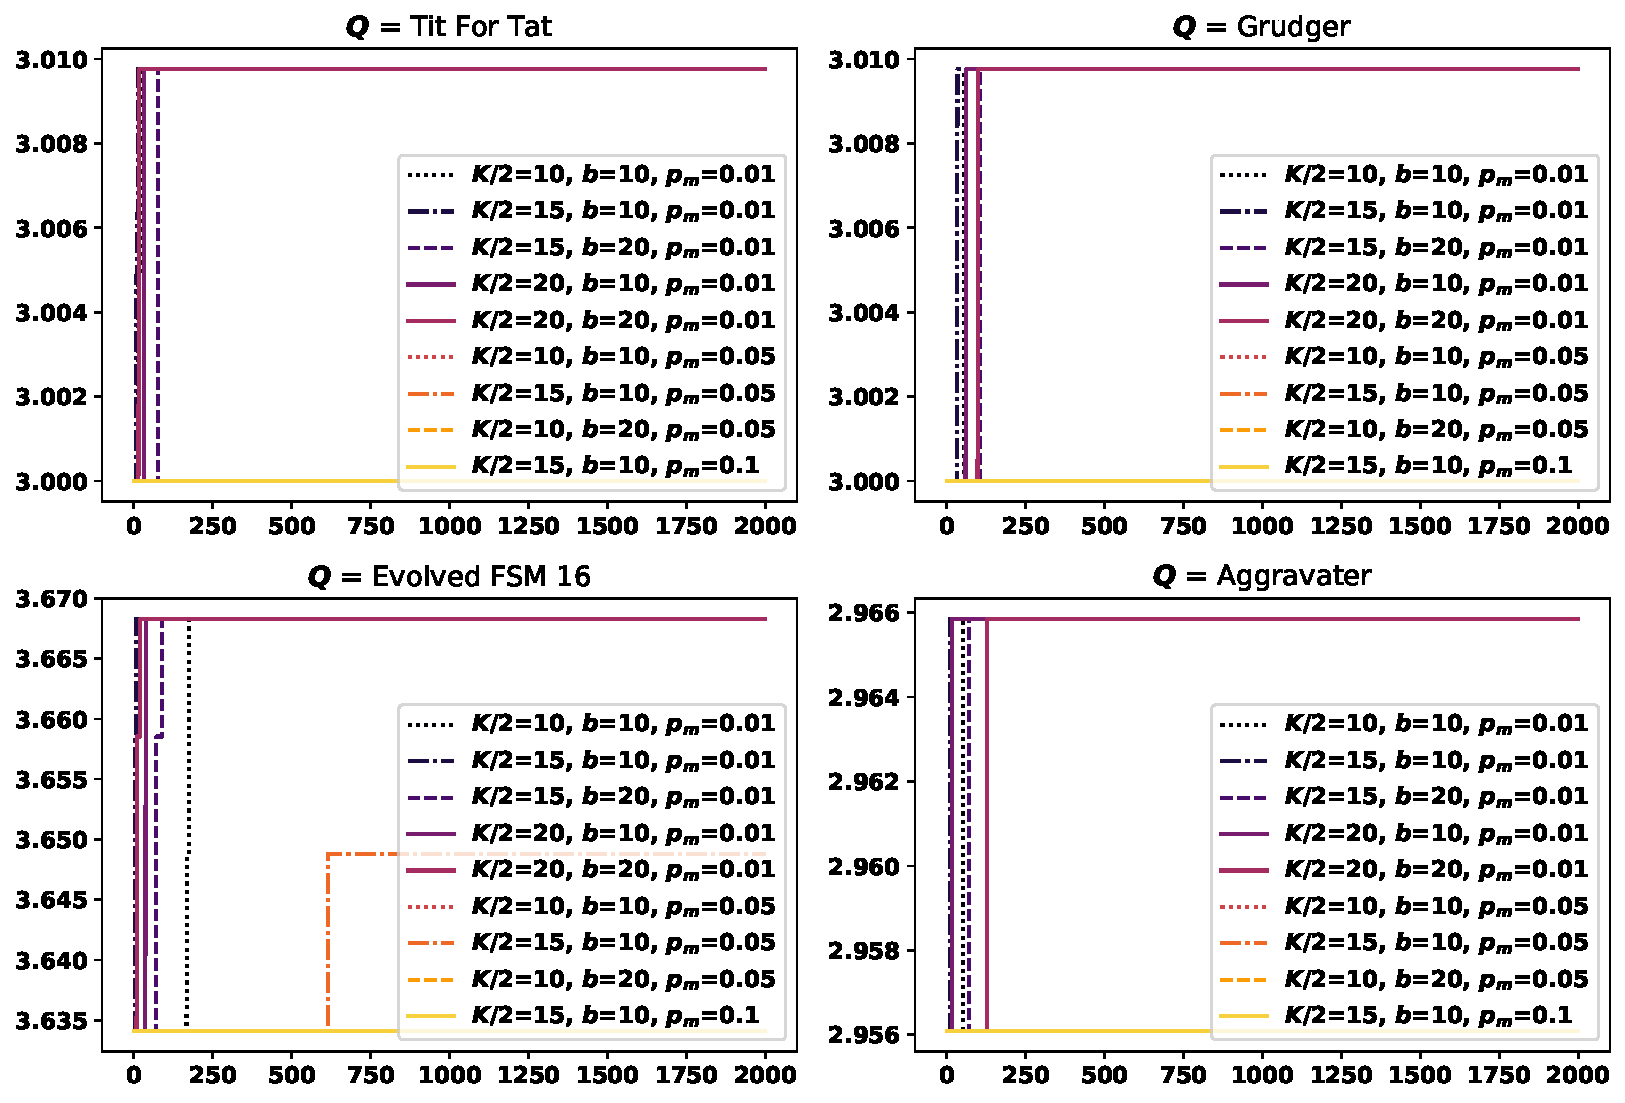
\includegraphics[width=.9\textwidth]{src/chapters/06/img/gas_results_per_trial.pdf}
    \caption{The highest score in a population over the generations for Tit For Tat,
    Grudger, FSM 16 and Aggravater. The selected trials capture the results
    of all the 18 trials for the given set of opponents.}\label{fig:ga_trials}
\end{figure}

Nevertheless % TODO Add a sentence or two here saying that even if a sequence doesn't converge it's still useful.

There are several trials that have managed to reach convergence,
and they did so in less than 200 generations. This is potentially the effect of a
non random initial population.
Figure~\ref{fig:ga_trials_to_500}
shows the highest score in a population over the generations for the four
strategies of Figure~\ref{fig:ga_trials} but only up to \(g_i = 500\). All trials
with a \(p_m=0.01\) reach convergence within the first 200 generations. The trial
which reaches convergence first (in the four demonstrated cases) is the trial
with the parameter values of \(K/2=15, b=10\) and \(p_m=0.1\).

\begin{figure}[!htbp]
    \centering
    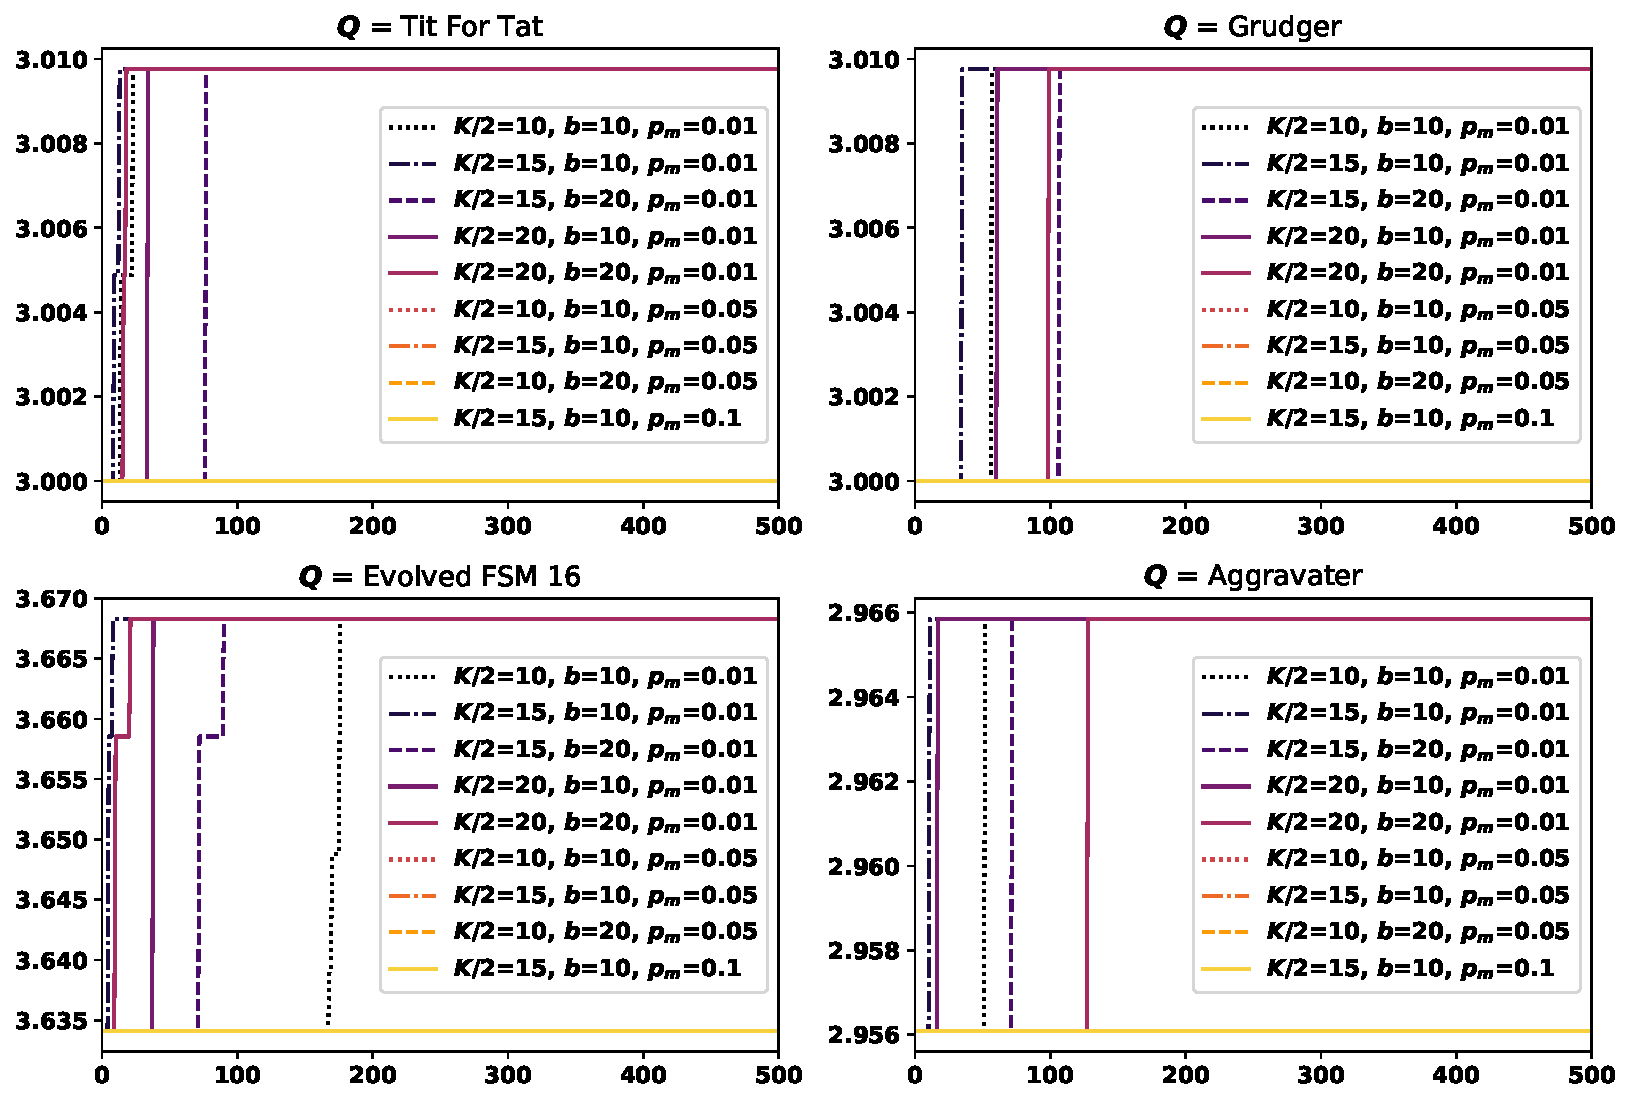
\includegraphics[width=.9\textwidth]{src/chapters/06/img/gas_results_per_trial_to_generation_500.pdf}
    \caption{The highest score in a population over the generations for Tit For Tat,
    Grudger, FSM 16 and Aggravater up to \(g_i = 500\).}\label{fig:ga_trials_to_500}
\end{figure}

There are a total of \deterministicstrategies deterministic strategies in the
collection of opponents and best response sequences were estimated for each.
Several of the known best response sequences have been manually checked and they
have been successfully estimated by the algorithm. These include best response
sequences to Tit For Tat, Grudger, Alternator, Pavlov and the Cycler strategies.

In section~\ref{section:ipd_as_sequences} is was explained that strategies can
have more than a single best response sequence. In the case of the strategy
Adaptive any strategy that cooperated twice in the opening 6 moves and defected
thereafter is a best response. The data collection has managed to successfully identify
multiple best responses to Adaptive, these are given by
Table~\ref{table:adaptive_best_responses}. Adaptive is not the only
deterministic strategy with multiple best response sequences. More specifically,
for the \deterministicstrategies deterministic opponents a total of \deterministicsequences best
response sequences were collected.

\begin{table}[!htbp]
    \resizebox{\textwidth}{!}{
    \begin{tabular}{lrrrrrrrrrrr}
\toprule
index &  gene 0 &  gene 1 &  gene 2 &  gene 3 &  gene 4 &  gene 5 &  gene 6 &  \(\dots\) &   gene 202 &  gene 203 &  gene 204 \\
\midrule
0     &       1 &       0 &       0 &       0 &       0 &       1 &       0 &  \(\dots\) &         0 &         0 &         0 \\
1     &       0 &       0 &       1 &       1 &       0 &       0 &       0 &  \(\dots\) &         0 &         0 &         0 \\
2     &       1 &       1 &       0 &       0 &       0 &       0 &       0 &  \(\dots\) &         0 &         0 &         0 \\
\bottomrule
\end{tabular}
}
    \caption{Best responses sequences estimated by the data collection process.
    Note that \(0\) corresponds to defection and \(1\) to cooperation.}
    \label{table:adaptive_best_responses}
\end{table}

An interesting questions that arises is: how diverse are the set of best response
sequences? Out of the \deterministicsequences sequences \stochasticuniquesequences are unique. A graphical
representation of these sequences is given by Figure~\ref{fig:brs_visualisation}.
The two distinct colours represent genes of \(C\) and \(D\). Overall, it can be
seen that there is diversity in the best response sequences, and they are not just
long sequences of either \(C\) or \(D\). A common trend appears to be a series
of defections at the last turns. In a finite IPD this is to expected. As it was
mentioned in Chapter~\ref{chapter:meta_tournaments}, as the likelihood of a
match ending in the following turn increases the effectiveness of defecting.

A total of \stochasticsequences sequences have been estimated for the stochastic opponents. From
these sequences, 66\% did indeed play against the correct seeded opponent and
achieved their respective scores at the final generation.

For instance for the strategy - seed combination of Champion - seed\(=9\) the highest score
achieved by a member of the population over the generations is given by
Figure~\ref{fig:champion_ga_score}. There is variation in the highest score
occurring over the generations with several increasing and decreasing peeks. However,
for most of the generations the highest score appears to be between \(3.80 - 3.82\).
The best response sequence retrieved by the data collection scored 3.82 against
Champion, and it reflected the score of the sequence against Champion - seed\(=9\).

\begin{figure}[!htbp]
    \centering
    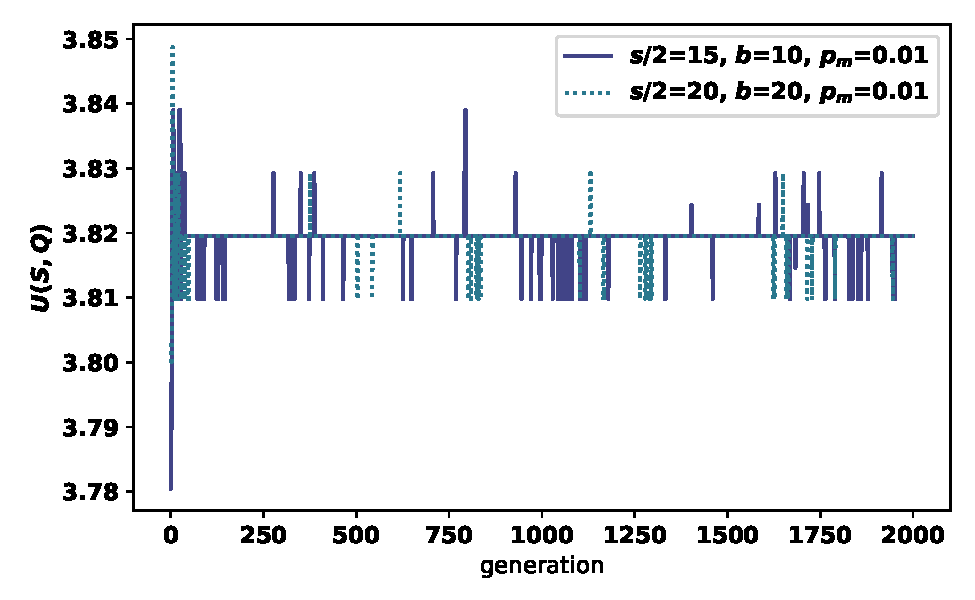
\includegraphics[width=.7\textwidth]{src/chapters/06/img/maximum_score_per_generation_champion.pdf}
    \caption{The maximum score a sequence achieved against Champion with seed 9
    over the generations. Each line represents a different GA trial. Only the
    GAs with \(p_m=0.01\) have been included.}\label{fig:champion_ga_score}
\end{figure}

There are stochastic opponents for which more variation occurred over the
generations. An example of that is Random. The highest score
of the population in a single GA trial, for opponent - seed combination Random -
seed\(=1\), is given by Figure~\ref{fig:random_ga_score}.
In the case of Random - seed\(=1\) the score of the best response sequence that
was collected was not the actual score the sequence scores against Random -
seed\(=1\).

\begin{figure}[!htbp]
    \centering
    \includegraphics[width=.7\textwidth]{src/chapters/06/img/maximum_score_per_generation_random.pdf}
    \caption{The maximum score a sequence achieved against Random - seed\(=1\)
    over the generations.}\label{fig:random_ga_score}
\end{figure}

From the \stochasticsequences sequences against stochastic strategies \stochasticuniquesequences are unique. A graphical representation of 1000 of
those sequences are given by Figure~\ref{fig:brs_visualisation_stochastic}.
Similar to the results of the best response sequences against deterministic
opponents the sequences are diverse.

\begin{figure}[!htbp]
    \begin{subfigure}{0.45\textwidth}
    \centering
    \includegraphics[width=.74\textwidth]{src/chapters/06/img/deterministic_best_responses.pdf}
    \caption{A graphical representation of best \deterministicsequences response sequence. These
    have been estimated using deterministic opponents.}\label{fig:brs_visualisation}
    \end{subfigure}\hfill
    \begin{subfigure}{0.45\textwidth}
    \centering
    \includegraphics[width=.74\textwidth]{src/chapters/06/img/stochastic_best_responses.pdf}
    \caption{A graphical representation of \stochasticsequences response sequence. These
    have been estimated using stochastic opponents.}\label{fig:brs_visualisation_stochastic}
    \end{subfigure}
\end{figure}

In summary, from the list of \numberofstrategiesbestsequences strategies
examined in this Chapter, 750 different opponent instances were simulated and a
total of \totalsequences best response sequences of length 205 were retrieved. The choice of
205 turns will be explained in the following Chapter. The best response sequences have
been archived and made available at~\cite{Glynatsi2020_sequences}.

\section{Chapter Summary}

This Chapter has explored the concept of best responses in the IPD game in the
form of static sequences of moves. It introduced an evolutionary algorithm,
Algorithm~\ref{algorithm:genetic_algorithm}, which can successfully identify
best response sequences.

The algorithm was executed to estimate best response sequences to the majority
of opponents listed in the APL. More specifically, a total of
\numberofstrategiesbestsequences opponents from APL were used. Several of the
strategies in the project are stochastic and computer seeded versions of these
strategies were used to explore their different behaviours. From the list of
\numberofstrategiesbestsequences opponents a total of 750 different behaviours
were simulated.

For the \deterministicstrategies deterministic strategies a total of \deterministicsequences
sequences, from which \deterministicuniquesequences were unique, were estimated. These sequences were not
just a set of trivial sequences of either \(C\) or \(D\). A common trait in the
best response sequences appeared to be a series of defection closer to the final
turns. For the seeded versions of the \stochasticstrategies stochastic opponents
the best response sequences are not guaranteed to have been captured due to issues related to PRNGs and multi threading.
Nevertheless, a total of \stochasticsequences sequences from which \stochasticuniquesequences are unique were
collected. Similar, these sequences are more diverse than just a series of
a single action. The \totalsequences sequences that were collected have been
archived and are available at \cite{Glynatsi2020_sequences}.

The main purpose of this Chapter has been to generate the bespoke data set,
which contains a large number of unique and diverse sequences,
so it can be used as training data set for Chapter~\ref{chapter:lstm}.

% \chapter{Training long short-term memory networks produces successful Prisoner's Dilemma strategies}\label{chapter:lstm}

\begin{center}
    The research reported in this Chapter has been carried out with:

    Axerod-Python library version: 4.2.0 \\
    Associated data set: \\ % TODO archive model weights
    This work was performed using the computational facilities of the Advanced Research
    Computing @ Cardiff (ARCCA) Division, Cardiff University.\\ \vspace{.5cm} 
\end{center}

\hrulefill

\section{Introduction}

In Chapter~\ref{chapter:meta_tournaments} it was mentioned that conceptualising
and introducing new strategies has been an important aspect of research to the
field. The aim of this Chapter is to introduce new IPD strategies based on an
archetype that has not received much attention in the literature.

In Chapter~\ref{chapter:meta_tournaments} it was concluded that one of the
properties successful strategies in a IPD competition need to have is
cleverness/complexity. Complexity can confer to adaptability, and adaptability
is important in performing well in diverse sets of environments. This was
established not only in Chapter~\ref{chapter:meta_tournaments} but also from the
results of Chapter~\ref{chapter:memory_one}. The set of complex strategies that
ranked highly across distinct tournaments in
Chapter~\ref{chapter:meta_tournaments} included strategies based on archetypes
such as finite state automata, hidden Markov models and \textit{artificial
neural networks} (ANNs).

ANNs have successfully been trained to play games other than the IPD such as
checkers~\cite{Chellapilla1999}, chess~\cite{Fogel2004} and
Go~\cite{Silver2016}. \textit{Feed forward networks} were firstly used to represent IPD
strategies in 1996 \cite{Harrald1996}. Feed forward networks have been used in
the literature ever since~\cite{Ashlock2008, Ashlock2006a, Darwen2001,
Franken2005}, and possibly the most successful ANN strategies in the game are
the ones introduced in~\cite{Harper2017}. The three ANN based strategies
in~\cite{Harper2017} ranked \(7^{th}\), \(9^{th}\), and \(11^{th}\) in a
tournament of 223 strategies.

A type of ANNs that have not received much attention in the literature are the
\textit{recurrent neural networks} (RNNs). RNNs are a type of neural networks
that include a feedback connection and are designed to work with inputs in
the form of sequences. RNNs were firstly considered as an archetype in 1996.
In~\cite{Sandholm1996} a RNN which considered a single previous step
as an input was trained via a \(Q\) learning algorithm to play against a single
opponent. The opponent was either the strategy \textsl{Tit For Tat} or another \(Q\)
learning strategy. The results of~\cite{Sandholm1996} although somewhat
promising, the RNN player learned to optimally play against \textsl{Tit For Tat},
they were limited.

The limitations of~\cite{Sandholm1996} could potentially have been due to the
limitations of the RNNs themselves. As it will be discussed later in
section~\ref{section:artificial_neural_networks}, RNNs
quickly became unable to learn due to the vanishing gradient problem.
To improve on the standard recurrent networks a new model called the
\textit{long short-term memory network} (LSTM) was introduced in~\cite{Hochreiter1997}.
Remembering information for long periods of time is 
their default behaviour, not something they struggle to learn.

LSTMs are a set of networks that have been proven to be successfully trained and
today are being used in a number of innovative applications such as time series
analysis \cite{Malhotra2015}, speech recognition~\cite{Sak2014} and prediction
in medical care pathways~\cite{Wang2018_lstm}. However, they have not received
attention in the IPD literature. The aim of this Chapter is to train and
introduce a number of strategies based on LSTMs. The training has been possible
due to the collection of best response sequences generated in
Chapter~\ref{chapter:best_response_sequence}.

A total of \lstmstrategies LSTMs based strategies are introduced in this
Chapter, and their performance is evaluated and compared in a meta tournament
analysis of \metatournamentslstm standard tournaments. The results demonstrate
that LSTM networks can be trained to successfully compete in IPD tournaments.
The rest of the Chapter is structured as follows:

\begin{itemize}
    \item section~\ref{section:artificial_neural_networks}, presents an
    introduction to artificial, recurrent and long short-term memory neural networks.
    \item section~\ref{section:training_a_rnn}, covers the architectural details
    of the LSTMs considered in this Chapter. The networks are trained to predict
    best response sequences. This is done not only on the entire data set
    generated by the collection of best response sequences, but also for three
    distinct sub sets of the collection.
    \item section~\ref{section:rnn_strategy_validation}, evaluates and compares
    the performance of \lstmstrategies LSTMs strategies in
    \metatournamentslstm standard IPD computer tournaments.
\end{itemize}

\section{Artificial, recurrent and long short-term memory neural networks}\label{section:artificial_neural_networks}

ANNs are computing systems vaguely inspired by the biological neural networks
that constitute brains. As stated in~\cite{Jain1996} the research on ANNs
has experienced three periods of extensive activity. The first peak was in the
1940s. The work of~\cite{McCulloch1943} opened the subject by creating a
computational model for neural networks. The second peak occurred in 1960s with
the introduction of the perceptron~\cite{Rosenblatt1958}. The perceptron is a
linear binary classifier and in the 1960s in was shown that it could be used to
learn to classify simple shapes with \(20\times20\) pixels input. However, it
was impossible for the perceptron to be extended to classification tasks with
many categories. The limitations of the model were presented
in~\cite{Minsky1969} which halted the enthusiasm of most researchers in ANNs,
resulting in no activity in the field for almost 20 years. The third peak occurred
in the early 1980s with the introduction of the back propagation algorithm for
multilayered networks~\cite{Werbos1974}. Though the algorithm was initially
proposed by~\cite{Werbos1974} it has been reinvented several times and it was
popularised by~\cite{McClelland1986}. Following the introduction of the
algorithm and the ability to now train more complex models, ANNs have received
considerable interest and are being used today in a number of applications,
good review articles include~\cite{Abiodun2019, Li2010, Mohanraj2015, Shahid2019}.

ANNs based on the connection pattern can be grouped into two categories:

\begin{itemize}
    \item Feed forward networks.
    \item Recurrent or feedback networks.
\end{itemize}

ANNs can be viewed as weighted directed graphs in which artificial neurons are
nodes and directed edges, with weights, are connections between the neuron
outputs and the neuron inputs~\cite{Jain1996}. This is demonstrated by Figure~\ref{fig:ann}.
In feed forward networks the
graphs have no loops, whereas in recurrent networks loops occur because of feedback
connections.

\begin{figure}[!htbp]
    \centering
    \includestandalone[width=.6\textwidth]{src/chapters/07/tex/standard_neural_network_diagram}
    \caption{A generic representation of an ANN.}\label{fig:ann}
\end{figure}

A graphical representation of a feed forward network with a single hidden layer
is given by Figure~\ref{fig:feedforward_network}.

\begin{figure}[!htbp]
    \centering
    \includestandalone[width=.5\textwidth]{src/chapters/07/tex/neural_network}
    \caption{Graphical representation of an feed forward network.}\label{fig:feedforward_network}
\end{figure}

A feed forward network is composed by an input layer, hidden layers, and an
output layer~\cite{Jain1996, Krose1993}. The input is a vector \(x\). The dimensionality, or
number of nodes of the input layer is dependent on the dimensionality of \(x\).
Each element of the input vector is connected to the hidden layer via a set of
learned weights. The hidden layer also consists of nodes. The number of
nodes of the hidden layer is an architectural decision. The \(j^{\text{th}}\)
hidden node outputs,

\[h_j = \phi (\sum_{i} w_{ij} x_{i}), \text{where } \phi  \text{ is an activation function}.\]

Frequently used activation functions~\cite{Karlik2011, Krose1993} include:

\begin{itemize}
    \item The sigmoid function \(\sigma(x)\) which squashes numbers into the range \([0, 1]\).
    \item The hyperbolic tangent, \(tanh(x)\) which squashes numbers into the range \([-1, 1]\).
    \item The rectified linear unit, \(ReLU(x)=max(0,x)\).
\end{itemize}

The hidden layer in turn is fully connected to an output layer, where the
\(j^{\text{th}}\) output node outputs,

\[y_{j} = \sum_{i} v_{ij} h_{i}.\]

Feed forward networks make predictions using forward propagation which in matrix
notation is described by,

\begin{align}\label{eq:neural_network_equations}
h & = \phi(Wx) \\ \label{eq:neural_network_equations_two}
\hat{y} & = \text{softmax}(Vh)
\end{align}

where \(W\) is a weight matrix connecting the input and hidden layers, \(V\) is
a weight matrix connecting the hidden and output layers and the output layer
transforms the raw scores to a probability via a \textit{softmax function}.

The softmax function, referred to also as softargmax~\cite{Goodfellow2016} or
normalised exponential function~\cite{Bishop2006}, is a function that normalises
a vector of \(M\) real numbers to a probability distribution consisting of \(M\)
probabilities proportional to the exponentials of the input numbers. The
normalisation ensures that the sum of the components of the output vector is 1.
The softmax function, denoted as \(s(x_i)\),
is defined by Equation~(\ref{eq:softmax}).

\begin{equation}\label{eq:softmax}
    s(x_i) = \frac{e^{x_i}}{\sum\limits_{m=1}^{M} e^{x_m}} \text{ for } i \in 1, \dots, M.
\end{equation}

\(W\) and \(V\) are the learning parameters of the network. Their dimensionality
depends on the dimensionality of network's layers. For example if \(x\) and \(\hat{y}\)
were 2 dimensional and the hidden layer had 500 nodes then \(W \in \R^{2 \times 500}\)
and \(V \in \R^{500 \times 2}\). Increasing the dimensionality of the hidden
layer corresponds to larger number of learning parameters.

To train an ANN a set of values for the learning parameters need to be found so
that the error on the training data is minimised~\cite{Gurney2007}. The function that measures
error is called the \textit{loss function}.
An example of a loss functions is the
\textit{cross entropy}, denoted as \(L(y, \hat{y})\) where \(\hat{y}\) is the
prediction and \(y\) the true output. For \(M\) training examples and \(K\)
classes the cross entropy error is given by Equation~(\ref{eq:cross_entropy}).

\begin{equation}\label{eq:cross_entropy}
    L(y, \hat{y}) = - \frac{1}{M} \sum_{m\in M} \sum_{k \in K} y_{m, k} \text{log}(\hat{y}_{m, k})
\end{equation}

The minimum of the loss function is calculated using the gradient descent algorithm
\cite{Ruder2016}. The gradient descent algorithm relies on the gradients which
are the vector of derivatives of the loss function with respect to the learning
parameters. Thus \(\frac{\partial{L}}{\partial{W}}\) and
\(\frac{\partial{L}}{\partial{V}}\). These gradients are calculated with the
back propagation algorithm~\cite{Wythoff1993} which is a way of efficiently
calculating the gradients starting from the output.

According~\cite{Ruder2016} to there are variants of the gradient descent which
differ in how much data is used to compute the gradient of the objective
function. Using the gradient descent algorithm, the weights are updated
incrementally after each pass over the training data set. In contrast, the
stochastic gradient descent performs a parameter update for each training
example. This work uses a variant of the stochastic gradient descent called the
Adaptive Moment Estimation (Adam) algorithm~\cite{Kingma2014}.

An extension of feed forward networks are recurrent networks. RNNs are
capable of processing variable length sequences of inputs. Sequences are data
samples over a number of time steps. RNNs can receive sequence inputs and output
sequences of the same length, using their internal state/knowledge to a make a
prediction on the input at time \(t\) based on the decisions made at the
previous time steps.

A graphical representation of a RNN is given by
Figure~\ref{fig:rnn}. The loop represents that information can be passed
down from one step of the network to the next. RNNs can be thought of as
multiple copies of the same network each passing a message to a successor, which
is also demonstrated by Figure~\ref{fig:rnn}.

\begin{figure}[!htbp]
    \centering
    \includestandalone[width=\textwidth]{src/chapters/07/tex/recurrent_neural_network}
    \caption{Graphical representation of a RNN.}\label{fig:rnn}
\end{figure}

In RNNs information is passed down by using,

\begin{equation*}
    h_t = \phi(Wx_t + Uh_{t-1})
\end{equation*}

where \(h_{t-1}\) is the hidden state computed at time \(t-1\) multiplied by
some weight vector \(U\). In matrix notation RNNs are described by,

\begin{align}\label{eq:recurrent_neural_network_equations}
    h_t & = \phi(Wx_t + Uh_{t-1}) \\
    \hat{y}_t & = \text{softmax}(Vh_t).
\end{align}

Unfortunately in practice RNNs quickly become unable to learn to connect the
information. The longer the sequences, the higher the chance that
the back propagation gradients either accumulate and explode or vanish down to
zero. The fundamental difficulties of RNNs were explored in depth
by~\cite{Bengio1994}. As stated in~\cite{Hochreiter1997}, although RNNs are
theoretically fascinating there was no clear practical advantage over feed
forward networks.

A network specifically designed to avoid the long-term dependency problem was
introduced by~\cite{Hochreiter1997}, called the long short-term memory
network.
The core idea to LSTMs is the \textit{cell state} also referred to as the
long term memory, denoted as \(C_t\). The cell state is a vector designed to pass down
information with only a few carefully regulated changes being applied to it
by structures called \textit{gates}. Gates are composed of a sigmoid neural
net layer and a point wise multiplication operator. In order to explain
the cell gate and subsequently how LSTMs make predictions consider
a LSTM's hidden layer at time step \(t\) given by Figure~\ref{fig:lstm_cell}.

\begin{figure}[!htbp]
    \centering
    \includestandalone[width=.7\textwidth]{src/chapters/07/tex/lstm_cell}
    \caption{An LSTM hidden layer at time step \(t\).}\label{fig:lstm_cell}
\end{figure}

The cell state and hidden state from the previous time step are fed back
into the network. Initially, the network decides what information from the
previous cell state is to be discarded. This decision is made by the
\textit{forget state}. The forget state considers the hidden state at time
\(t-1\) and the input at time \(t\),

\begin{equation}\label{eq:forget_gate}
    f_{t} = \sigma(W_{f}x_{t} + U_{f}h_{t-1}).
\end{equation}

The forget gate outputs a number between 0 and 1 or each number in the cell
state \(C_{t-1}\). A 1 represents ``keep this'' while a 0 represents ``forget
this''.

Secondly, the network decides what information is going to be stored at the
cell gate. There are two parts to this. Firstly, the input gate decides which values
are going to be updated,

\begin{equation}\label{eq:input_gate}
    i_{t} = \sigma(W_{i}x_{t} + U_{i}h_{t-1}).
\end{equation}

and secondly, a tanh layer creates a vector of candidate values denoted as
\(\tilde{C}_{t}\) that could be added to the cell state. \(\tilde{C}_{t}\) 
is given by Equation~(\ref{eq:candidate_set_for_cell_state}).

\begin{equation}\label{eq:candidate_set_for_cell_state}
    \tilde{C}_{t} = tanh(W_{c}x_{t} + U_{c}h_{t-1}).
\end{equation}

The cell state \(C_{t-1}\) is multiplied by \(f_{t}\), forgetting the values
which have been decided to be discarded. The new candidate values are scaled by how
much information has been decided to keep from the input. Thus,

\begin{equation}\label{eq:cell_gate}
    C_{t} = f_{t} C_{t-1} + i_{t} \tilde{C}_{t}.
\end{equation}

The LSTM outputs a hidden state at each time step which is based on the current
cell state. Initially, the cell state goes through a tanh function and then it
is multiplied by a sigmoid gate that decides which parts to output from the cell
state,

\begin{align}\label{eq:outpu_gate}
    o_{t} & = \sigma(W_{o}x_{t} + U_{o}h_{t-1}), \\
    h_{t} & = o_{t} * tanh(C_{t}).
\end{align}

This process is being carried out for each time step of the input sequence. At
each time step both the cell state and hidden state are feed back into the
network. The hidden state can also be used to make a prediction at each time
step as demonstrated by Figure~\ref{fig:lstm}.

\begin{figure}[!htbp]
    \centering
    \includestandalone[width=\textwidth]{src/chapters/07/tex/lstm}
    \caption{Graphical representation of an LSTM network.}\label{fig:lstm}
\end{figure}

LSTMs unique architecture allows them to learn longer-term dependencies and to
be trained using the back propagation algorithm. Hence, they are an exceptional
model for sequential data and this is why they were chosen here. As it was described in
Chapter~\ref{chapter:best_response_sequence}, the actions of IPD strategies can
be defined as sequences, and therefore a collection of best response sequences was
generated using a heuristic method. In section~\ref{section:training_a_rnn} a
variety of LSTM networks are trained to predict these best response sequences.

\section{Training LSTM networks to predict best response sequences}\label{section:training_a_rnn}

LSTM are trained in a supervised fashion on a set of training sequences. The
purpose of training a network in this Chapter is so it can learn to play
optimally against IPD strategies. For that reason the networks are going to be
trained on the collection of best response sequences generated in
Chapter~\ref{chapter:best_response_sequence}.

The training inputs are the actions of a given strategy for \(N\) turns. The
expected outputs are the responses to those \(N\) actions by the opponent's best
response sequence. Each best response sequence, from
Chapter's~\ref{chapter:best_response_sequence} collection, corresponds to 204
expected outputs. This is done so that each sample captures a match between a
strategy and its best response for turns in a match. Specifically
for \(N \in {1, 204}\).

Consider the actions of the strategy Adaptive and its best response, as
presented in section~\ref{section:the_collection_of_best_response_sequences},
given by Table~\ref{table:adaptive_vs_best_response_binary_lstm}.

\begin{table}[htbp]
    \centering
    \begin{tabular}{cccccccccccccccc}
        & \textbf{1} & \textbf{2} & \textbf{3} & \textbf{4}  & \textbf{5} & \textbf{6} & \textbf{7} & \textbf{8} & \textbf{9} & \textbf{10} & \textbf{11} &  \textbf{12} & \(\dots\)  & \textbf{204} &  \textbf{205} \\ 
        \midrule
        Adaptive & 1 & 1 & 1 & 1 & 1 & 1 & 1 & 0 & 0 & 0 & 0& 1& \(\dots\) & 1 & 1 \\
        \(S^*\) & 1 & 1 & 0 & 0 & 0 & 0 & 0 & 0 & 0 & 0 & 0 & 0& \(\dots\) & 0 & 0 \\ \bottomrule
    \end{tabular}
    \caption{The actions of the strategy Adaptive against one of the best response sequences
    to the strategy. Note that \(0 \to D\) and \(1 \to C\).}\label{table:adaptive_vs_best_response_binary_lstm}
\end{table}

Initially the highest dimensionality a training sample based on
Table~\ref{table:adaptive_vs_best_response_binary_lstm} can have is 204.
This is because the expected output to Adaptive's action in turn 1 is
the action of the best response sequence at turn 2. Moreover, the expected
output to the Adaptive's \(204^{\text{th}}\) action is the best response's
\(205^{\text{th}}\) action. This is demonstrated by
Figure~\ref{fig:input_output_example}.

\begin{figure}[!htbp]
    \centering
    \includestandalone[width=\textwidth]{src/chapters/07/tex/output}
    \caption{An example of a networks input and output of \(t=204\). The last
    action of Adaptive as well as the first action of the best
    response sequence are discarded.}\label{fig:input_output_example}
\end{figure}

Secondly, in order to train the networks on different input lengths the training
sample of Figure~\ref{fig:input_output_example} is transformed to 204 samples.
This is done by considering all the possible IPD matches between
the pair where the number of turns \(N \in [1, 204]\). For example
Table~\ref{table:adaptive_vs_best_response_binary_lstm} corresponds to the
training samples given by Equation~(\ref{eq:sequence_to_sequence_inputs_outputs_example}).

\begin{align}\label{eq:sequence_to_sequence_inputs_outputs_example}
x = & \begin{bmatrix} 1 \end{bmatrix} &\to & & 
y = & \begin{bmatrix} 1 \end{bmatrix} \nonumber \\
x = & \begin{bmatrix} 1 & 1 \end{bmatrix} &\to & & 
y = & \begin{bmatrix} 1 & 1 \end{bmatrix} \nonumber \\
x = & \begin{bmatrix} 1 & 1 & 1 \end{bmatrix} &\to & & 
y = & \begin{bmatrix} 1 & 1 & 0 \end{bmatrix} \nonumber \\
x = & \begin{bmatrix} 1 & 1 & 1 & 1 \end{bmatrix} &\to & & 
y = & \begin{bmatrix} 1 & 1 & 0 & 0 \end{bmatrix} \\
x = & \begin{bmatrix} 1 & 1 & 1 & 1 & 1 \end{bmatrix} &\to & & 
y = & \begin{bmatrix} 1 & 1 & 0 & 0 & 0 \end{bmatrix} \nonumber \\
x = & \begin{bmatrix} 1 & 1 & 1 & 1 & 1 & 1\end{bmatrix} &\to & & 
y = & \begin{bmatrix} 1 & 1 & 0 & 0 & 0 & 0\end{bmatrix} \nonumber \\
x = & \begin{bmatrix} 1 & 1 & 1 & 1 & 1 & 1 & 0 \end{bmatrix} &\to & & 
y = & \begin{bmatrix} 1 & 1 & 0 & 0 & 0 & 0 & 0 \end{bmatrix} \nonumber \\
\vdots & & & & \vdots \nonumber
\end{align}

Subsequently, the training data set retrieved from the collection of best
responses has a total of \(\totalsequences \times 204 = \trainingpoint\)
training samples.

Two types of LSTMs have been trained in this Chapter. These are referred to as:

\begin{itemize}
    \item The sequence to sequence (StoS) network.
    \item The sequence to probability (StoP) network.
\end{itemize}

Both networks take as input a sequence of actions. The StoS network outputs a
response to each time step of the input sequence, thus attempting to recover the entire best response sequence. The StoP network only outputs
a response to the sequence at the last time step, thus only attempting to figure out what comes next.
Both networks indicate the predicted action with a probability of cooperating.
A graphical representation of the two networks are given by
Figures~\ref{fig:sequence_to_sequence} and \ref{fig:sequence_to_probability}.

\begin{figure}[!htbp]
    \centering
    \includestandalone[width=\textwidth]{src/chapters/07/tex/sequence_to_sequence}
    \caption{A graphical representation of the StoS LSTM network.}\label{fig:sequence_to_sequence}
\end{figure}

\begin{figure}[!htbp]
    \centering
    \includestandalone[width=\textwidth]{src/chapters/07/tex/sequence_to_probability}
    \caption{A graphical representation of the StoP LSTM network.}\label{fig:sequence_to_probability}
\end{figure}

The StoS network is trained on samples in the form of
Equation~(\ref{eq:sequence_to_sequence_inputs_outputs_example}), whereas the
StoP network is trained on sample in the form of
Equation~(\ref{eq:sequence_to_probability_inputs_outputs_example}).

\begin{align}\label{eq:sequence_to_probability_inputs_outputs_example}
x = & \begin{bmatrix} 1 \end{bmatrix} &\to & & 
y = & \begin{bmatrix} 1 \end{bmatrix} \nonumber \\
x = & \begin{bmatrix} 1 & 1 \end{bmatrix} &\to & & 
y = & \begin{bmatrix} 1 \end{bmatrix} \nonumber \\
x = & \begin{bmatrix} 1 & 1 & 1 \end{bmatrix} &\to & & 
y = & \begin{bmatrix} 0 \end{bmatrix} \nonumber \\
x = & \begin{bmatrix} 1 & 1 & 1 & 1 \end{bmatrix} &\to & & 
y = & \begin{bmatrix} 0 \end{bmatrix} \\
x = & \begin{bmatrix} 1 & 1 & 1 & 1 & 1 \end{bmatrix} &\to & & 
y = & \begin{bmatrix} 0 \end{bmatrix} \nonumber \\
x = & \begin{bmatrix} 1 & 1 & 1 & 1 & 1 & 1\end{bmatrix} &\to & & 
y = & \begin{bmatrix} 0 \end{bmatrix} \nonumber \\
x = & \begin{bmatrix} 1 & 1 & 1 & 1 & 1 & 1 & 0 \end{bmatrix} &\to & & 
y = & \begin{bmatrix} 0 \end{bmatrix} \nonumber \\
\vdots & & & &\vdots \nonumber
\end{align}

\subsection{Building the networks with Keras}

There are many open source libraries that allow the creation of deep neural nets
in Python, without having to explicitly write the code from scratch. As stated
in~\cite{Vasilev2019} the three most popular are
TensorFlow~\cite{TensorFlow2015}, Keras~\cite{Chollet2015}, and
PyTorch~\cite{pytorch}. Keras is a high level neural net Python library that
runs on top of TensorFlow. Though Keras' performance is comparatively slower
than TensorFlow and PyTorch, Keras has a simple architecture and it is more
readable and concise. Keras has been used in several academic works such
as~\cite{Barbastathis2019, Mei2018, Soffer2019}, and is also used here to
construct and train the networks.

The Python code for implementing the StoS model is given by
Figure~\ref{fig:keras_sequence_to_sequence}. In line 12 the model is defined to
be of the \mintinline{python}{Sequential} class. This mean that the model will
be constructed layer by layer. The StoS network has a single LSTM layer with 100
nodes. The input to the LSTM network is not of a fixed length and there a single
time step between the elements of each input sequence. This is defined by the
argument \mintinline{python}{input_shape=(None, 1)}. The LSTM layer outputs a
hidden state at each time step. Initially, the hidden states go through a
dropout layer. The dropout layer is a simple and yet efficient method to reduce
overfitting by randomly dropping out nodes of the hidden
states~\cite{Baldi2013}. Finally, the hidden states are transformed into
probabilities via a sigmoid layer. There are a total of 41301 learning
parameters to the StoS model.

\begin{figure}[!htbp]
\begin{usagepy}
>>> from keras.models import Sequential

>>> from keras.layers import (
...     Dense,
...     Dropout,
...     CuDNNLSTM,
... )

>>> num_hidden_cells = 100
>>> drop_out_rate = 0.2

>>> model = Sequential()

>>> model.add(
...    CuDNNLSTM(
...        num_hidden_cells, return_sequences=True, input_shape=(None, 1))
... )

>>> model.add(Dropout(rate=drop_out_rate))

>>> model.add(Dense(1, activation="sigmoid"))
>>> model.summary()
Model: "sequential_1"
_________________________________________________________________
Layer (type)                 Output Shape              Param #   
=================================================================
cu_dnnlstm_1 (CuDNNLSTM)     (None, None, 100)         41200     
_________________________________________________________________
dropout_1 (Dropout)          (None, None, 100)         0         
_________________________________________________________________
dense_1 (Dense)              (None, None, 1)           101       
=================================================================
Total params: 41,301
Trainable params: 41,301
Non-trainable params: 0
_________________________________________________________________

\end{usagepy}
\caption{Python code for implementing the StoS LSTM with Keras.}\label{fig:keras_sequence_to_sequence}
\end{figure}

Regarding the dimensionality of the hidden layer there is no direct answer as to
what is the optimal number of nodes. Several methods for determining the
dimensionality include experimentation, intuition and building on the work of
others. A common practice is that the dimensionality of the hidden layer is
smaller than the dimensionality of the input layer. The dimensionality of the
input layer changes from 1 to 204, and thus a number of 100 nodes was chosen
so that the dimensionality of the hidden layer is smaller 50\% of the times.

The Python code for implementing the StoP network with Keras is given by
Figure~\ref{fig:keras_sequence_to_probability}. The implementations of the
networks are similar, however, the StoP model contains 2 LSTM layers. The first
LSTM layer outputs the hidden states at each time step. In turn these are connected to
the second layer which only outputs the hidden state at final time step. The StoP
network has a higher number of learning parameters due to the two LSTM layers.
More specifically, there are 122101 learning parameters to the network.

\begin{figure}[!htbp]
\begin{usagepy}
>>> from keras.models import Sequential
>>> from keras.layers import (
...     Dense,
...     Dropout,
...     CuDNNLSTM,
... )

>>> num_hidden_cells = 100
>>> drop_out_rate = 0.2

>>> model = Sequential()

>>> model.add(
...     CuDNNLSTM(num_hidden_cells, return_sequences=True, input_shape=(None, 1))
... )

>>> model.add(CuDNNLSTM(num_hidden_cells))
>>> model.add(Dropout(rate=drop_out_rate))

>>> model.add((Dense(1, activation="sigmoid")))
>>> model.summary()
Model: "sequential_2"
_________________________________________________________________
Layer (type)                 Output Shape              Param #   
=================================================================
cu_dnnlstm_2 (CuDNNLSTM)     (None, None, 100)         41200     
_________________________________________________________________
cu_dnnlstm_3 (CuDNNLSTM)     (None, 100)               80800     
_________________________________________________________________
dropout_2 (Dropout)          (None, 100)               0         
_________________________________________________________________
dense_2 (Dense)              (None, 1)                 101       
=================================================================
Total params: 122,101
Trainable params: 122,101
Non-trainable params: 0
_________________________________________________________________

\end{usagepy}
\caption{Python code for implementing the StoP LSTM with Keras.}\label{fig:keras_sequence_to_probability}
\end{figure}

Keras includes two implementations for an LSTM layer. The class
\mintinline{python}{LSTM} and the class \mintinline{python}{CuDNNLSTM} which is
the class used here. \mintinline{python}{CuDNNLSTM} provides a faster
implementation of \mintinline{python}{LSTM} with the NVIDIA CUDA Deep Neural Network
library. The use of the \mintinline{python}{CuDNNLSTM} class means that the networks
can be trained on a graphics processing unit (GPU).

\subsection{High performance training}

Conventionally the execution of computer code happens on the central processing
unit (CPU). The CPU, also called main processor, is essentially the brain of any
computing device~\cite{Berger2005}. Architecturally the CPU is composed of just
a few cores designed to support an extremely broad variety of tasks.

A graphical processing unit (GPU), on the other hand, is composed of hundred of
cores designed to process a set of simpler and more identical computations in
parallel. GPUs were initially designed as dedicated graphical rendering
workhorses for computer games. However as stated in~\cite{Catanzaro2008},
graphics processors transitioned from their initial role to general purpose
engines for high throughput floating-point computation.

A CPU core is more powerful than a GPU core. A CPU core is designed to carry out
a variety of tasks one of which include computations, whereas GPUs are designed
exclusively for data computations. The vast majority of a CPUs power goes unused
by machine learning applications. Machine learning applications which perform
large numbers of computations on a vast amount of data can see huge performance
improvements when running on a GPU versus a CPU.

There are several manufacturers of GPUs. These include NVIDIA, AMD, Asus and
Intel. NVIDIA created a parallel computing architecture and platform for its
GPUs called CUDA~\cite{Harris2008}. CUDA programming model gave developers
access and the ability to express simple processing operations in parallel
through code. The vast majority of deep learning projects work exclusively with
NVIDIA GPUs because of the better software support NVIDIA provides. In 2005,
\cite{Steinkraus2005} presented the usage of GPUs in training a generic 2 layer
fully connected neural network. The first important work was later in
2008~\cite{Raina2009}. However, the usage of GPUs in machine learning was
popularised in 2012 by~\cite{Krizhevsky2012}.

Due to the time advantage, the training process of the networks was carried out
on a GPU. The training was performed using the computational facilities of the
ARCCA division, Cardiff University.

\subsection{Training data sets}

Section~\ref{section:training_a_rnn} covered the training data set used to train
the LSTM networks. There are a total of \trainingpoint training inputs and expected
outputs in the data set. In order to understand the effect of the training
samples on the LSTM strategies' performance the networks are trained on the
entire data set and on three unique subsets.

The subsets are based on three collection of opponents. These are a collection
of best performing strategies, strategies with ranks across a standard
tournament and a collection of basic strategies. The details of the subsets are
given by Table~\ref{table:training_data_sets}.
A list of the strategies' names used in each subset is given in the Appendix~\ref{appendix:training_sets_strategies}.

\newcolumntype{g}{>{\columncolor{Gray}}c}
\begin{table}[htb]
    \centering
    \resizebox{\textwidth}{!}{
    \begin{tabularx}{1.5\textwidth}{cgXg}
    \toprule
    Data set & \# of opponents & Explanation & \thead{\# of best response \\ sequences} \\
    \midrule
    all strategies & \numberofstrategiesbestsequences & The data set as presented in section~\ref{section:training_a_rnn}. & \totalsequences \\
    top performing strategies & \topstrategies & A data set constructed in the same way as the training data set but only with the best response sequences
    to \topstrategies strategies. These are the top performing strategies in a standard tournament of 218 opponents. & \topsequences \\
    strategies across ranks & \acrossstrategies & A data set generated only with the best response sequences to
    \acrossstrategies strategies whose ranks are across the 218 ranks of the standard tournament. & \acrosssequences\\
    basic strategies & \basicstrategies & A data set generated with the best response sequences to \basicstrategies strategies
    which are classified as a set of basic strategies in the APL. & \basicsequences \\
    \bottomrule
    \end{tabularx}}
    \caption{Training data sets used to train the LSTM networks. The IPD
    standard tournament with the 218 opponent has been carried out using APL version
    3.10.0. The results are available at~\cite{std_tournament_results}.}\label{table:training_data_sets}
\end{table}

\subsection{Training and validation}

The two different LSTM networks, StoS and StoP, are trained on four
different training sets. Thus, a total of \(4 \times 2 = \lstmnetworks\)
LSTM networks have been trained in this Chapter.

The networks were trained using the back propagation algorithm
and the Adam algorithm presented in
section~\ref{section:artificial_neural_networks}.
Due to the different size of the training data the networks have been trained
for a different number of epochs. The number of epochs is the number of times
the training algorithm has work through an entire training data set. The number
of epochs for each of the \lstmnetworks network is given by
Table~\ref{table:epochs}.

\begin{table}[!htbp]
    \begin{center}
    \resizebox{.9\textwidth}{!}{
        \begin{tabular}{lcccc}
\toprule
{} &  all strategies &  top strategies &  strategies across ranks &  basic strategies \\
\midrule
sequence to sequence    &           19999 &           83999 &                    39999 &            129999 \\
sequence to probability &            7999 &           74999 &                    39999 &             84999 \\
\bottomrule
\end{tabular}

    }
\end{center}
\caption{Number of epochs for each of the LSTM networks.}\label{table:epochs}
\end{table}

The StoP networks have a larger number of learning parameters. Subsequently,
their training corresponds to more computer time. It can been seen from
Table~\ref{table:epochs} that the StoP networks have been trained for less
epochs compared to the StoS networks.

At each training process the training data set is split into 80\% training samples
and 20\% test samples. At each epoch the loss function is calculated for both
the training and test samples. The loss function used to trained the networks
is the \textit{binary cross entropy}. In essence, the task of predicting IPD
actions is a binary classification problem as there can only be two classes:
cooperation or defection.

As discussed in section~\ref{section:artificial_neural_networks}, the loss
function is used to optimise the learning algorithm. The networks that will
be used as IPD strategies in the next section are the networks that achieved
the lowest loss value over the epochs. The weights of the best performing
networks have been archive and are available at. %TODO archive weights

Another measure which is being reported at each epoch is the accuracy. The accuracy
is calculated after the learning parameters have been determined and it is in
the form of a percentage. Accuracy is a measure of how accurate the predictions
are based on the expected output. Both the measures over the number of epochs
are given by Figures~\ref{fig:validation_sequence_to_sequence}
and~\ref{fig:validation_sequence_to_probability}.

In Figure~\ref{fig:validation_sequence_to_sequence} the loss and accuracy are
given for the StoS networks. Overall the StoS networks, regarding the training
data set, have maintained a high value of accuracy over the epochs. Whilst
training on the basic strategies there was a minor decrease, however, the
accuracy still remained over 0.85 (85\%). The loss function values have also
remained low over the epochs, for all the networks, with only a few spikes
occurring.

\begin{figure}[!htbp]
    \begin{subfigure}{\textwidth}
    \centering
    \includegraphics[width=.8\textwidth]{src/chapters/07/img/validation_plot_all_strategies.pdf}
    \end{subfigure}\hfill
    \begin{subfigure}{\textwidth}
    \centering
    \includegraphics[width=.8\textwidth]{src/chapters/07/img/validation_plot_top_strategies.pdf}
    \end{subfigure}
    \begin{subfigure}{\textwidth}
    \centering
    \includegraphics[width=.8\textwidth]{src/chapters/07/img/validation_plot_across_ranks_strategies.pdf}
    \end{subfigure}
    \begin{subfigure}{\textwidth}
    \centering
    \includegraphics[width=.8\textwidth]{src/chapters/07/img/validation_plot_basic_strategies.pdf}
    \end{subfigure}
    \caption{Loss function and accuracy of the networks based on the StoS network,
    over the number of epochs.}\label{fig:validation_sequence_to_sequence}
\end{figure}

For the StoP networks there appears to be more variation in the test loss and
accuracy, Figure~\ref{fig:validation_sequence_to_probability}. This is more evident
for the networks that were trained on the top strategies and the strategies
across ranks. This could indicate that the networks are overfitting. The StoP
network trained on the entire training data set has managed to maintained
a low loss value (at 0.5) and a training accuracy of 0.75. The most successfully
trained StoP network appears to be the network trained on the basic strategies.

\begin{figure}[!htbp]
    \begin{subfigure}{\textwidth}
    \centering
    \includegraphics[width=.8\textwidth]{src/chapters/07/img/validation_plot_classification_all_strategies.pdf}
    \end{subfigure}\hfill
    \begin{subfigure}{\textwidth}
    \centering
    \includegraphics[width=.8\textwidth]{src/chapters/07/img/validation_plot_classification_top_strategies.pdf}
    \end{subfigure}
    \begin{subfigure}{\textwidth}
    \centering
    \includegraphics[width=.8\textwidth]{src/chapters/07/img/validation_plot_classification_across_ranks_strategies.pdf}
    \end{subfigure}
    \begin{subfigure}{\textwidth}
    \centering
    \includegraphics[width=.8\textwidth]{src/chapters/07/img/validation_plot_classification_basic_strategies.pdf}
    \end{subfigure}
    \caption{Loss function and accuracy of the networks based on the StoP
    network, over the number of epochs.}\label{fig:validation_sequence_to_probability}
\end{figure}

This section has presented the \lstmnetworks trained LSTM networks of this thesis.
These networks are based on two different architectures and have been trained
on four different training data sets. The networks' validation based on the
training data sets was presented in this section. In the next section the networks
are evaluated as IPD strategies.

\section{Validation of LSTM based strategies using a meta tournament analysis}\label{section:rnn_strategy_validation}

This section evaluates the trained LSTM networks as IPD strategies.
A strategy class called the \mintinline{python}{LSTMPlayer} was implemented
in order for the networks, which are Keras models, to interact in an IPD match
simulated with APL. The source code for the \mintinline{python}{LSTMPlayer} is
given by Figure~\ref{fig:lstm_player_source_code}. The class has three input
arguments:

\begin{itemize}
    \item A Keras model. The input models are the \lstmnetworks trained LSTM networks
    presented in section~\ref{section:training_a_rnn}.
    \item A reshape history function. A function that reshapes the opponent's
    history to the appropriate LSTM input.
    \item The probability that the strategy opens with cooperation on the first turn denoted
    as \(p_o\). The LSTM networks can be used to predict the strategy's next
    action following the opponent's opening turn. Thus, the strategy's opening
    action must be manually defined.
\end{itemize}

Following the opening turn the LSTM strategy makes a prediction based on the
opponent's history. The strategy has an infinite memory because it needs to
remember all the actions made by the opponent. The prediction of the networks
correspond to the probability of cooperating. The LSTM strategy makes a deterministic
decision based on the predicted probability. It cooperates if the prediction
on the last time step is greater than 0.5, otherwise it defects.
In Section~\ref{sec:stochastic-lstm-strategies} the performance of strategy that
plays stochastically will be briefly discussed.

\begin{figure}[!htbp]
\begin{sourcepy}
import numpy as np

import axelrod as axl
from axelrod.random_ import random_choice
from keras.layers import LSTM, Dense, Dropout
from keras.models import Sequential

C, D = axl.Action.C, axl.Action.D


class LSTMPlayer(axl.Player):
    name = "The LSTM player"
    classifier = {
        "memory_depth": float("inf"),
        "stochastic": True,
        "inspects_source": False,
        "manipulates_source": False,
        "manipulates_state": False,
    }

    def __init__(self, model, reshape_history_funct, opening_probability=0.78):
        self.model = model
        self.opening_probability = opening_probability
        self.reshape_history_function = reshape_history_funct
        super().__init__()
        if opening_probability in [0, 1]:
            self.classifier["stochastic"] = False

    def strategy(self, opponent):
        if len(self.history) == 0:
            return random_choice(self.opening_probability)

        history = [action.value for action in opponent.history]
        prediction = float(
            self.model.predict(self.reshape_history_function(history))[0][-1]
        )

        return axl.Action(round(prediction))

    def __repr__(self):
        return self.name
\end{sourcepy}
\caption{Implementation of the \mintinline{python}{LSTMPlayer} class.}\label{fig:lstm_player_source_code}
\end{figure}

The \lstmnetworks trained LSTM networks are used to introduce \lstmstrategies
new IPD strategies. Each network corresponds to three distinct players with a
different opening move. More specifically, three different values of \(p_o\) are
used here. These are \(p_o = 0\), \(p_o = 1\) and \(p_o = 0.78\). The
probability 0.78 is the probability that the best response sequences of Chapter
\ref{chapter:best_response_sequence} opens with a cooperation. Thus, a total of
\(8 \times 3 =  \lstmstrategies\) IPD strategies are evaluated in this section.

The performance of the LSTM strategies are evaluated and compared in
\metatournamentslstm standard tournaments similarly to Chapter~\ref{chapter:meta_tournaments}. The process of collecting the
tournaments results for each strategy is given by
Algorithm~\ref{algorithm:meta_tournament_lstm_validation}.

\begin{algorithm}[!htbp]
    \setstretch{1.35}
    \ForEach{\text{seed} $\in [0, 300]$}{
        $s \gets \text{randomly select integer}\in [s_{min}, s_{max}]$\;
        $\text{players} \gets  \text{randomly select $s$ players}$\;
        $\text{players} \gets  \text{players} + \text{LSTM strategy}$\;
        $s \gets s + 1$\;
        $k \gets  50$\;
        $n \gets  200$\;
        \vspace{0.4cm}
        $\text{result standard}$ $\gets$ Axelrod.tournament$(\text{players}, n, k)$\;}
    \KwRet{result standard}\;
    \caption{Standard tournament result summary collection algorithm}
    \label{algorithm:meta_tournament_lstm_validation}
\end{algorithm}

For each trial a random size \(s \in [5, 10]\) is selected, and from the
\numberofstrategiesbestsequences strategies of Appendix, a random list of \(s\) strategies is chosen. %TODO fix Appendix of Chapter 6.
The LSTM player is then added
to the list of players, increasing the size to \(s + 1\). For the given list of
strategies a standard tournament of 200 turns is performed and repeated 50
times. The number of turns is fixed at 200. In
Chapter~\ref{chapter:best_response_sequence} the sequences were fixed to 205
turns which resulted in many best response sequences to defect on the last turn
as the match was coming to an end. To avoid a series of 
unconditional defections by the LSTM strategies their performance is evaluated
in  200 turns, which is a common number of turns used in the IPD literature~\cite{Axelrod1980a, Axelrod1980b, Harper2017, Knight2016}.

A total of \metatournamentslstm trials of
Algorithm~\ref{algorithm:meta_tournament_lstm_validation} have been run. For
each trial a result summary (in the format of Table~\ref{table:output_result})
is exported. Similarly to Chapter~\ref{chapter:meta_tournaments}, the performance of the strategies is evaluated on the normalised.
rank \(r\), and more specifically on the median normalised rank \(\bar{r}\). As
a reminder \(r\) is calculated as a strategy's rank divided by \(s-1\).

The \(\bar{r}\) of each of the \lstmstrategies strategies over the \metatournamentslstm
standard tournaments is given by Table~\ref{table:normalised_rank_lstm_tournaments}.

\begin{table}[!htbp]
    \begin{center}
    \resizebox{.9\textwidth}{!}{
        \begin{tabular}{lllllll}
\toprule
{} & \multicolumn{3}{c}{\textbf{sequence to sequence}} & \multicolumn{3}{c}{\textbf{sequence to probability}} \\
{} &                       $p_o=0$ &                       $p_o=1$ &                    $p_o=0.78$ &                       $p_o=0$ &                       $p_o=1$ &                    $p_o=0.78$ \\
\midrule
All strategies          &  \cellcolor{orange!67.0}0.667 &  \cellcolor{orange!22.0}0.222 &  \cellcolor{orange!33.0}0.333 &  \cellcolor{orange!78.0}0.778 &  \cellcolor{orange!33.0}0.333 &    \cellcolor{orange!50.0}0.500 \\
Top strategies          &  \cellcolor{orange!71.0}0.714 &  \cellcolor{orange!44.0}0.444 &    \cellcolor{orange!50.0}0.500 &    \cellcolor{orange!50.0}0.500 &  \cellcolor{orange!43.0}0.429 &  \cellcolor{orange!43.0}0.429 \\
Across ranks strategies &   \cellcolor{orange!75.0}0.750 &  \cellcolor{orange!67.0}0.667 &  \cellcolor{orange!68.0}0.683 &    \cellcolor{orange!50.0}0.500 &   \cellcolor{orange!25.0}0.250 &    \cellcolor{orange!30.0}0.300 \\
Basic strategies        &    \cellcolor{orange!80.0}0.800 &    \cellcolor{orange!60.0}0.600 &  \cellcolor{orange!62.0}0.625 &    \cellcolor{orange!80.0}0.800 &    \cellcolor{orange!30.0}0.300 &  \cellcolor{orange!43.0}0.429 \\
\bottomrule
\end{tabular}

    }
\end{center}
\caption{The median normalised ranks of the 24 LSTM strategies over the standard
tournaments. A \(\bar{r}\) closer to 0 indicates a more successful performance.}
\label{table:normalised_rank_lstm_tournaments}
\end{table}

The strategy with the lowest \(\bar{r}\) over the \metatournamentslstm
tournaments is the LSTM strategy based on the StoS network trained over the entire
training set with \(p_o=1\). The strategy achieved a \(\bar{r}\) of 0.222. The
second most successful performance is by the StoP based strategy trained against
the across the ranks strategies with \(p_o=1\). In
section~\ref{section:training_a_rnn} it was indicated that the specific network
was overfitting, however, as an IPD strategy the network outperforms any other
StoP strategies.

A few strategies have achieved a \(\bar{r}\)
close to 0.3. These include the StoS strategy trained on the entire data set
with \(p_o=0.78\), and the StoP strategies trained against all strategies,
across the ranks strategies, and against the basic strategies with \(p_o=1\),
\(p_o=0.78\) and \(p_o=1\) equivalently.

The LSTM strategies that open with cooperation outperform any other strategy,
based on the same LSTM networks. Overall, the best performing
strategies open with cooperation. The strategies that open with a probabilistic
cooperation perform better than the strategies that open with defection.
Interestedly, from Table~\ref{table:normalised_rank_lstm_tournaments} it is
indicated that the strategies trained on the subsets perform better when they
are based on the StoP model. There is no intuition as to why that is. The
StoP networks have more learning parameters and yet they perform better when
trained on the smaller training sets than the StoS network. The StoP
network, trained against the entire data set, has trained for the smallest
number of epochs. A topic of future work would be to train the specific network
for more epochs.

Figure~\ref{fig:normalised_rank_distributions_sequence_to_sequence} gives the
\(r\) distributions for the strategies based on the StoS network. All the
distributions for \(p_o=0\) have a median higher than 0.66, indicating that
those strategies on average perform in the bottom half of a tournament. The most
successful strategy is the strategy trained against all strategies with
\(p_o=1\). The strategy's distribution shows that the strategy ranked highly in
most of the tournament it participated with only a few exceptions. Even if when
\(p_o\) is lowered to 0.78 the strategy still performs adequately. The rest
of the distributions appear to have peaks either at 0.5 or closer to 1. A
statistical summary of the distributions are given by
Table~\ref{table:statistic_summary_s_to_s}.

\begin{figure}[!htbp]
    \begin{subfigure}{\textwidth}
    \includegraphics[width=\textwidth]{src/chapters/07/img/normalised_rank_all_strategies.pdf}
    \end{subfigure}
    \par\bigskip
    \begin{subfigure}{\textwidth}
    \includegraphics[width=\textwidth]{src/chapters/07/img/normalised_rank_top_strategies.pdf}
    \end{subfigure}
    \par\bigskip
    \begin{subfigure}{\textwidth}
    \includegraphics[width=\textwidth]{src/chapters/07/img/normalised_rank_across_ranks_strategies.pdf}
    \end{subfigure}
    \par\bigskip
    \begin{subfigure}{\textwidth}
    \includegraphics[width=\textwidth]{src/chapters/07/img/normalised_rank_basic_strategies.pdf}
    \end{subfigure}
    \caption{Normalised rank distributions for the strategies which are based on the StoS
    LSTM.}\label{fig:normalised_rank_distributions_sequence_to_sequence}
\end{figure}

\begin{table}[!htbp]
    \begin{center}
    \resizebox{\textwidth}{!}{
        \begin{tabular}{llrrrrrrrrrrrr}
\toprule
                 &            &  count &   mean &    std &  min &    10\% &    25\% &    50\% &    75\% &    95\% &  max &   skew &   kurt \\
\midrule
\rowcolor{Gray}
All strategies & $p_o=0$ &  300.0 &  0.620 &  0.278 &  0.0 &  0.200 &  0.429 &  0.667 &  0.839 &  1.000 &  1.0 & -0.523 & -0.587 \\
\rowcolor{Gray}
                 & $p_o=1$ &  300.0 &  0.295 &  0.252 &  0.0 &  0.000 &  0.111 &  0.222 &  0.458 &  0.779 &  1.0 &  0.702 & -0.251 \\
\rowcolor{Gray}
                 & $p_o=0.78$ &  300.0 &  0.368 &  0.265 &  0.0 &  0.000 &  0.143 &  0.333 &  0.560 &  0.833 &  1.0 &  0.433 & -0.647 \\
                 \midrule
Top strategies & $p_o=0$ &  300.0 &  0.655 &  0.273 &  0.0 &  0.250 &  0.500 &  0.714 &  0.875 &  1.000 &  1.0 & -0.629 & -0.436 \\
                 & $p_o=1$ &  300.0 &  0.461 &  0.274 &  0.0 &  0.090 &  0.222 &  0.444 &  0.667 &  0.875 &  1.0 & -0.029 & -0.940 \\
                 & $p_o=0.78$ &  300.0 &  0.509 &  0.255 &  0.0 &  0.167 &  0.333 &  0.500 &  0.704 &  0.876 &  1.0 & -0.158 & -0.710 \\
                 \midrule
\rowcolor{Gray}
Representative strategies & $p_o=0$ &  300.0 &  0.643 &  0.306 &  0.0 &  0.141 &  0.486 &  0.750 &  0.875 &  1.000 &  1.0 & -0.768 & -0.523 \\
\rowcolor{Gray}
                 & $p_o=1$ &  300.0 &  0.636 &  0.262 &  0.0 &  0.250 &  0.500 &  0.667 &  0.833 &  1.000 &  1.0 & -0.680 & -0.198 \\
\rowcolor{Gray}
                 & $p_o=0.78$ &  300.0 &  0.645 &  0.255 &  0.0 &  0.250 &  0.500 &  0.683 &  0.833 &  1.000 &  1.0 & -0.754 & -0.034 \\
                 \midrule
Basic strategies & $p_o=0$ &  300.0 &  0.728 &  0.263 &  0.0 &  0.333 &  0.600 &  0.800 &  1.000 &  1.000 &  1.0 & -0.949 &  0.229 \\
                 & $p_o=1$ &  300.0 &  0.556 &  0.283 &  0.0 &  0.143 &  0.375 &  0.600 &  0.778 &  1.000 &  1.0 & -0.365 & -0.803 \\
                 & $p_o=0.78$ &  300.0 &  0.579 &  0.280 &  0.0 &  0.167 &  0.375 &  0.625 &  0.800 &  1.000 &  1.0 & -0.435 & -0.772 \\
\bottomrule
\end{tabular}

    }
\end{center}
\caption{Statistics summary of the \(r\) distributions for the strategies
based on the StoS network.}\label{table:statistic_summary_s_to_s}
\end{table}

Figure~\ref{fig:normalised_rank_distributions_sequence_to_probability} gives the
\(r\) distributions for the strategies based on the StoP network. For \(p_o=0\)
the performance of the strategies remains poorly. The strategies that have been
trained against all strategies, across the ranks and basic strategies with
\(p_o=1\) appear to have won several of the tournaments they
participated in. The statistics summary of the distributions is given by
Table~\ref{table:statistic_summary_s_to_p}.

\begin{figure}[!htbp]
    \begin{subfigure}{\textwidth}
    \includegraphics[width=\textwidth]{src/chapters/07/img/normalised_rank_classification_all_strategies.pdf}
    \end{subfigure}
    \par\bigskip
    \begin{subfigure}{\textwidth}
    \includegraphics[width=\textwidth]{src/chapters/07/img/normalised_rank_classification_top_strategies.pdf}
    \end{subfigure}
    \par\bigskip
    \begin{subfigure}{\textwidth}
    \includegraphics[width=\textwidth]{src/chapters/07/img/normalised_rank_classification_across_ranks_strategies.pdf}
    \end{subfigure}
    \par\bigskip
    \begin{subfigure}{\textwidth}
    \includegraphics[width=\textwidth]{src/chapters/07/img/normalised_rank_classification_basic_strategies.pdf}
    \end{subfigure}
    \caption{Normalised rank distributions for the strategies which are based on the StoP
    LSTM.}\label{fig:normalised_rank_distributions_sequence_to_probability}
\end{figure}

\begin{table}[!htbp]
    \begin{center}
    \resizebox{.9\textwidth}{!}{
        \begin{tabular}{llrrrrrrrrrrrr}
\toprule
                 &            &  count &   mean &    std &  min &    10\% &    25\% &    50\% &    75\% &    95\% &  max &   skew &   kurt \\
\midrule
\rowcolor{Gray}
All strategies & $p_o=0$ &  300.0 &  0.720 &  0.254 &  0.0 &  0.333 &  0.571 &  0.778 &  0.900 &  1.000 &  1.0 & -0.860 &  0.056 \\
\rowcolor{Gray}
                 & $p_o=1$ &  300.0 &  0.339 &  0.244 &  0.0 &  0.000 &  0.125 &  0.333 &  0.500 &  0.800 &  1.0 &  0.458 & -0.280 \\
\rowcolor{Gray}
                 & $p_o=0.78$ &  300.0 &  0.471 &  0.255 &  0.0 &  0.125 &  0.286 &  0.500 &  0.625 &  0.875 &  1.0 & -0.064 & -0.696 \\
                 \midrule
Top strategies & $p_o=0$ &  300.0 &  0.491 &  0.305 &  0.0 &  0.000 &  0.200 &  0.500 &  0.714 &  1.000 &  1.0 & -0.131 & -1.140 \\
                 & $p_o=1$ &  300.0 &  0.417 &  0.283 &  0.0 &  0.000 &  0.167 &  0.429 &  0.600 &  0.875 &  1.0 &  0.157 & -0.974 \\
                 & $p_o=0.78$ &  300.0 &  0.432 &  0.277 &  0.0 &  0.000 &  0.200 &  0.429 &  0.625 &  0.876 &  1.0 &  0.109 & -0.891 \\
                 \midrule
\rowcolor{Gray}
Across ranks strategies & $p_o=0$ &  300.0 &  0.487 &  0.287 &  0.0 &  0.000 &  0.286 &  0.500 &  0.700 &  1.000 &  1.0 & -0.037 & -0.899 \\
\rowcolor{Gray}
                 & $p_o=1$ &  300.0 &  0.308 &  0.267 &  0.0 &  0.000 &  0.111 &  0.250 &  0.500 &  0.800 &  1.0 &  0.586 & -0.695 \\
\rowcolor{Gray}
                 & $p_o=0.78$ &  300.0 &  0.335 &  0.272 &  0.0 &  0.000 &  0.125 &  0.300 &  0.556 &  0.800 &  1.0 &  0.465 & -0.867 \\
                 \midrule
Basic strategies & $p_o=0$ &  290.0 &  0.738 &  0.239 &  0.0 &  0.400 &  0.600 &  0.800 &  0.975 &  1.000 &  1.0 & -0.881 &  0.315 \\
                 & $p_o=1$ &  290.0 &  0.323 &  0.249 &  0.0 &  0.000 &  0.125 &  0.300 &  0.500 &  0.778 &  1.0 &  0.491 & -0.535 \\
                 & $p_o=0.78$ &  290.0 &  0.432 &  0.269 &  0.0 &  0.000 &  0.200 &  0.429 &  0.625 &  0.875 &  1.0 &  0.096 & -0.916 \\
\bottomrule
\end{tabular}

    }
\end{center}
\caption{Statistics summary of the \(r\) distributions for the strategies
based on the StoP network.}\label{table:statistic_summary_s_to_p}
\end{table}

An interesting question that arises is: what is the probability that a LSTM
strategy ranks in the top half of a standard tournament?

This is answered by calculating the cumulative distribution function (CFD) of
\(r\). CFD is the cumulative probability for a given value. It can be used to
determine the probability that a random observation taken from the population
will be less than or equal to a certain value. The CFD distributions are shown by
Figures~\ref{fig:cfd_s_to_s}-\ref{fig:cfd_s_to_p}. The demonstrate that the the
strategies with a \(\bar{r}\) less than 0.333 have a 0.70-0.80 probability of
being on the top ranks on a standard IPD tournament.

\begin{figure}[!htbp]
    \begin{subfigure}{.45\textwidth}
    \includegraphics[width=\textwidth]{src/chapters/07/img/cfd_to_sequence_all_strategies.pdf}
    \end{subfigure}\hfill
    \begin{subfigure}{.45\textwidth}
    \includegraphics[width=\textwidth]{src/chapters/07/img/cfd_to_sequence_top_strategies.pdf}
    \end{subfigure}
    \begin{subfigure}{.45\textwidth}
    \includegraphics[width=\textwidth]{src/chapters/07/img/cfd_to_sequence_across_ranks_strategies.pdf}
    \end{subfigure}\hfill
    \begin{subfigure}{.45\textwidth}
    \includegraphics[width=\textwidth]{src/chapters/07/img/cfd_to_sequence_basic_strategies.pdf}
    \end{subfigure}
    \caption{The cumulative distribution function (CFD)
    for the \(r\) distributions for the LSTM strategies based on the StoS
    network.}\label{fig:cfd_s_to_s}
\end{figure}

\begin{figure}[!htbp]
    \begin{subfigure}{.45\textwidth}
    \includegraphics[width=\textwidth]{src/chapters/07/img/cfd_to_probability_all_strategies.pdf}
    \end{subfigure}\hfill
    \begin{subfigure}{.45\textwidth}
    \includegraphics[width=\textwidth]{src/chapters/07/img/cfd_to_probability_top_strategies.pdf}
    \end{subfigure}
    \begin{subfigure}{.45\textwidth}
    \includegraphics[width=\textwidth]{src/chapters/07/img/cfd_to_probability_across_ranks_strategies.pdf}
    \end{subfigure}\hfill
    \begin{subfigure}{.45\textwidth}
    \includegraphics[width=\textwidth]{src/chapters/07/img/cfd_to_probability_basic_strategies.pdf}
    \end{subfigure}
    \caption{The cumulative distribution function (CFD)
    for the \(r\) distributions for the LSTM strategies based on the StoP
    network.}\label{fig:cfd_s_to_p}
\end{figure}

This section has evaluated the performance of \lstmstrategies newly introduced
IPD strategies based on LSTM networks. The performance of the strategies was
evaluated based on their normalised ranks in \metatournamentslstm standard
computer tournaments.

A total of 6 strategies have achieved a \(\bar{r}\) lower than 0.35. Thus, these
strategies have on average ranked on the top 30\% of a standard tournament.
These strategies have a 0.70-0.80 probability of ranking in top half of a
standard tournament. Overall the most successful strategies of the analysis have
been strategies that open with a cooperation.

Finally, the LSTM strategies that have been trained against the top ranked
strategies performed poorly. The top ranked strategies consisted of many trained
strategies from~\cite{Harper2017}. In~\cite{Harper2017} it was shown that these
strategies managed to exploit weak opponents whilst achieving mutual cooperation
with strong opponents. The best response sequences of these strategies could
have potentially only captured a single behaviour of these strategies, thus not
providing enough diverse training samples. This could have in turn made the LSTM
strategies less adaptable to diverse environments.

On the whole, the analysis of this section has shown that
the LSTM strategies
which were trained on the entire data set of best responses were successful
strategies regardless of the LSTM architecture. Both the StoS and StoP networks
have produced strategies that can win IPD tournaments, and on average rank on
the top 30\% of any given standard tournament. Moreover, the LSTM strategies
trained on subsets of the training data set, perform better when trained with
the StoP network than the StoS network. The StoP networks for the subsets have
been trained for a longer number of epochs compared to the StoP network over the
entire data set. An interesting question is whether the StoP strategy, trained
on the entire data set, would perform even better than it's equivalent StoS
strategy if it was trained for longer.

Having successfully trained high performing strategies using LSTM networks, 
the next section will attempt to qualify their behaviour.

\subsection{Fingerprinting the LSTM based strategies}

The 24 strategies that have been introduced in this Chapter are based on an LSTM
archetype. These strategies are based on a complex structure and interpreting
their behaviour is not trivial. The difference between the strategies is not
straightforward either. In Chapter~\ref{chapter:literature_review} a method that
produces a functional signature of a strategy called fingerprinting was
presented. More specifically, two types of fingerprints were discussed which
were the Ashlock fingerprints and the transitive fingerprints.

Ashlock's fingerprints~\cite{Ashlock2005, Ashlock2008, Ashlock2009,
Ashlock2010, Ashlock2006a} compute the score of a strategy against a spectrum of
opponents. The basic method is to play the strategy against a probe strategy
with varying noise parameters. The fingerprints for the \lstmstrategies
strategies based on Ashlock's approach have been generated for the probe
strategies Tit For Tat and Pavlov. These are given by
Figures~\ref{fig:ashlock_fingerprints_tft_s_to_s} -
\ref{fig:ashlock_fingerprints_pavlov_s_to_p}. Note that the strategies that
appear on the same row are of the same network type and have been trained on
the same training data set.

Tit For Tat was used as the probe strategy for
Figures~\ref{fig:ashlock_fingerprints_tft_s_to_s} and
\ref{fig:ashlock_fingerprints_tft_s_to_p}. From the fingerprints it is
demonstrated that the strategies of the same row behave in a similar manner even
though their opening moves differ. The strategies based on different networks
and the strategies trained on different training data sets behave differently.
The only set of strategies based on different networks that exhibit
similarities, is the strategies trained against the top performing strategies.

\begin{figure}[!htbp]
    \begin{subfigure}{\textwidth}
        \includegraphics[width=.3\textwidth]{src/chapters/07/img/tit_for_tat_lstm_sequence_0.pdf}
        \includegraphics[width=.3\textwidth]{src/chapters/07/img/tit_for_tat_lstm_sequence_1.pdf}
        \includegraphics[width=.3\textwidth]{src/chapters/07/img/tit_for_tat_lstm_sequence_0_78.pdf}
        \caption{Strategies trained on the entire training data set.}
    \end{subfigure}
    \begin{subfigure}{\textwidth}
        \includegraphics[width=.3\textwidth]{src/chapters/07/img/tit_for_tat_top_twenty_sequence_0.pdf}
        \includegraphics[width=.3\textwidth]{src/chapters/07/img/tit_for_tat_top_twenty_sequence_1.pdf}
        \includegraphics[width=.3\textwidth]{src/chapters/07/img/tit_for_tat_top_twenty_sequence_0_78.pdf}
        \caption{Strategies trained against the top performing strategies.}
    \end{subfigure}
    \begin{subfigure}{\textwidth}
        \includegraphics[width=.3\textwidth]{src/chapters/07/img/tit_for_tat_twenty_sequence_0.pdf}
        \includegraphics[width=.3\textwidth]{src/chapters/07/img/tit_for_tat_twenty_sequence_1.pdf}
        \includegraphics[width=.3\textwidth]{src/chapters/07/img/tit_for_tat_twenty_sequence_0_78.pdf}
        \caption{Strategies trained against the across the ranks strategies.}
    \end{subfigure}
    \begin{subfigure}{\textwidth}
        \includegraphics[width=.3\textwidth]{src/chapters/07/img/tit_for_tat_basic_sequence_0.pdf}
        \includegraphics[width=.3\textwidth]{src/chapters/07/img/tit_for_tat_basic_sequence_1.pdf}
        \includegraphics[width=.3\textwidth]{src/chapters/07/img/tit_for_tat_basic_sequence_0_78.pdf}
        \caption{Strategies trained against basic strategies.}
    \end{subfigure}
    \caption{Ashlock's fingerprints for the LSTM strategies based on the StoS
    network when Tit For Tat is the probe strategy.}\label{fig:ashlock_fingerprints_tft_s_to_s}
\end{figure}

\begin{figure}[!htbp]
    \begin{subfigure}{\textwidth}
        \includegraphics[width=.3\textwidth]{src/chapters/07/img/tit_for_tat_lstm_classification_0.pdf}
        \includegraphics[width=.3\textwidth]{src/chapters/07/img/tit_for_tat_lstm_classification_1.pdf}
        \includegraphics[width=.3\textwidth]{src/chapters/07/img/tit_for_tat_lstm_classification_0_78.pdf}
        \caption{Strategies trained on the entire training data set.}
    \end{subfigure}
    \begin{subfigure}{\textwidth}
        \includegraphics[width=.3\textwidth]{src/chapters/07/img/tit_for_tat_top_twenty_classification_0.pdf}
        \includegraphics[width=.3\textwidth]{src/chapters/07/img/tit_for_tat_top_twenty_classification_1.pdf}
        \includegraphics[width=.3\textwidth]{src/chapters/07/img/tit_for_tat_top_twenty_classification_0_78.pdf}
        \caption{Strategies trained against the top performing strategies.}
    \end{subfigure}
    \begin{subfigure}{\textwidth}
        \includegraphics[width=.3\textwidth]{src/chapters/07/img/tit_for_tat_twenty_classification_0.pdf}
        \includegraphics[width=.3\textwidth]{src/chapters/07/img/tit_for_tat_twenty_classification_1.pdf}
        \includegraphics[width=.3\textwidth]{src/chapters/07/img/tit_for_tat_twenty_classification_0_78.pdf}
        \caption{Strategies trained against the across the ranks strategies.}
    \end{subfigure}
    \begin{subfigure}{\textwidth}
        \includegraphics[width=.3\textwidth]{src/chapters/07/img/tit_for_tat_basic_classification_0.pdf}
        \includegraphics[width=.3\textwidth]{src/chapters/07/img/tit_for_tat_basic_classification_1.pdf}
        \includegraphics[width=.3\textwidth]{src/chapters/07/img/tit_for_tat_basic_classification_0_78.pdf}
        \caption{Strategies trained against basic strategies.}
    \end{subfigure}
    \caption{Ashlock's fingerprints for the LSTM strategies based on the StoP
    network when Tit For Tat is the probe strategy.}\label{fig:ashlock_fingerprints_tft_s_to_p}
\end{figure}

Figures \ref{fig:ashlock_fingerprints_pavlov_s_to_s} and
\ref{fig:ashlock_fingerprints_pavlov_s_to_p} give the Ashlock fingerprints
whilst Pavlov is used as a probe. These fingerprints, across the network types,
training data set and opening moves appear to be more similar. 

\begin{figure}[!htbp]
    \begin{subfigure}{\textwidth}
        \includegraphics[width=.3\textwidth]{src/chapters/07/img/win_shift_lose_stay_lstm_sequence_0.pdf}
        \includegraphics[width=.3\textwidth]{src/chapters/07/img/win_shift_lose_stay_lstm_sequence_1.pdf}
        \includegraphics[width=.3\textwidth]{src/chapters/07/img/win_shift_lose_stay_lstm_sequence_0_78.pdf}
        \caption{Strategies trained on the entire training data set.}
    \end{subfigure}
    \begin{subfigure}{\textwidth}
        \includegraphics[width=.3\textwidth]{src/chapters/07/img/win_shift_lose_stay_top_twenty_sequence_0.pdf}
        \includegraphics[width=.3\textwidth]{src/chapters/07/img/win_shift_lose_stay_top_twenty_sequence_1.pdf}
        \includegraphics[width=.3\textwidth]{src/chapters/07/img/win_shift_lose_stay_top_twenty_sequence_0_78.pdf}
        \caption{Strategies trained against the top performing strategies.}
    \end{subfigure}
    \begin{subfigure}{\textwidth}
        \includegraphics[width=.3\textwidth]{src/chapters/07/img/win_shift_lose_stay_twenty_sequence_0.pdf}
        \includegraphics[width=.3\textwidth]{src/chapters/07/img/win_shift_lose_stay_twenty_sequence_1.pdf}
        \includegraphics[width=.3\textwidth]{src/chapters/07/img/win_shift_lose_stay_twenty_sequence_0_78.pdf}
        \caption{Strategies trained against the across the ranks strategies.}
    \end{subfigure}
    \begin{subfigure}{\textwidth}
        \includegraphics[width=.3\textwidth]{src/chapters/07/img/win_shift_lose_stay_basic_sequence_0.pdf}
        \includegraphics[width=.3\textwidth]{src/chapters/07/img/win_shift_lose_stay_basic_sequence_1.pdf}
        \includegraphics[width=.3\textwidth]{src/chapters/07/img/win_shift_lose_stay_basic_sequence_0_78.pdf}
        \caption{Strategies trained against basic strategies.}
    \end{subfigure}
    \caption{Ashlock's fingerprints for the LSTM strategies based on the StoS
    network when Pavlov is the probe strategy.}\label{fig:ashlock_fingerprints_pavlov_s_to_s}
\end{figure}

\begin{figure}[!htbp]
    \begin{subfigure}{\textwidth}
        \includegraphics[width=.3\textwidth]{src/chapters/07/img/win_shift_lose_stay_lstm_classification_0.pdf}
        \includegraphics[width=.3\textwidth]{src/chapters/07/img/win_shift_lose_stay_lstm_classification_1.pdf}
        \includegraphics[width=.3\textwidth]{src/chapters/07/img/win_shift_lose_stay_lstm_classification_0_78.pdf}
        \caption{Strategies trained on the entire training data set.}
    \end{subfigure}
    \begin{subfigure}{\textwidth}
        \includegraphics[width=.3\textwidth]{src/chapters/07/img/win_shift_lose_stay_top_twenty_classification_0.pdf}
        \includegraphics[width=.3\textwidth]{src/chapters/07/img/win_shift_lose_stay_top_twenty_classification_1.pdf}
        \includegraphics[width=.3\textwidth]{src/chapters/07/img/win_shift_lose_stay_top_twenty_classification_0_78.pdf}
        \caption{Strategies trained against the top performing strategies.}
    \end{subfigure}
    \begin{subfigure}{\textwidth}
        \includegraphics[width=.3\textwidth]{src/chapters/07/img/win_shift_lose_stay_twenty_classification_0.pdf}
        \includegraphics[width=.3\textwidth]{src/chapters/07/img/win_shift_lose_stay_twenty_classification_1.pdf}
        \includegraphics[width=.3\textwidth]{src/chapters/07/img/win_shift_lose_stay_twenty_classification_0_78.pdf}
        \caption{Strategies trained against the across the ranks strategies.}
    \end{subfigure}
    \begin{subfigure}{\textwidth}
        \includegraphics[width=.3\textwidth]{src/chapters/07/img/win_shift_lose_stay_basic_classification_0.pdf}
        \includegraphics[width=.3\textwidth]{src/chapters/07/img/win_shift_lose_stay_basic_classification_1.pdf}
        \includegraphics[width=.3\textwidth]{src/chapters/07/img/win_shift_lose_stay_basic_classification_0_78.pdf}
        \caption{Strategies trained against basic strategies.}
    \end{subfigure}
    \caption{Ashlock's fingerprints for the LSTM strategies based on the StoP
    network when Pavlov is the probe strategy.}\label{fig:ashlock_fingerprints_pavlov_s_to_p}
\end{figure}

Ashlock fingerprints do not give an immediate qualifiable understanding of behaviour and so
to further explore the similarities of the strategies a set of more
interpretable fingerprints, the transitive fingerprints implemented in APL, have
also been generated. The transitive fingerprints represent the cooperation rate
of a strategy against a set of opponents over a number of turns. There are three
set of opponents used here to generate the transitive fingerprints. These are
the collection of strategies from~\cite{Stewart2012} and
from~\cite{Beaufils1997}, and a spectrum of Random opponents with varying cooperating
probability \(p\). The transitive fingerprints are given by
Figures~\ref{fig:transitive_fingerprints_stewart_s_to_s}
-\ref{fig:transitive_fingerprints_default_s_to_p}.

The differences between the strategies are more distinct using the transitive
fingerprinting method. The transitive fingerprints demonstrate that the LSTM
strategies do behave differently against the same list of opponents and that
that the strategies that open with cooperation achieve a higher cooperation rate
compared to the strategies (on the same row) that do not.

Furthermore, the LSTM strategies appear to be using the opening moves to make up
their minds regarding their opponents. Following the opening moves the
strategies decide on a play. This is demonstrated by the fact that there is
some variation in the opening moves of each fingerprint, but following the
opening turns the patterns became more stable. An exception to this can be seen from the transitive fingerprints
against the spectrum of Random opponents
(Figures~\ref{fig:transitive_fingerprints_default_s_to_s}
and~\ref{fig:transitive_fingerprints_default_s_to_p}). It can be seen that this
is not true for the strategies trained against the top performing strategies.
This set of LSTM strategies do not make their mind regarding their opponent. In
fact, following the opening moves the strategies just play a series of
cooperations and defections iteratively.

This could potentially reinforce the discussion that the training set against
the top performing strategies is not diverse. Against strong opponents the
top performing strategies simply cooperate. The trained LSTM strategies, on that
training data set, have not been trained to react against random defections.

\begin{figure}[!htbp]
    \begin{subfigure}{\textwidth}
        \includegraphics[width=.3\textwidth]{src/chapters/07/img/stewart_lstm_sequence_0.pdf}
        \includegraphics[width=.3\textwidth]{src/chapters/07/img/stewart_lstm_sequence_1.pdf}
        \includegraphics[width=.3\textwidth]{src/chapters/07/img/stewart_lstm_sequence_0_78.pdf}
        \caption{Strategies trained on the entire training data set.}
    \end{subfigure}
    \begin{subfigure}{\textwidth}
        \includegraphics[width=.3\textwidth]{src/chapters/07/img/stewart_top_twenty_sequence_0.pdf}
        \includegraphics[width=.3\textwidth]{src/chapters/07/img/stewart_top_twenty_sequence_1.pdf}
        \includegraphics[width=.3\textwidth]{src/chapters/07/img/stewart_top_twenty_sequence_0_78.pdf}
        \caption{Strategies trained against the top performing strategies.}
    \end{subfigure}
    \begin{subfigure}{\textwidth}
        \includegraphics[width=.3\textwidth]{src/chapters/07/img/stewart_twenty_sequence_0.pdf}
        \includegraphics[width=.3\textwidth]{src/chapters/07/img/stewart_twenty_sequence_1.pdf}
        \includegraphics[width=.3\textwidth]{src/chapters/07/img/stewart_twenty_sequence_0_78.pdf}
        \caption{Strategies trained against the across the ranks strategies.}
    \end{subfigure}
    \begin{subfigure}{\textwidth}
        \includegraphics[width=.3\textwidth]{src/chapters/07/img/stewart_basic_sequence_0.pdf}
        \includegraphics[width=.3\textwidth]{src/chapters/07/img/stewart_basic_sequence_1.pdf}
        \includegraphics[width=.3\textwidth]{src/chapters/07/img/stewart_basic_sequence_0_78.pdf}
        \caption{Strategies trained against basic strategies.}
    \end{subfigure}
    \caption{Transitive fingerprints for the LSTM strategies based on the StoS
    network against the list of opponents from~\cite{Stewart2012}.}\label{fig:transitive_fingerprints_stewart_s_to_s}
\end{figure}

\begin{figure}[!htbp]
    \begin{subfigure}{\textwidth}
        \includegraphics[width=.3\textwidth]{src/chapters/07/img/stewart_lstm_classification_0.pdf}
        \includegraphics[width=.3\textwidth]{src/chapters/07/img/stewart_lstm_classification_1.pdf}
        \includegraphics[width=.3\textwidth]{src/chapters/07/img/stewart_lstm_classification_0_78.pdf}
        \caption{Strategies trained on the entire training data set.}
    \end{subfigure}
    \begin{subfigure}{\textwidth}
        \includegraphics[width=.3\textwidth]{src/chapters/07/img/stewart_top_twenty_classification_0.pdf}
        \includegraphics[width=.3\textwidth]{src/chapters/07/img/stewart_top_twenty_classification_1.pdf}
        \includegraphics[width=.3\textwidth]{src/chapters/07/img/stewart_top_twenty_classification_0_78.pdf}
        \caption{Strategies trained against the top performing strategies.}
    \end{subfigure}
    \begin{subfigure}{\textwidth}
        \includegraphics[width=.3\textwidth]{src/chapters/07/img/stewart_twenty_classification_0.pdf}
        \includegraphics[width=.3\textwidth]{src/chapters/07/img/stewart_twenty_classification_1.pdf}
        \includegraphics[width=.3\textwidth]{src/chapters/07/img/stewart_twenty_classification_0_78.pdf}
        \caption{Strategies trained against the across the ranks strategies.}
    \end{subfigure}
    \begin{subfigure}{\textwidth}
        \includegraphics[width=.3\textwidth]{src/chapters/07/img/stewart_basic_classification_0.pdf}
        \includegraphics[width=.3\textwidth]{src/chapters/07/img/stewart_basic_classification_1.pdf}
        \includegraphics[width=.3\textwidth]{src/chapters/07/img/stewart_basic_classification_0_78.pdf}
        \caption{Strategies trained against basic strategies.}
    \end{subfigure}
    \caption{Transitive fingerprints for the LSTM strategies based on the StoP
    network against the list of opponents from~\cite{Stewart2012}.}\label{fig:transitive_fingerprints_stewart_s_to_p}
\end{figure}

\begin{figure}[!htbp]
    \begin{subfigure}{\textwidth}
        \includegraphics[width=.3\textwidth]{src/chapters/07/img/beautil_lstm_sequence_0.pdf}
        \includegraphics[width=.3\textwidth]{src/chapters/07/img/beautil_lstm_sequence_1.pdf}
        \includegraphics[width=.3\textwidth]{src/chapters/07/img/beautil_lstm_sequence_0_78.pdf}
        \caption{Strategies trained on the entire training data set.}
    \end{subfigure}
    \begin{subfigure}{\textwidth}
        \includegraphics[width=.3\textwidth]{src/chapters/07/img/beautil_top_twenty_sequence_0.pdf}
        \includegraphics[width=.3\textwidth]{src/chapters/07/img/beautil_top_twenty_sequence_1.pdf}
        \includegraphics[width=.3\textwidth]{src/chapters/07/img/beautil_top_twenty_sequence_0_78.pdf}
        \caption{Strategies trained against the top performing strategies.}
    \end{subfigure}
    \begin{subfigure}{\textwidth}
        \includegraphics[width=.3\textwidth]{src/chapters/07/img/beautil_twenty_sequence_0.pdf}
        \includegraphics[width=.3\textwidth]{src/chapters/07/img/beautil_twenty_sequence_1.pdf}
        \includegraphics[width=.3\textwidth]{src/chapters/07/img/beautil_twenty_sequence_0_78.pdf}
        \caption{Strategies trained against the across the ranks strategies.}
    \end{subfigure}
    \begin{subfigure}{\textwidth}
        \includegraphics[width=.3\textwidth]{src/chapters/07/img/beautil_basic_sequence_0.pdf}
        \includegraphics[width=.3\textwidth]{src/chapters/07/img/beautil_basic_sequence_1.pdf}
        \includegraphics[width=.3\textwidth]{src/chapters/07/img/beautil_basic_sequence_0_78.pdf}
        \caption{Strategies trained against basic strategies.}
    \end{subfigure}
    \caption{Transitive fingerprints for the LSTM strategies based on the StoS
    network against the list of opponents from~\cite{Beaufils1997}.}\label{fig:transitive_fingerprints_beautil_s_to_s}
\end{figure}

\begin{figure}[!htbp]
    \begin{subfigure}{\textwidth}
        \includegraphics[width=.3\textwidth]{src/chapters/07/img/beautil_lstm_classification_0.pdf}
        \includegraphics[width=.3\textwidth]{src/chapters/07/img/beautil_lstm_classification_1.pdf}
        \includegraphics[width=.3\textwidth]{src/chapters/07/img/beautil_lstm_classification_0_78.pdf}
        \caption{Strategies trained on the entire training data set.}
    \end{subfigure}
    \begin{subfigure}{\textwidth}
        \includegraphics[width=.3\textwidth]{src/chapters/07/img/beautil_top_twenty_classification_0.pdf}
        \includegraphics[width=.3\textwidth]{src/chapters/07/img/beautil_top_twenty_classification_1.pdf}
        \includegraphics[width=.3\textwidth]{src/chapters/07/img/beautil_top_twenty_classification_0_78.pdf}
        \caption{Strategies trained against the top performing strategies.}
    \end{subfigure}
    \begin{subfigure}{\textwidth}
        \includegraphics[width=.3\textwidth]{src/chapters/07/img/beautil_twenty_classification_0.pdf}
        \includegraphics[width=.3\textwidth]{src/chapters/07/img/beautil_twenty_classification_1.pdf}
        \includegraphics[width=.3\textwidth]{src/chapters/07/img/beautil_twenty_classification_0_78.pdf}
        \caption{Strategies trained against the across the ranks strategies.}
    \end{subfigure}
    \begin{subfigure}{\textwidth}
        \includegraphics[width=.3\textwidth]{src/chapters/07/img/beautil_basic_classification_0.pdf}
        \includegraphics[width=.3\textwidth]{src/chapters/07/img/beautil_basic_classification_1.pdf}
        \includegraphics[width=.3\textwidth]{src/chapters/07/img/beautil_basic_classification_0_78.pdf}
        \caption{Strategies trained against basic strategies.}
    \end{subfigure}
    \caption{Transitive fingerprints for the LSTM strategies based on the StoP
    network against the list of opponents from~\cite{Beaufils1997}.}\label{fig:transitive_fingerprints_beautil_s_to_p}
\end{figure}

\begin{figure}[!htbp]
    \begin{subfigure}{\textwidth}
        \includegraphics[width=.3\textwidth]{src/chapters/07/img/default_lstm_sequence_0.pdf}
        \includegraphics[width=.3\textwidth]{src/chapters/07/img/default_lstm_sequence_1.pdf}
        \includegraphics[width=.3\textwidth]{src/chapters/07/img/default_lstm_sequence_0_78.pdf}
        \caption{Strategies trained on the entire training data set.}
    \end{subfigure}
    \begin{subfigure}{\textwidth}
        \includegraphics[width=.3\textwidth]{src/chapters/07/img/default_top_twenty_sequence_0.pdf}
        \includegraphics[width=.3\textwidth]{src/chapters/07/img/default_top_twenty_sequence_1.pdf}
        \includegraphics[width=.3\textwidth]{src/chapters/07/img/default_top_twenty_sequence_0_78.pdf}
        \caption{Strategies trained against the top performing strategies.}
    \end{subfigure}
    \begin{subfigure}{\textwidth}
        \includegraphics[width=.3\textwidth]{src/chapters/07/img/default_twenty_sequence_0.pdf}
        \includegraphics[width=.3\textwidth]{src/chapters/07/img/default_twenty_sequence_1.pdf}
        \includegraphics[width=.3\textwidth]{src/chapters/07/img/default_twenty_sequence_0_78.pdf}
        \caption{Strategies trained against the across the ranks strategies.}
    \end{subfigure}
    \begin{subfigure}{\textwidth}
        \includegraphics[width=.3\textwidth]{src/chapters/07/img/default_basic_sequence_0.pdf}
        \includegraphics[width=.3\textwidth]{src/chapters/07/img/default_basic_sequence_1.pdf}
        \includegraphics[width=.3\textwidth]{src/chapters/07/img/default_basic_sequence_0_78.pdf}
        \caption{Strategies trained against basic strategies.}
    \end{subfigure}
    \caption{Transitive fingerprints for the LSTM strategies based on the StoS
    network against a list of Random opponents.}\label{fig:transitive_fingerprints_default_s_to_s}
\end{figure}


\begin{figure}[!htbp]
    \begin{subfigure}{\textwidth}
        \includegraphics[width=.3\textwidth]{src/chapters/07/img/default_lstm_classification_0.pdf}
        \includegraphics[width=.3\textwidth]{src/chapters/07/img/default_lstm_classification_1.pdf}
        \includegraphics[width=.3\textwidth]{src/chapters/07/img/default_lstm_classification_0_78.pdf}
        \caption{Strategies trained on the entire training data set.}
    \end{subfigure}
    \begin{subfigure}{\textwidth}
        \includegraphics[width=.3\textwidth]{src/chapters/07/img/default_top_twenty_classification_0.pdf}
        \includegraphics[width=.3\textwidth]{src/chapters/07/img/default_top_twenty_classification_1.pdf}
        \includegraphics[width=.3\textwidth]{src/chapters/07/img/default_top_twenty_classification_0_78.pdf}
        \caption{Strategies trained against the top performing strategies.}
    \end{subfigure}
    \begin{subfigure}{\textwidth}
        \includegraphics[width=.3\textwidth]{src/chapters/07/img/default_twenty_classification_0.pdf}
        \includegraphics[width=.3\textwidth]{src/chapters/07/img/default_twenty_classification_1.pdf}
        \includegraphics[width=.3\textwidth]{src/chapters/07/img/default_twenty_classification_0_78.pdf}
        \caption{Strategies trained against the across the ranks strategies.}
    \end{subfigure}
    \begin{subfigure}{\textwidth}
        \includegraphics[width=.3\textwidth]{src/chapters/07/img/default_basic_classification_0.pdf}
        \includegraphics[width=.3\textwidth]{src/chapters/07/img/default_basic_classification_1.pdf}
        \includegraphics[width=.3\textwidth]{src/chapters/07/img/default_basic_classification_0_78.pdf}
        \caption{Strategies trained against basic strategies.}
    \end{subfigure}
    \caption{Transitive fingerprints for the LSTM strategies based on the StoP
    network against a list of Random opponents.}\label{fig:transitive_fingerprints_default_s_to_p}
\end{figure}

In order to gain a further understanding of the behaviour of the LSTM strategies
produced by the training, the top performing LSTM strategies are put against a
list of manually selected opponents. These are:

\begin{enumerate}
    \item Tit For Tat. A strategy that retaliates
    a defection but also forgives if the opponent apologises. The strategy was
    selected to explore whether the LSTM strategies try to exploit the strategy,
    and whether they apologise after being in \(DD\).
    \item Gradual. Plays in a similar fashion as Tit For Tat but
    retaliates with a growing number of defection. Gradual was selected for the
    same reason as Tit For Tat.
    \item Cooperator. A strategy that can been taken advantage
    of. The strategy was selected to explore whether the LSTM strategies do
    exploit the strategy.
    \item Alternator. Another strategy that does not react to the history
    and can be taken advantage of.
    \item Defector. A strategy that just defects. It was selected to inspect
    whether the LSTM strategies defend themselves from unconditional defections.
    \item ZDExtort2. A strategy that exploits its opponents. The
    strategy was chosen to see if the LSTM players protect themselves from being
    exploited.
    \item TF1. The strategy was presented in
    section~\ref{section:generating_sequences}. The strategy includes a
    handshake. The strategies are matched against TF1 to investigate whether they
    have developed the handshake.
    \item Adaptive. A strategy discussed in
    Chapter~\ref{chapter:best_response_sequence}. The strategy has a unique set
    of best responses. It can be exploited to unconditionally cooperate while
    the opponent defects.
\end{enumerate} 

Three LSTM players are matched against these strategies in a tournament of
200 turns and 50 repetitions:

\begin{itemize}
    \item The StoS based strategy, trained against all strategies with $p_o=1$.
    \item The StoP based strategy, trained against across the ranks with $p_o=1$.
    \item The StoP based strategy, trained against the basic strategies with $p_o=1$.
\end{itemize}

The median scores of each tournament are given by
Tables~\ref{table:scores_s_to_s_against_seven}-
\ref{table:scores_s_to_p_basic_against_seven}.
Table~\ref{table:scores_s_to_p_basic_against_seven}. The transitive fingerprints
of the three LSTM strategies against the selected opponents are given by
Figure~\ref{fig:transitive_fingerprints_against_seven}.

\begin{figure}[!htbp]
    \begin{subfigure}{.32\textwidth}
        \includegraphics[width=\textwidth]{src/chapters/07/img/s_t_s_against_seven_opponents.pdf}
        \caption{StoS network trained
        against all strategies with $p_o=1$.}
    \end{subfigure}\hfill
\begin{subfigure}{.32\textwidth}
        \includegraphics[width=\textwidth]{src/chapters/07/img/s_t_p_twenty_against_seven_opponents.pdf}
        \caption{StoP network trained
        against across the ranks with $p_o=1$.}
    \end{subfigure}\hfill
    \begin{subfigure}{.32\textwidth}
        \includegraphics[width=\textwidth]{src/chapters/07/img/s_t_p_basic_against_seven_opponents.pdf}
        \caption{StoP network trained
        against the basic strategies with $p_o=1$.}
    \end{subfigure}
    \caption{Transitive fingerprints for the top performing LSTM strategies against
    a list of manually selected strategies.}\label{fig:transitive_fingerprints_against_seven}
\end{figure}

\newcolumntype{g}{>{\columncolor{Gray}}c}
\begin{table}[!htbp]
    \begin{center}
    \resizebox{\textwidth}{!}{
        \begin{tabular}{lgrrrrrrrr}
\toprule
{} &  LSTM strategy &  Tit For Tat &  Gradual &  Cooperator &  Defector &  Alternator &  ZD-Extort-2 &     TF1 &  Adaptive \\
\midrule
\rowcolor{Gray}
LSTM strategy &         3.0000 &       3.0000 &    3.000 &      3.0000 &    0.9900 &      2.9800 &       1.8221 &  0.8950 &     0.670 \\
Tit For Tat   &         3.0000 &       3.0000 &    3.000 &      3.0000 &    0.9950 &      2.4900 &       1.0893 &  1.0400 &     2.955 \\
Gradual       &         3.0000 &       3.0000 &    3.000 &      3.0000 &    0.8250 &      2.6850 &       1.5835 &  0.8800 &     2.945 \\
Cooperator    &         3.0000 &       3.0000 &    3.000 &      3.0000 &    0.0000 &      1.5000 &       2.2146 &  1.5150 &     0.090 \\
Defector      &         1.0400 &       1.0200 &    1.700 &      5.0000 &    1.0000 &      3.0000 &       1.0408 &  1.0400 &     1.120 \\
Alternator    &         0.5550 &       2.5150 &    1.310 &      4.0000 &    0.5000 &      2.0000 &       1.7567 &  1.1750 &     0.605 \\
ZD-Extort-2   &         2.3981 &       1.1143 &    2.087 &      3.5236 &    0.9898 &      2.5437 &       1.0824 &  1.0586 &     2.953 \\
TF1           &         2.5950 &       1.0650 &    1.705 &      3.9900 &    0.9900 &      2.8250 &       1.0976 &  2.9900 &     1.080 \\
Adaptive      &         2.6200 &       2.9550 &    2.995 &      4.9400 &    0.9700 &      2.9550 &       2.0210 &  1.0550 &     2.950 \\
\bottomrule
\end{tabular}

    }
\end{center}
\caption{Median scores of a standard tournament of 200 turns that was repeated
50 times. The LSTM strategy corresponds to the strategy based on the StoS
network trained against all strategies with
$p_o=1$.}\label{table:scores_s_to_s_against_seven}
\end{table}

\newcolumntype{g}{>{\columncolor{Gray}}c}
\begin{table}[!htbp]
    \begin{center}
    \resizebox{\textwidth}{!}{
        \begin{tabular}{lgrrrrrrrr}
\toprule
{} &  LSTM strategy &  Tit For Tat &  Gradual &  Cooperator &  Defector &  Alternator &  ZD-Extort-2 &     TF1 &  Adaptive \\
\midrule
\rowcolor{Gray}
LSTM strategy &         3.0000 &       3.0000 &   3.0000 &      3.0000 &    0.9950 &      2.9600 &       1.1189 &  1.0250 &    4.8300 \\
Tit For Tat   &         3.0000 &       3.0000 &   3.0000 &      3.0000 &    0.9950 &      2.4900 &       1.0954 &  1.0400 &    2.9550 \\
Gradual       &         3.0000 &       3.0000 &   3.0000 &      3.0000 &    0.8250 &      2.6850 &       1.5264 &  0.8800 &    2.9450 \\
Cooperator    &         3.0000 &       3.0000 &   3.0000 &      3.0000 &    0.0000 &      1.5000 &       2.2989 &  1.5150 &    0.0900 \\
Defector      &         1.0200 &       1.0200 &   1.7000 &      5.0000 &    1.0000 &      3.0000 &       1.0384 &  1.0400 &    1.1200 \\
Alternator    &         0.5850 &       2.5150 &   1.3100 &      4.0000 &    0.5000 &      2.0000 &       1.7972 &  1.1750 &    0.6050 \\
ZD-Extort-2   &         1.1484 &       1.1204 &   2.0449 &      3.4674 &    0.9904 &      2.5247 &       1.0793 &  1.0604 &    2.8963 \\
TF1           &         1.0500 &       1.0650 &   1.7050 &      3.9900 &    0.9900 &      2.8250 &       1.0659 &  2.9900 &    1.0800 \\
Adaptive      &         0.1550 &       2.9550 &   2.9950 &      4.9400 &    0.9700 &      2.9550 &       1.9138 &  1.0550 &    2.9500 \\
\bottomrule
\end{tabular}

    }
\end{center}
\caption{Median scores of a standard tournament of 200 turns that was repeated
50 times. The LSTM strategy corresponds to the strategy based on the StoP
network trained against across the ranks strategies with
$p_o=1$.}\label{table:scores_s_to_p_twenty_against_seven}
\end{table}

\newcolumntype{g}{>{\columncolor{Gray}}c}
\begin{table}[!htbp]
    \begin{center}
    \resizebox{\textwidth}{!}{
        \begin{tabular}{lrrrrrrrrr}
\toprule
{} &  LSTM strategy &  Tit For Tat &  Gradual &  Cooperator &  Defector &  Alternator &  ZD-Extort-2 &     TF1 &  Adaptive \\
\midrule
LSTM strategy &         3.0000 &       3.0000 &   3.0000 &        3.00 &     0.995 &      2.9850 &       1.0919 &  1.0400 &    2.9750 \\
Tit For Tat   &         3.0000 &       3.0000 &   3.0000 &        3.00 &     0.995 &      2.4900 &       1.1134 &  1.0400 &    2.9550 \\
Gradual       &         3.0000 &       3.0000 &   3.0000 &        3.00 &     0.825 &      2.6850 &       1.5399 &  0.8800 &    2.9450 \\
Cooperator    &         3.0000 &       3.0000 &   3.0000 &        3.00 &     0.000 &      1.5000 &       2.2650 &  1.5150 &    0.0900 \\
Defector      &         1.0200 &       1.0200 &   1.7000 &        5.00 &     1.000 &      3.0000 &       1.0400 &  1.0400 &    1.1200 \\
Alternator    &         0.5350 &       2.5150 &   1.3100 &        4.00 &     0.500 &      2.0000 &       1.8194 &  1.1750 &    0.6050 \\
ZD-Extort-2   &         1.1109 &       1.1384 &   2.0329 &        3.49 &     0.990 &      2.5149 &       1.0909 &  1.0598 &    2.9747 \\
TF1           &         1.0650 &       1.0650 &   1.7050 &        3.99 &     0.990 &      2.8250 &       1.0823 &  2.9900 &    1.0800 \\
Adaptive      &         2.9250 &       2.9550 &   2.9950 &        4.94 &     0.970 &      2.9550 &       1.9897 &  1.0550 &    2.9500 \\
\bottomrule
\end{tabular}

    }
\end{center}
\caption{Median scores of a standard tournament of 200 turns that was repeated
50 times. The LSTM strategy corresponds to the strategy based on the StoP
network trained against the basic strategies with
$p_o=1$.}\label{table:scores_s_to_p_basic_against_seven}
\end{table}

It is demonstrated that all three LSTM strategies achieve mutual cooperation for
all 200 turns when matched against Tit For Tat, Gradual and Cooperator. The LSTM
strategies open with cooperation and are never the first ones to defect.
However, they quickly defend themselves against unconditional defections made by
Defector, and quickly learn to exploit Alternator. Following the opening 2 to 4
moves the LSTM strategies decides on unconditional defections against Alternator.

The StoP based strategy trained against the basic strategies with $p_o=1$, is
the strategy that reacts quickest to Alternator's alternate defections. In
fact, against Alternator the strategy demonstrates a Grudger like behaviour.
However, this is not true for every opponent the strategy is matched against.
Figure~\ref{fig:transitive_fingerprints_against_seven} shows that strategy
manages mutual cooperation with Adaptive following a series of mutual
defections. Thus, the LSTM strategy exhibits more adaptable behaviour than
Grudger.

The biggest difference between the three LSTM strategies behaviours are when
matched with ZDExtort2, TF1 and Adaptive.

Initially, against TF1 none of the three strategies carry out TF1's specific
handshake. The StoP strategies have a Grudger behaviour against the strategy,
and go into mutual defections following the opening moves. The StoS strategy
demonstrates a more varying behaviour against the strategy, which includes a
series of cooperations and defections. Amongst the three strategies, the StoS
strategy achieves the highest score per turn against TF1. The two StoP
strategies also demonstrate a more aggressive behaviour against ZDExtort2. In
comparison, the StoS sequence manages to achieve a higher cooperation rate
against ZDExtort2 which subsequently results in a better score.

Amongst the three strategy the most aggressive appears to be the StoP based
strategy trained against the across ranks strategies. Even against Adaptive the
strategy goes into mutual defection. The strategy does exhibit a more Grudger
behaviour than the rest of the LSTM strategies. However, as it can be seen
against ZDExtort2 the strategy is not as provocable as Grudger. The StoP based
strategy trained against the basic strategies also exhibited a more adaptable
behaviour, however, it is still a quite aggressive strategy. The
LSTM strategy based on the StoS network trained against the entire data set is
less aggressive, appears to achieve series of both mutual cooperation and
defection and it is the best performing strategy amongst the LSTMs.

The three LSTM strategies when matched against each other achieve mutual
cooperation. The median scores of a standard tournament of 200 turns and 50
repetitions with the three best performing LSTM strategies are given by
Table~\ref{table:scores_lstm_tournament}. Being able to achieve mutual
cooperation when competing against each other is strong property of the LSTM
strategies. As was discussed in Chapter~\ref{chapter:memory_one}, self
interactions are important in evolutionary dynamic settings.

\begin{table}[!htbp]
    \begin{center}
    \resizebox{\textwidth}{!}{
        \begin{tabular}{lP{0.25\textwidth}P{0.27\textwidth}P{0.27\textwidth}}
\toprule
{} &  StoS strategy trained against all &  StoP strategy trained against the representative strategies &  StoP strategy trained against basic strategies \\
\midrule
StoS strategy trained against all                &                                3.0 &                                               3.0 &                                             3.0 \\
StoP strategy trained against the representative strategies &                                3.0 &                                               3.0 &                                             3.0 \\
StoP strategy trained against basic strategies   &                                3.0 &                                               3.0 &                                             3.0 \\
\bottomrule
\end{tabular}

    }
\end{center}
\caption{Median scores of a standard tournament with the three best performing
LSTM strategies. The tournament is of 200 turns and of 50
repetitions.}\label{table:scores_lstm_tournament}
\end{table}

On the whole, the high performing LSTM strategies appear to have the following
properties:

\begin{enumerate}
    \item Never defect first.
    \item Are complex by design.
    \item Use the opening moves to make up their mind about their opponents and decide on a play.
    \item Can achieve mutual cooperation following mutual defections.
\end{enumerate}

\subsection{Stochastic LSTM strategies}\label{sec:stochastic-lstm-strategies}

The LSTM strategies that have been considered so far make a deterministic
decision based on the networks predictions. This was discussed in
section~\ref{section:rnn_strategy_validation}. Another variation of the LSTM
strategies that has been considered are strategies that make a probabilistic
choice based on the prediction. A strategy class called the
\mintinline{python}{StochasticLSTMPlayer} has been implemented to simulate the
behaviour of these strategies. The source code for the
\mintinline{python}{StochasticLSTMPlayer} is given by
Figure~\ref{fig:stochastic_lstm_player_source_code}.

\begin{figure}[!htbp]
\begin{sourcepy}
import numpy as np

import axelrod as axl
from axelrod.random_ import random_choice
from keras.layers import LSTM, Dense, Dropout
from keras.models import Sequential

C, D = axl.Action.C, axl.Action.D


class StochasticLSTMPlayer(axl.Player):
name = "Stochastic LSTM Player"
classifier = {
    "memory_depth": float("inf"),
    "stochastic": True,
    "inspects_source": False,
    "manipulates_source": False,
    "manipulates_state": False,
}

def __init__(self, model, reshape_history_funct, opening_probability=0.78):
    self.model = model
    self.opening_probability = opening_probability
    self.reshape_history_function = reshape_history_funct
    super().__init__()

def strategy(self, opponent):
    if len(self.history) == 0:
        return random_choice(self.opening_probability)

    history = [action.value for action in opponent.history]
    prediction = float(
        self.model.predict(self.reshape_history_function(history))[0][-1]
    )

    return random_choice(prediction)

def __repr__(self):
    return self.name

\end{sourcepy}
\caption{Implementation of the \mintinline{python}{StochasticLSTMPlayer} class.}\label{fig:stochastic_lstm_player_source_code}
\end{figure}

The \lstmstrategies strategies that make a probabilistic decision at each turn
are evaluated on the same \metatournamentslstm tournaments as the strategies
in section~\ref{section:rnn_strategy_validation}. The \(\bar{r}\) for the
strategies are given by Table~\ref{table:normalised_rank_lstm_tournaments_stochastic}.

\begin{table}[!htbp]
    \begin{center}
    \resizebox{.9\textwidth}{!}{
        \begin{tabular}{lllllll}
\toprule
{} & \multicolumn{3}{c}{\textbf{sequence to sequence}} & \multicolumn{3}{c}{\textbf{sequence to probability}} \\
{} &                       $p_o=0$ &                     $p_o=1$ &                    $p_o=0.78$ &                       $p_o=0$ &                       $p_o=1$ &                    $p_o=0.78$ \\
\midrule
All strategies          &  \cellcolor{orange!83.0}0.833   &  \cellcolor{orange!80.0}0.800 &    \cellcolor{orange!80.0}0.800 &    \cellcolor{orange!80.0}0.800 &   \cellcolor{orange!75.0}0.750 &  \cellcolor{orange!78.0}0.778 \\
Top strategies          &    \cellcolor{orange!80.0}0.800 &  \cellcolor{orange!80.0}0.800 &  \cellcolor{orange!79.0}0.789 &  \cellcolor{orange!78.0}0.778 &  \cellcolor{orange!71.0}0.714 &  \cellcolor{orange!71.0}0.714 \\
Across ranks strategies &   \cellcolor{orange!75.0}0.750  &  \cellcolor{orange!70.0}0.700 &  \cellcolor{orange!71.0}0.707 &  \cellcolor{orange!67.0}0.667 &    \cellcolor{orange!60.0}0.600 &    \cellcolor{orange!60.0}0.600 \\
Basic strategies        &  \cellcolor{orange!83.0}0.833   &  \cellcolor{orange!70.0}0.700 &  \cellcolor{orange!71.0}0.714 &  \cellcolor{orange!86.0}0.857 &    \cellcolor{orange!70.0}0.700 &  \cellcolor{orange!71.0}0.714 \\
\bottomrule
\end{tabular}

    }
\end{center}
\caption{The median normalised ranks of the 24 LSTM strategies that make stochastic
decisions. A \(\bar{r}\) closer to 0 indicates a more successful performance.}
\label{table:normalised_rank_lstm_tournaments_stochastic}
\end{table}

The results of Table~\ref{table:normalised_rank_lstm_tournaments_stochastic}
demonstrate that the strategies that make a probabilistic decision instead of a
deterministic one (following the opening turn) performed very poorly. The
smallest \(\bar{r}\) has a value of 0.6. Thus, the most successful strategy on
average performs on the bottom half of the tournaments it participated in.

\section{Chapter Summary}

This Chapter has introduced a total of \lstmstrategies new IPD strategies based
on LSTM networks. The advantage of using LSTMs, contrary to feed forward networks,
is that LSTMs incorporate a mechanism of memory. This allows the networks
to learn to using the history of an opponent in order to decide their next move.
The collection of best response sequences of
Chapter~\ref{chapter:best_response_sequence} was purposely generated so that
LSTMs could be trained to play optimally against a list of known IPD strategies.

Two types of LSTM networks have been trained in this Chapter. Presented in
section~\ref{section:training_a_rnn}, there were referred to as the sequence to
sequence (StoS) network and the sequence to probability (StoP) network. The two
networks were trained on a training data set generated by the collection of best
response strategies, but also on three subsets of that training data set. This
was done in order to understand the effect of the training samples on the
network's performance in a IPD tournament. The subsets included the best
response sequences to top performing strategies, to strategies with ranks across
a standard tournament and a set of basic strategies. The networks were developed
and trained using the open source package Keras, and the training process was
carried out on a GPU.

A total of \lstmnetworks LSTM networks were trained, and those corresponded to
\lstmstrategies strategies when the opening move was taken into account. The
opening move of an LSTM strategy had to be manually defined, and three different
values were chosen to carried out the evaluation analysis. These were \(p_o=0\),
\(p_o=1\) and \(p_o=0.78\).

The performance of the \lstmstrategies LSTM strategies was evaluated in
\metatournamentslstm standard tournaments. The results of the meta tournament
analysis demonstrated that the strategies trained on the entire data set
performed well in the \metatournamentslstm standard tournaments regardless the
LSTM network type. Moreover, the strategies trained on the subsets
performed well only when they were trained using the StoP network. Finally, it
was shown that the strategies that performed well in the analysis of this
Chapter have a high probability of ranking in the top half of any standard
tournament. This demonstrates that LSTM strategies trained on a collection of
sequences can lead to successful behaviours in the IPD. This unsupervised approach is the 
first contribution of this 
type at the intersection of deep learning and game theory.

An interesting result demonstrated by the analysis was the effect of opening
with a cooperation. The most successful strategies of this Chapter have been the
strategies that cooperated on the first turn. The transitive
fingerprints demonstrated that it was because these strategies achieve a higher
cooperation rate compared to the rest of the trained strategies. This result
reinforces the discussion started by Axelrod: opening with a cooperation is a
property that successful strategies in a IPD competition need to have.

% \chapter{Conclusion}\label{chapter:conclusion}

\begin{usagepy}
>>> 1 + 1
2

>>> import numpy as np
>>> np.mean([1, 2, 3, 4, 5])
3.0
\end{usagepy}



\bibliographystyle{plain}
\bibliography{bibliography.bib}

\begin{appendices}
% \chapter{Centrality measures distributions}

\section{Distributions for \(G\) and \(\bar{G}\)}

Betweeness and closeness centralities distributions for \(G\) and \(\bar{G}\).

\begin{figure}[!hbtp]
    \centering
    \includegraphics[width=.8\textwidth]{src/chapters/03/paper/bibliometric-study-of-the-prisoners-dilemma/assets/images/pd_betweeness_centralities.pdf}
    \caption{Distributions of betweenness centrality in \(G\) and \(\bar{G}\)}
    \label{fig:bc_distributions}
\end{figure}

\begin{figure}[!hbtp]
    \centering
    \includegraphics[width=.8\textwidth]{src/chapters/03/paper/bibliometric-study-of-the-prisoners-dilemma/assets/images/pd_closeness_centralities.pdf}
    \caption{Distributions of closeness centrality in \(G\) and \(\bar{G}\)}
    \label{fig:cc_distributions}
\end{figure}

\section{Distributions for topic networks}\label{appendix:distributions}

Betweeness and closeness centralities distributions for graphs of topics A to E.

\begin{figure}[!hbtp]
    \centering
    \includegraphics[width=\textwidth]{src/chapters/03/paper/bibliometric-study-of-the-prisoners-dilemma/assets/images/topics_betweeness_distributions.pdf}
    \caption{Distributions of betweenness centrality in topics' networks.}
    \label{fig:bc_distributions_topics}
\end{figure}

\begin{figure}[!hbtp]
    \centering
    \includegraphics[width=\textwidth]{src/chapters/03/paper/bibliometric-study-of-the-prisoners-dilemma/assets/images/topics_closeness_distributions.pdf}
    \caption{Distributions of closeness centrality in topics' networks.}
    \label{fig:cc_distributions_topics}
\end{figure}
\end{appendices}

\end{document}
